\chapter{LANDASAN TEORI}

Pada bab ini akan dibahas mengenai konsep, teori, dan referensi yang menjadi
dasar dalam melakukan analisis suatu metode statistik. Konsep dasar yang
dibahas pada bab ini adalah aljabar matriks, teori ukuran dan probabilitas, konvergensi dan laju pertumbuhan, teori probabilitas asimtotik, statistika inferensial, analisis regresi linear, analisis regresi spasial, jaringan saraf tiruan, dan jaringan saraf graf.

\section{Aljabar Matriks}
Aljabar linear merupakan salah satu fondasi matematis terpenting dalam
statistika, ekonometrika, serta pembelajaran mesin. Banyak metode statistika tradisional maupun modern dapat direpresentasikan dalam aljabar matriks, seperti jaringan saraf graf atau \textit{graph neural networks} (GNN). Oleh karena itu, pemahaman yang kuat mengenai struktur vektor dan matriks serta sifat-sifat aljabarnya diperlukan sebelum membahas metode regresi terboboti geografis.

\subsection{Ruang Vektor dan Matriks}
Pembahasan aljabar linear umumnya berangkat dari konsep lapangan atau
\emph{field} sebagai struktur aljabar dasar tempat bilangan berlaku. Dari
lapangan, dibangun ruang vektor, kemudian matriks sebagai representasi
transformasi linear, dan tensor sebagai generalisasi multidimensi.

\begin{definisi}[\textbf{Lapangan, \citealt{lang_serge}}]
    Misalkan $K$ adalah subhimpunan dari bilangan kompleks $\mathbb{C}$, $K$ disebut sebagai lapangan apabila memenuhi kondisi berikut.
    \begin{enumerate}[label=(\alph*)]
        \item Apabila $x,y$ adalah elemen dari $K$, maka $x+y$ dan $xy$ juga merupakan elemen
              dari $K$.
        \item Apabila $x \in K$, maka $-x$ juga merupakan elemen dari $K$. Lebih lanjut, jika
              $x\ne0$, maka $x^{-1}$ merupakan elemen dari $K$.
        \item 0 dan 1 merupakan elemen dari $K$.
    \end{enumerate}
\end{definisi}

\noindent Berdasarkan definisi di atas, dapat diperhatikan bahwa $\mathbb{R}$ dan $\mathbb{C}$ merupakan lapangan.

\begin{contoh}
    Apabila dinotasikan $\mathbb{Q}$ sebagai himpunan bilangan rasional, yaitu
    \begin{equation}
        \mathbb{Q} = \left\{ \frac{m}{n} : m,n \in \mathbb{Z},\, n \neq 0 \right\},
    \end{equation}
    maka dapat dinyatakan bahwa $\mathbb{Q}$ membentuk suatu lapangan.
    Misalkan $\tfrac{a}{b}, \tfrac{c}{d} \in \mathbb{Q}$ dengan $a,b,c,d \in \mathbb{Z}$ dan $b,d \neq 0$.
    Jelas bahwa
    \begin{equation}
        \frac{a}{b} + \frac{c}{d} = \frac{ad + bc}{bd} \in \mathbb{Q},
    \end{equation}
    sehingga sifat tertutup terhadap penjumlahan, sebagai salah satu aksioma lapangan, terpenuhi.  Lebih lanjut, untuk setiap $\tfrac{a}{b} \in \mathbb{Q}$ berlaku pula bahwa $-\tfrac{a}{b} \in \mathbb{Q}$.
    Selain itu, jika $a \neq 0$, maka invers perkalian $\tfrac{a}{b}$ diberikan oleh
    \begin{equation}
        \left(\frac{a}{b}\right)^{-1} = \frac{b}{a} \in \mathbb{Q}.
    \end{equation}
    Dengan demikian, keberadaan invers aditif dan invers perkalian juga terjamin.  Akhirnya, apabila dipilih $\tfrac{a}{b} = \tfrac{0}{1}$ dan $\tfrac{a}{b} = \tfrac{1}{1}$, diperoleh bahwa elemen identitas penjumlahan $0$ dan identitas perkalian $1$ termasuk dalam $\mathbb{Q}$. Di sisi lain, dapat dengan mudah diperiksa bahwa $\mathbb{Z}$ bukan merupakan lapangan, karena apabila $n\in\mathbb{Z}$ dan $n\ne0$, jelas bahwa $n^{-1}\notin\mathbb{Z}$, kecuali untuk kasus $n=1$ atau $n=-1$.
\end{contoh}

Dalam ruang vektor dan matriks, dikenal juga istilah sublapangan. Apabila $K$
dan $L$ keduanya merupakan lapangan, serta dimisalkan bahwa $K\subseteq L$,
maka $K$ dapat disebut sebagai sublapangan atau \emph{subfield} dari $L$.
Elemen-elemen dari lapangan disebut sebagai bilangan atau skalar
(\citealp{lang_serge}).

\begin{definisi}[\textbf{Ruang vektor, \citealt{lang_serge}}]
    Suatu ruang vektor $V$ atas suatu lapangan $K$ adalah sebuah himpunan objek yang dapat dijumlahkan dan dikalikan dengan elemen-elemen dari $K$, sedemikian rupa sehingga hasil penjumlahan dua elemen dari $V$ merupakan elemen $V$ kembali, dan hasil perkalian  sebuah elemen $V$ dengan sebuah elemen dari $K$ juga merupakan elemen dari $V$.
    Selain itu, sifat-sifat berikut dipenuhi:
    \begin{enumerate}[label=(\alph*)]
        \item $\forall \*u, \*v, \*w \in V$ berlaku $(\*u+\*v)+\*w = \*u+(\*v+\*w)$.
        \item $\exists\, \*0 \in V$ sedemikian sehingga $\forall \*u \in V$ berlaku $\*u + \*0 = \*u$.
        \item $\forall \*u \in V$, $\exists -\*u \in V$ sedemikian sehingga $\*u + (-\*u) = \*0$.
        \item $\forall \*u, \*v \in V$ berlaku $\*u+\*v = \*v+\*u$.
        \item $\forall c \in K$ dan $\forall \*u,\*v \in V$ berlaku $c\,(\*u+\*v) = c\*u + c\*v$.
        \item $\forall a,b \in K$ dan $\forall \*v \in V$ berlaku $(a+b)\*v = a\*v + b\*v$.
        \item $\forall a,b \in K$ dan $\forall \*v \in V$ berlaku $(ab)\*v = a(b\*v)$.
        \item $\forall \*u \in V$ berlaku $1 \cdot \*u = \*u,$ dengan $1$ adalah elemen identitas pada $K$.
    \end{enumerate}
\end{definisi}

Dalam mendefinisikan ruang vektor, lapangan tempat ruang vektor berada harus
didefinisikan dengan spesifik, misalnya $\mathbb{C}^n$ merupakan ruang vektor
atas $\mathbb{C}$, tetapi $\mathbb{R}^n$ bukan ruang vektor atas $\mathbb{C}$.
$\mathbb{R}^n$ merupakan ruang vektor atas $\mathbb{R}$.

\begin{definisi}[\textbf{Matriks, \citealt{lang_serge}}]
    Misalkan $K$ merupakan lapangan dan $m,n\ge1\in\mathbb{Z}$. Matriks adalah suatu larik atau \emph{array} dari bilangan-bilangan dalam $K$ yang dinotasikan sebagai
    $$
        \begin{pmatrix}
            a_{11} & a_{12} & \cdots & a_{1n} \\
            a_{21} & a_{22} & \cdots & a_{2n} \\
            \vdots & \vdots & \ddots & \vdots \\
            a_{m1} & a_{m2} & \cdots & a_{mn}
        \end{pmatrix}.
    $$
\end{definisi}
\noindent Notasi matriks pada definisi di atas dapat dipersingkat dengan menulis $(a_{ij}),\, i=1,2,\dots,m$ dan $j=1,2,\dots,n$. Matriks tersebut merupakan matriks $m \times n$ yang berarti bahwa matriks tersebut memiliki $m$-baris dan $n$-kolom. Sebagai contoh, kolom pertama dari matriks tersebut adalah
$$
    \begin{pmatrix}
        a_{11} \\ a_{21} \\ \vdots \\ a_{m1}
    \end{pmatrix}
$$
dan baris pertamanya adalah $(a_{11}, a_{12},\dots,a_{1n})$. Nilai $a_{ij}$ disebut sebagai komponen dari matriks.

Dua buah matriks dikatakan sama apabila keduanya memiliki ukuran yang sama dan
elemen-elemen pada posisi yang bersesuaian juga sama. Oleh karena itu, jika
$\*A = (a_{ij})$ dan $\*B = (b_{ij})$, maka $\*A = \*B$ apabila $a_{ij} =
    b_{ij}$, untuk seiap $i, j$.

\begin{definisi}[\textbf{Kebebasan linear, \citealt{lang_serge}}]
    Misalkan $V$ ruang vektor atas lapangan $K$ dan misalkan pula $\*v_1, \*v_2,\dots, \*v_n$ elemen-elemen dari $V$, maka $\*v_1, \*v_2, \allowbreak \dots, \*v_n$ dikatakan bebas linear jika dan hanya jika kapan pun $a_1, a_2, \dots, a_n$ merupakan bilangan sehingga
    \begin{equation}\label{eq:2.4}
        a_1 \*v_1 + a_2 \*v_2 + \dots + a_n \*v_n = \*0,
    \end{equation}
    maka $a_i=0, \forall i=1,2,\dots,n$.
\end{definisi}
Vektor $\*v_1, \*v_2,\dots, \*v_n$ dikatakan bergantung linear terhadap $K$ apabila terdapat elemen-elemen $a_1,a_2,\dots,a_n$ di $K$ yang semuanya tidak sama dengan nol, sedemikian sehingga Persamaan \eqref{eq:2.4} terpenuhi.
\begin{contoh}
    Misalkan $V = K^n$ dan vektor $\*v_1, \*v_2, \dots, \*v_n$ didefinisikan sebagai berikut.
    \begin{align*}
        \*v_1 & = (1,0,\dots,0)  \\
              & \vdots           \\
        \*v_n & = (0,0,\dots,1).
    \end{align*}
    Vektor-vektor $\*v_1, \*v_2,\dots,\*v_n$ dikatakan bebas linear. Misalkan $a_1,a_2,\dots,a_n$ merupakan bilangan-bilangan sedemikian sehingga Persamaan \eqref{eq:2.4} terpenuhi. Sebab
    \begin{equation}
        a_1\*v_1 + a_2\*v_2 + \dots + a_n\*v_n = (a_1,a_2,\dots,a_n),
    \end{equation}
    dapat disimpulkan bahwa $a_i = 0, \forall i=1,2,\dots,n$.
\end{contoh}

\begin{definisi}[\textbf{\emph{Span} atau jangkauan linear, \citealt{axler}}]
    Misalkan $V$ ruang vektor atas lapangan $K$ dan $S=\{\*v_1,\*v_2,\dots,\*v_m\}\subseteq V$.  \emph{Span} dari $S$, ditulis $\mathrm{span}(S)$, adalah himpunan semua kombinasi linear dari elemen-elemen $S$, yaitu
    \begin{equation}
        \mathrm{span}(S) = \left\{\sum_{i=1}^m a_i \*v_i : a_i \in K \right\}.
    \end{equation}
    Dengan kata lain, $\mathrm{span}(S)$ adalah subruang terkecil dari $V$ yang memuat $S$. Di sisi lain, \emph{span} dari himpunan kosong $\{\}$ didefinisikan sebagai $\{0\}$.
\end{definisi}

\begin{contoh}
    Pada $\mathbb{R}^2$, ambil $S=\{(1,0),(0,1)\}$, maka
    \begin{equation}
        \mathrm{span}(S)=\{a(1,0)+b(0,1):a,b\in\mathbb{R}\}=\mathbb{R}^2.
    \end{equation}
    Hal ini berarti dua vektor standar membentang atau menjangkau (\emph{spanning}) seluruh bidang $\mathbb{R}^2$. Pada $\mathbb{R}^3$, ambil $S=\{(1,0,0),(0,1,0)\}$, maka
    \begin{equation}
        \mathrm{span}(S)=\{a(1,0,0)+b(0,1,0):a,b\in\mathbb{R}\}=\{(x,y,0):x,y\in\mathbb{R}\},
    \end{equation}
    yaitu bidang $xy$ dalam $\mathbb{R}^3$.
\end{contoh}

\begin{definisi}[\textbf{Basis, \citealt{axler}}]
    Suatu basis $V$ adalah himpunan vektor-vektor di $V$ yang bebas linear dan menjangkau (\emph{spanning}) $V$.
\end{definisi}

\begin{contoh}
    Perhatikan vektor-vektor $\*v_1=(1,2,-4)$ dan $\*v_2=(7,-5,6)$ di dalam $\R^3$. Jelas bahwa $\*v_1$ dan $\*v_2$ bebas linear, sebab tidak terdapat skalar $c\in\R$ sehingga $\*v_2=c\*v_1$. Namun, himpunan $\{\*v_1,\*v_2\}$ hanya terdiri dari dua vektor, sehingga $\operatorname{span}\{\*v_1,\*v_2\}$ paling jauh merupakan subruang berdimensi $2$, yaitu sebuah bidang melalui titik asal di $\R^3$. Sebab $\operatorname{span}\{\*v_1,\*v_2\}\subsetneq \R^3$, maka himpunan ini tidak dapat dijadikan basis dari $\R^3$.
\end{contoh}

\begin{teorema}[\textbf{\citealp{axler}}]
    Sebuah \emph{list} dari vektor-vektor $\*v_1, \*v_2, \dots, \*v_n$ merupakan basis dari $V$ jika dan hanya jika $\forall \*v \in V$ dapat dituliskan secara unik dalam bentuk
    \begin{equation}\label{eq:2.9}
        \*v = a_1\*v_1 + a_2\*v_2 + \dots + a_n\*v_n,
    \end{equation}
    dengan $a_1, a_2, \dots, a_n \in \R\cup\C$.
\end{teorema}
\begin{proof}
    ($\Rightarrow$) Pertama andaikan bahwa $\*v_1,\dots,\*v_n$ adalah basis dari $V$. Sebab $\{\*v_1,\dots,\*v_n\}$ menjangkau $V$, maka untuk setiap $\*v \in V$ terdapat skalar $a_1,\dots,a_n \in F$ sehingga Persamaan \eqref{eq:2.9} terpenuhi. Untuk menunjukkan bahwa representasi tersebut unik, misalkan terdapat skalar $c_1,\dots,c_n \in F$ dengan
    \begin{equation}\label{eq:2.10}
        \*v = c_1 \*v_1 + \cdots + c_n \*v_n.
    \end{equation}
    Dengan mengurangkan Persamaan \eqref{eq:2.10} dari Persamaan \eqref{eq:2.9} akan diperoleh
    \begin{equation}
        0 = (a_1-c_1)\*v_1 + \cdots + (a_n-c_n)\*v_n.
    \end{equation}
    Sebab $\*v_1,\dots,\*v_n$ bebas linear, maka setiap koefisien harus nol, yaitu $a_k - c_k=0$ untuk $k=1,\dots,n$. Dengan demikian $a_1=c_1,\dots,a_n=c_n$, sehingga representasi \eqref{eq:2.9} bersifat unik. Hal ini menyelesaikan pembuktian arah pertama.

    ($\Leftarrow$) Sebaliknya, andaikan setiap $\*v \in V$ dapat dituliskan secara unik dalam
    bentuk
    \begin{equation}\label{eq:2.12}
        \*v = a_1 \*v_1 + \cdots + a_n \*v_n,
    \end{equation}
    maka jelas $\{\*v_1,\dots,\*v_n\}$ menjangkau $V$. Untuk membuktikan bahwa $\{\*v_1,\dots,\*v_n\}$ bebas linear, andaikan terdapat $a_1,\dots,a_n \in F$ sehingga
    \begin{equation}
        0 = a_1 \*v_1 + \cdots + a_n \*v_n.
    \end{equation}
    Sebab representasi \eqref{eq:2.12} bersifat unik, khususnya untuk $\*v=0$, maka harus berlaku $a_1=\cdots=a_n=0$. Jadi $\*v_1,\dots,\*v_n$ bebas linear. Dengan demikian $\{\*v_1,\dots,\*v_n\}$ adalah basis $V$.
\end{proof}

\begin{definisi}[\textbf{Ruang vektor berdimensi-hingga, \citealt{axler}}]
    Suatu ruang vektor $V$ atas medan $F$ dikatakan \emph{berdimensi-hingga} apabila terdapat suatu basis $\{v_1,\dots,v_n\}$ dari $V$ yang terdiri atas sejumlah hingga ($n$ buah) vektor.
    Dengan kata lain, $V$ berdimensi-hingga jika $V$ dapat dijangkau oleh suatu himpunan vektor berukuran hingga.
\end{definisi}

\begin{definisi}[\textbf{Dimensi, \citealt{axler}}]
    Dimensi dari suatu ruang vektor berdimensi-hingga $V$ adalah banyaknya elemen dalam setiap basis $V$. Sebab semua basis dari $V$ memiliki panjang yang sama, maka bilangan ini terdefinisi dengan baik.
    Dimensi $V$ dilambangkan dengan $\dim V$.
\end{definisi}

\begin{contoh}
    Jika $U = \{(x,x,y)\in\R^3:x,y\in\R\}$, maka $\dim U = 2$ karena $(1,1,0),(0,0,1)$ merupakan basis dari $U$.
\end{contoh}

\subsection{Sifat-Sifat Matriks}

Seluruh bagian ini bekerja di atas suatu lapangan $K$ (umumnya $K=\mathbb{R}$
atau $K=\mathbb{C}$). Untuk $m,n\ge 1$, himpunan seluruh matriks $m\times n$
berelemen di $K$ dilambangkan dengan $\mathrm{Mat}_{m\times n}(K)$. Dengan
penjumlahan dan perkalian skalar yang didefinisikan komponen-demi-komponen,
$\mathrm{Mat}_{m\times n}(K)$ membentuk ruang vektor atas lapangan $K$
\citep{axler}.

\begin{definisi}
    Untuk $\*A=(a_{ij}),\,\*B=(b_{ij})\in \mathrm{Mat}_{m\times n}(K)$ dan $c\in K$, berlaku beberapa hal berikut.
    \begin{enumerate}[label=(\alph*)]
        \item $\*A=\*B$ jika dan hanya jika $a_{ij}=b_{ij}$ untuk semua $i,j$.
        \item $(\*A+\*B)_{ij}=a_{ij}+b_{ij}$ (didefinisikan hanya bila ukuran sama).
        \item $(c\,\*A)_{ij}=c\,a_{ij}$.
    \end{enumerate}
\end{definisi}

\begin{definisi}[\textbf{Perkalian matriks, \citealt{axler}}]
    Jika $\*A\in\mathrm{Mat}_{m\times n}(K)$ dan $\*B\in\mathrm{Mat}_{n\times p}(K)$, maka hasil kali
    $\*A\*B\in\mathrm{Mat}_{m\times p}(K)$ didefinisikan oleh
    \begin{equation}
        (\*A\*B)_{ik}=\sum_{j=1}^{n} a_{ij}\,b_{jk}\qquad(1\le i\le m,\;1\le k\le p).
    \end{equation}
\end{definisi}

\begin{contoh}
    Perkalian matriks berukuran $3\times 2$ dan $2\times 4$:
    \begin{equation}
        \underbrace{\begin{pmatrix} 1 & 2 \\ 3 & 4 \\ 5 & 6\end{pmatrix}}_{3\times 2}
        \underbrace{\begin{pmatrix} 6 & 5 & 4 & 3 \\ 2 & 1 & 0 & -1 \end{pmatrix}}_{2\times 4}
        =
        \underbrace{\begin{pmatrix}
                10 & 7 & 4 & 1 \\ 26 & 19 & 12 & 5 \\ 42 & 31 & 20 & 9
            \end{pmatrix}}_{3\times 4}.
    \end{equation}
\end{contoh}

\begin{proposisi}[\textbf{\citealp{axler}}]
    Untuk ukuran yang sesuai, berlaku:
    \begin{enumerate}[label=(\alph*)]
        \item sifat asosiatif, yaitu $(\*A\*B)\*C=\*A(\*B\*C)$;
        \item sifat distributif, yaitu $\*A(\*B+\*C)=\*A\*B+\*A\*C$ dan
              $(\*A+\*B)\*C=\*A\*C+\*B\*C$;
        \item sifat identitas, yaitu $\*I_m\*A=\*A$ dan $\*A\*I_n=\*A$ untuk
              $\*A\in\mathrm{Mat}_{m\times n}(K)$; dan
        \item dapat terjadi $\*A\*B\ne \*B\*A$.
    \end{enumerate}
\end{proposisi}

\begin{proof}
    Di bawah ini adalah pembuktian untuk keempat sifat elementer perkalian matriks.
    \begin{enumerate}[label=(\alph*)]
        \item   Untuk $(\*A\*B)\*C$, berlaku
              \begin{align}
                  \big((\*A\*B)\*C\big)_{ik} & = \sum_{\ell=1}^p (\*A\*B)_{i\ell}\,c_{\ell k} \notag                    \\
                                             & = \sum_{\ell=1}^p\Big(\sum_{j=1}^n a_{ij}b_{j\ell}\Big)c_{\ell k} \notag \\
                                             & = \sum_{j=1}^n\sum_{\ell=1}^p a_{ij}b_{j\ell}c_{\ell k}.
              \end{align}
              Di sisi lain, untuk $\*A(\*B\*C)$ berlaku
              \begin{align}
                  \big(\*A(\*B\*C)\big)_{ik} & = \sum_{j=1}^n a_{ij}\,(\*B\*C)_{jk}\notag                               \\
                                             & =\sum_{j=1}^n a_{ij}\Big(\sum_{\ell=1}^p b_{j\ell}c_{\ell k}\Big) \notag \\
                                             & =\sum_{j=1}^n\sum_{\ell=1}^p a_{ij}b_{j\ell}c_{\ell k}.
              \end{align}
              Keduanya merupakan matriks yang sama.
        \item   Untuk $\*A(\*B+\*C)$, berlaku
              \begin{align}
                  \big(\*A(\*B+\*C)\big)_{ik} & = \sum_{j=1}^n a_{ij}(b_{jk}+c_{jk}) \notag                 \\
                                              & =\sum_{j=1}^n a_{ij}b_{jk}+\sum_{j=1}^n a_{ij}c_{jk} \notag \\
                                              & =(\*A\*B)_{ik}+(\*A\*C)_{ik}.
              \end{align}
              Kasus $(\*A+\*B)\*C$ serupa.
        \item   Untuk $\*I_m$ merupakan matriks identitas berukuran $m \times m$, berlaku
              \begin{equation}
                  \big(\*I_m\*A\big)_{ik}=\sum_{j=1}^m (\*I_m)_{ij}a_{jk}=\sum_{j=1}^m \delta_{ij}a_{jk}=a_{ik},
              \end{equation}
              dan
              \begin{equation}
                  \big(\*A\*I_n\big)_{ik}=\sum_{j=1}^n a_{ij}(\*I_n)_{jk}=\sum_{j=1}^n a_{ij}\delta_{jk}=a_{ik},
              \end{equation}
              dengan
              \begin{equation}
                  \delta_{ij} =
                  \begin{cases}
                      1, & \text{jika } i=j,     \\
                      0, & \text{jika } i \ne j.
                  \end{cases}
              \end{equation}
              Dapat disimpulkan bahwa $\*I\*A = \*A$.
        \item   Sifat ini akan dibuktikan dengan \emph{counterexample}. Pertimbangkan perkalian
              matriks berikut.
              \begin{equation}
                  \begin{pmatrix}1&0\\0&0\end{pmatrix}
                  \begin{pmatrix}0&1\\0&0\end{pmatrix}
                  =\begin{pmatrix}0&1\\0&0\end{pmatrix}.
              \end{equation}
              Apabila urutan dibalik, akan memberikan matriks $\begin{pmatrix}0&0\\0&0\end{pmatrix}$, sehingga kontradiksi apabila $\*A\*B = \*B\*A$ untuk semua $\*A$ dan $\*B$.
    \end{enumerate}
\end{proof}

\begin{definisi}[\textbf{Perkalian Hadamard, \citealt{horn_johnson}}]
    Jika diberikan $\*A = (a_{ij})\in \mathrm{Mat}_{m\times n}$ dan $\*B = (b_{ij})\in \mathrm{Mat}_{m\times n}$,
    maka perkalian Hadamard atau perkalian Schur dari $\*A$ dan $\*B$ merupakan perkalian elemen per elemen dari matriks tersebut atau dapat dituliskan sebagai berikut.
    \begin{equation}
        \*A \odot \*B = (a_{ij}b_{ij}) \in \mathrm{Mat}_{m\times n}.
    \end{equation}
\end{definisi}

Notasi perkalian Hadamard $\odot$ dalam beberapa literatur dapat dituliskan
juga dengan $\circ$.

\begin{contoh}
    Misalkan
    \[
        \*A = \begin{bmatrix}
            1 & 2 & 3 \\
            4 & 5 & 6
        \end{bmatrix}, \quad
        \*B = \begin{bmatrix}
            7  & 8  & 9  \\
            10 & 11 & 12
        \end{bmatrix}.
    \]
    Maka hasil perkalian Hadamard adalah
    \[
        \*A \odot \*B = \begin{bmatrix}
            1\cdot 7  & 2\cdot 8  & 3\cdot 9  \\
            4\cdot 10 & 5\cdot 11 & 6\cdot 12
        \end{bmatrix}
        =
        \begin{bmatrix}
            7  & 16 & 27 \\
            40 & 55 & 72
        \end{bmatrix}.
    \]
\end{contoh}

\begin{definisi}[\textbf{\emph{Transpose}}]
    Jika $\*A\in \mathrm{Mat}_{m\times n}(K)$, maka \emph{transpose} dari $\*A$, dilambangkan sebagai $\*A^\top$, dengan $\*A^\top\in\mathrm{Mat}_{n\times m}(K)$ didefinisikan oleh $(\*A^\top)_{ji}=a_{ij}$.
\end{definisi}

\begin{contoh}
    Salah satu contoh \emph{transpose} dari matriks adalah
    \begin{equation}
        \*A=\begin{pmatrix}-5&2&4\\[2pt] 3&6&-2\end{pmatrix}
        \iff
        \*A^\top=\begin{pmatrix}-5&3\\[2pt]2&6\\[2pt]4&-2\end{pmatrix},
    \end{equation}
    sedangkan untuk vektor adalah
    \begin{equation}
        \*a=\begin{pmatrix}2\\[-2pt]-3\\[-2pt]1\end{pmatrix} \iff \*a^\top=(2,-3,1).
    \end{equation}
    Notasi untuk \emph{transpose} pada vektor $\*a$ dapat juga dinotasikan dengan $\*a'$. Di sisi lain, untuk skalar di lapangan $K$ atau $c\in K$, $c^\top=c$.
\end{contoh}

\begin{teorema}
    Untuk $\*A,\*B$ berukuran sesuai dan $c\in K$, berlaku:
    \begin{enumerate}[label=(\alph*)]
        \item $(\*A^\top)^\top=\*A$;
        \item $(\*A+\*B)^\top=\*A^\top+\*B^\top$;
        \item $(c\,\*A)^\top=c\,\*A^\top$; dan
        \item $(\*A\*B)^\top=\*B^\top\*A^\top$.
    \end{enumerate}
\end{teorema}

\begin{proof}
    Berikut ini adalah bukti dari keempat sifat \emph{transpose} tersebut.
    \begin{enumerate}[label=(\alph*)]
        \item Elemen-elemen dari $(\*A^\top)^\top$ akan sama dengan elemen-elemen dari $\*A$,
              karena
              \begin{equation}
                  \left((\*A^\top)^\top\right)_{ij} = a_{ij} = (\*A)_{ij}.
              \end{equation}
        \item Elemen-elemen dari $(\*A+\*B)^\top$ adalah $\left((\*A+\*B)^\top\right)_{ij} =
                  a_{ji} + b_{ji}$ yang merupakan elemen-elemen dari $\*A^\top +\*B^\top$.
        \item Elemen-elemen dari $(c\*A)^\top$ adalah $ca_{ji}$ yang merupakan elemen-elemen
              dari $c\*A^\top$.
        \item Dengan menuliskan $c_{ik}=(\*A\*B)_{ik}=\sum_{j}a_{ij}b_{jk}$ akan didapatkan
              \begin{align}
                  \big((\*A\*B)^\top\big)_{ki} & = c_{ik} \notag                                \\
                                               & =\sum_{j}a_{ij}b_{jk} \notag                   \\
                                               & =\sum_{j}(\*B^\top)_{kj}(\*A^\top)_{ji} \notag \\
                                               & =\big(\*B^\top\*A^\top\big)_{ki}.
              \end{align}
    \end{enumerate}
\end{proof}

\begin{definisi}[\textbf{Matriks simetris, diagonal, dan identitas}]
    Berikut ini adalah beberapa definisi terkait matriks simetris, diagonal, dan identitas.
    \begin{enumerate}[label=(\alph*)]
        \item $\*A\in\mathrm{Mat}_{n\times n}(K)$ disebut \emph{simetris} jika $\*A^\top=\*A$.
        \item $\*A$ disebut \emph{diagonal} jika $a_{ij}=0$ untuk $i\ne j$.
        \item $\*I_n$ adalah matriks identitas berukuran $n$, dengan elemen diagonal $1$ dan selainnya $0$.
    \end{enumerate}
\end{definisi}

\begin{contoh}
    Matriks
    $
        \*A=
        \begin{pmatrix}
            3  & -2 & 4  \\
            -2 & 10 & -7 \\
            4  & -7 & 9
        \end{pmatrix}
    $
    adalah matriks simetris karena
    $
        \*A^\top=\*A.
    $
\end{contoh}

\begin{definisi}[\textbf{Matriks ortogonal, \citealt{dhrymes}}]
    Misalkan $\*a$ dan $\*b$ adalah vektor-vektor di $\mathbb{R}^n$. Vektor-vektor tersebut dikatakan ortogonal jika dan hanya jika
    \begin{equation}
        \*a^\top \*b = 0.
    \end{equation}
    Sebuah matriks persegi $\*A$ dikatakan ortogonal jika dan hanya jika
    \begin{equation}
        \*A^\top \*A = \*A \*A^\top = \*I_n.
    \end{equation}
\end{definisi}

\begin{contoh}
    Misalkan
    \[
        \*A = \begin{pmatrix}
            0 & 1 \\
            1 & 0
        \end{pmatrix}.
    \]
    Dapat diverifikasi bahwa $\*A$ adalah matriks ortogonal karena
    \[
        \*A^\top \*A = \begin{pmatrix}
            0 & 1 \\
            1 & 0
        \end{pmatrix}
        \begin{pmatrix}
            0 & 1 \\
            1 & 0
        \end{pmatrix}
        = \begin{pmatrix}
            1 & 0 \\
            0 & 1
        \end{pmatrix} = \*I_2.
    \]
\end{contoh}

\begin{definisi}[\textbf{Matriks idempoten, \citealt{dhrymes}}]
    Suatu matriks persegi $\* A$ dikatakan idempoten jika dan hanya jika
    \begin{equation}
        \*A\*A = \*A^2 = \*A.
    \end{equation}
\end{definisi}

\begin{contoh}
    Matriks proyeksi merupakan contoh klasik dari matriks idempoten. Misalkan
    \[
        \*P = \begin{pmatrix}
            1 & 0 \\
            0 & 0
        \end{pmatrix}.
    \]
    Dapat diverifikasi bahwa $\*P$ adalah matriks idempoten karena
    \[
        \*P^2 = \begin{pmatrix}
            1 & 0 \\
            0 & 0
        \end{pmatrix}
        \begin{pmatrix}
            1 & 0 \\
            0 & 0
        \end{pmatrix}
        = \begin{pmatrix}
            1 & 0 \\
            0 & 0
        \end{pmatrix} = \*P.
    \]
    Contoh lain adalah matriks proyeksi ortogonal ke subruang yang direntang oleh vektor $\*u = (1, 1)^\top$, yaitu
    \[
        \*P_u = \frac{\*u \*u^\top}{\*u^\top \*u} = \frac{1}{2}\begin{pmatrix}
            1 & 1 \\
            1 & 1
        \end{pmatrix}.
    \]
    Dapat diperiksa bahwa $\*P_u^2 = \*P_u$, sehingga $\*P_u$ juga idempoten.
\end{contoh}

\begin{definisi}[\textbf{Jejak atau \emph{trace}, \citealt{dhrymes}}]
    Untuk suatu matriks persegi $\*A$ berukuran $n\times n$ atau $\*A=(a_{ij})\in \mathrm{Mat}_{n\times n}(K)$, jejak atau \emph{trace} didefinisikan sebagai
    \begin{equation}
        \operatorname{tr}(\*A)=\sum_{i=1}^{n} a_{ii}.
    \end{equation}
\end{definisi}

\begin{contoh}
    Misalkan
    \[
        \*A = \begin{pmatrix}
            3 & 1 & 4 \\
            1 & 5 & 9 \\
            2 & 6 & 5
        \end{pmatrix}.
    \]
    Jejak dari matriks $\*A$ adalah jumlah elemen-elemen pada diagonal utamanya, yaitu
    \[
        \operatorname{tr}(\*A) = a_{11} + a_{22} + a_{33} = 3 + 5 + 5 = 13.
    \]
    Perhatikan bahwa untuk matriks identitas $\*I_n$ berukuran $n \times n$, berlaku $\operatorname{tr}(\*I_n) = n$ karena setiap elemen diagonal bernilai $1$.
\end{contoh}

\begin{teorema}[\textbf{Sifat-Sifat \emph{Trace}, \citep{axler}}]
    Untuk ukuran yang sesuai, berlaku:
    \begin{enumerate}[label=(\alph*)]
        \item $\operatorname{tr}(\alpha\*A+\beta\*B)=\alpha\,\operatorname{tr}(\*A)+\beta\,\operatorname{tr}(\*B)$;
        \item $\operatorname{tr}(\*A\*B)=\operatorname{tr}(\*B\*A)$, lebih umum $\operatorname{tr}(\*A\*B\*C)=\operatorname{tr}(\*B\*C\*A)$; dan
        \item jika $\*B$ invertibel, maka
              $\operatorname{tr}(\*B^{-1}\*A\*B)=\operatorname{tr}(\*A)$.
    \end{enumerate}
\end{teorema}

\begin{proof}
    Berikut ini adalah bukti-bukti untuk ketiga sifat di atas.
    \begin{enumerate}[label=(\alph*)]
        \item
              \begin{align}
                  \operatorname{tr}(\alpha\*A+\beta\*B) & =\sum_{i}(\alpha a_{ii}+\beta b_{ii})\notag                    \\
                                                        & =\alpha\sum_{i}a_{ii}+\beta\sum_{i}b_{ii}\notag                \\
                                                        & =\alpha\,\operatorname{tr}(\*A)+\beta\,\operatorname{tr}(\*B).
              \end{align}
        \item Untuk dua faktor,
              \begin{align}
                  \operatorname{tr}(\*A\*B) & =\sum_{i}(\*A\*B)_{ii} \notag         \\
                                            & =\sum_{i}\sum_{j} a_{ij}b_{ji} \notag \\
                                            & =\sum_{j}\sum_{i} b_{ji}a_{ij} \notag \\
                                            & =\sum_{j}(\*B\*A)_{jj} \notag         \\
                                            & =\operatorname{tr}(\*B\*A).
              \end{align}
              Untuk tiga faktor,
              \begin{align}
                  \operatorname{tr}(\*A\*B\*C) & =\sum_{i}(\*A\*B\*C)_{ii}\notag                    \\
                                               & =\sum_{i}\sum_{j}\sum_{k} a_{ij}b_{jk}c_{ki}\notag \\
                                               & =\sum_{j}\sum_{k}\sum_{i} b_{jk}c_{ki}a_{ij}\notag \\
                                               & =\operatorname{tr}(\*B\*C\*A).
              \end{align}
        \item
              Dengan sifat (b), dapat diketahui bahwa
              \begin{align}
                  \operatorname{tr}(\*B^{-1}\*A\*B) & = \operatorname{tr}(\*A\*B\*B^{-1}) \notag \\
                                                    & =\operatorname{tr}(\*A\*I)\notag           \\
                                                    & =\operatorname{tr}(\*A).
              \end{align}
    \end{enumerate}
\end{proof}

\begin{definisi}[\textbf{Matriks semi-definit positif, \citealt{horn_johnson}}]
    Suatu matriks simetris $\*A \in \mathrm{Mat}_{n\times n}(\mathbb{R})$ dikatakan semi-definit positif jika untuk setiap vektor tak nol $\*x \in \R^n$ berlaku
    \begin{equation}
        \*x^\top \*A \*x \ge 0.
    \end{equation}
    Matriks $\*A$ dikatakan definit positif jika dan hanya jika untuk setiap vektor tak nol $\*x \in \R^n$ berlaku
    \begin{equation}
        \*x^\top \*A \*x > 0.
    \end{equation}
\end{definisi}

\begin{contoh}
    Pertimbangkan matriks
    \[
        \*A = \begin{pmatrix}
            2 & 1 \\
            1 & 2
        \end{pmatrix}.
    \]
    Untuk sembarang vektor $\*x = (x_1, x_2)^\top$, berlaku
    \begin{align}
        \*x^\top \*A \*x &= \begin{pmatrix} x_1 & x_2 \end{pmatrix} \begin{pmatrix} 2 & 1 \\ 1 & 2 \end{pmatrix} \begin{pmatrix} x_1 \\ x_2 \end{pmatrix} \notag \\
        &= 2x_1^2 + 2x_1 x_2 + 2x_2^2 \notag \\
        &= x_1^2 + (x_1 + x_2)^2 + x_2^2 \ge 0.
    \end{align}
    Lebih lanjut, jika $\*x \neq \*0$, maka $\*x^\top \*A \*x > 0$. Oleh karena itu, $\*A$ adalah matriks definit positif. Sebagai contoh lain, matriks identitas $\*I_n$ selalu definit positif karena $\*x^\top \*I_n \*x = \|\*x\|^2 > 0$ untuk setiap $\*x \neq \*0$.
\end{contoh}

% \begin{contoh}
%     Pertimbangkan matriks
%     \[
%         \*B = \begin{pmatrix}
%             -3 & 1 \\
%             1 & -2
%         \end{pmatrix}.
%     \]
%     Matriks $-\*B$ adalah
%     \[
%         -\*B = \begin{pmatrix}
%             3 & -1 \\
%             -1 & 2
%         \end{pmatrix}.
%     \]
%     Untuk memeriksa apakah $-\*B$ definit positif, dapat dihitung nilai eigennya atau diperiksa minor utamanya. Secara umum, suatu matriks simetris $\*A$ adalah definit positif jika dan hanya jika semua nilai eigennya positif, karena untuk setiap $\*x \neq \*0$ berlaku $\*x^\top \*A \*x = \sum_i \lambda_i (\*u_i^\top \*x)^2 > 0$ dengan $\lambda_i$ nilai eigen dan $\*u_i$ vektor eigen ortonormal. Alternatifnya, berdasarkan kriteria Sylvester, matriks simetris definit positif jika dan hanya jika semua minor utama utamanya bernilai positif. 
    
%     Kriteria Sylvester menyatakan bahwa untuk matriks simetris $\*A$ berukuran $n \times n$, matriks tersebut definit positif jika dan hanya jika semua minor utama utama (\emph{leading principal minors}) bernilai positif. Minor utama utama ke-$k$ adalah determinan dari submatriks pojok kiri atas berukuran $k \times k$, yaitu
%     \begin{equation}
%         \Delta_k = \det\begin{pmatrix}
%             a_{11} & a_{12} & \cdots & a_{1k} \\
%             a_{21} & a_{22} & \cdots & a_{2k} \\
%             \vdots & \vdots & \ddots & \vdots \\
%             a_{k1} & a_{k2} & \cdots & a_{kk}
%         \end{pmatrix}, \quad k = 1, 2, \dots, n.
%     \end{equation}
%     Dengan demikian, syarat definit positif adalah $\Delta_1 > 0$, $\Delta_2 > 0$, $\ldots$, $\Delta_n > 0$.
    
%     Minor utama pertama matriks $-\*B$ adalah $\Delta_1 = 3 > 0$ dan minor utama kedua adalah $\Delta_2 = \det(-\*B) = 3 \cdot 2 - (-1)(-1) = 5 > 0$. Sebab semua minor utama positif, maka $-\*B$ definit positif. Oleh karena itu, $\*B$ adalah matriks definit negatif.
% \end{contoh}

\noindent Beberapa literatur menggunakan notasi $\succeq$ untuk menunjukkan matriks
semidefinit positif, seperti $\*A \succeq 0$ berarti $\*x^\top \*A \*x \ge 0,
    \,\forall \*x$.

\subsection{Invers Matriks}

Sesuai kerangka \citeauthor{axler}, konsep invers dipahami melalui operator
linear dan representasinya dalam suatu basis. Sebuah matriks bujur sangkar
merepresentasikan operator linear $T:K^n\to K^n$, dan invers matriks
berkorespondensi dengan invers operator linear $T^{-1}$ ketika $T$ bijektif.

\begin{definisi}[\textbf{Invers matriks, \citealt{axler}}]
    Misalkan $\*A\in \mathrm{Mat}_{n\times n}(K)$. Matriks $\*A$ disebut \emph{invertibel} (atau \emph{non-singular}) apabila terdapat matriks $\*B\in \mathrm{Mat}_{n\times n}(K)$ sedemikian sehingga
    \begin{equation}
        \*A\*B=\*B\*A=\*I_n,
    \end{equation}
    dengan $\*I_n$ matriks identitas berukuran $n\times n$. Matriks $\*B$ disebut invers dari $\*A$ dan dinotasikan $\*A^{-1}$.
\end{definisi}

\begin{contoh}
    Pertimbangkan matriks
    \[
        \*A = \begin{pmatrix}
            2 & 1 \\
            5 & 3
        \end{pmatrix}.
    \]
    Untuk menunjukkan bahwa $\*A$ invertibel, perlu dicari matriks $\*B$ sehingga $\*A\*B = \*B\*A = \*I_2$. Dengan menggunakan rumus invers matriks $2 \times 2$, diperoleh
    \[
        \*B = \*A^{-1} = \frac{1}{2 \cdot 3 - 1 \cdot 5} \begin{pmatrix}
            3 & -1 \\
            -5 & 2
        \end{pmatrix} = \begin{pmatrix}
            3 & -1 \\
            -5 & 2
        \end{pmatrix}.
    \]
    Dapat diverifikasi bahwa
    \[
        \*A\*B = \begin{pmatrix}
            2 & 1 \\
            5 & 3
        \end{pmatrix} \begin{pmatrix}
            3 & -1 \\
            -5 & 2
        \end{pmatrix} = \begin{pmatrix}
            6-5 & -2+2 \\
            15-15 & -5+6
        \end{pmatrix} = \begin{pmatrix}
            1 & 0 \\
            0 & 1
        \end{pmatrix} = \*I_2.
    \]
    Dengan demikian, $\*A$ adalah matriks invertibel dengan invers $\*A^{-1} = \begin{pmatrix} 3 & -1 \\ -5 & 2 \end{pmatrix}$.
\end{contoh}

\begin{teorema}
    Jika $\*A$ invertibel, maka $\*A^{-1}$ tunggal (unik).
\end{teorema}
\begin{proof}
    Jika $\*B$ dan $\*C$ keduanya memenuhi $\*A\*B=\*B\*A=\*I_n$ dan $\*A\*C=\*C\*A=\*I_n$, maka
    \begin{equation}
        \*B=\*B\*I_n=\*B(\*A\*C)=(\*B\*A)\*C=\*I_n\*C=\*C.
    \end{equation}
    Oleh karena itu, invers matriks adalah unik.
\end{proof}

\begin{proposisi}
    Misalkan $\*A,\*B\in \mathrm{Mat}_{n\times n}(K)$ invertibel dan $\alpha\in K$. Berlaku:
    \begin{enumerate}[label=(\alph*)]
        \item $(\*A^{-1})^{-1}=\*A$;
        \item $(\*A^\top)^{-1}=(\*A^{-1})^\top$;
        \item $(\*A\*B)^{-1}=\*B^{-1}\*A^{-1}$; dan
        \item jika $\*A=\mathrm{diag}(\*B_1,\dots,\*B_k)$ dengan setiap $\*B_i$ invertibel
              (ukuran mungkin berbeda), maka
              \[
                  \*A^{-1}=\mathrm{diag}(\*B_1^{-1},\dots,\*B_k^{-1}).
              \]
    \end{enumerate}
\end{proposisi}

\begin{proof}
    Berikut adalah bukti untuk keempat sifat invers matriks.
    \begin{enumerate}[label=(\alph*)]
        \item Berdasarkan definisi invers, $\*A^{-1}$ adalah matriks yang memenuhi $\*A \*A^{-1} = \*A^{-1} \*A = \*I_n$. Oleh karena itu, $(\*A^{-1})^{-1} = \*A$.
        \item Akan ditunjukkan bahwa $(\*A^{-1})^\top$ adalah invers dari $\*A^\top$. Perhatikan bahwa
        \begin{align}
            \*A^\top (\*A^{-1})^\top &= (\*A^{-1} \*A)^\top \quad \text{(sifat transpose perkalian)} \notag \\
            &= \*I_n^\top \notag \\
            &= \*I_n.
        \end{align}
        Demikian pula,
        \begin{align}
            (\*A^{-1})^\top \*A^\top &= (\*A \*A^{-1})^\top \notag \\
            &= \*I_n^\top \notag \\
            &= \*I_n.
        \end{align}
        Sebab $(\*A^{-1})^\top$ memenuhi $\*A^\top (\*A^{-1})^\top = (\*A^{-1})^\top \*A^\top = \*I_n$, berdasarkan definisi invers, $(\*A^{-1})^\top = (\*A^\top)^{-1}$.
        
        \item Akan ditunjukkan bahwa $\*B^{-1}\*A^{-1}$ adalah invers dari $\*A\*B$. Perhatikan bahwa
        \begin{align}
            (\*A\*B)(\*B^{-1}\*A^{-1}) &= \*A(\*B\*B^{-1})\*A^{-1} \quad \text{(sifat asosiatif)} \notag \\
            &= \*A \*I_n \*A^{-1} \notag \\
            &= \*A \*A^{-1} \notag \\
            &= \*I_n.
        \end{align}
        Demikian pula,
        \begin{align}
            (\*B^{-1}\*A^{-1})(\*A\*B) &= \*B^{-1}(\*A^{-1}\*A)\*B \notag \\
            &= \*B^{-1} \*I_n \*B \notag \\
            &= \*B^{-1} \*B \notag \\
            &= \*I_n.
        \end{align}
        Sebab $\*B^{-1}\*A^{-1}$ memenuhi $(\*A\*B)(\*B^{-1}\*A^{-1}) = (\*B^{-1}\*A^{-1})(\*A\*B) = \*I_n$, berdasarkan definisi invers, $\*B^{-1}\*A^{-1} = (\*A\*B)^{-1}$.
        
        \item Misalkan $\*A = \mathrm{diag}(\*B_1, \dots, \*B_k)$ adalah matriks blok diagonal dengan setiap $\*B_i$ berukuran $n_i \times n_i$ dan invertibel. Akan ditunjukkan bahwa $\*A^{-1} = \mathrm{diag}(\*B_1^{-1}, \dots, \*B_k^{-1})$.
        
        Perhatikan struktur perkalian matriks blok diagonal:
        \begin{align}
            \*A \cdot \mathrm{diag}(\*B_1^{-1}, \dots, \*B_k^{-1}) &= \mathrm{diag}(\*B_1, \dots, \*B_k) \cdot \mathrm{diag}(\*B_1^{-1}, \dots, \*B_k^{-1}) \notag \\
            &= \mathrm{diag}(\*B_1 \*B_1^{-1}, \dots, \*B_k \*B_k^{-1}) \notag \\
            &= \mathrm{diag}(\*I_{n_1}, \dots, \*I_{n_k}) \notag \\
            &= \*I_n,
        \end{align}
        dengan $n = n_1 + n_2 + \cdots + n_k$. Kesamaan kedua berlaku karena perkalian matriks blok diagonal bersifat \emph{block-wise}, yaitu blok ke-$i$ dari hasil kali adalah $\*B_i \*B_i^{-1}$. Analog, $\mathrm{diag}(\*B_1^{-1}, \dots, \*B_k^{-1}) \cdot \*A = \*I_n$. Dengan demikian, $\*A^{-1} = \mathrm{diag}(\*B_1^{-1}, \dots, \*B_k^{-1})$.
    \end{enumerate}
\end{proof}

Salah satu cara atau algoritma perhitungan invers matriks adalah dengan invers Gauss-Jordan. Jika $\*A$ invertibel, maka terdapat barisan operasi baris elementer (matriks elementer $\*E_k\cdots \*E_1$, yaitu matriks yang diperoleh dari matriks identitas dengan melakukan satu operasi baris elementer) sehingga $\*E_k\cdots\*E_1\,\*A=\*I$. Dengan demikian,
\begin{equation}
    \*A^{-1}=\*E_k\cdots \*E_1.
\end{equation}
Secara praktis, dapat dilakukan reduksi baris teraugmentasi, yaitu reduksi baris pada matriks yang diperoleh dengan menggabungkan $\*A$ dan $\*I$ secara horizontal, sehingga
\[
    \big[\ \*A\ \big|\ \*I\ \big]\ \xrightarrow{\text{operasi baris}}\ \big[\ \*I\ \big|\ \*A^{-1}\ \big].
\]

\begin{contoh}
    Ambil
    \[
        \*A=\begin{pmatrix}
            2 & 1 & 0 \\
            1 & 2 & 1 \\
            0 & 1 & 2
        \end{pmatrix}.
    \]
    Dengan melakukan eliminasi Gauss–Jordan pada $[\ \*A\ |\ \*I\ ]$ diperoleh

    \[
        \left[
            \begin{array}{ccc|ccc}
                2 & 1 & 0 & 1 & 0 & 0 \\
                1 & 2 & 1 & 0 & 1 & 0 \\
                0 & 1 & 2 & 0 & 0 & 1
            \end{array}
            \right]
        \overset{R_1 \leftarrow R_1 - \tfrac{1}{2} R_2}{\longrightarrow}
        \left[
            \begin{array}{ccc|ccc}
                \tfrac{3}{2} & 0 & -\tfrac{1}{2} & 1 & -\tfrac{1}{2} & 0 \\
                1            & 2 & 1             & 0 & 1             & 0 \\
                0            & 1 & 2             & 0 & 0             & 1
            \end{array}
            \right]
    \]

    \[
        \overset{R_2 \leftarrow R_2 - R_3}{\longrightarrow}
        \left[
            \begin{array}{ccc|ccc}
                \tfrac{3}{2} & 0 & -\tfrac{1}{2} & 1 & -\tfrac{1}{2} & 0  \\
                1            & 1 & -1            & 0 & 1             & -1 \\
                0            & 1 & 2             & 0 & 0             & 1
            \end{array}
            \right]
    \]

    \[
        \overset{R_3 \leftarrow R_3 - R_2}{\longrightarrow}
        \left[
            \begin{array}{ccc|ccc}
                \tfrac{3}{2} & 0 & -\tfrac{1}{2} & 1 & -\tfrac{1}{2} & 0  \\
                1            & 1 & -1            & 0 & 1             & -1 \\
                -1           & 0 & 3             & 0 & -1            & 2
            \end{array}
            \right]
    \]

    \[
        \overset{R_1 \leftarrow R_1 + \tfrac{1}{2} R_3}{\longrightarrow}
        \left[
            \begin{array}{ccc|ccc}
                1  & 0 & 1  & 1 & -1 & 1  \\
                1  & 1 & -1 & 0 & 1  & -1 \\
                -1 & 0 & 3  & 0 & -1 & 2
            \end{array}
            \right]
    \]

    \[
        \overset{R_2 \leftarrow R_2 - R_1}{\longrightarrow}
        \left[
            \begin{array}{ccc|ccc}
                1  & 0 & 1  & 1  & -1 & 1  \\
                0  & 1 & -2 & -1 & 2  & -2 \\
                -1 & 0 & 3  & 0  & -1 & 2
            \end{array}
            \right]
    \]

    \[
        \overset{R_3 \leftarrow R_3 + R_1}{\longrightarrow}
        \left[
            \begin{array}{ccc|ccc}
                1 & 0 & 1  & 1  & -1 & 1  \\
                0 & 1 & -2 & -1 & 2  & -2 \\
                0 & 0 & 4  & 1  & -2 & 3
            \end{array}
            \right]
    \]

    \[
        \overset{R_3 \leftarrow \tfrac{1}{4} R_3}{\longrightarrow}
        \left[
            \begin{array}{ccc|ccc}
                1 & 0 & 1  & 1            & -1            & 1            \\
                0 & 1 & -2 & -1           & 2             & -2           \\
                0 & 0 & 1  & \tfrac{1}{4} & -\tfrac{1}{2} & \tfrac{3}{4}
            \end{array}
            \right]
    \]

    \[
        \overset{R_1 \leftarrow R_1 - R_3}{\longrightarrow}
        \left[
            \begin{array}{ccc|ccc}
                1 & 0 & 0 & \tfrac{3}{4}  & -\tfrac{1}{2} & \tfrac{1}{4}  \\
                0 & 1 & -2 & -1           & 2             & -2           \\
                0 & 0 & 1  & \tfrac{1}{4} & -\tfrac{1}{2} & \tfrac{3}{4}
            \end{array}
            \right]
    \]

    \[
        \overset{R_2 \leftarrow R_2 + 2R_3}{\longrightarrow}
        \left[
            \begin{array}{ccc|ccc}
                1 & 0 & 0 & \tfrac{3}{4}  & -\tfrac{1}{2} & \tfrac{1}{4}  \\
                0 & 1 & 0 & -\tfrac{1}{2} & 1             & -\tfrac{1}{2} \\
                0 & 0 & 1 & \tfrac{1}{4}  & -\tfrac{1}{2} & \tfrac{3}{4}
            \end{array}
            \right].
    \]

    Maka
    \[
        \*A^{-1} =
        \begin{pmatrix}
            \tfrac{3}{4}  & -\tfrac{1}{2} & \tfrac{1}{4}  \\[6pt]
            -\tfrac{1}{2} & 1             & -\tfrac{1}{2} \\[6pt]
            \tfrac{1}{4}  & -\tfrac{1}{2} & \tfrac{3}{4}
        \end{pmatrix}.
    \]

\end{contoh}

\begin{definisi}[\textbf{Kofaktor dan matriks adjoin, \citealp{dhrymes}}]
    Misalkan $\*A = (a_{ij}) \in \mathrm{Mat}_{n \times n}(K)$. \emph{Minor} dari elemen $a_{ij}$, dinotasikan $M_{ij}$, adalah determinan submatriks berukuran $(n-1) \times (n-1)$ yang diperoleh dengan menghapus baris ke-$i$ dan kolom ke-$j$ dari $\*A$. \emph{Kofaktor} dari $a_{ij}$ didefinisikan sebagai
    \begin{equation}
        C_{ij} = (-1)^{i+j} M_{ij}.
    \end{equation}
    Matriks kofaktor adalah $\*C = (C_{ij})$. \emph{Matriks adjoin} (atau \emph{adjugate}) dari $\*A$, dinotasikan $\mathrm{adj}(\*A)$, adalah transpose dari matriks kofaktor:
    \begin{equation}
        \mathrm{adj}(\*A) = \*C^\top.
    \end{equation}
\end{definisi}

\begin{teorema}
    Jika $\*A \in K^{n \times n}$ dengan $\det(\*A) \neq 0$, maka
    \begin{equation}
        \*A^{-1} = \frac{1}{\det(\*A)} \mathrm{adj}(\*A).
    \end{equation}
\end{teorema}

\begin{proof}
    Akan ditunjukkan bahwa $\*A \cdot \mathrm{adj}(\*A) = \det(\*A) \cdot \*I_n$. Elemen $(i,j)$ dari matriks $\*A \cdot \mathrm{adj}(\*A)$ adalah
    \begin{equation}
        (\*A \cdot \mathrm{adj}(\*A))_{ij} = \sum_{k=1}^n a_{ik} \cdot (\mathrm{adj}(\*A))_{kj} = \sum_{k=1}^n a_{ik} C_{jk},
    \end{equation}
    dengan $C_{jk}$ adalah kofaktor dari elemen $a_{jk}$ pada matriks $\*A$.
    
    Teorema ekspansi Laplace menyatakan bahwa determinan matriks dapat dihitung dengan ekspansi kofaktor sepanjang baris ke-$i$:
    \begin{equation}
        \det(\*A) = \sum_{k=1}^n a_{ik} C_{ik}.
    \end{equation}
    Oleh karena itu, $(\*A \cdot \mathrm{adj}(\*A))_{ii} = \det(\*A)$.
    
    Sifat ekspansi kofaktor asing menyatakan bahwa jumlah $\sum_{k=1}^n a_{ik} C_{jk}$ dengan $i \neq j$ sama dengan determinan matriks yang memiliki dua baris identik (baris ke-$i$ dan baris ke-$j$), sehingga bernilai nol:
    \begin{equation}
        \sum_{k=1}^n a_{ik} C_{jk} = 0 \quad \text{untuk } i \neq j.
    \end{equation}
    
    Dengan menggabungkan kedua kasus, diperoleh
    \begin{equation}
        (\*A \cdot \mathrm{adj}(\*A))_{ij} = \delta_{ij} \det(\*A),
    \end{equation}
    dengan $\delta_{ij}$ adalah delta Kronecker, yaitu fungsi yang bernilai 1 jika $i = j$ dan 0 jika $i \neq j$. Ini berarti $\*A \cdot \mathrm{adj}(\*A) = \det(\*A) \cdot \*I_n$. Sebab $\det(\*A) \neq 0$, dapat dibagi kedua ruas dengan $\det(\*A)$ sehingga
    \begin{equation}
        \*A \cdot \frac{1}{\det(\*A)} \mathrm{adj}(\*A) = \*I_n.
    \end{equation}
    Dengan demikian, $\*A^{-1} = \frac{1}{\det(\*A)} \mathrm{adj}(\*A)$.
\end{proof}

\begin{contoh}
    Untuk matriks $\*A = \begin{pmatrix} 1 & 2 & 3 \\ 0 & 1 & 4 \\ 5 & 6 & 0 \end{pmatrix}$, akan dihitung inversnya menggunakan rumus adjoin. Pertama, dihitung kofaktor-kofaktor dari setiap elemen matriks:
    \begin{align*}
        C_{11} &= (-1)^{1+1} \det\begin{pmatrix} 1 & 4 \\ 6 & 0 \end{pmatrix} = 1 \cdot (1 \cdot 0 - 4 \cdot 6) = -24, \\
        C_{12} &= (-1)^{1+2} \det\begin{pmatrix} 0 & 4 \\ 5 & 0 \end{pmatrix} = -1 \cdot (0 \cdot 0 - 4 \cdot 5) = 20, \\
        C_{13} &= (-1)^{1+3} \det\begin{pmatrix} 0 & 1 \\ 5 & 6 \end{pmatrix} = 1 \cdot (0 \cdot 6 - 1 \cdot 5) = -5, \\
        C_{21} &= (-1)^{2+1} \det\begin{pmatrix} 2 & 3 \\ 6 & 0 \end{pmatrix} = -1 \cdot (2 \cdot 0 - 3 \cdot 6) = 18, \\
        C_{22} &= (-1)^{2+2} \det\begin{pmatrix} 1 & 3 \\ 5 & 0 \end{pmatrix} = 1 \cdot (1 \cdot 0 - 3 \cdot 5) = -15, \\
        C_{23} &= (-1)^{2+3} \det\begin{pmatrix} 1 & 2 \\ 5 & 6 \end{pmatrix} = -1 \cdot (1 \cdot 6 - 2 \cdot 5) = 4, \\
        C_{31} &= (-1)^{3+1} \det\begin{pmatrix} 2 & 3 \\ 1 & 4 \end{pmatrix} = 1 \cdot (2 \cdot 4 - 3 \cdot 1) = 5, \\
        C_{32} &= (-1)^{3+2} \det\begin{pmatrix} 1 & 3 \\ 0 & 4 \end{pmatrix} = -1 \cdot (1 \cdot 4 - 3 \cdot 0) = -4, \\
        C_{33} &= (-1)^{3+3} \det\begin{pmatrix} 1 & 2 \\ 0 & 1 \end{pmatrix} = 1 \cdot (1 \cdot 1 - 2 \cdot 0) = 1.
    \end{align*}
    Matriks kofaktor adalah
    \[
        \*C = \begin{pmatrix} -24 & 20 & -5 \\ 18 & -15 & 4 \\ 5 & -4 & 1 \end{pmatrix},
    \]
    sehingga matriks adjoin (transpose dari matriks kofaktor) adalah
    \[
        \mathrm{adj}(\*A) = \*C^\top = \begin{pmatrix} -24 & 18 & 5 \\ 20 & -15 & -4 \\ -5 & 4 & 1 \end{pmatrix}.
    \]
    Selanjutnya, determinan $\*A$ dihitung menggunakan ekspansi kofaktor sepanjang baris pertama:
    \[
        \det(\*A) = a_{11} C_{11} + a_{12} C_{12} + a_{13} C_{13} = -24 + 40 - 15 = 1.
    \]
    Sebab $\det(\*A) = 1 \neq 0$, maka $\*A$ invertibel dan
    \[
        \*A^{-1} = \frac{1}{\det(\*A)} \mathrm{adj}(\*A) = \frac{1}{1} \begin{pmatrix} -24 & 18 & 5 \\ 20 & -15 & -4 \\ -5 & 4 & 1 \end{pmatrix} = \begin{pmatrix} -24 & 18 & 5 \\ 20 & -15 & -4 \\ -5 & 4 & 1 \end{pmatrix}.
    \]
    Untuk memverifikasi hasil, dapat diperiksa bahwa $\*A \*A^{-1} = \*I_3$:
    \begin{align*}
        \*A \*A^{-1} &= \begin{pmatrix} 1 & 2 & 3 \\ 0 & 1 & 4 \\ 5 & 6 & 0 \end{pmatrix} \begin{pmatrix} -24 & 18 & 5 \\ 20 & -15 & -4 \\ -5 & 4 & 1 \end{pmatrix} \\
        &= \begin{pmatrix} -24+40-15 & 18-30+12 & 5-8+3 \\ 0+20-20 & 0-15+16 & 0-4+4 \\ -120+120+0 & 90-90+0 & 25-24+0 \end{pmatrix} \\
        &= \begin{pmatrix} 1 & 0 & 0 \\ 0 & 1 & 0 \\ 0 & 0 & 1 \end{pmatrix} = \*I_3.
    \end{align*}
    Dengan demikian, hasil perhitungan invers terverifikasi benar.
\end{contoh}

\begin{contoh}
    Untuk $\*A=\begin{pmatrix}a&b\\ c&d\end{pmatrix}$ dengan $ad-bc\ne 0$, matriks adjoin adalah
    \[
        \mathrm{adj}(\*A) = \begin{pmatrix} d & -b \\ -c & a \end{pmatrix},
    \]
    sehingga
    \begin{equation}
        \*A^{-1}=\frac{1}{ad-bc}\begin{pmatrix}d&-b\\ -c&a\end{pmatrix}.
    \end{equation}
    Rumus ini konsisten dengan Gauss–Jordan dan merupakan kasus khusus dari rumus adjoin ketika $n=2$.
\end{contoh}

\subsection{Determinan dan \emph{Rank}}

Pada seluruh bagian ini, $V$ menyatakan ruang vektor berdimensi hingga atas
suatu lapangan $K$ dan $\mathcal{L}(V,W)$ himpunan semua pemetaan linear $V\to
    W$.

\begin{definisi}[\textbf{Pemetaan linear, \citealt{axler}}]
    Misalkan $V,W$ ruang vektor atas suatu lapangan $K$. Suatu pemetaan $T:V\to W$ disebut \emph{pemetaan linear} jika untuk semua $\*u,\*v\in V$ dan $\lambda\in K$ berlaku
    \begin{equation}
        T(\*u+\*v) = T(\*u)+T(\*v),
        \qquad
        T(\lambda \*v) = \lambda T(\*v).
    \end{equation}
\end{definisi}

\noindent
Notasi $\mathcal{L}(V,W)$ menyatakan himpunan semua pemetaan linear dari $V$ ke $W$. Jika $V=W$, maka $\mathcal{L}(V)=\mathcal{L}(V,V)$ adalah himpunan semua operator linear pada $V$.

\begin{contoh}
    Berikut ini adalah beberapa contoh pemetaan linear.
    \begin{enumerate}[label=(\alph*)]
        \item Jika $V=W=\mathbb{R}^2$, maka pemetaan
              \begin{equation}
                  T(\*x,\*y)=(\*x+2\*y,\,3\*x-\*y)
              \end{equation}
              adalah elemen $\mathcal{L}(\mathbb{R}^2,\mathbb{R}^2)$.
        \item Jika $V=\mathbb{R}^3$ dan $W=\mathbb{R}^2$, maka setiap
              $T\in\mathcal{L}(\mathbb{R}^3,\mathbb{R}^2)$ dapat direpresentasikan oleh
              matriks $2\times 3$, misalnya
              \begin{equation}
                  T(x_1,x_2,x_3)=
                  \begin{pmatrix}
                      1 & 2 & 0  \\
                      0 & 1 & -1
                  \end{pmatrix}
                  \begin{pmatrix}
                      x_1 \\ x_2 \\ x_3
                  \end{pmatrix}.
              \end{equation}
    \end{enumerate}
\end{contoh}

\noindent
Transformasi linear dapat divisualisasikan sebagai pemetaan yang membawa suatu vektor ke vektor lain dengan cara yang teratur (tanpa membengkokkan ruang).
Sebagai contoh, Gambar \ref{fig:linear-map-example} berikut memperlihatkan fungsi linear $f:\mathbb{R}^2 \to \mathbb{R}^2$ dengan $f(x,y)=(2x,y)$ yang meregangkan komponen $x$ dari setiap vektor dengan faktor $2$. Vektor $\*a$ (biru) dipetakan ke $f(\*a)$ (merah).

\begin{figure}[h]
    \centering
    \begin{tikzpicture}[scale=1.5, >=Latex]

        % Sumbu
        \draw[thick,->] (-0.25,0) -- (4,0) node[below] {$x$};
        \draw[thick,->] (0,-0.25) -- (0,3) node[left] {$y$};

        % Vektor a
        \coordinate (a) at (1.5,2.5);
        \draw[very thick,->,blue] (0,0) -- (a) node[midway,above left] {$\*a$};

        % Transformasi f(x,y) = (2x,y)
        \coordinate (fa) at (3,2.5); % hasil f(a)
        \draw[very thick,->,red] (0,0) -- (fa) node[midway,below right] {$f(\*a)$};

        % Garis bantu ke sumbu
        \draw[dashed,gray] (a) -- (1.5,0);
        \draw[dashed,gray] (fa) -- (3,0);
        \draw[dashed,gray] (a) -- (0,2.5);
        \draw[dashed,gray] (fa) -- (0,2.5);

        % Titik ujung
        \filldraw[blue] (a) circle (2pt);
        \filldraw[red] (fa) circle (2pt);

    \end{tikzpicture}
    \caption{Ilustrasi transformasi linear $f:\mathbb{R}^2\to\mathbb{R}^2$ dengan $f(x,y)=(2x,y)$.}
    \label{fig:linear-map-example}
\end{figure}

\begin{definisi}[\textbf{\emph{Null space}, \emph{range}, dan \emph{rank}, \citealt{axler}}]
    Untuk $T\in\mathcal{L}(V,W)$, \emph{null space} dan \emph{range} didefinisikan sebagai
    \[
        \mathrm{null}\,T:=\{\*v\in V:T\*v=0\},\qquad
        \mathrm{range}\,T:=\{T\*v:\*v\in V\}\subseteq W.
    \]
    Jika $V$ berdimensi-hingga, \emph{rank} $T$ didefinisikan oleh
    $\mathrm{rank}\,T:=\dim(\mathrm{range}\,T)$. Dalam notasi matriks, untuk
    $\*A\in K^{m\times n}$ yang merepresentasikan $T$ relatif terhadap basis yang
    dipilih, $\mathrm{rank}(\*A):=\mathrm{rank}(T)=\dim(\mathrm{range}\,T)$.
\end{definisi}

\begin{contoh}\label{cth:2.1.35}
    Misalkan
    \[
        \*A =
        \begin{pmatrix}
            1 & 2 & 3 \\
            0 & 1 & 4
        \end{pmatrix}
        \in \mathbb{R}^{2\times 3},
        \quad
        T:\mathbb{R}^3 \to \mathbb{R}^2, \text{ dan} \quad T(x)=\*A\*x.
    \]

    \begin{enumerate}[label=(\alph*)]
        \item Sistem homogen $\*A \*x=0$ memberi
              \[
                  x_2 = -4t, \quad x_1 = 5t, \quad x_3 = t, \qquad (t\in\mathbb{R}),
              \]
              sehingga
              \begin{equation}
                  \mathrm{null}\,T = \mathrm{span}\{(5,-4,1)^\top\} \quad\text{ dan}
                  \quad \dim(\mathrm{null}\,T)=1.
              \end{equation}

        \item Kolom pertama dan kedua bebas linear, maka
              \begin{equation}
                  \mathrm{range}\,T = \mathrm{span}\{(1,0)^\top, (2,1)^\top\}
              \end{equation}
              sehingga $\dim(\mathrm{range}\,T)=2$.
    \end{enumerate}
\end{contoh}

Contoh sebelumnya menyebutkan tentang Teorema Rank-Nulitas yang merupakan teorema fundamental dalam pemetaan linear. Lebih lanjut, secara formal, teorema tersebut dirumuskan sebagai berikut.

\begin{teorema}[\textbf{Teorema Rank–Nulitas, \citealt{axler}}]
    Jika $V$ berdimensi-hingga dan $T\in\mathcal{L}(V,W)$, maka
    \begin{equation}
        \dim V \;=\; \dim(\mathrm{null}\,T)\;+\;\dim(\mathrm{range}\,T).
    \end{equation}
\end{teorema}

\begin{proof}
    Misalkan $\dim(\mathrm{null}\,T) = k$ dan pilih basis $\{\*u_1, \*u_2, \dots, \*u_k\}$ untuk $\mathrm{null}\,T$. Sebab $\mathrm{null}\,T$ adalah subruang dari $V$, basis ini dapat diperluas menjadi basis $V$, misalkan $\{\*u_1, \dots, \*u_k, \*v_1, \dots, \*v_m\}$ dengan $k + m = \dim V$.
    
    Akan ditunjukkan bahwa $\{T\*v_1, T\*v_2, \dots, T\*v_m\}$ adalah basis untuk $\mathrm{range}\,T$. Ambil sembarang $\*w \in \mathrm{range}\,T$. Maka terdapat $\*v \in V$ sehingga $T\*v = \*w$. Sebab $\{\*u_1, \dots, \*u_k, \*v_1, \dots, \*v_m\}$ adalah basis $V$, maka
    \begin{equation}
        \*v = a_1\*u_1 + \cdots + a_k\*u_k + b_1\*v_1 + \cdots + b_m\*v_m
    \end{equation}
    untuk suatu skalar $a_1, \dots, a_k, b_1, \dots, b_m$. Dengan menerapkan $T$ pada kedua ruas, diperoleh
    \begin{align}
        \*w = T\*v &= a_1 T\*u_1 + \cdots + a_k T\*u_k + b_1 T\*v_1 + \cdots + b_m T\*v_m \notag \\
        &= a_1 \cdot \*0 + \cdots + a_k \cdot \*0 + b_1 T\*v_1 + \cdots + b_m T\*v_m \notag \\
        &= b_1 T\*v_1 + \cdots + b_m T\*v_m,
    \end{align}
    sebab $\*u_1, \dots, \*u_k \in \mathrm{null}\,T$ sehingga $T\*u_i = \*0$. Jadi, $\*w$ dapat ditulis sebagai kombinasi linear dari $\{T\*v_1, \dots, T\*v_m\}$.
    
    Andaikan terdapat skalar $c_1, \dots, c_m$ sehingga
    \begin{equation}
        c_1 T\*v_1 + c_2 T\*v_2 + \cdots + c_m T\*v_m = \*0.
    \end{equation}
    Sebab $T$ linear, hal ini ekuivalen dengan
    \begin{equation}
        T(c_1 \*v_1 + c_2 \*v_2 + \cdots + c_m \*v_m) = \*0,
    \end{equation}
    yang berarti $c_1 \*v_1 + c_2 \*v_2 + \cdots + c_m \*v_m \in \mathrm{null}\,T$. Sebab $\{\*u_1, \dots, \*u_k\}$ adalah basis untuk $\mathrm{null}\,T$, terdapat skalar $d_1, \dots, d_k$ sehingga
    \begin{equation}
        c_1 \*v_1 + c_2 \*v_2 + \cdots + c_m \*v_m = d_1 \*u_1 + d_2 \*u_2 + \cdots + d_k \*u_k.
    \end{equation}
    Dengan menyusun ulang, diperoleh
    \begin{equation}
        (-d_1)\*u_1 + \cdots + (-d_k)\*u_k + c_1 \*v_1 + \cdots + c_m \*v_m = \*0.
    \end{equation}
    Sebab $\{\*u_1, \dots, \*u_k, \*v_1, \dots, \*v_m\}$ adalah basis $V$ (bebas linear), semua koefisien harus nol:
    \begin{equation}
        d_1 = \cdots = d_k = 0 \quad \text{dan} \quad c_1 = \cdots = c_m = 0.
    \end{equation}
    Dengan demikian, $\{T\*v_1, \dots, T\*v_m\}$ bebas linear.
    
    Sebab $\{T\*v_1, \dots, T\*v_m\}$ menjangkau $\mathrm{range}\,T$ dan bebas linear, maka himpunan ini adalah basis untuk $\mathrm{range}\,T$. Oleh karena itu,
    \begin{equation}
        \dim(\mathrm{range}\,T) = m.
    \end{equation}
    Dengan demikian,
    \begin{equation}
        \dim V = k + m = \dim(\mathrm{null}\,T) + \dim(\mathrm{range}\,T).
    \end{equation}
\end{proof}

\begin{contoh}
    Berdasarkan Contoh \ref{cth:2.1.35}, diketahui bahwa $\mathrm{dim}(\mathrm{null} \,T) = 1$ dan $\dim(\mathrm{range}\,T)=2$. Konsisten dengan Rank–Nulitas, $1+2=3=\dim\mathbb{R}^3$.
\end{contoh}

\begin{definisi}[\textbf{Bentuk multilinear anti-simetri, {\citealt{axler}}}]
    Misalkan $V$ ruang vektor atas lapangan $K$. Suatu fungsi $\omega:V^n \to K$ disebut \emph{bentuk $n$-linear} jika linear pada setiap argumennya. Bentuk $n$-linear $\omega$ disebut \emph{anti-simetri} atau \emph{alternating} jika
    \begin{equation}
        \omega(\*v_1,\dots,\*v_i,\dots,\*v_j,\dots,\*v_n) =
        -\,\omega(\*v_1,\dots,\*v_j,\dots,\*v_i,\dots,\*v_n)
    \end{equation}
    untuk setiap pertukaran dua argumen $\*v_i,\*v_j\in V$. Konsekuensinya, jika ada dua argumen sama, maka $\omega(\*v_1,\dots,\*v_i,\dots,\*v_i,\dots,\*v_n)=0$.
\end{definisi}

\begin{contoh}\label{cth:2.1.39}
    Pada $V=\mathbb{R}^2$, fungsi
    \begin{equation}
        \omega\big((x_1,y_1),(x_2,y_2)\big) = x_1y_2 - x_2y_1
    \end{equation}
    adalah bentuk bilinear anti-simetri, karena
    \begin{equation}
        \omega\big((x_2,y_2),(x_1,y_1)\big) = x_2y_1 - x_1y_2 = -\omega\big((x_1,y_1),(x_2,y_2)\big).
    \end{equation}
    Nilainya sama dengan luas terorientasi jajaran genjang yang dibentuk oleh kedua vektor.
    \begin{figure}[H]
        \centering
        \begin{tikzpicture}[scale=1.5, >=Latex]

            % Koordinat vektor
            \coordinate (O) at (0,0);
            \coordinate (v1) at (2,0.8);   % vektor v1
            \coordinate (v2) at (0.7,2);   % vektor v2
            \coordinate (P) at (2.7,2.8);

            % Jajaran genjang
            \fill[blue!10] (O) -- (v1) -- (P) -- (v2) -- cycle;
            \draw[thick,blue!60] (O) -- (v1) -- (P) -- (v2) -- cycle;

            % Vektor
            \draw[very thick,->,red] (O) -- (v1) node[midway,below] {$\*v_1$};
            \draw[very thick,->,red] (O) -- (v2) node[midway,left] {$\*v_2$};

            % Titik tambahan
            \draw[dashed] (v1) -- (P);
            \draw[dashed] (v2) -- (P);

            % Label titik
            \filldraw (v1) circle (1.5pt);
            \filldraw (v2) circle (1.5pt);
            \filldraw (P) circle (1.5pt);

        \end{tikzpicture}
        \caption{Ilustrasi bentuk bilinear anti-simetri
            $\omega(v_1,v_2) = x_1y_2 - x_2y_1$ pada $\mathbb{R}^2$.}
        \label{fig:antisymmetry-2D}
    \end{figure}
    \noindent Luas dari jajar genjang pada Gambar \ref{fig:antisymmetry-2D} adalah
    $$
        |\*v_1||\*v_2|\cdot \sin(\theta),
    $$
    dengan $\cos(\theta) = \tfrac{\*v_1\*v_2}{|\*v_1||\*v_2|}$. Perhatikan bahwa $\sin(\theta) = \sqrt{1 - \cos^2(\theta)}$, maka
    \begin{align}
        |\*v_1||\*v_2| \sin(\theta) & =\sqrt{|\*v_1|^2|\*v_2|^2 - (x_1x_2 + y_1y_2)^2} \notag                                           \\
                                    & = \sqrt{x_1^2x_2^2+x_1^2y_2^2+y_1^2x_2^2+y_1^2y_2^2-(x_1^2x_2^2+2x_1x_2y_1y_2+y_1^2y_2^2)} \notag \\
                                    & = \sqrt{x_1^2y_2^2 + y_1^2x_2^2 - 2x_1x_2y_1y_2} \notag                                           \\
                                    & = \sqrt{(x_1y_2 - x_2y_1)^2}\notag                                                                \\
                                    & = |x_1y_2 - x_2y_1|.
    \end{align}
    Persamaan terakhir menunjukkan bahwa luas jajar genjang pada Gambar \ref{fig:antisymmetry-2D} adalah $|x_1y_2 - x_2y_1| = |\omega(v_1,v_2)|$.
\end{contoh}

 Contoh \ref{cth:2.1.39} memberikan intuisi penting tentang determinan. Fungsi bilinear anti-simetri $\omega(v_1,v_2)=x_1y_2-x_2y_1$ tidak lain adalah determinannya pada $\mathbb{R}^2$. Secara geometri, determinan mengukur luas terorientasi dari jajar genjang yang dibentang oleh dua vektor. Nilai absolut $|\det|$ memberikan ukuran luas (atau volume pada dimensi lebih tinggi), sedangkan tanda determinan membedakan orientasi. Jika $\*v_1$ ke $\*v_2$ berputar berlawanan arah jarum jam, maka $\det(\cdot)>0$ dan sebaliknya jika searah jarum jam, maka $\det(\cdot)<0$.

\begin{definisi}[\textbf{Determinan, \citealt{axler}}]
    Misalkan $V$ berdimensi $n\ge 1$. Ruang semua bentuk $n$-linear beranti-simetri pada $V$ memiliki dimensi $1$. Untuk setiap $T\in\mathcal{L}(V)$, \emph{determinan} $T$, ditulis $\det T$, adalah satu-satunya skalar di $K$ dengan sifat
    \begin{equation}
        \omega(T\*v_1,\dots,T\*v_n)= (\det T)\,\omega(\*v_1,\dots,\*v_n),
    \end{equation}
    untuk setiap bentuk $n$-linear beranti-simetri $\omega$ pada $V$. Jika $\*A$ adalah matriks $n\times n$ yang merepresentasikan $T$ pada suatu basis $V$, maka \emph{determinan matriks} didefinisikan oleh $\det(\*A):=\det(T)$.
\end{definisi}

\begin{contoh}
    Ambil $V=\mathbb{R}^2$ dan operator linear $T:\mathbb{R}^2\to\mathbb{R}^2$
    yang direpresentasikan oleh matriks
    \[
        \*A=
        \begin{pmatrix}
            3 & 5 \\
            7 & 2
        \end{pmatrix}.
    \]

    \noindent Untuk dua vektor $\*v_1=(2,1)^\top$ dan $\*v_2=(1,2)^\top$,
    bentuk bilinear anti-simetri standar di $\mathbb{R}^2$ adalah
    \begin{equation}
        \omega(\*v_1,\*v_2) =
        \det\!\begin{pmatrix}
            2 & 1 \\
            1 & 2
        \end{pmatrix} = 3.
    \end{equation}
    \noindent Sekarang apabila dilihat bayangan kedua vektor tersebut,
    \[
        T\*v_1 = \*A \*v_1 = (11,16)^\top,
        \qquad
        T\*v_2 = \*A \*v_2 = (13,11)^\top.
    \]
    sehingga
    \begin{equation}
        \omega(T\*v_1,T\*v_2)
        = \det\!\begin{pmatrix}
            11 & 13 \\
            16 & 11
        \end{pmatrix}
        = 11\cdot11 - 13\cdot 16
        = -87.
    \end{equation}
    Dengan demikian, sesuai definisi determinan operator,
    \[
        \omega(T\*v_1,T\*v_2) = (\det T)\,\omega(\*v_1,\*v_2)
        \quad \implies \quad \det T = -87/3 = -29.
    \]
    Sebab $\det(\*A):=\det(T)$, diperoleh $\det(\*A)=-29$, hasil ini konsisten
    dengan rumus determinan matriks $2\times 2$ yang sudah dikenal, yaitu $\det \*A
        = 6 - 35 = -29$.

    \begin{figure}[H]
        \centering

        % ---------- Panel (a): v1, v2 ----------
        \begin{minipage}{0.47\textwidth}
            \centering
            \begin{tikzpicture}[scale=0.7, >=Latex, line cap=round]
                % Grid & axes
                \draw[step=1, help lines, lightgray] (-0.5,-0.5) grid (4.5,4.5);
                \draw[thick,->] (-0.5,0) -- (4.5,0) node[below right] {$x$};
                \draw[thick,->] (0,-0.5) -- (0,4.5) node[above left] {$y$};

                % Vectors
                \coordinate (O)  at (0,0);
                \coordinate (v1) at (2,1);
                \coordinate (v2) at (1,2);
                \coordinate (P)  at (3,3);

                % Parallelogram
                \fill[blue!10] (O) -- (v1) -- (P) -- (v2) -- cycle;
                \draw[thick,blue!60] (O) -- (v1) -- (P) -- (v2) -- cycle;

                % Vectors
                \draw[very thick,->,blue!70!black] (O) -- (v1) node[midway,below] {$\mathbf v_1$};
                \draw[very thick,->,red!70!black]  (O) -- (v2) node[midway,left]  {$\mathbf v_2$};

                % Dashes
                \draw[dashed] (v1) -- (P);
                \draw[dashed] (v2) -- (P);

                % Points
                \fill (v1) circle (1.5pt);
                \fill (v2) circle (1.5pt);
                \fill (P)  circle (1.5pt);

            \end{tikzpicture}

            \vspace{0.3em}
            \small (a) Luas $=|\det[\*v_1,\*v_2]|=3$.
        \end{minipage}
        \hfill
        % ---------- Panel (b): Tv1, Tv2 ----------
        \begin{minipage}{0.47\textwidth}
            \centering
            \begin{tikzpicture}[scale=0.2, >=Latex, line cap=round]
                % Grid & axes
                \draw[step=1, help lines, lightgray] (-1,-1) grid (27,27);
                \draw[thick,->] (-1,0) -- (28,0) node[below right] {$x$};
                \draw[thick,->] (0,-1) -- (0,28) node[above left] {$y$};

                % Vectors
                \coordinate (O)   at (0,0);
                \coordinate (Tv1) at (11,16);
                \coordinate (Tv2) at (13,11);
                \coordinate (Q)   at (24,27);

                % Parallelogram
                \fill[green!10] (O) -- (Tv1) -- (Q) -- (Tv2) -- cycle;
                \draw[thick,green!60!black] (O) -- (Tv1) -- (Q) -- (Tv2) -- cycle;

                % Vectors
                \draw[very thick,->,blue!70!black] (O) -- (Tv1) node[midway,left]  {$T\mathbf v_1$};
                \draw[very thick,->,red!70!black]  (O) -- (Tv2) node[midway,below] {$T\mathbf v_2$};

                % Dashes
                \draw[dashed] (Tv1) -- (Q);
                \draw[dashed] (Tv2) -- (Q);

                % Points
                \fill (Tv1) circle (2pt);
                \fill (Tv2) circle (2pt);
                \fill (Q)   circle (2pt);

            \end{tikzpicture}

            \vspace{0.3em}
            \small (b) Luas $=|\det[T\*v_1,T\*v_2]|=87$.
        \end{minipage}

        \caption{Perbandingan luas parallelogram sebelum dan sesudah transformasi $A$.}
        \label{fig:det-operator-example}
    \end{figure}
    \noindent Berdasarkan ilustrasi di atas, terlihat bahwa $\det(\*A)$ memiliki makna geometris sebagai skala luas jajar genjang hasil transformasi oleh $\*A$.
\end{contoh}

\begin{teorema}[\textbf{\citealp{axler}}]
    Untuk $S,T\in\mathcal{L}(V)$ dan skalar $c\in K$ berlaku:
    \begin{enumerate}[label=(\alph*)]
        \item $\det \*I_V=1$;
        \item $\det(ST)=\det S\cdot \det T$; dan
        \item $T$ invertibel jika dan hanya jika $\det T\ne 0$.
    \end{enumerate}
    Jika $\*A,\*B\in K^{n\times n}$ merepresentasikan $S,T$, maka $\det(\*A\*B)=\det(\*A)\det(\*B)$ dan $\*A$ invertibel jika dan hanya jika $\det(\*A)\ne 0$.
\end{teorema}

\begin{proof}
    Berikut ini adalah bukti untuk ketiga sifat dasar determinan.
    \begin{enumerate}[label=(\alph*)]
        \item Operator identitas $\*I_V$ memetakan setiap vektor ke dirinya sendiri, sehingga untuk setiap bentuk $n$-linear beranti-simetri $\omega$ berlaku
        \begin{equation}
            \omega(\*I_V\*v_1,\dots,\*I_V\*v_n) = \omega(\*v_1,\dots,\*v_n).
        \end{equation}
        Berdasarkan definisi determinan, $(\det \*I_V)\,\omega(\*v_1,\dots,\*v_n) = \omega(\*v_1,\dots,\*v_n)$, sehingga $\det \*I_V = 1$.
        
        \item Untuk $S,T\in\mathcal{L}(V)$ dan bentuk $n$-linear beranti-simetri $\omega$, berlaku
        \begin{align}
            \omega((ST)\*v_1,\dots,(ST)\*v_n) &= \omega(S(T\*v_1),\dots,S(T\*v_n)) \notag \\
            &= (\det S)\,\omega(T\*v_1,\dots,T\*v_n) \notag \\
            &= (\det S)(\det T)\,\omega(\*v_1,\dots,\*v_n).
        \end{align}
        Di sisi lain, berdasarkan definisi determinan untuk $ST$:
        \begin{equation}
            \omega((ST)\*v_1,\dots,(ST)\*v_n) = (\det(ST))\,\omega(\*v_1,\dots,\*v_n).
        \end{equation}
        Dengan membandingkan kedua persamaan, diperoleh $\det(ST) = \det S \cdot \det T$.
        
        \item $(\Rightarrow)$ Andaikan $T$ invertibel. Maka terdapat $T^{-1}$ sehingga $TT^{-1} = \*I_V$. Dengan sifat (a) dan (b):
        \begin{equation}
            1 = \det \*I_V = \det(TT^{-1}) = \det T \cdot \det T^{-1}.
        \end{equation}
        Sebab $\det T \cdot \det T^{-1} = 1$, maka $\det T \ne 0$.
        
        $(\Leftarrow)$ Andaikan $\det T \ne 0$. Misalkan $T$ tidak invertibel, maka $T$ tidak bijektif sehingga $\mathrm{null}\,T \ne \{\*0\}$ atau $\mathrm{range}\,T \ne V$. Dalam kedua kasus, terdapat vektor-vektor $\*v_1,\dots,\*v_n$ yang bebas linear sedemikian sehingga $T\*v_1,\dots,T\*v_n$ bergantung linear. Sebab vektor-vektor hasil transformasi bergantung linear, maka untuk setiap bentuk $n$-linear beranti-simetri $\omega$:
        \begin{equation}
            \omega(T\*v_1,\dots,T\*v_n) = 0.
        \end{equation}
        Namun, sebab $\*v_1,\dots,\*v_n$ bebas linear, berlaku $\omega(\*v_1,\dots,\*v_n) \ne 0$. Dari definisi determinan:
        \begin{equation}
            0 = \omega(T\*v_1,\dots,T\*v_n) = (\det T)\,\omega(\*v_1,\dots,\*v_n),
        \end{equation}
        sehingga $\det T = 0$, yang berkontradiksi dengan asumsi $\det T \ne 0$. Jadi, $T$ haruslah invertibel.
    \end{enumerate}
\end{proof}

\subsection{Nilai Eigen dan Vektor Eigen}

Dalam aljabar linear, salah satu konsep penting adalah nilai eigen dan
vektor eigen yang memberikan wawasan tentang bagaimana suatu operator
linear bertindak pada vektor tertentu tanpa mengubah arahnya.

\begin{definisi}[\textbf{Vektor eigen dan nilai eigen, (\citealt{axler}, \citealp{lang_serge})}]
    Misalkan $T: V$ $\to V$ adalah operator linear pada ruang vektor $V$ atas $\mathbb{C}$.
    \begin{enumerate}[label=(\alph*)]
        \item Suatu vektor $\*v \in V$, $\*v \neq \*0$, disebut sebagai vektor eigen dari $T$
              jika terdapat skalar $\lambda \in \mathbb{C}$ sehingga
              \begin{equation}
                  T(\*v) = \lambda \*v.
              \end{equation}
        \item Skalar $\lambda$ yang memenuhi persamaan di atas disebut nilai eigen dari $T$.
    \end{enumerate}
\end{definisi}

Secara intuitif, vektor eigen adalah vektor yang tidak berubah arah setelah
dikenakan transformasi $T$, melainkan hanya mengalami skala sebesar $\lambda$.

\begin{contoh}
    Pertimbangkan $T \colon \mathbb{R}^2 \to \mathbb{R}^2$ dengan
    \begin{equation}
        T(x,y) = (2x, 3y).
    \end{equation}
    \begin{enumerate}[label=(\alph*)]
        \item Untuk vektor $\*v = (1,0)$, berlaku $T(1,0) = (2,0) = 2(1,0)$, sehingga $\*v$
              adalah vektor eigen dengan nilai $\lambda = 2$.
        \item Untuk vektor $\*w = (0,1)$, berlaku $T(0,1) = (0,3) = 3(0,1)$, sehingga $\*w$
              adalah vektor eigen dengan nilai $\lambda = 3$.
    \end{enumerate}

    \begin{figure}[H]
    \centering
    \begin{tikzpicture}[scale=1.2, >=Latex]
        % Grid
        \draw[help lines, lightgray, step=0.5] (-0.5,-0.5) grid (4.5,3.5);
        
        % Axes
        \draw[thick,->] (-0.5,0) -- (4.5,0) node[below right] {$x$};
        \draw[thick,->] (0,-0.5) -- (0,3.5) node[above left] {$y$};
        
        % Original eigenvector v (along x-axis)
        \coordinate (O) at (0,0);
        \coordinate (v) at (1,0);
        \coordinate (Tv) at (2,0);
        
        % Original eigenvector w (along y-axis)
        \coordinate (w) at (0,1);
        \coordinate (Tw) at (0,3);
        
        % Non-eigenvector u
        \coordinate (u) at (1,1);
        \coordinate (Tu) at (2,3);
        
        % Draw eigenvector v and T(v)
        \draw[very thick, ->, blue!70!black] (O) -- (v) node[midway, below] {$\*v$};
        \draw[very thick, ->, blue, dashed] (O) -- (Tv) node[midway, above] {$T(\*v) = 2\*v$};
        
        % Draw eigenvector w and T(w)
        \draw[very thick, ->, red!70!black] (O) -- (w) node[midway, left] {$\*w$};
        \draw[very thick, ->, red, dashed] (O) -- (Tw) node[midway, left] {$T(\*w) = 3\*w$};
        
        % Draw non-eigenvector u and T(u)
        \draw[very thick, ->, green!50!black] (O) -- (u) node[midway, above left] {$\*u$};
        \draw[very thick, ->, green!70!black, dashed] (O) -- (Tu) node[midway, right] {$T(\*u)$};
        
        % Points
        \filldraw[blue!70!black] (v) circle (2pt);
        \filldraw[blue] (Tv) circle (2pt);
        \filldraw[red!70!black] (w) circle (2pt);
        \filldraw[red] (Tw) circle (2pt);
        \filldraw[green!50!black] (u) circle (2pt);
        \filldraw[green!70!black] (Tu) circle (2pt);
        
        % Legend
        \node[align=left, font=\small] at (3.5, 2.5) {
            Vektor eigen:\\
            $\*v$: $\lambda = 2$\\
            $\*w$: $\lambda = 3$
        };
    \end{tikzpicture}
    \caption{Ilustrasi vektor eigen dan nilai eigen untuk transformasi $T(x,y) = (2x, 3y)$.}
    \label{fig:eigenvector-illustration}
\end{figure}

    \noindent Gambar \ref{fig:eigenvector-illustration} mengilustrasikan bahwa vektor eigen $\*v$ dan $\*w$ tetap searah setelah transformasi $T$, hanya mengalami penskalaan sebesar nilai eigennya masing-masing. Sebaliknya, vektor $\*u = (1,1)$ yang bukan vektor eigen berubah menjadi $T(\*u) = (2,3)$ yang tidak searah dengan $\*u$.
\end{contoh}

\begin{contoh}
    Berikut akan dihitung nilai eigen dan vektor eigen dari matriks
    \[
        \*A = \begin{pmatrix}
            4 & 1 \\
            2 & 3
        \end{pmatrix}.
    \]
    
    Nilai eigen $\lambda$ diperoleh dari persamaan karakteristik $\det(\*A - \lambda \*I) = 0$:
    \begin{align}
        \det\begin{pmatrix}
            4 - \lambda & 1 \\
            2 & 3 - \lambda
        \end{pmatrix} &= 0 \notag \\
        (4 - \lambda)(3 - \lambda) - (1)(2) &= 0 \notag \\
        12 - 4\lambda - 3\lambda + \lambda^2 - 2 &= 0 \notag \\
        \lambda^2 - 7\lambda + 10 &= 0 \notag \\
        (\lambda - 5)(\lambda - 2) &= 0.
    \end{align}
    Dengan demikian, diperoleh nilai eigen $\lambda_1 = 5$ dan $\lambda_2 = 2$.
    Vektor eigen $\*v_1$ memenuhi $(\*A - 5\*I)\*v_1 = \*0$:
    \[
        \begin{pmatrix}
            4 - 5 & 1 \\
            2 & 3 - 5
        \end{pmatrix}
        \begin{pmatrix}
            v_1 \\ v_2
        \end{pmatrix}
        = \begin{pmatrix}
            -1 & 1 \\
            2 & -2
        \end{pmatrix}
        \begin{pmatrix}
            v_1 \\ v_2
        \end{pmatrix}
        = \begin{pmatrix}
            0 \\ 0
        \end{pmatrix}.
    \]
    Dari baris pertama didapatkan $-v_1 + v_2 = 0$, sehingga $v_2 = v_1$. Dengan memilih $v_1 = 1$, diperoleh vektor eigen
    \[
        \*v_1 = \begin{pmatrix} 1 \\ 1 \end{pmatrix}.
    \]
    
    Vektor eigen $\*v_2$ memenuhi $(\*A - 2\*I)\*v_2 = \*0$:
    \[
        \begin{pmatrix}
            4 - 2 & 1 \\
            2 & 3 - 2
        \end{pmatrix}
        \begin{pmatrix}
            v_1 \\ v_2
        \end{pmatrix}
        = \begin{pmatrix}
            2 & 1 \\
            2 & 1
        \end{pmatrix}
        \begin{pmatrix}
            v_1 \\ v_2
        \end{pmatrix}
        = \begin{pmatrix}
            0 \\ 0
        \end{pmatrix}.
    \]
    Dari baris pertama didapatkan $2v_1 + v_2 = 0$, sehingga $v_2 = -2v_1$. Dengan memilih $v_1 = 1$, diperoleh vektor eigen
    \[
        \*v_2 = \begin{pmatrix} 1 \\ -2 \end{pmatrix}.
    \]
\end{contoh}

\subsection{Perkalian Kronecker}

Perkalian Kronecker merupakan operasi matriks yang menghasilkan matriks blok dengan ukuran yang lebih besar dari kedua matriks operand-nya. Berbeda dengan perkalian matriks biasa yang mensyaratkan kesesuaian dimensi, perkalian Kronecker dapat dilakukan pada dua matriks dengan ukuran sembarang. Operasi ini memiliki peran penting dalam berbagai aplikasi, termasuk pemrosesan sinyal, analisis sistem linear, dan representasi tensor. Dalam konteks pembelajaran mesin dan jaringan saraf graf, perkalian Kronecker sering digunakan untuk mengkonstruksi matriks bobot yang merepresentasikan interaksi antar fitur atau simpul secara efisien.

\begin{definisi}[\textbf{Perkalian Kronecker, \citealt{dhrymes}}]
    Untuk $\*A\in \mathrm{Mat}_{m\times n}$ dan $\*B\in \mathrm{Mat}_{p\times q}$, perkalian Kronecker dari matriks tersebut dituliskan sebagai $\*A \otimes \*B$, didefinisikan sebagai
    \begin{equation}
        \*A\otimes \*B=
        \begin{bmatrix}
            a_{11}\*B & \cdots & a_{1n}\*B \\
            \vdots    & \ddots & \vdots    \\
            a_{m1}\*B & \cdots & a_{mn}\*B
        \end{bmatrix}\in \mathrm{Mat}_{mp\times nq}.
    \end{equation}
\end{definisi}

\begin{contoh}
    Apabila diambil
    \[
        \*A =
        \begin{pmatrix}
            1 & 2 \\
            3 & 4
        \end{pmatrix}
        \in \mathbb{R}^{2\times 2},
        \qquad
        \*B =
        \begin{pmatrix}
            0 & 5 \\
            6 & 7
        \end{pmatrix}
        \in \mathbb{R}^{2\times 2}.
    \]
    Perkalian Kronecker $\*A \otimes \*B$ adalah
    \begin{equation}
        \*A \otimes \*B =
        \begin{pmatrix}
            1\cdot \*B & 2\cdot \*B \\
            3\cdot \*B & 4\cdot \*B
        \end{pmatrix}
        =
        \begin{pmatrix}
            0  & 5  & 0  & 10 \\
            6  & 7  & 12 & 14 \\
            0  & 15 & 0  & 20 \\
            18 & 21 & 24 & 28
        \end{pmatrix}.
    \end{equation}
    Hasilnya adalah matriks berukuran $4\times 4$ karena $\*A$ berukuran $2\times 2$ dan $\*B$ juga $2\times 2$, sehingga ukurannya $2\cdot 2 \times 2\cdot 2 = 4\times 4$.
\end{contoh}

\subsection{Diferensial Vektor dan Matriks}

Kalkulus matriks adalah perpanjangan dari kalkulus diferensial pada ruang
Euclidean ke fungsi yang melibatkan vektor dan matriks sebagai argumen maupun
hasil.

\begin{definisi}[\textbf{\citealp{dhrymes}}]
    Misalkan
    \begin{equation}
        \*y = \psi(\*x),
    \end{equation}
    dengan $\*y$ dan $\*x$ secara berurutan merupakan vektor kolom berukuran $m$ dan $n$. Notasi
    \begin{equation}
        \dfrac{\partial \*y}{\partial \*x} = \left[\dfrac{\partial y_i}{\partial x_j}\right], \quad i = 1,2,\dots,m, \quad j=1,2,\dots,n
    \end{equation}
    merupakan notasi dari matriks derivatif parsial orde pertama (atau matriks Jacobian) dari transformasi $\*x$ ke $\*y$ sedemikian sehingga baris ke-$i$ berisi turunan parsial dari $y_i$ terhadap elemen dari $x$, yaitu
    \begin{equation}
        \dfrac{\partial y_i}{\partial x_1}, \dfrac{\partial y_i}{\partial x_2}, \dots, \dfrac{\partial y_i}{\partial x_n}.
    \end{equation}
\end{definisi}

\begin{proposisi}
    Jika
    \begin{equation}
        \*y = \*A \*x,
    \end{equation}
    dengan $\*A$ merupakan matriks berukuran $m \times n$ yang tidak bergantung pada $\*x$, maka berlaku
    \begin{equation}
        \dfrac{\partial \*y}{\partial \*x} = \*A.
    \end{equation}
\end{proposisi}
\begin{proof}
Turunan vektor $\*y$ terhadap vektor $\*x$ adalah matriks Jacobian, yaitu matriks dengan entri $\frac{\partial y_i}{\partial x_j}$. Sebab $y_i = \sum_{k=1}^n a_{ik} x_k$, maka $\frac{\partial y_i}{\partial x_j} = a_{ij}$. Oleh karena itu, Jacobian atau turunan vektor $*y$ terhadap vektor $\*x$ adalah $\*A$.
\end{proof}

\begin{proposisi}
    Jika
    \begin{equation}
        \*y = \*A \*x,
    \end{equation}
    dengan $\*y$ berukuran $m \times 1$, $\*A$ berukuran $m \times n$, $\*x$ berukuran $n \times 1$, serta $\*A$ dan $\*x$ bergantung pada vektor $\bm\alpha$ berukuran $r$, maka
    \begin{equation}
        \dfrac{\partial \*y}{\partial \bm\alpha} = \left(\*x^\top \otimes \*I_m\right)\dfrac{\partial \*A}{\partial \bm\alpha} + \*A \dfrac{\partial \*x}{\partial \bm\alpha}.
    \end{equation}
\end{proposisi}
\begin{proof}
Dengan aturan rantai dan aturan turunan produk:
\[
    \dfrac{\partial \*y}{\partial \bm\alpha} = \dfrac{\partial}{\partial \bm\alpha}(\*A \*x) = \dfrac{\partial \*A}{\partial \bm\alpha} \*x + \*A \dfrac{\partial \*x}{\partial \bm\alpha}.
\]
    Perhatikan penjelasan aljabariknya berikut. Untuk setiap komponen $\alpha_j$ definisikan
    \[
        \frac{\partial \*A}{\partial \alpha_j} \in \mathbb{R}^{m\times n}, \qquad \mathrm{vec}\!\left(\frac{\partial \*A}{\partial \alpha_j}\right) \in \mathbb{R}^{mn}.
    \]
    Dengan identitas vektorisasi yang standar,
    \[
        \mathrm{vec}(\*B\*x) = (\*x^\top \otimes \*I_m)\,\mathrm{vec}(\*B)
    \]
    untuk setiap $\*B\in\mathbb{R}^{m\times n}$ dan $\*x\in\mathbb{R}^n$, kita peroleh
    \[
        \mathrm{vec}\!\left(\frac{\partial \*A}{\partial \alpha_j}\,\*x\right) = (\*x^\top \otimes \*I_m)\,\mathrm{vec}\!\left(\frac{\partial \*A}{\partial \alpha_j}\right).
    \]
    Susun matriks turunan terhadap vektor parameter sebagai
    \[
        \dfrac{\partial \*A}{\partial \bm\alpha} = \begin{bmatrix}
            \mathrm{vec}\!\left(\dfrac{\partial \*A}{\partial \alpha_1}\right) & \cdots & \mathrm{vec}\!\left(\dfrac{\partial \*A}{\partial \alpha_r}\right)
        \end{bmatrix} \in \mathbb{R}^{mn\times r}.
    \]
    Mengalikan dari kiri dengan $(\*x^\top\otimes\*I_m)$ memberi matriks $m\times r$ yang kolomnya adalah $(\partial\*A/\partial\alpha_j)\,\*x$ untuk setiap $j$, yakni
    \[
        (\*x^\top \otimes \*I_m)\dfrac{\partial \*A}{\partial \bm\alpha} = \begin{bmatrix}
            \dfrac{\partial \*A}{\partial \alpha_1}\*x & \cdots & \dfrac{\partial \*A}{\partial \alpha_r}\*x
        \end{bmatrix}.
    \]
    Oleh karena itu cara penulisan singkat $\dfrac{\partial \*A}{\partial \bm\alpha}\,\*x$ (yang dimaknai sebagai kolom-kolom $(\partial\*A/\partial\alpha_j)\*x$) sama dengan $(\*x^\top\otimes\*I_m)\dfrac{\partial \*A}{\partial \bm\alpha}$, dan dari sana diperoleh rumus di atas.
\end{proof}

\begin{proposisi}
    Jika
    \begin{equation}
        \*y = \*z^\top \*A \*x,
    \end{equation}
    dengan $\*z$ berukuran $m \times 1$, $\*A$ berukuran $m \times n$, $\*x$ berukuran $n \times 1$, serta $\*A$ independen dari $\*z$ dan $\*x$, maka
    \begin{equation}
        \dfrac{\partial \*y}{\partial \*z} = \*x^\top \*A^\top, \quad \dfrac{\partial \*y}{\partial \*x}=\*z^\top\*A.
    \end{equation}
\end{proposisi}
\begin{proof}
$\*y$ adalah skalar. Untuk turunan terhadap $\*z$:
\[
    \*y = (\*z^\top \*A) \*x = \*z^\top (\*A \*x)
\]
Turunan terhadap $\*z$ adalah $\*A \*x$, dan bentuk baris adalah $\*x^\top \*A^\top$.
Untuk turunan terhadap $\*x$:
\[
    \*y = \*z^\top \*A \*x = (\*z^\top \*A) \*x
\]
Turunan terhadap $\*x$ adalah $\*z^\top \*A$.
\end{proof}

\begin{proposisi}
    Jika
    \begin{equation}
        \*y = \*x^\top \*A \*x,
    \end{equation}
    dengan $\*x$ berukuran $n \times 1$ serta $\*A$ berukuran $n\times n$ dan independen dengan $\*x$, maka
    \begin{equation}
        \dfrac{\partial \*y}{\partial \*x} = \*x^\top(\*A + \*A^\top).
    \end{equation}
    Jika $\*A$ adalah matriks simetri, maka
    \begin{equation}
        \dfrac{\partial \*y}{\partial \*x} = 2\*x^\top \*A.
    \end{equation}
\end{proposisi}
\begin{proof}
$\*y = \*x^\top \*A \*x$ adalah skalar. Turunan terhadap $\*x$:
\[
    \dfrac{\partial}{\partial \*x}(\*x^\top \*A \*x) = \*x^\top \*A + \*x^\top \*A^\top
\]
(aturan turunan vektor, lihat misal Matrix Cookbook). Jika $\*A$ simetri, $\*A^\top = \*A$, sehingga $\dfrac{\partial \*y}{\partial \*x} = 2\*x^\top \*A$.
\end{proof}

\begin{proposisi}
    Misalkan matriks $\*A$ nonsingular yang berukuran $m\times m$ dan bergantung dengan parameter skalar $\alpha$, maka
    \begin{equation}
        \dfrac{\partial \*A^{-1}}{\partial \alpha} = -\*A^{-1}\dfrac{\partial \*A}{\partial \alpha}\*A^{-1}.
    \end{equation}
\end{proposisi}
\begin{proof}
Dari $\*A \*A^{-1} = \*I$, turunkan kedua ruas terhadap $\alpha$:
\[
    \dfrac{\partial}{\partial \alpha}(\*A \*A^{-1}) = \dfrac{\partial \*A}{\partial \alpha} \*A^{-1} + \*A \dfrac{\partial \*A^{-1}}{\partial \alpha} = 0
\]
Pindahkan suku kedua ke kanan:
\[
    \*A \dfrac{\partial \*A^{-1}}{\partial \alpha} = -\dfrac{\partial \*A}{\partial \alpha} \*A^{-1}
\]
Kalikan kedua ruas dari kiri dengan $\*A^{-1}$:
\[
    \dfrac{\partial \*A^{-1}}{\partial \alpha} = -\*A^{-1} \dfrac{\partial \*A}{\partial \alpha} \*A^{-1}
\]
\end{proof}

\begin{teorema}[\textbf{Aturan Jejak, \citep{dhrymes}}]
    Untuk matriks dengan ukuran yang sesuai berlaku:
    \[
        \frac{\partial}{\partial \*X}\,\mathrm{tr}(\*A\*X) = \*A^\top,\qquad
        \frac{\partial}{\partial \*X}\,\mathrm{tr}(\*X^\top \*A\*X) = (\*A+\*A^\top)X.
    \]
\end{teorema}

\begin{proof}
    Berikut ini adalah bukti untuk kedua aturan jejak tersebut.
    \begin{enumerate}[label=(\alph*)]
        \item Untuk $\mathrm{tr}(\*A\*X)$, perhatikan bahwa
              \begin{equation}
                  \mathrm{tr}(\*A\*X) = \sum_{i=1}^m (\*A\*X)_{ii} = \sum_{i=1}^m \sum_{j=1}^n a_{ij} x_{ji}.
              \end{equation}
              Turunan parsial terhadap $x_{kl}$ adalah
              \begin{equation}
                  \frac{\partial}{\partial x_{kl}} \mathrm{tr}(\*A\*X) = \frac{\partial}{\partial x_{kl}} \sum_{i=1}^m \sum_{j=1}^n a_{ij} x_{ji} = a_{lk},
              \end{equation}
              karena satu-satunya suku yang mengandung $x_{kl}$ adalah ketika $j=k$ dan $i=l$. Dengan demikian,
              \begin{equation}
                  \left(\frac{\partial}{\partial \*X} \mathrm{tr}(\*A\*X)\right)_{kl} = a_{lk} = (\*A^\top)_{kl},
              \end{equation}
              sehingga $\frac{\partial}{\partial \*X} \mathrm{tr}(\*A\*X) = \*A^\top$.
              
        \item Untuk $\mathrm{tr}(\*X^\top \*A\*X)$, perhatikan bahwa
              \begin{equation}
                  \mathrm{tr}(\*X^\top \*A\*X) = \sum_{i,j,k} x_{ji} a_{jk} x_{ki}.
              \end{equation}
              Turunan parsial terhadap $x_{pq}$ adalah
              \begin{align}
                  \frac{\partial}{\partial x_{pq}} \mathrm{tr}(\*X^\top \*A\*X) &= \frac{\partial}{\partial x_{pq}} \sum_{i,j,k} x_{ji} a_{jk} x_{ki} \notag \\
                  &= \sum_{k} a_{pk} x_{kq} + \sum_{j} x_{jq} a_{jp} \notag \\
                  &= (\*A\*X)_{pq} + (\*X^\top \*A^\top)_{qp}^\top \notag \\
                  &= (\*A\*X)_{pq} + (\*A^\top \*X)_{pq}.
              \end{align}
              Oleh karena itu,
              \begin{equation}
                  \frac{\partial}{\partial \*X} \mathrm{tr}(\*X^\top \*A\*X) = \*A\*X + \*A^\top \*X = (\*A + \*A^\top)\*X.
              \end{equation}
    \end{enumerate}
\end{proof}

\begin{contoh}
    Dalam banyak permasalahan estimasi, seringkali ingin dicari vektor parameter $\bbeta$ yang meminimumkan suatu fungsi kuadratik. Sebagai ilustrasi, misalkan terdapat $n$ buah observasi yang dikumpulkan dalam vektor $\*y \in \mathbb{R}^n$ dan matriks $\*X \in \mathbb{R}^{n \times p}$ yang berisi nilai-nilai pengukuran. Tujuannya adalah mencari vektor $\bbeta \in \mathbb{R}^p$ yang meminimumkan jumlah kuadrat selisih antara $\*y$ dan $\*X\bbeta$, yaitu
    \begin{equation}
        S(\bbeta) = (\*y - \*X\bbeta)^\top (\*y - \*X\bbeta).
    \end{equation}
    Fungsi $S(\bbeta)$ ini mengukur seberapa jauh vektor $\*X\bbeta$ dari vektor $\*y$. Dengan mengekspansi perkalian dalam, diperoleh
    \begin{align}
        S(\bbeta) &= (\*y - \*X\bbeta)^\top (\*y - \*X\bbeta) \notag \\
        &= \*y^\top\*y - \*y^\top\*X\bbeta - (\*X\bbeta)^\top\*y + (\*X\bbeta)^\top\*X\bbeta \notag \\
        &= \*y^\top\*y - \*y^\top\*X\bbeta - \bbeta^\top\*X^\top\*y + \bbeta^\top\*X^\top\*X\bbeta.
    \end{align}
    Perhatikan bahwa $\*y^\top\*X\bbeta$ adalah skalar, sehingga $\*y^\top\*X\bbeta = (\*y^\top\*X\bbeta)^\top = \bbeta^\top\*X^\top\*y$. Dengan demikian,
    \begin{equation}
        S(\bbeta) = \*y^\top\*y - 2\bbeta^\top\*X^\top\*y + \bbeta^\top\*X^\top\*X\bbeta.
    \end{equation}

    Untuk meminimumkan $S(\bbeta)$, dihitung turunan parsialnya terhadap $\bbeta$ dan disamakan dengan nol. Menggunakan proposisi-proposisi diferensial matriks:
    \begin{itemize}
        \item Suku $\*y^\top\*y$ adalah konstanta (tidak bergantung pada $\bbeta$), sehingga turunannya adalah $\*0$.
        \item Suku $-2\bbeta^\top\*X^\top\*y$ berbentuk $\*c^\top\bbeta$ dengan $\*c = -2\*X^\top\*y$. Turunan dari $\*c^\top\bbeta$ terhadap $\bbeta$ adalah $\*c^\top = -2\*y^\top\*X$.
        \item Suku $\bbeta^\top\*X^\top\*X\bbeta$ berbentuk $\bbeta^\top\*A\bbeta$ dengan $\*A = \*X^\top\*X$ yang simetris. Berdasarkan proposisi sebelumnya, turunannya adalah $2\bbeta^\top\*X^\top\*X$.
    \end{itemize}
    Dengan demikian, gradien dari $S(\bbeta)$ adalah
    \begin{equation}
        \frac{\partial S(\bbeta)}{\partial \bbeta} = -2\*y^\top\*X + 2\bbeta^\top\*X^\top\*X.
    \end{equation}

    Untuk menemukan titik stasioner, disamakan gradien dengan nol:
    \begin{align}
        -2\*y^\top\*X + 2\widehat{\bbeta}^\top\*X^\top\*X &= \*0^\top \notag \\
        \widehat{\bbeta}^\top\*X^\top\*X &= \*y^\top\*X.
    \end{align}
    Dengan mengambil \emph{transpose} kedua ruas, diperoleh
    \begin{equation}
        \*X^\top\*X\widehat{\bbeta} = \*X^\top\*y.
    \end{equation}
    Jika matriks $\*X^\top\*X$ bersifat \emph{nonsingular}, maka solusinya adalah
    \begin{equation}
        \widehat{\bbeta} = (\*X^\top\*X)^{-1}\*X^\top\*y.
    \end{equation}

    Untuk memastikan bahwa $\widehat{\bbeta}$ adalah titik minimum (bukan maksimum atau titik pelana), diperiksa turunan kedua (Hessian) dari $S(\bbeta)$:
    \begin{equation}
        \frac{\partial^2 S(\bbeta)}{\partial \bbeta \partial \bbeta^\top} = 2\*X^\top\*X.
    \end{equation}
    Matriks $\*X^\top\*X$ selalu bersifat semi-definit positif karena untuk sembarang vektor $\*v \in \mathbb{R}^p$,
    \begin{equation}
        \*v^\top\*X^\top\*X\*v = (\*X\*v)^\top(\*X\*v) = \|\*X\*v\|^2 \geq 0.
    \end{equation}
    Jika $\*X$ memiliki \emph{rank} penuh (yaitu $\mathrm{rank}(\*X) = p$), maka $\*X^\top\*X$ bersifat definit positif, sehingga $\widehat{\bbeta}$ adalah peminimum global yang unik.
\end{contoh}

\section{Teori Ukuran dan Probabilitas}

Teori probabilitas modern dibangun di atas fondasi teori ukuran. Probabilitas dipandang sebagai suatu ukuran terstandarisasi pada kelas himpunan tertentu. Pendekatan ini memungkinkan formulasi yang utuh terhadap variabel acak umum, integrasi ekspektasi, serta analisis limit yang menjadi dasar inferensi statistik asimtotik \citep{billingsley1995,dudley2002}.

\begin{definisi}[\textbf{\textit{Field}}]
    Suatu keluarga $\mathcal{F}$ dari kejadian-kejadian dalam ruang sampel $\Omega$ disebut sebagai \emph{field} apabila
    \begin{enumerate}[label=(\alph*)]
        \item $\Omega \in \mathcal{F}$;
        \item jika $A \in \mathcal{F}$, maka $A^c \in \mathcal{F}$; dan
        \item jika $A, B \in \mathcal{F}$, maka $A \cup B \in \mathcal{F}$.
    \end{enumerate}
\end{definisi}

Konsekuensi dari definisi di atas adalah bahwa himpunan kosong ($\varnothing$) dan himpunan dari seluruh ruang sampel ($\Omega$) selalu merupakan elemen dari field $\mathcal{F}$. Selain itu, field juga tertutup terhadap operasi irisan, yaitu jika $A, B \in \mathcal{F}$, maka $A \cap B \in \mathcal{F}$.

\begin{contoh}
    Diberikan ruang sampel atau semesta $\Omega = \{1, 2, 3\}$ dan himpunan $\mathcal{F}_1$, $\mathcal{F}_2$ berikut.
    \begin{align}
        \mathcal{F}_1 &= \{\varnothing, \Omega, \{1\}, \{2\}, \{2, 3\}\}, \notag \\
        \mathcal{F}_2 &= \{\varnothing, \Omega, \{2\}, \{1, 3\}\}. \notag
    \end{align}
    Dapat diperiksa bahwa $\mathcal{F}_1$ bukan merupakan field karena meskipun $\{2\} \in \mathcal{F}_1$, tetapi komplemennya $\{1, 3\} \notin \mathcal{F}_1$. Sebaliknya, $\mathcal{F}_2$ adalah field karena memenuhi ketiga aksioma di atas.
\end{contoh}

\subsection{Ruang Ukur dan Ukuran Probabilitas}

\begin{definisi}[\textbf{$\sigma$-Aljabar}, \citealt{billingsley1995}]
    Misalkan $\Omega$ adalah suatu himpunan tak kosong. Suatu koleksi
    $\mathcal{F} \subseteq 2^\Omega$ disebut sebagai $\sigma$-aljabar apabila
    memenuhi:
    \begin{enumerate}[label=(\alph*)]
        \item $\Omega \in \mathcal{F}$;
        \item jika $A \in \mathcal{F}$, maka $A^c \in \mathcal{F}$; dan
        \item jika $\{A_n\}_{n=1}^\infty \subseteq \mathcal{F}$, maka
              $\bigcup_{n=1}^\infty A_n \in \mathcal{F}$.
    \end{enumerate}
\end{definisi}

\begin{contoh}
    Misalkan $\Omega = \{1, 2, 3\}$ adalah ruang sampel dengan tiga elemen. Berikut adalah beberapa contoh $\sigma$-aljabar pada $\Omega$.
    \begin{enumerate}[label=(\alph*)]
        \item $\sigma$-aljabar trivial: $\mathcal{F}_1 = \{\varnothing, \Omega\} = \{\varnothing, \{1,2,3\}\}$. Koleksi ini merupakan $\sigma$-aljabar terkecil pada $\Omega$.
        \item $\sigma$-aljabar power set: $\mathcal{F}_2 = 2^\Omega = \{\varnothing, \{1\}, \{2\}, \{3\}, \{1,2\}, \{1,3\}, \{2,3\}, \{1,2,3\}\}$. Koleksi ini merupakan $\sigma$-aljabar terbesar pada $\Omega$ yang memuat semua subhimpunan.
        \item $\sigma$-aljabar yang dibangkitkan oleh $\{1\}$: $\mathcal{F}_3 = \{\varnothing, \{1\}, \{2,3\}, \{1,2,3\}\}$. Dapat diperiksa bahwa $\mathcal{F}_3$ memenuhi ketiga aksioma $\sigma$-aljabar, yaitu $\Omega \in \mathcal{F}_3$, tertutup terhadap komplemen (misalnya $\{1\}^c = \{2,3\} \in \mathcal{F}_3$), dan tertutup terhadap gabungan terhitung.
    \end{enumerate}
    Di sisi lain, koleksi $\mathcal{G} = \{\varnothing, \{1\}, \{2\}, \Omega\}$ bukan merupakan $\sigma$-aljabar karena $\{1\} \cup \{2\} = \{1,2\} \notin \mathcal{G}$, sehingga tidak tertutup terhadap gabungan.
\end{contoh}

\begin{definisi}[\textbf{Himpunan Borel}]
    Misalkan $\Omega = \mathbb{R}$. \emph{Aljabar Borel} pada $\mathbb{R}$, dilambangkan dengan
    $\mathcal{B}(\mathbb{R})$, adalah $\sigma$-aljabar terkecil yang memuat semua
    interval terbuka di $\mathbb{R}$. Himpunan-himpunan dalam $\mathcal{B}(\mathbb{R})$ disebut sebagai \emph{himpunan Borel}.
\end{definisi}
\begin{contoh}
    Beberapa himpunan yang termasuk dalam $\mathcal{B}(\mathbb{R})$ adalah:
    \begin{itemize}
        \item Interval terbuka: $(a, b)$ untuk sembarang $a, b \in \mathbb{R}$ dengan $a < b$.
        \item Interval tertutup: $[a, b]$ untuk sembarang $a, b \in \mathbb{R}$ dengan $a < b$.
        \item Himpunan bilangan rasional: $\mathbb{Q} \subseteq \mathbb{R}$.
        \item Himpunan bilangan irasional: $\mathbb{R} \setminus \mathbb{Q}$.
    \end{itemize}
    Namun, terdapat himpunan-himpunan tertentu yang tidak termasuk dalam $\mathcal{B}(\mathbb{R})$, seperti himpunan Vitali yang dibangun menggunakan aksioma pilihan. Himpunan ini tidak dapat dibentuk melalui operasi hitung pada interval terbuka, sehingga tidak termasuk dalam aljabar Borel.
\end{contoh}

\begin{definisi}[\textbf{Ukuran}]
    Diberikan ruang sampel $\Omega$ dan $\sigma$-aljabar $\mathcal{F}$ relatif terhadap $\Omega$. Suatu fungsi $\mu:\mathcal{F}\to \mathbb{R}^+$ disebut sebagai \emph{ukuran} apabila:
    \begin{enumerate}[label=(\alph*)]
        \item $\mu(F)\ge0$ untuk semua $F\in\mathcal{F}$;
        \item $\mu(\varnothing)=0$; dan
        \item untuk setiap barisan himpunan saling lepas ($F_i\cap F_j=\varnothing$ untuk $i\neq j$), maka $\{F_n\}_{n=1}^\infty \subseteq \mathcal{F}$ berlaku.
    \end{enumerate}
\end{definisi}

\noindent \textit{Triple} $(\Omega,\mathcal{F}, \mu)$ disebut sebagai \emph{ruang ukur}. 

\begin{definisi}[\textbf{Ukuran Probabilitas}, \citep{billingsley1995}]
    Suatu fungsi $\Pr:\mathcal{F}\to[0,1]$ disebut sebagai ukuran probabilitas
    apabila:
    \begin{enumerate}[label=(\alph*)]
        \item $\Pr(\Omega)=1$;
        \item $\Pr(A)\ge0$ untuk semua $A\in\mathcal{F}$; dan
        \item untuk setiap barisan himpunan saling lepas
              $\{A_n\}_{n=1}^\infty \subseteq \mathcal{F}$ berlaku
        \begin{equation}
            \Pr\!\left(\bigcup_{n=1}^\infty A_n\right)
            =\sum_{n=1}^\infty \Pr(A_n).
        \end{equation}
    \end{enumerate}
\end{definisi}

\noindent \textit{Triple} $(\Omega,\mathcal{F},\Pr)$ disebut sebagai \emph{ruang probabilitas}.

\begin{contoh}
    Misalkan $\Omega = \{1, 2, 3, 4, 5, 6\}$ adalah ruang sampel pelemparan sebuah dadu seimbang, dan $\mathcal{F} = 2^\Omega$ adalah $\sigma$-aljabar yang memuat semua subhimpunan dari $\Omega$. Didefinisikan fungsi $\Pr: \mathcal{F} \to [0,1]$ dengan
    \begin{equation}
        \Pr(A) = \frac{|A|}{6}
    \end{equation}
    untuk setiap $A \in \mathcal{F}$, dengan $|A|$ menyatakan banyaknya elemen dalam $A$.
    
    Akan diperiksa bahwa $\Pr$ memenuhi aksioma ukuran probabilitas.
    \begin{enumerate}[label=(\alph*)]
        \item $\Pr(\Omega) = \Pr(\{1,2,3,4,5,6\}) = \frac{6}{6} = 1$.
        \item Untuk setiap $A \in \mathcal{F}$, berlaku $|A| \geq 0$ sehingga $\Pr(A) = \frac{|A|}{6} \geq 0$.
        \item Untuk himpunan saling lepas $A_1, A_2, \ldots \subseteq \mathcal{F}$, berlaku
        \begin{equation}
            \Pr\left(\bigcup_{n=1}^\infty A_n\right) = \frac{\left|\bigcup_{n=1}^\infty A_n\right|}{6} = \frac{\sum_{n=1}^\infty |A_n|}{6} = \sum_{n=1}^\infty \frac{|A_n|}{6} = \sum_{n=1}^\infty \Pr(A_n).
        \end{equation}
    \end{enumerate}
    Dengan demikian, $\Pr$ adalah ukuran probabilitas pada $(\Omega, \mathcal{F})$. Sebagai contoh perhitungan, probabilitas memperoleh angka genap adalah
    \begin{equation}
        \Pr(\{2, 4, 6\}) = \frac{3}{6} = \frac{1}{2}.
    \end{equation}
\end{contoh}

\subsection{Variabel Acak sebagai Fungsi Terukur}

\begin{definisi}[\textbf{Variabel Acak}, \citep{dudley2002}]
    Diberikan ruang probabilitas $(\Omega,\mathcal{F},\Pr)$ dan ruang terukur
    $(\mathbb{R},\mathcal{B}(\mathbb{R}))$. Suatu fungsi
    $X:\Omega\to\mathbb{R}$ disebut sebagai variabel acak apabila $X$ terukur,
    yaitu untuk setiap $B\in\mathcal{B}(\mathbb{R})$ berlaku
    \begin{equation}
        X^{-1}(B)=\{\omega\in\Omega:X(\omega)\in B\}\in\mathcal{F}.
    \end{equation}
\end{definisi}

\noindent Pendefinisian ini memungkinkan penggunaan teori integrasi Lebesgue
untuk mendefinisikan ekspektasi dan momen variabel acak secara umum.

\begin{teorema}[\textbf{Variabel Acak Menginduksi Ruang Probabilitas}]
    Misalkan triple $(\Omega, \mathcal{F}, \Pr)$ adalah ruang probabilitas dan $X: \Omega \to \mathbb{R}$ adalah variabel acak. Maka $X$ menginduksi ruang probabilitas $(\mathbb{R}, \mathcal{B}(\mathbb{R}), \Pr_X)$ pada garis real, dengan $\Pr_X$ didefinisikan oleh
    \begin{equation}
        \Pr_X(B) = \Pr(X^{-1}(B)) = \Pr(\{\omega \in \Omega : X(\omega) \in B\}), \quad \forall B \in \mathcal{B}(\mathbb{R}).
    \end{equation}
    Ukuran $\Pr_X$ disebut sebagai distribusi atau hukum dari variabel acak $X$.
\end{teorema}

\begin{proof}
    Akan ditunjukkan bahwa $\Pr_X$ memenuhi ketiga aksioma ukuran probabilitas.
    \begin{enumerate}[label=(\alph*)]
        \item \textbf{Normalisasi:} Perhatikan bahwa $X^{-1}(\mathbb{R}) = \{\omega \in \Omega : X(\omega) \in \mathbb{R}\} = \Omega$, karena $X$ memetakan setiap $\omega \in \Omega$ ke suatu bilangan real. Oleh karena itu,
        \begin{equation}
            \Pr_X(\mathbb{R}) = \Pr(X^{-1}(\mathbb{R})) = \Pr(\Omega) = 1.
        \end{equation}
        
        \item \textbf{Non-negativitas:} Untuk setiap $B \in \mathcal{B}(\mathbb{R})$, karena $X$ adalah variabel acak (fungsi terukur), maka $X^{-1}(B) \in \mathcal{F}$. Sebab $\Pr$ adalah ukuran probabilitas pada $(\Omega, \mathcal{F})$, berlaku
        \begin{equation}
            \Pr_X(B) = \Pr(X^{-1}(B)) \geq 0.
        \end{equation}
        
        \item \textbf{$\sigma$-aditivitas:} Misalkan $\{B_n\}_{n=1}^\infty$ adalah barisan himpunan saling lepas dalam $\mathcal{B}(\mathbb{R})$, yaitu $B_i \cap B_j = \varnothing$ untuk $i \neq j$. Akan ditunjukkan bahwa $\{X^{-1}(B_n)\}_{n=1}^\infty$ juga saling lepas dalam $\mathcal{F}$. Andaikan terdapat $\omega \in X^{-1}(B_i) \cap X^{-1}(B_j)$ untuk $i \neq j$. Maka $X(\omega) \in B_i$ dan $X(\omega) \in B_j$, sehingga $X(\omega) \in B_i \cap B_j = \varnothing$, yang merupakan kontradiksi. Jadi, $X^{-1}(B_i) \cap X^{-1}(B_j) = \varnothing$ untuk $i \neq j$.
        
        Selanjutnya, perhatikan bahwa
        \begin{equation}
            X^{-1}\left(\bigcup_{n=1}^\infty B_n\right) = \bigcup_{n=1}^\infty X^{-1}(B_n).
        \end{equation}
        Sebab $\Pr$ adalah ukuran probabilitas yang memenuhi $\sigma$-aditivitas, diperoleh
        \begin{align}
            \Pr_X\left(\bigcup_{n=1}^\infty B_n\right) &= \Pr\left(X^{-1}\left(\bigcup_{n=1}^\infty B_n\right)\right) \notag \\
            &= \Pr\left(\bigcup_{n=1}^\infty X^{-1}(B_n)\right) \notag \\
            &= \sum_{n=1}^\infty \Pr(X^{-1}(B_n)) \notag \\
            &= \sum_{n=1}^\infty \Pr_X(B_n).
        \end{align}
    \end{enumerate}
    Dengan demikian, $\Pr_X$ memenuhi ketiga aksioma ukuran probabilitas, sehingga $(\mathbb{R}, \mathcal{B}(\mathbb{R}), \Pr_X)$ adalah ruang probabilitas yang diinduksi oleh variabel acak $X$.
\end{proof}

\subsection{Distribusi dan Ekspektasi}

\begin{definisi}[\textbf{Distribusi Variabel Acak}, \citep{billingsley1995}]
    Distribusi dari variabel acak $X$ adalah ukuran probabilitas
    $\Pr_X$ pada $(\mathbb{R},\mathcal{B}(\mathbb{R}))$ yang didefinisikan oleh
    \begin{equation}
        \Pr_X(B)=\Pr(X\in B), \qquad B\in\mathcal{B}(\mathbb{R}).
    \end{equation}
\end{definisi}

\begin{definisi}[\textbf{Fungsi Kepadatan Probabilitas}, \citep{billingsley1995}]
    Misalkan $X$ adalah variabel acak dengan distribusi $\Pr_X$. Jika terdapat fungsi terintegralkan $f_X:\mathbb{R}\to[0,\infty)$ sedemikian sehingga untuk setiap himpunan Borel $B\in\mathcal{B}(\mathbb{R})$ berlaku
    \begin{equation}
        \Pr_X(B) = \Pr(X\in B) = \int_B f_X(x)\,dx,
    \end{equation}
    maka $f_X$ disebut sebagai \emph{fungsi kepadatan probabilitas} (fkp) atau \emph{probability density function} (pdf) dari $X$. Fungsi kepadatan probabilitas memenuhi sifat:
    \begin{enumerate}[label=(\alph*)]
        \item $f_X(x) \geq 0$ untuk semua $x \in \mathbb{R}$, dan
        \item $\int_{-\infty}^{\infty} f_X(x)\,dx = 1$.
    \end{enumerate}
    Variabel acak yang memiliki fungsi kepadatan probabilitas disebut \emph{variabel acak kontinu}. Di sisi lain, untuk variabel acak diskrit, digunakan \emph{fungsi massa probabilitas} (fmp) yang didefinisikan sebagai $p_X(x) = \Pr(X = x)$.
\end{definisi}

\noindent Perlu dicatat bahwa distribusi dan kepadatan adalah konsep yang berbeda. Distribusi $\Pr_X$ adalah ukuran probabilitas yang memetakan himpunan ke probabilitas, sedangkan kepadatan $f_X$ adalah fungsi yang menggambarkan ``kepadatan'' probabilitas pada setiap titik. Tidak semua distribusi memiliki fungsi kepadatan; sebagai contoh, distribusi diskrit seperti Bernoulli tidak memiliki kepadatan terhadap ukuran Lebesgue, melainkan memiliki fungsi massa probabilitas.

\begin{contoh}
    Berikut adalah beberapa distribusi probabilitas yang sering digunakan dalam statistika dan pembelajaran mesin.
    \begin{enumerate}[label=(\alph*)]
        \item \textbf{Distribusi Normal (Gaussian).} Variabel acak $X$ berdistribusi normal dengan parameter $\mu$ (rataan) dan $\sigma^2$ (variansi), ditulis $X \sim \mathcal{N}(\mu, \sigma^2)$, jika memiliki fungsi kepadatan probabilitas
        \begin{equation}
            f_X(x) = \frac{1}{\sqrt{2\pi\sigma^2}} \exp\left(-\frac{(x-\mu)^2}{2\sigma^2}\right), \quad x \in \mathbb{R}.
        \end{equation}
        Distribusi normal standar diperoleh ketika $\mu = 0$ dan $\sigma^2 = 1$.
        
        \item \textbf{Distribusi Bernoulli.} Variabel acak $X$ berdistribusi Bernoulli dengan parameter $p \in [0,1]$, ditulis $X \sim \text{Bernoulli}(p)$, jika
        \begin{equation}
            \Pr(X = k) = p^k (1-p)^{1-k}, \quad k \in \{0, 1\}.
        \end{equation}
        Distribusi ini memodelkan percobaan dengan dua kemungkinan hasil (sukses atau gagal).
        
        \item \textbf{Distribusi Poisson.} Variabel acak $X$ berdistribusi Poisson dengan parameter $\lambda > 0$, ditulis $X \sim \text{Poisson}(\lambda)$, jika
        \begin{equation}
            \Pr(X = k) = \frac{\lambda^k e^{-\lambda}}{k!}, \quad k \in \{0, 1, 2, \ldots\}.
        \end{equation}
        Distribusi ini memodelkan banyaknya kejadian langka dalam interval waktu atau ruang tertentu.
        
        \item \textbf{Distribusi Eksponensial.} Variabel acak $X$ berdistribusi eksponensial dengan parameter $\lambda > 0$, ditulis $X \sim \text{Exp}(\lambda)$, jika memiliki fungsi kepadatan probabilitas
        \begin{equation}
            f_X(x) = \lambda e^{-\lambda x}, \quad x \geq 0.
        \end{equation}
        Distribusi ini sering digunakan untuk memodelkan waktu tunggu antara kejadian berurutan.
    \end{enumerate}
\end{contoh}

\begin{definisi}[\textbf{Ukuran Lebesgue}, \citep{billingsley1995}]
    Ukuran Lebesgue pada $\mathbb{R}$ adalah ukuran $\lambda: \mathcal{B}(\mathbb{R}) \to [0, \infty]$ yang memenuhi:
    \begin{enumerate}[label=(\alph*)]
        \item untuk setiap interval $[a, b]$ berlaku $\lambda([a, b]) = b - a$;
        \item $\lambda$ bersifat $\sigma$-aditif, yaitu untuk barisan himpunan saling lepas $\{A_n\}_{n=1}^\infty \subseteq \mathcal{B}(\mathbb{R})$ berlaku
        \begin{equation}
            \lambda\left(\bigcup_{n=1}^\infty A_n\right) = \sum_{n=1}^\infty \lambda(A_n);
        \end{equation}
        \item $\lambda$ bersifat invarian terhadap translasi, yaitu $\lambda(A + x) = \lambda(A)$ untuk setiap $A \in \mathcal{B}(\mathbb{R})$ dan $x \in \mathbb{R}$.
    \end{enumerate}
    Ukuran Lebesgue merupakan perluasan natural dari konsep panjang interval ke himpunan-himpunan Borel yang lebih umum.
\end{definisi}

\begin{contoh}
    Beberapa contoh perhitungan ukuran Lebesgue adalah sebagai berikut.
    \begin{enumerate}[label=(\alph*)]
        \item Untuk interval $[2, 5]$, berlaku $\lambda([2, 5]) = 5 - 2 = 3$.
        \item Untuk himpunan singleton $\{a\}$, berlaku $\lambda(\{a\}) = 0$ karena $\{a\} = \bigcap_{n=1}^\infty [a - 1/n, a + 1/n]$ dan $\lambda([a - 1/n, a + 1/n]) = 2/n \to 0$.
        \item Untuk himpunan bilangan rasional $\mathbb{Q}$, berlaku $\lambda(\mathbb{Q}) = 0$ karena $\mathbb{Q}$ terhitung dan merupakan gabungan terhitung dari singleton.
    \end{enumerate}
\end{contoh}

\begin{definisi}[\textbf{Fungsi Sederhana}, \citep{billingsley1995}]
    Suatu fungsi $s: \Omega \to \mathbb{R}$ disebut fungsi sederhana apabila $s$ hanya mengambil sejumlah hingga nilai berbeda. Fungsi sederhana dapat dituliskan dalam bentuk
    \begin{equation}
        s(\omega) = \sum_{k=1}^m c_k \mathbf{1}_{A_k}(\omega),
    \end{equation}
    dengan $c_1, \ldots, c_m \in \mathbb{R}$ adalah nilai-nilai yang berbeda, $A_k = s^{-1}(\{c_k\})$ adalah himpunan terukur, dan $\mathbf{1}_{A_k}$ adalah fungsi indikator dari $A_k$.
\end{definisi}

\begin{contoh}
    Misalkan $\Omega = [0, 3]$ dan didefinisikan fungsi $s: \Omega \to \mathbb{R}$ sebagai berikut:
    \[
        s(\omega) = \begin{cases}
            2, & \text{jika } \omega \in [0, 1), \\
            5, & \text{jika } \omega \in [1, 2), \\
            -1, & \text{jika } \omega \in [2, 3].
        \end{cases}
    \]
    Fungsi $s$ adalah fungsi sederhana karena hanya mengambil tiga nilai berbeda, yaitu $c_1 = 2$, $c_2 = 5$, dan $c_3 = -1$. Himpunan-himpunan terukur yang bersesuaian adalah $A_1 = [0, 1)$, $A_2 = [1, 2)$, dan $A_3 = [2, 3]$. Dengan demikian, $s$ dapat dituliskan sebagai
    \[
        s(\omega) = 2 \cdot \mathbf{1}_{[0,1)}(\omega) + 5 \cdot \mathbf{1}_{[1,2)}(\omega) + (-1) \cdot \mathbf{1}_{[2,3]}(\omega).
    \]
    Sebagai contoh lain, fungsi tangga atau \emph{step function} $s(\omega) = \lfloor \omega \rfloor$ pada interval $[0, n]$ dengan $n \in \mathbb{Z}^+$ adalah fungsi sederhana yang mengambil nilai-nilai $0, 1, \ldots, n$.
\end{contoh}


\begin{definisi}[\textbf{Integral Lebesgue untuk Fungsi Sederhana}, \citep{billingsley1995}]
    Untuk fungsi sederhana non-negatif $s = \sum_{k=1}^m c_k \mathbf{1}_{A_k}$ pada ruang ukur $(\Omega, \mathcal{F}, \mu)$, integral Lebesgue didefinisikan sebagai
    \begin{equation}
        \int_\Omega s \, d\mu = \sum_{k=1}^m c_k \, \mu(A_k).
    \end{equation}
\end{definisi}

\begin{definisi}[\textbf{Integral Lebesgue untuk Fungsi Terukur Non-Negatif}, \citep{billingsley1995}]
    Untuk fungsi terukur non-negatif $f: \Omega \to [0, \infty]$, integral Lebesgue didefinisikan sebagai
    \begin{equation}
        \int_\Omega f \, d\mu = \sup\left\{ \int_\Omega s \, d\mu : s \text{ sederhana}, 0 \leq s \leq f \right\}.
    \end{equation}
    Integral ini selalu terdefinisi (meskipun mungkin bernilai $\infty$).
\end{definisi}

\begin{definisi}[\textbf{Integral Lebesgue untuk Fungsi Terukur Umum}, \citep{billingsley1995}]
    Untuk fungsi terukur $f: \Omega \to \mathbb{R}$, definisikan bagian positif $f^+ = \max(f, 0)$ dan bagian negatif $f^- = \max(-f, 0)$, sehingga $f = f^+ - f^-$. Integral Lebesgue dari $f$ didefinisikan sebagai
    \begin{equation}
        \int_\Omega f \, d\mu = \int_\Omega f^+ \, d\mu - \int_\Omega f^- \, d\mu,
    \end{equation}
    dengan syarat setidaknya salah satu dari $\int_\Omega f^+ \, d\mu$ atau $\int_\Omega f^- \, d\mu$ bernilai hingga. Fungsi $f$ dikatakan \emph{terintegralkan Lebesgue} jika keduanya bernilai hingga, yaitu $\int_\Omega |f| \, d\mu < \infty$.
\end{definisi}

\begin{contoh}
    Misalkan $f: [0, 1] \to \mathbb{R}$ dengan $f(x) = x^2$. Integral Lebesgue dari $f$ terhadap ukuran Lebesgue $\lambda$ adalah
    \begin{equation}
        \int_{[0,1]} x^2 \, d\lambda(x) = \int_0^1 x^2 \, dx = \frac{1}{3}.
    \end{equation}
    Dalam kasus ini, integral Lebesgue sama dengan integral Riemann karena $f$ kontinu pada interval tertutup.
\end{contoh}

Dengan menggunakan konsep integral Lebesgue yang telah didefinisikan, ekspektasi variabel acak dapat dirumuskan secara formal sebagai berikut.

\begin{definisi}[\textbf{Ekspektasi Lebesgue}, \citep{dudley2002}]
    Misalkan $(\Omega, \mathcal{F}, \Pr)$ adalah ruang probabilitas dan $X: \Omega \to \mathbb{R}$ adalah variabel acak. Jika $X$ terintegralkan Lebesgue (yaitu $\int_\Omega |X(\omega)|\,d\Pr(\omega) < \infty$), maka ekspektasi $X$ didefinisikan sebagai integral Lebesgue terhadap ukuran probabilitas $\Pr$, yaitu
    \begin{equation}
        \mathbb{E}[X]=\int_\Omega X(\omega)\,d\Pr(\omega).
    \end{equation}
    Secara ekuivalen, dengan menggunakan distribusi $\Pr_X$ yang diinduksi oleh $X$ pada $(\mathbb{R}, \mathcal{B}(\mathbb{R}))$, ekspektasi dapat dituliskan sebagai
    \begin{equation}
        \mathbb{E}[X]=\int_{\mathbb{R}} x\,d\Pr_X(x).
    \end{equation}
    Jika $X$ memiliki fungsi kepadatan probabilitas $f_X$, maka ekspektasi diberikan oleh
    \begin{equation}
        \mathbb{E}[X]=\int_{-\infty}^{\infty} x\,f_X(x)\,dx.
    \end{equation}
\end{definisi}

\begin{contoh}
    Berikut adalah contoh perhitungan ekspektasi untuk beberapa distribusi.
    \begin{enumerate}[label=(\alph*)]
        \item \textbf{Ekspektasi Distribusi Bernoulli.} Jika $X \sim \text{Bernoulli}(p)$, maka
        \begin{align}
            \mathbb{E}[X] &= \sum_{k=0}^{1} k \cdot P(X = k) \notag \\
            &= 0 \cdot (1-p) + 1 \cdot p = p.
        \end{align}
        Ekspektasi menyatakan proporsi keberhasilan dalam jangka panjang. Jika $p = 0.3$, maka rata-rata 30\% percobaan akan sukses.
        
        \item \textbf{Ekspektasi Distribusi Normal.} Jika $X \sim \mathcal{N}(\mu, \sigma^2)$, maka
        \begin{align}
            \mathbb{E}[X] &= \int_{-\infty}^{\infty} x \cdot \frac{1}{\sqrt{2\pi\sigma^2}} \exp\left(-\frac{(x-\mu)^2}{2\sigma^2}\right) dx = \mu.
        \end{align}
        Ekspektasi distribusi normal adalah parameter lokasinya $\mu$, yang menyatakan pusat simetri dari distribusi.
        
        \item \textbf{Ekspektasi Distribusi Poisson.} Jika $X \sim \text{Poisson}(\lambda)$, maka
        \begin{align}
            \mathbb{E}[X] &= \sum_{k=0}^{\infty} k \cdot \frac{\lambda^k e^{-\lambda}}{k!} = \sum_{k=1}^{\infty} \frac{\lambda^k e^{-\lambda}}{(k-1)!} \notag \\
            &= \lambda e^{-\lambda} \sum_{j=0}^{\infty} \frac{\lambda^j}{j!} = \lambda e^{-\lambda} \cdot e^{\lambda} = \lambda.
        \end{align}
        Ekspektasi menyatakan rata-rata banyaknya kejadian dalam jangka panjang. Jika rata-rata terjadi $\lambda = 5$ kecelakaan per hari, maka ekspektasi banyaknya kecelakaan adalah 5.
        
        \item \textbf{Ekspektasi Distribusi Eksponensial.} Jika $X \sim \text{Exp}(\lambda)$, maka
        \begin{align}
            \mathbb{E}[X] &= \int_{0}^{\infty} x \cdot \lambda e^{-\lambda x} dx = \frac{1}{\lambda}.
        \end{align}
        Ekspektasi menyatakan rata-rata waktu tunggu antara kejadian. Jika $\lambda = 2$ kejadian per jam, maka rata-rata waktu tunggu adalah $1/2$ jam atau 30 menit.
    \end{enumerate}
\end{contoh}

\begin{teorema}[\textbf{Sifat-Sifat Ekspektasi, \citep{billingsley1995}}]
    Misalkan $X$ dan $Y$ adalah variabel acak pada ruang probabilitas $(\Omega, \mathcal{F}, \Pr)$ dengan ekspektasi terdefinisi. Berlaku sifat-sifat berikut.
    \begin{enumerate}[label=(\alph*)]
        \item \textbf{Linearitas:} Untuk konstanta $a, b \in \mathbb{R}$, berlaku
        \begin{equation}
            \mathbb{E}[aX + bY] = a\mathbb{E}[X] + b\mathbb{E}[Y].
        \end{equation}
        \item \textbf{Monotonisitas:} Jika $X \leq Y$ hampir pasti, maka
        \begin{equation}
            \mathbb{E}[X] \leq \mathbb{E}[Y].
        \end{equation}
        \item \textbf{Ekspektasi konstanta:} Untuk konstanta $c \in \mathbb{R}$, berlaku
        \begin{equation}
            \mathbb{E}[c] = c.
        \end{equation}
        \item \textbf{Ketaknegatifan:} Jika $X \geq 0$ hampir pasti, maka
        \begin{equation}
            \mathbb{E}[X] \geq 0.
        \end{equation}
        \item \textbf{Ketaksamaan segitiga:} Berlaku
        \begin{equation}
            |\mathbb{E}[X]| \leq \mathbb{E}[|X|].
        \end{equation}
        \item \textbf{Independensi:} Jika $X$ dan $Y$ independen, maka
        \begin{equation}
            \mathbb{E}[XY] = \mathbb{E}[X] \cdot \mathbb{E}[Y].
        \end{equation}
    \end{enumerate}
\end{teorema}

\begin{proof}
    Berikut adalah pembuktian untuk setiap sifat ekspektasi.
    \begin{enumerate}[label=(\alph*)]
        \item \textbf{Linearitas:} Dengan menggunakan sifat integral Lebesgue, berlaku
        \begin{align}
            \mathbb{E}[aX + bY] &= \int_\Omega (aX(\omega) + bY(\omega)) \, d\Pr(\omega) \notag \\
            &= a \int_\Omega X(\omega) \, d\Pr(\omega) + b \int_\Omega Y(\omega) \, d\Pr(\omega) \notag \\
            &= a\mathbb{E}[X] + b\mathbb{E}[Y].
        \end{align}
        
        \item \textbf{Monotonisitas:} Jika $X \leq Y$ hampir pasti, maka $Y - X \geq 0$ hampir pasti. Berdasarkan sifat integral Lebesgue untuk fungsi non-negatif, berlaku
        \begin{equation}
            \mathbb{E}[Y - X] = \mathbb{E}[Y] - \mathbb{E}[X] \geq 0,
        \end{equation}
        sehingga $\mathbb{E}[X] \leq \mathbb{E}[Y]$.
        
        \item \textbf{Ekspektasi konstanta:} Untuk konstanta $c$, variabel acak $X(\omega) = c$ untuk semua $\omega \in \Omega$, sehingga
        \begin{equation}
            \mathbb{E}[c] = \int_\Omega c \, d\Pr(\omega) = c \cdot \Pr(\Omega) = c \cdot 1 = c.
        \end{equation}
        
        \item \textbf{Ketaknegatifan:} Jika $X \geq 0$ hampir pasti, maka berdasarkan definisi integral Lebesgue untuk fungsi non-negatif, berlaku
        \begin{equation}
            \mathbb{E}[X] = \int_\Omega X(\omega) \, d\Pr(\omega) \geq 0.
        \end{equation}
        
        \item \textbf{Ketaksamaan segitiga:} Perhatikan bahwa $-|X| \leq X \leq |X|$. Dengan sifat monotonisitas, diperoleh
        \begin{equation}
            -\mathbb{E}[|X|] \leq \mathbb{E}[X] \leq \mathbb{E}[|X|],
        \end{equation}
        yang ekuivalen dengan $|\mathbb{E}[X]| \leq \mathbb{E}[|X|]$.
        
        \item \textbf{Independensi:} Jika $X$ dan $Y$ independen, maka distribusi bersama sama dengan hasil kali distribusi marginal, yaitu $\Pr_{X,Y} = \Pr_X \times \Pr_Y$. Dengan teorema Fubini, berlaku
        \begin{align}
            \mathbb{E}[XY] &= \int_{\mathbb{R}^2} xy \, d\Pr_{X,Y}(x,y) \notag \\
            &= \int_{\mathbb{R}} x \, d\Pr_X(x) \cdot \int_{\mathbb{R}} y \, d\Pr_Y(y) \notag \\
            &= \mathbb{E}[X] \cdot \mathbb{E}[Y].
        \end{align}
    \end{enumerate}
\end{proof}

\begin{teorema}[\textbf{Hukum Statistikawan Tak Sadar (\emph{Law of the Unconscious Statistician}, LOTUS), \citep{billingsley1995}}]
    Misalkan $X$ adalah variabel acak dengan fungsi distribusi $F_X$ dan $g: \mathbb{R} \to \mathbb{R}$ adalah fungsi terukur. Maka ekspektasi dari $g(X)$ dapat dihitung tanpa perlu mengetahui distribusi $g(X)$ secara eksplisit, yaitu
    \begin{equation}
        \mathbb{E}[g(X)] = \int_{-\infty}^{\infty} g(x) \, dF_X(x).
    \end{equation}
    Secara khusus:
    \begin{enumerate}[label=(\alph*)]
        \item Jika $X$ adalah variabel acak diskrit dengan fungsi massa probabilitas $p_X(x)$, maka
        \begin{equation}
            \mathbb{E}[g(X)] = \sum_{x} g(x) \, p_X(x).
        \end{equation}
        \item Jika $X$ adalah variabel acak kontinu dengan fungsi kepadatan probabilitas $f_X(x)$, maka
        \begin{equation}
            \mathbb{E}[g(X)] = \int_{-\infty}^{\infty} g(x) \, f_X(x) \, dx.
        \end{equation}
    \end{enumerate}
\end{teorema}

\begin{proof}
    Akan dibuktikan untuk kasus variabel acak kontinu dengan fungsi kepadatan probabilitas $f_X(x)$. Misalkan $Y = g(X)$ adalah variabel acak baru. Berdasarkan definisi ekspektasi, seharusnya perlu dicari fungsi kepadatan probabilitas $f_Y(y)$ dari $Y$ terlebih dahulu, kemudian menghitung $\mathbb{E}[Y] = \int_{-\infty}^{\infty} y \, f_Y(y) \, dy$.
    
    Namun, dengan menggunakan teori ukuran, ekspektasi dari $g(X)$ dapat dihitung langsung sebagai integral Lebesgue terhadap ukuran probabilitas yang diinduksi oleh $X$. Secara formal, untuk setiap fungsi terukur $g$, berlaku
    \begin{equation}
        \mathbb{E}[g(X)] = \int_{\Omega} g(X(\omega)) \, d\Pr(\omega) = \int_{\mathbb{R}} g(x) \, d\Pr_X(x),
    \end{equation}
    dengan $\Pr_X$ adalah distribusi yang diinduksi oleh $X$. Sebab $X$ memiliki fungsi kepadatan probabilitas $f_X(x)$, maka $d\Pr_X(x) = f_X(x) \, dx$, sehingga
    \begin{equation}
        \mathbb{E}[g(X)] = \int_{-\infty}^{\infty} g(x) \, f_X(x) \, dx.
    \end{equation}
    Hasil ini diperoleh langsung dari teorema perubahan variabel untuk integral Lebesgue tanpa perlu menghitung distribusi $g(X)$ secara eksplisit.
\end{proof}

\begin{contoh}
    Misalkan $X \sim \text{Exp}(1)$ dengan fungsi kepadatan probabilitas $f_X(x) = e^{-x}$ untuk $x \geq 0$. Akan dihitung $\mathbb{E}[X^2]$.
    
    Dengan menggunakan LOTUS, tidak perlu dicari distribusi dari $Y = X^2$ terlebih dahulu. Langsung dapat dihitung
    \begin{align}
        \mathbb{E}[X^2] &= \int_{0}^{\infty} x^2 \cdot e^{-x} \, dx \notag \\
        &= \Gamma(3) = 2! = 2.
    \end{align}
    Hasil ini diperoleh dengan menggunakan integral Gamma $\Gamma(n) = \int_0^\infty x^{n-1} e^{-x} \, dx = (n-1)!$ untuk $n$ bilangan bulat positif.
    
    Sebagai contoh lain, jika $X \sim \mathcal{N}(0, 1)$ dan ingin dihitung $\mathbb{E}[e^X]$, maka dengan LOTUS:
    \begin{align}
        \mathbb{E}[e^X] &= \int_{-\infty}^{\infty} e^x \cdot \frac{1}{\sqrt{2\pi}} e^{-x^2/2} \, dx \notag \\
        &= \frac{1}{\sqrt{2\pi}} \int_{-\infty}^{\infty} e^{x - x^2/2} \, dx \notag \\
        &= \frac{1}{\sqrt{2\pi}} \int_{-\infty}^{\infty} e^{-(x^2 - 2x)/2} \, dx \notag \\
        &= \frac{1}{\sqrt{2\pi}} \int_{-\infty}^{\infty} e^{-(x-1)^2/2 + 1/2} \, dx \notag \\
        &= e^{1/2} \cdot \frac{1}{\sqrt{2\pi}} \int_{-\infty}^{\infty} e^{-(x-1)^2/2} \, dx \notag \\
        &= e^{1/2} = \sqrt{e}.
    \end{align}
\end{contoh}

\subsection{Momen, Variansi, dan Kovariansi}

\begin{definisi}[\textbf{Momen}, \citep{billingsley1995}]
    Untuk variabel acak $X$ dan bilangan bulat positif $k$, momen ke-$k$ dari $X$ didefinisikan sebagai
    \begin{equation}
        \mu_k = \mathbb{E}[X^k],
    \end{equation}
    dengan syarat $\mathbb{E}[|X|^k] < \infty$. Momen pertama $\mu_1 = \mathbb{E}[X]$ disebut sebagai rataan atau nilai harapan dari $X$. Selain itu, momen pusat ke-$k$ didefinisikan sebagai
    \begin{equation}
        \mu_k' = \mathbb{E}\big[(X - \mathbb{E}[X])^k\big].
    \end{equation}
\end{definisi}

\begin{definisi}[\textbf{Variansi}, \citep{billingsley1995}]
    Untuk variabel acak $X$ dengan $\mathbb{E}[|X|^2]<\infty$, variansi didefinisikan sebagai momen pusat kedua, yaitu
    \begin{equation}
        \mathrm{Var}(X)=\mathbb{E}\big[(X-\mathbb{E}[X])^2\big].
    \end{equation}
    Variansi dapat juga dihitung menggunakan rumus alternatif
    \begin{equation}
        \mathrm{Var}(X) = \mathbb{E}[X^2] - (\mathbb{E}[X])^2.
    \end{equation}
\end{definisi}

\begin{contoh}
    Misalkan $X$ adalah variabel acak diskrit dengan distribusi
    \[
        \Pr(X = 1) = 0.3, \quad \Pr(X = 2) = 0.5, \quad \Pr(X = 3) = 0.2.
    \]
    Momen pertama (rataan) dari $X$ adalah
    \begin{align}
        \mathbb{E}[X] &= \sum_{x} x \cdot \Pr(X = x) \notag \\
        &= 1 \cdot 0.3 + 2 \cdot 0.5 + 3 \cdot 0.2 = 0.3 + 1.0 + 0.6 = 1.9.
    \end{align}
    Momen kedua dari $X$ adalah
    \begin{align}
        \mathbb{E}[X^2] &= \sum_{x} x^2 \cdot \Pr(X = x) \notag \\
        &= 1^2 \cdot 0.3 + 2^2 \cdot 0.5 + 3^2 \cdot 0.2 = 0.3 + 2.0 + 1.8 = 4.1.
    \end{align}
    Variansi dari $X$ dapat dihitung dengan rumus alternatif, yaitu
    \begin{equation}
        \mathrm{Var}(X) = \mathbb{E}[X^2] - (\mathbb{E}[X])^2 = 4.1 - (1.9)^2 = 4.1 - 3.61 = 0.49.
    \end{equation}
\end{contoh}

\begin{definisi}[\textbf{Kovariansi}, \citep{dudley2002}]
    Untuk dua variabel acak $X$ dan $Y$ dengan momen orde dua hingga,
    kovariansi didefinisikan sebagai
    \begin{equation}
        \mathrm{Cov}(X,Y)
        =\mathbb{E}\big[(X-\mathbb{E}[X])(Y-\mathbb{E}[Y])\big].
    \end{equation}
    Rumus alternatif untuk kovariansi adalah
    \begin{equation}
        \mathrm{Cov}(X,Y) = \mathbb{E}[XY] - \mathbb{E}[X]\mathbb{E}[Y].
    \end{equation}
\end{definisi}

\begin{contoh}
    Misalkan $(X, Y)$ adalah variabel acak gabungan dengan distribusi bersama
    \begin{align}
        \Pr(X=0, Y=0) = 0.2, \quad \Pr(X=0, Y=1) = 0.1, \notag\\
        \quad \Pr(X=1, Y=0) = 0.3, \quad \Pr(X=1, Y=1) = 0.4.
    \end{align}
    Rataan dari $X$ dan $Y$ adalah
    \begin{align}
        \mathbb{E}[X] &= 0 \cdot (0.2 + 0.1) + 1 \cdot (0.3 + 0.4) = 0.7, \\
        \mathbb{E}[Y] &= 0 \cdot (0.2 + 0.3) + 1 \cdot (0.1 + 0.4) = 0.5.
    \end{align}
    Nilai harapan dari $XY$ adalah
    \begin{align}
        \mathbb{E}[XY] &= \sum_{x,y} xy \cdot \Pr(X=x, Y=y) \notag \\
        &= 0 \cdot 0 \cdot 0.2 + 0 \cdot 1 \cdot 0.1 + 1 \cdot 0 \cdot 0.3 + 1 \cdot 1 \cdot 0.4 = 0.4.
    \end{align}
    Kovariansi dari $X$ dan $Y$ adalah
    \begin{equation}
        \mathrm{Cov}(X,Y) = \mathbb{E}[XY] - \mathbb{E}[X]\mathbb{E}[Y] = 0.4 - 0.7 \cdot 0.5 = 0.4 - 0.35 = 0.05.
    \end{equation}
    Nilai kovariansi positif menunjukkan bahwa $X$ dan $Y$ cenderung bergerak searah.
\end{contoh}

\subsection{Probabilitas Bersyarat dan Independensi}

Probabilitas bersyarat merupakan konsep fundamental yang menggambarkan bagaimana informasi baru mengubah keyakinan kita terhadap suatu kejadian. Konsep ini menjadi dasar bagi inferensi statistik dan pembelajaran mesin.

\begin{definisi}[\textbf{Probabilitas Bersyarat}, \citep{billingsley1995}]
    Misalkan $A$ dan $B$ adalah dua kejadian pada ruang probabilitas $(\Omega, \mathcal{F}, \Pr)$ dengan $\Pr(B) > 0$. Probabilitas bersyarat dari $A$ diberikan $B$, dinotasikan $\Pr(A \mid B)$, didefinisikan sebagai
    \begin{equation}
        \Pr(A \mid B) = \frac{\Pr(A \cap B)}{\Pr(B)}.
    \end{equation}
\end{definisi}

\begin{contoh}
    Misalkan sebuah dadu seimbang dilempar. Definisikan kejadian $A = \{\text{hasil genap}\} = \{2, 4, 6\}$ dan $B = \{\text{hasil lebih dari 3}\} = \{4, 5, 6\}$. Maka
    \begin{align}
        \Pr(A) &= \frac{3}{6} = \frac{1}{2}, \quad \Pr(B) = \frac{3}{6} = \frac{1}{2}, \\
        \Pr(A \cap B) &= \Pr(\{4, 6\}) = \frac{2}{6} = \frac{1}{3}.
    \end{align}
    Probabilitas bersyarat dari $A$ diberikan $B$ adalah
    \begin{equation}
        \Pr(A \mid B) = \frac{\Pr(A \cap B)}{\Pr(B)} = \frac{1/3}{1/2} = \frac{2}{3}.
    \end{equation}
    Hasil ini menunjukkan bahwa jika diketahui hasil dadu lebih dari 3, maka probabilitas hasil genap meningkat dari $1/2$ menjadi $2/3$.
\end{contoh}

\begin{definisi}[\textbf{Independensi Dua Kejadian}, \citep{billingsley1995}]
    Dua kejadian $A$ dan $B$ dikatakan independen apabila
    \begin{equation}
        \Pr(A \cap B) = \Pr(A) \cdot \Pr(B).
    \end{equation}
    Secara ekuivalen, jika $\Pr(B) > 0$, maka $A$ dan $B$ independen jika dan hanya jika $\Pr(A \mid B) = \Pr(A)$.
\end{definisi}

\begin{contoh}
    Pertimbangkan pelemparan dua koin seimbang secara independen. Definisikan $A = \{\text{koin pertama muncul kepala}\}$ dan $B = \{\text{koin kedua muncul kepala}\}$. Ruang sampel adalah $\Omega = \{KK, KE, EK, EE\}$ dengan probabilitas seragam. Maka
    \begin{align}
        \Pr(A) &= \Pr(\{KK, KE\}) = \frac{2}{4} = \frac{1}{2}, \\
        \Pr(B) &= \Pr(\{KK, EK\}) = \frac{2}{4} = \frac{1}{2}, \\
        \Pr(A \cap B) &= \Pr(\{KK\}) = \frac{1}{4}.
    \end{align}
    Sebab $\Pr(A \cap B) = \frac{1}{4} = \frac{1}{2} \cdot \frac{1}{2} = \Pr(A) \cdot \Pr(B)$, maka $A$ dan $B$ independen.
\end{contoh}

\begin{definisi}[\textbf{Independensi Variabel Acak}, \citep{billingsley1995}]
    Variabel acak $X$ dan $Y$ dikatakan independen apabila untuk setiap
    himpunan Borel $A,B\subseteq\mathbb{R}$ berlaku
    \begin{equation}
        \Pr(X\in A,\,Y\in B)=\Pr(X\in A)\,\Pr(Y\in B).
    \end{equation}
    Secara ekuivalen, $X$ dan $Y$ independen jika dan hanya jika fungsi distribusi kumulatif bersama memenuhi
    \begin{equation}
        F_{X,Y}(x, y) = F_X(x) \cdot F_Y(y), \quad \forall x, y \in \mathbb{R}.
    \end{equation}
\end{definisi}

\begin{contoh}
    Misalkan $X$ dan $Y$ adalah variabel acak independen dengan $X \sim \text{Bernoulli}(0.5)$ dan $Y \sim \text{Bernoulli}(0.5)$. Maka
    \begin{align}
        \Pr(X = 1, Y = 1) &= \Pr(X = 1) \cdot \Pr(Y = 1) = 0.5 \cdot 0.5 = 0.25, \\
        \Pr(X = 0, Y = 1) &= \Pr(X = 0) \cdot \Pr(Y = 1) = 0.5 \cdot 0.5 = 0.25.
    \end{align}
    Distribusi bersama sepenuhnya ditentukan oleh hasil kali distribusi marginal.
\end{contoh}

\begin{definisi}[\textbf{Independensi Bersyarat}, \citep{billingsley1995}]
    Dua kejadian $A$ dan $B$ dikatakan independen bersyarat diberikan kejadian $C$ (dengan $\Pr(C) > 0$) apabila
    \begin{equation}
        \Pr(A \cap B \mid C) = \Pr(A \mid C) \cdot \Pr(B \mid C).
    \end{equation}
    Untuk variabel acak, $X$ dan $Y$ independen bersyarat diberikan $Z$ apabila untuk setiap nilai $z$ dengan $\Pr(Z = z) > 0$ berlaku
    \begin{equation}
        \Pr(X \in A, Y \in B \mid Z = z) = \Pr(X \in A \mid Z = z) \cdot \Pr(Y \in B \mid Z = z).
    \end{equation}
\end{definisi}

\subsection{Teorema Bayes dan Hukum Probabilitas Total}

\begin{teorema}[\textbf{Hukum Probabilitas Total}, \citep{billingsley1995}]
    Misalkan himpunan $\{B_1, B_2, \ldots, B_n\}$ adalah partisi dari ruang sampel $\Omega$, yaitu $B_i \cap B_j = \varnothing$ untuk $i \neq j$ dan $\bigcup_{i=1}^n B_i = \Omega$, dengan $\Pr(B_i) > 0$ untuk semua $i$. Maka untuk setiap kejadian $A$ berlaku
    \begin{equation}
        \Pr(A) = \sum_{i=1}^n \Pr(A \mid B_i) \cdot \Pr(B_i).
    \end{equation}
    Untuk kasus kontinu dengan variabel acak $Y$, hukum ini dapat ditulis sebagai
    \begin{equation}
        \Pr(A) = \int_{-\infty}^{\infty} \Pr(A \mid Y = y) \cdot f_Y(y) \, dy.
    \end{equation}
\end{teorema}

\begin{proof}
    Sebab $\{B_1, B_2, \ldots, B_n\}$ adalah partisi dari $\Omega$, maka
    \begin{equation}
        A = A \cap \Omega = A \cap \left(\bigcup_{i=1}^n B_i\right) = \bigcup_{i=1}^n (A \cap B_i).
    \end{equation}
    Sebab kejadian $A \cap B_i$ saling lepas untuk $i$ berbeda, maka berdasarkan $\sigma$-aditivitas:
    \begin{equation}
        \Pr(A) = \sum_{i=1}^n \Pr(A \cap B_i) = \sum_{i=1}^n \Pr(A \mid B_i) \cdot \Pr(B_i).
    \end{equation}
\end{proof}

\begin{contoh}
    Suatu pabrik memiliki tiga mesin yang memproduksi komponen elektronik. Mesin 1 memproduksi 50\% dari total produksi dengan tingkat cacat 2\%, mesin 2 memproduksi 30\% dengan tingkat cacat 3\%, dan mesin 3 memproduksi 20\% dengan tingkat cacat 5\%. Probabilitas suatu komponen yang dipilih secara acak adalah cacat dapat dihitung dengan hukum probabilitas total:
    \begin{align}
        \Pr(\text{Cacat}) &= \Pr(\text{Cacat} \mid \text{Mesin 1}) \cdot \Pr(\text{Mesin 1}) \notag \\
        &\quad + \Pr(\text{Cacat} \mid \text{Mesin 2}) \cdot \Pr(\text{Mesin 2}) \notag \\
        &\quad + \Pr(\text{Cacat} \mid \text{Mesin 3}) \cdot \Pr(\text{Mesin 3}) \notag \\
        &= 0.02 \cdot 0.50 + 0.03 \cdot 0.30 + 0.05 \cdot 0.20 \notag \\
        &= 0.01 + 0.009 + 0.01 = 0.029.
    \end{align}
    Jadi, probabilitas suatu komponen adalah cacat adalah 2.9\%.
\end{contoh}

\begin{teorema}[\textbf{Teorema Bayes}, \citep{billingsley1995}]
    Misalkan $\{B_1, B_2, \ldots, B_n\}$ adalah partisi dari ruang sampel $\Omega$ dengan $\Pr(B_i) > 0$ untuk semua $i$, dan misalkan $A$ adalah kejadian dengan $\Pr(A) > 0$. Maka untuk setiap $j = 1, 2, \ldots, n$ berlaku
    \begin{equation}
        \Pr(B_j \mid A) = \frac{\Pr(A \mid B_j) \cdot \Pr(B_j)}{\sum_{i=1}^n \Pr(A \mid B_i) \cdot \Pr(B_i)}.
    \end{equation}
    Dalam bentuk yang lebih sederhana untuk dua kejadian $A$ dan $B$:
    \begin{equation}
        \Pr(B \mid A) = \frac{\Pr(A \mid B) \cdot \Pr(B)}{\Pr(A)}.
    \end{equation}
\end{teorema}

\begin{proof}
    Berdasarkan definisi probabilitas bersyarat:
    \begin{equation}
        \Pr(B_j \mid A) = \frac{\Pr(A \cap B_j)}{\Pr(A)} = \frac{\Pr(A \mid B_j) \cdot \Pr(B_j)}{\Pr(A)}.
    \end{equation}
    Dengan mensubstitusi $\Pr(A)$ menggunakan hukum probabilitas total, diperoleh hasil yang diinginkan.
\end{proof}

\begin{contoh}
    Melanjutkan contoh pabrik sebelumnya, misalkan suatu komponen yang dipilih secara acak ternyata cacat. Probabilitas komponen tersebut berasal dari mesin 3 dapat dihitung dengan teorema Bayes:
    \begin{align}
        \Pr(\text{Mesin 3} \mid \text{Cacat}) &= \frac{\Pr(\text{Cacat} \mid \text{Mesin 3}) \cdot \Pr(\text{Mesin 3})}{\Pr(\text{Cacat})} \notag \\
        &= \frac{0.05 \cdot 0.20}{0.029} = \frac{0.01}{0.029} \approx 0.345.
    \end{align}
    Meskipun mesin 3 hanya memproduksi 20\% dari total produksi, probabilitas komponen cacat berasal dari mesin 3 adalah sekitar 34.5\% karena tingkat kecacatannya yang lebih tinggi.
\end{contoh}

\begin{definisi}[\textbf{Terminologi Bayesian}]
    Dalam konteks teorema Bayes, terdapat beberapa terminologi penting:
    \begin{enumerate}[label=(\alph*)]
        \item $\Pr(B)$ disebut probabilitas \emph{prior}, yaitu keyakinan awal tentang $B$ sebelum mengamati data $A$.
        \item $\Pr(A \mid B)$ disebut \emph{likelihood}, yaitu probabilitas mengamati data $A$ diberikan $B$ benar.
        \item $\Pr(B \mid A)$ disebut probabilitas \emph{posterior}, yaitu keyakinan tentang $B$ setelah mengamati data $A$.
        \item $\Pr(A)$ disebut \emph{marginal likelihood} atau \emph{evidence}, yang berfungsi sebagai konstanta normalisasi.
    \end{enumerate}
    Teorema Bayes dapat diringkas sebagai: \emph{Posterior} $\propto$ \emph{Likelihood} $\times$ \emph{Prior}.
\end{definisi}

\subsection{Hukum Ekspektasi Total dan Variansi Total}

\begin{teorema}[\textbf{Hukum Ekspektasi Total (Law of Total Expectation)}, \citep{billingsley1995}]
    Misalkan $X$ dan $Y$ adalah variabel acak pada ruang probabilitas yang sama dengan $\mathbb{E}[|X|] < \infty$. Maka
    \begin{equation}
        \mathbb{E}[X] = \mathbb{E}\left[\mathbb{E}[X \mid Y]\right].
    \end{equation}
    Untuk kasus diskrit dengan $Y$ mengambil nilai $y_1, y_2, \ldots$:
    \begin{equation}
        \mathbb{E}[X] = \sum_j \mathbb{E}[X \mid Y = y_j] \cdot \Pr(Y = y_j).
    \end{equation}
    Untuk kasus kontinu dengan $Y$ memiliki kepadatan $f_Y$:
    \begin{equation}
        \mathbb{E}[X] = \int_{-\infty}^{\infty} \mathbb{E}[X \mid Y = y] \cdot f_Y(y) \, dy.
    \end{equation}
\end{teorema}

\begin{proof}
    Untuk kasus diskrit, dengan menggunakan definisi ekspektasi bersyarat:
    \begin{align}
        \mathbb{E}\left[\mathbb{E}[X \mid Y]\right] &= \sum_j \mathbb{E}[X \mid Y = y_j] \cdot \Pr(Y = y_j) \notag \\
        &= \sum_j \left(\sum_i x_i \cdot \Pr(X = x_i \mid Y = y_j)\right) \cdot \Pr(Y = y_j) \notag \\
        &= \sum_i \sum_j x_i \cdot \Pr(X = x_i \mid Y = y_j) \cdot \Pr(Y = y_j) \notag \\
        &= \sum_i \sum_j x_i \cdot \Pr(X = x_i, Y = y_j) \notag \\
        &= \sum_i x_i \cdot \Pr(X = x_i) = \mathbb{E}[X].
    \end{align}
    
    Untuk kasus kontinu, misalkan $Y$ memiliki fungsi kepadatan probabilitas $f_Y(y)$ dan ekspektasi bersyarat $\mathbb{E}[X \mid Y = y]$ terdefinisi dengan baik. Dengan menggunakan definisi ekspektasi bersyarat untuk variabel acak kontinu:
    \begin{align}
        \mathbb{E}\left[\mathbb{E}[X \mid Y]\right] &= \int_{-\infty}^{\infty} \mathbb{E}[X \mid Y = y] \cdot f_Y(y) \, dy \notag \\
        &= \int_{-\infty}^{\infty} \left(\int_{-\infty}^{\infty} x \cdot f_{X \mid Y}(x \mid y) \, dx\right) \cdot f_Y(y) \, dy \notag \\
        &= \int_{-\infty}^{\infty} \int_{-\infty}^{\infty} x \cdot f_{X \mid Y}(x \mid y) \cdot f_Y(y) \, dx \, dy.
    \end{align}
    Dengan menggunakan hubungan $f_{X,Y}(x, y) = f_{X \mid Y}(x \mid y) \cdot f_Y(y)$, diperoleh
    \begin{align}
        \mathbb{E}\left[\mathbb{E}[X \mid Y]\right] &= \int_{-\infty}^{\infty} \int_{-\infty}^{\infty} x \cdot f_{X,Y}(x, y) \, dx \, dy \notag \\
        &= \int_{-\infty}^{\infty} x \left(\int_{-\infty}^{\infty} f_{X,Y}(x, y) \, dy\right) dx \notag \\
        &= \int_{-\infty}^{\infty} x \cdot f_X(x) \, dx = \mathbb{E}[X],
    \end{align}
    dengan $f_X(x) = \int_{-\infty}^{\infty} f_{X,Y}(x, y) \, dy$ adalah fungsi kepadatan marginal dari $X$. Pertukaran urutan integrasi dijamin oleh teorema Fubini dengan syarat $\mathbb{E}[|X|] < \infty$.
\end{proof}

\begin{contoh}
    Misalkan $N$ adalah variabel acak diskrit yang menyatakan jumlah pelanggan yang datang ke suatu toko dalam sehari, dengan $N \sim \text{Poisson}(\lambda)$. Setiap pelanggan membeli sejumlah barang $X_i$ yang berdistribusi identik dan independen dengan $\mathbb{E}[X_i] = \mu$. Total penjualan harian adalah $S = \sum_{i=1}^N X_i$. Ekspektasi total penjualan dapat dihitung dengan hukum ekspektasi total:
    \begin{align}
        \mathbb{E}[S] &= \mathbb{E}\left[\mathbb{E}[S \mid N]\right] = \mathbb{E}\left[\mathbb{E}\left[\sum_{i=1}^N X_i \mid N\right]\right] \notag \\
        &= \mathbb{E}[N \cdot \mu] = \mu \cdot \mathbb{E}[N] = \mu \lambda.
    \end{align}
\end{contoh}

\begin{teorema}[\textbf{Hukum Variansi Total (Law of Total Variance)}, \citep{billingsley1995}]
    Misalkan $X$ dan $Y$ adalah variabel acak dengan $\mathrm{Var}(X) < \infty$. Maka
    \begin{equation}
        \mathrm{Var}(X) = \mathbb{E}\left[\mathrm{Var}(X \mid Y)\right] + \mathrm{Var}\left(\mathbb{E}[X \mid Y]\right).
    \end{equation}
    Rumus ini dikenal juga sebagai dekomposisi variansi, dengan interpretasi:
    \begin{enumerate}[label=(\alph*)]
        \item $\mathbb{E}\left[\mathrm{Var}(X \mid Y)\right]$ adalah rata-rata variansi dalam kelompok (\emph{within-group variance}).
        \item $\mathrm{Var}\left(\mathbb{E}[X \mid Y]\right)$ adalah variansi antar kelompok (\emph{between-group variance}).
    \end{enumerate}
\end{teorema}

\begin{proof}
    Dengan menggunakan rumus $\mathrm{Var}(X) = \mathbb{E}[X^2] - (\mathbb{E}[X])^2$, diperoleh
    \begin{align}
        \mathrm{Var}(X \mid Y) &= \mathbb{E}[X^2 \mid Y] - (\mathbb{E}[X \mid Y])^2.
    \end{align}
    Dengan mengambil ekspektasi kedua ruas:
    \begin{equation}
        \mathbb{E}\left[\mathrm{Var}(X \mid Y)\right] = \mathbb{E}\left[\mathbb{E}[X^2 \mid Y]\right] - \mathbb{E}\left[(\mathbb{E}[X \mid Y])^2\right] = \mathbb{E}[X^2] - \mathbb{E}\left[(\mathbb{E}[X \mid Y])^2\right].
    \end{equation}
    Di sisi lain:
    \begin{align}
        \mathrm{Var}\left(\mathbb{E}[X \mid Y]\right) &= \mathbb{E}\left[(\mathbb{E}[X \mid Y])^2\right] - \left(\mathbb{E}\left[\mathbb{E}[X \mid Y]\right]\right)^2 \notag \\
        &= \mathbb{E}\left[(\mathbb{E}[X \mid Y])^2\right] - (\mathbb{E}[X])^2.
    \end{align}
    Dengan menjumlahkan kedua hasil:
    \begin{align}
        \mathbb{E}\left[\mathrm{Var}(X \mid Y)\right] + \mathrm{Var}\left(\mathbb{E}[X \mid Y]\right) &= \mathbb{E}[X^2] - \mathbb{E}\left[(\mathbb{E}[X \mid Y])^2\right] \notag \\
        &\quad + \mathbb{E}\left[(\mathbb{E}[X \mid Y])^2\right] - (\mathbb{E}[X])^2 \notag \\
        &= \mathbb{E}[X^2] - (\mathbb{E}[X])^2 = \mathrm{Var}(X).
    \end{align}
\end{proof}

\begin{contoh}
    Melanjutkan contoh sebelumnya, variansi total penjualan harian $S = \sum_{i=1}^N X_i$ dapat dihitung dengan hukum variansi total. Misalkan $\mathrm{Var}(X_i) = \sigma^2$. Maka
    \begin{align}
        \mathrm{Var}(S \mid N) &= N \cdot \sigma^2, \\
        \mathbb{E}[S \mid N] &= N \cdot \mu.
    \end{align}
    Dengan hukum variansi total:
    \begin{align}
        \mathrm{Var}(S) &= \mathbb{E}\left[\mathrm{Var}(S \mid N)\right] + \mathrm{Var}\left(\mathbb{E}[S \mid N]\right) \notag \\
        &= \mathbb{E}[N \cdot \sigma^2] + \mathrm{Var}(N \cdot \mu) \notag \\
        &= \sigma^2 \cdot \mathbb{E}[N] + \mu^2 \cdot \mathrm{Var}(N) \notag \\
        &= \sigma^2 \lambda + \mu^2 \lambda = \lambda(\sigma^2 + \mu^2).
    \end{align}
    Hasil ini menunjukkan bahwa variansi total penjualan terdiri dari dua komponen: variansi akibat fluktuasi pembelian per pelanggan dan variansi akibat fluktuasi jumlah pelanggan.
\end{contoh}

\noindent Ketergantungan antar variabel acak merupakan aspek fundamental dalam pemodelan statistik, khususnya dalam analisis spasial dan data bertautan, ketika asumsi independensi sering kali tidak terpenuhi.


\section{Konvergensi dan Laju Pertumbuhan}

Analisis asimtotik dalam statistika memerlukan pemahaman yang jelas mengenai
perilaku barisan variabel acak ketika ukuran sampel meningkat. Konsep
konvergensi dan notasi laju pertumbuhan menyediakan bahasa formal untuk
menyatakan konsistensi, distribusi limit, serta ukuran galat dari suatu
estimator. Pembahasan dalam bagian ini mengikuti kerangka teori probabilitas
klasik dan statistik asimtotik sebagaimana dikembangkan oleh \cite{billingsley1995}, \cite{dudley2002}, dan \cite{vandervaart1998}. Namun, sebelum memasuki konvergensi dan laju pertumbuhan, terdapat dua ketaksamaan penting yang sering digunakan dalam pembuktian teorema limit, yaitu ketaksamaan Markov dan Chebyshev.
\begin{teorema}[\textbf{Ketaksamaan Markov}, \citep{billingsley1995}]
    Misalkan $X$ adalah variabel acak non-negatif dengan ekspektasi $\mathbb{E}[X] < \infty$. Maka untuk setiap $a > 0$ berlaku
    \begin{equation}
        \Pr(X \geq a) \leq \frac{\mathbb{E}[X]}{a}.
    \end{equation}
\end{teorema}
\begin{proof}
    Dengan definisi ekspektasi:
    \begin{equation}
        \mathbb{E}[X] = \int_0^\infty \Pr(X \geq t) \, dt.
    \end{equation}
    Karena $X$ non-negatif, maka
    \begin{equation}
        \mathbb{E}[X] \geq \int_a^\infty \Pr(X \geq t) \, dt \geq \int_a^\infty \Pr(X \geq a) \, dt = \Pr(X \geq a) \cdot (\infty - a).
    \end{equation}
    Oleh karena itu,
    \begin{equation}
        \Pr(X \geq a) \leq \frac{\mathbb{E}[X]}{a}.
    \end{equation}
\end{proof}

\begin{teorema}
    [\textbf{Ketaksamaan Chebyshev}, \citep{billingsley1995}]
    Misalkan $X$ adalah variabel acak dengan ekspektasi $\mathbb{E}[X]$ dan variansi $\mathrm{Var}(X) < \infty$. Maka untuk setiap $\varepsilon > 0$ berlaku
    \begin{equation}
        \Pr(|X - \mathbb{E}[X]| \geq \varepsilon) \leq \frac{\mathrm{Var}(X)}{\varepsilon^2}.
    \end{equation}
\end{teorema}

\begin{proof}
    Definisikan variabel acak non-negatif $Y = (X - \mathbb{E}[X])^2$. Dengan menggunakan ketaksamaan Markov pada $Y$, diperoleh
    \begin{equation}
        \Pr(|X - \mathbb{E}[X]| \geq \varepsilon) = \Pr(Y \geq \varepsilon^2) \leq \frac{\mathbb{E}[Y]}{\varepsilon^2} = \frac{\mathrm{Var}(X)}{\varepsilon^2}.
    \end{equation}
\end{proof}

\subsection{Barisan Variabel Acak}

Suatu \emph{barisan variabel acak} adalah koleksi variabel acak
$\{X_n\}_{n\ge1}$ yang didefinisikan pada ruang probabilitas yang sama
$(\Omega,\mathcal{F},\Pr)$. Dalam konteks statistika, barisan ini biasanya
merepresentasikan estimator yang bergantung pada ukuran sampel $n$
\citep{billingsley1995}.

\subsection{Konvergensi Barisan Variabel Acak}
Pemahaman mengenai berbagai mode konvergensi barisan variabel acak sangat penting dalam statistika asimtotik. Tiga mode konvergensi yang paling umum adalah konvergensi hampir pasti, konvergensi dalam probabilitas, dan konvergensi dalam distribusi.

\begin{definisi}[\textbf{Konvergensi Hampir Pasti}, \citep{billingsley1995}]
    Barisan variabel acak $\{X_n\}$ dikatakan konvergen hampir pasti (\emph{almost surely}) ke $X$,
    ditulis $X_n \xrightarrow{a.s.} X$, apabila
    \begin{equation}
        \Pr\bigl(\{\omega : \lim_{n\to\infty} X_n(\omega)=X(\omega)\}\bigr)=1.
    \end{equation}
\end{definisi}

\begin{contoh}
    Misalkan $\Omega = [0,1]$ dengan ukuran probabilitas Lebesgue $\Pr$ dan definisikan barisan variabel acak $X_n(\omega) = \omega^n$ untuk $\omega \in [0,1]$. Untuk setiap $\omega \in [0,1)$, berlaku
    \[
        \lim_{n \to \infty} X_n(\omega) = \lim_{n \to \infty} \omega^n = 0.
    \]
    Untuk $\omega = 1$, berlaku $X_n(1) = 1$ untuk semua $n$, sehingga $\lim_{n \to \infty} X_n(1) = 1$. Definisikan $X(\omega) = 0$ untuk $\omega \in [0,1)$ dan $X(1) = 1$. Maka
    \[
        \Pr\bigl(\{\omega : \lim_{n \to \infty} X_n(\omega) = X(\omega)\}\bigr) = \Pr([0,1]) = 1,
    \]
    sehingga $X_n \to X$ hampir pasti.
\end{contoh}

\begin{definisi}[\textbf{Konvergensi dalam Probabilitas}, \citep{dudley2002}]
    Barisan $\{X_n\}$ dikatakan konvergen dalam probabilitas ke $X$, ditulis
    $X_n \xrightarrow{p} X$, apabila untuk setiap $\varepsilon>0$ berlaku
    \begin{equation}
        \lim_{n\to\infty} \Pr(|X_n-X|>\varepsilon)=0.
    \end{equation}
    $X_n \xrightarrow{p} X$ dapat dinotasikan juga sebagai $\plim\limits_{n\to\infty} X_n = X$. 
\end{definisi}

\begin{contoh}
    Misalkan $X_n$ adalah variabel acak dengan distribusi
    \[
        \Pr(X_n = 0) = 1 - \frac{1}{n}, \quad \Pr(X_n = n) = \frac{1}{n}.
    \]
    Akan ditunjukkan bahwa $X_n \xrightarrow{p} 0$. Untuk setiap $\varepsilon > 0$, berlaku
    \[
        \Pr(|X_n - 0| > \varepsilon) = \Pr(X_n > \varepsilon) = \Pr(X_n = n) = \frac{1}{n} \to 0
    \]
    ketika $n \to \infty$. Oleh karena itu, $X_n \xrightarrow{p} 0$. Namun, perhatikan bahwa $X_n$ tidak konvergen hampir pasti ke $0$, karena untuk setiap $\omega$ terdapat tak hingga banyak $n$ sedemikian sehingga $X_n(\omega) = n$ (dengan probabilitas positif).
\end{contoh}

\noindent Konvergensi dalam probabilitas merupakan konsep utama dalam pembahasan
konsistensi estimator, sedangkan konvergensi hampir pasti sering digunakan
sebagai alat teknis dalam pembuktian teorema limit.

\begin{definisi}[\textbf{Konvergensi dalam Distribusi}, \citep{billingsley1995}]
    Barisan $\{X_n\}$ dikatakan konvergen dalam distribusi ke $X$, ditulis
    $X_n \Rightarrow X$ atau $X_n \xrightarrow{d} X$, apabila
    \begin{equation}
        \lim_{n\to\infty} \mathbb{E}[f(X_n)] = \mathbb{E}[f(X)]
    \end{equation}
    untuk setiap fungsi kontinu terbatas $f$.
\end{definisi}

\begin{contoh}
    Misalkan $X_n \sim \mathcal{N}(0, 1 + 1/n)$ untuk $n = 1, 2, \ldots$. Akan ditunjukkan bahwa $X_n \Rightarrow X$ dengan $X \sim \mathcal{N}(0, 1)$. Untuk setiap fungsi kontinu terbatas $f$, berlaku
    \[
        \mathbb{E}[f(X_n)] = \int_{-\infty}^{\infty} f(x) \cdot \frac{1}{\sqrt{2\pi(1 + 1/n)}} \exp\left(-\frac{x^2}{2(1 + 1/n)}\right) dx.
    \]
    Ketika $n \to \infty$, variansi $1 + 1/n \to 1$, sehingga
    \[
        \lim_{n \to \infty} \mathbb{E}[f(X_n)] = \int_{-\infty}^{\infty} f(x) \cdot \frac{1}{\sqrt{2\pi}} \exp\left(-\frac{x^2}{2}\right) dx = \mathbb{E}[f(X)].
    \]
    Oleh karena itu, $X_n \Rightarrow X \sim \mathcal{N}(0, 1)$.
\end{contoh}

\noindent Konvergensi dalam distribusi memungkinkan pendekatan distribusi
\textit{sampling} yang kompleks dengan distribusi limit yang lebih sederhana, dan merupakan dasar utama Teorema Limit Pusat.

\begin{definisi}[\textbf{Konvergensi dalam Rataan Kuadrat}, \citep{billingsley1995}]
    Barisan variabel acak $\{X_n\}$ dikatakan konvergen dalam rataan kuadrat (\emph{mean square}) ke $X$,
    ditulis $X_n \xrightarrow{L^2} X$ atau $X_n \xrightarrow{m.s.} X$, apabila
    \begin{equation}
        \lim_{n\to\infty} \mathbb{E}\left[(X_n - X)^2\right] = 0.
    \end{equation}
    Konvergensi ini juga dikenal sebagai konvergensi dalam $L^2$ atau konvergensi kuadrat rata-rata.
\end{definisi}

\begin{contoh}
    Misalkan $X_n$ adalah variabel acak dengan distribusi
    \[
        \Pr(X_n = 0) = 1 - \frac{1}{n^2}, \quad \Pr(X_n = 1) = \frac{1}{n^2}.
    \]
    Akan ditunjukkan bahwa $X_n \xrightarrow{L^2} 0$. Perhatikan bahwa
    \[
        \mathbb{E}\left[(X_n - 0)^2\right] = \mathbb{E}[X_n^2] = 0^2 \cdot \left(1 - \frac{1}{n^2}\right) + 1^2 \cdot \frac{1}{n^2} = \frac{1}{n^2} \to 0
    \]
    ketika $n \to \infty$. Oleh karena itu, $X_n \xrightarrow{L^2} 0$.
\end{contoh}

\begin{contoh}
    Misalkan $X_n \sim \mathcal{N}(0, 1/n)$ untuk $n = 1, 2, \ldots$. Akan ditunjukkan bahwa $X_n \xrightarrow{L^2} 0$. Perhatikan bahwa
    \[
        \mathbb{E}\left[(X_n - 0)^2\right] = \mathbb{E}[X_n^2] = \mathrm{Var}(X_n) + (\mathbb{E}[X_n])^2 = \frac{1}{n} + 0 = \frac{1}{n} \to 0
    \]
    ketika $n \to \infty$. Oleh karena itu, $X_n \xrightarrow{L^2} 0$.
\end{contoh}

\subsection{Hubungan Antarmode Konvergensi}

Berbagai mode konvergensi memiliki hubungan hierarkis yang penting dalam teori probabilitas dan statistika asimtotik. Hubungan ini dapat divisualisasikan dalam diagram berikut.

\begin{figure}[H]
\centering
\begin{tikzpicture}[
    box/.style={
        rectangle, draw, rounded corners,
        minimum width=4cm, minimum height=1.2cm,
        align=center, fill=blue!10
    },
    arrow/.style={->, thick}
]

% Top row
\node[box] (as) at (-4,0)
{Konvergensi\\Hampir Pasti\\$X_n \xrightarrow{a.s.} X$};

\node[box] (L2) at (4,0)
{Konvergensi dalam\\Rataan Kuadrat\\$X_n \xrightarrow{L^2} X$};

% Middle
\node[box] (p) at (0,-3)
{Konvergensi dalam\\Probabilitas\\$X_n \xrightarrow{p} X$};

% Bottom
\node[box] (d) at (0,-6)
{Konvergensi dalam\\Distribusi\\$X_n \xrightarrow{d} X$};

% Arrows (anchor-aware)
\draw[arrow] (as.south) -- (p.north);
\draw[arrow] (L2.south) -- (p.north);
\draw[arrow] (p.south) -- (d.north);

\end{tikzpicture}
\caption{Diagram hubungan antarmode konvergensi}
\label{fig:konvergensi-hubungan}
\end{figure}

\begin{teorema}\label{thm:as-to-p}
    Jika $X_n \xrightarrow{a.s.} X$, maka $X_n \xrightarrow{p} X$.
\end{teorema}

\begin{proof}
    Andaikan $X_n \xrightarrow{a.s.} X$, yaitu $\Pr\left(\lim_{n \to \infty} X_n = X\right) = 1$. Definisikan himpunan
    \begin{equation}
        A = \left\{\omega \in \Omega : \lim_{n \to \infty} X_n(\omega) = X(\omega)\right\}.
    \end{equation}
    Berdasarkan hipotesis, $\Pr(A) = 1$. Untuk setiap $\omega \in A$ dan setiap $\varepsilon > 0$, terdapat $N(\omega, \varepsilon)$ sehingga $|X_n(\omega) - X(\omega)| < \varepsilon$ untuk semua $n \geq N(\omega, \varepsilon)$.
    
    Definisikan himpunan $B_n(\varepsilon) = \{\omega : |X_n(\omega) - X(\omega)| > \varepsilon\}$. Untuk setiap $\omega \in A$, terdapat $N$ sehingga $\omega \notin B_n(\varepsilon)$ untuk $n \geq N$. Dengan kata lain,
    \begin{equation}
        A \subseteq \bigcup_{N=1}^{\infty} \bigcap_{n=N}^{\infty} B_n(\varepsilon)^c.
    \end{equation}
    Hal ini berarti $\limsup_{n \to \infty} B_n(\varepsilon) \subseteq A^c$, sehingga
    \begin{equation}
        \Pr\left(\limsup_{n \to \infty} B_n(\varepsilon)\right) \leq \Pr(A^c) = 0.
    \end{equation}
    Berdasarkan lemma Borel--Cantelli, jika $\Pr(\limsup_n B_n) = 0$, maka $\Pr(B_n) \to 0$. Oleh karena itu,
    \begin{equation}
        \lim_{n \to \infty} \Pr(|X_n - X| > \varepsilon) = 0,
    \end{equation}
    yang berarti $X_n \xrightarrow{p} X$.
\end{proof}

\begin{teorema}\label{thm:L2-to-p}
    Jika $X_n \xrightarrow{L^2} X$, maka $X_n \xrightarrow{p} X$.
\end{teorema}

\begin{proof}
    Andaikan $X_n \xrightarrow{L^2} X$, yaitu $\mathbb{E}[(X_n - X)^2] \to 0$. Akan ditunjukkan bahwa untuk setiap $\varepsilon > 0$, berlaku $\Pr(|X_n - X| > \varepsilon) \to 0$.
    
    Dengan menggunakan ketaksamaan Markov pada variabel acak non-negatif $(X_n - X)^2$, diperoleh
    \begin{equation}
        \Pr(|X_n - X| > \varepsilon) = \Pr\left((X_n - X)^2 > \varepsilon^2\right) \leq \frac{\mathbb{E}[(X_n - X)^2]}{\varepsilon^2}.
    \end{equation}
    Sebab $\mathbb{E}[(X_n - X)^2] \to 0$ ketika $n \to \infty$, maka
    \begin{equation}
        \lim_{n \to \infty} \Pr(|X_n - X| > \varepsilon) \leq \lim_{n \to \infty} \frac{\mathbb{E}[(X_n - X)^2]}{\varepsilon^2} = 0.
    \end{equation}
    Sebab probabilitas selalu non-negatif, diperoleh $\Pr(|X_n - X| > \varepsilon) \to 0$, yang berarti $X_n \xrightarrow{p} X$.
\end{proof}

\begin{teorema}\label{thm:p-to-d}
    Jika $X_n \xrightarrow{p} X$, maka $X_n \xrightarrow{d} X$.
\end{teorema}

\begin{proof}
    Andaikan $X_n \xrightarrow{p} X$. Akan ditunjukkan bahwa untuk setiap fungsi kontinu terbatas $f$, berlaku $\mathbb{E}[f(X_n)] \to \mathbb{E}[f(X)]$.
    
    Misalkan $f$ adalah fungsi kontinu terbatas dengan $|f(x)| \leq M$ untuk semua $x$. Untuk setiap $\varepsilon > 0$, karena $f$ kontinu terbatas pada $\mathbb{R}$, maka $f$ kontinu seragam pada setiap himpunan kompak. Oleh karena itu, untuk setiap $\delta > 0$, terdapat $\eta > 0$ sehingga $|x - y| < \eta$ mengimplikasikan $|f(x) - f(y)| < \delta$.
    
    Perhatikan bahwa
    \begin{align}
        |\mathbb{E}[f(X_n)] - \mathbb{E}[f(X)]| &= |\mathbb{E}[f(X_n) - f(X)]| \notag \\
        &\leq \mathbb{E}[|f(X_n) - f(X)|].
    \end{align}
    Dekomposisi ekspektasi berdasarkan kejadian $\{|X_n - X| \leq \eta\}$ dan $\{|X_n - X| > \eta\}$ memberikan
    \begin{align}
        \mathbb{E}[|f(X_n) - f(X)|] &= \mathbb{E}[|f(X_n) - f(X)| \cdot \mathbf{1}_{\{|X_n - X| \leq \eta\}}] \notag \\
        &\quad + \mathbb{E}[|f(X_n) - f(X)| \cdot \mathbf{1}_{\{|X_n - X| > \eta\}}].
    \end{align}
    Untuk suku pertama, karena $|X_n - X| \leq \eta$ mengimplikasikan $|f(X_n) - f(X)| < \delta$, maka
    \begin{equation}
        \mathbb{E}[|f(X_n) - f(X)| \cdot \mathbf{1}_{\{|X_n - X| \leq \eta\}}] < \delta.
    \end{equation}
    Untuk suku kedua, karena $|f(x)| \leq M$, maka $|f(X_n) - f(X)| \leq 2M$, sehingga
    \begin{equation}
        \mathbb{E}[|f(X_n) - f(X)| \cdot \mathbf{1}_{\{|X_n - X| > \eta\}}] \leq 2M \cdot \Pr(|X_n - X| > \eta).
    \end{equation}
    Sebab $X_n \xrightarrow{p} X$, maka $\Pr(|X_n - X| > \eta) \to 0$ ketika $n \to \infty$. Oleh karena itu,
    \begin{equation}
        \limsup_{n \to \infty} |\mathbb{E}[f(X_n)] - \mathbb{E}[f(X)]| \leq \delta.
    \end{equation}
    Sebab $\delta > 0$ sembarang, maka $\mathbb{E}[f(X_n)] \to \mathbb{E}[f(X)]$, yang berarti $X_n \xrightarrow{d} X$.
\end{proof}

\begin{teorema}
    Jika $X_n \xrightarrow{d} c$ dengan $c$ adalah konstanta, maka $X_n \xrightarrow{p} c$.
\end{teorema}

\begin{proof}
    Andaikan $X_n \xrightarrow{d} c$. Berdasarkan definisi konvergensi dalam distribusi, untuk setiap fungsi kontinu terbatas $f$, berlaku $\mathbb{E}[f(X_n)] \to f(c)$.
    
    Untuk setiap $\varepsilon > 0$, definisikan fungsi kontinu terbatas
    \begin{equation}
        f_\varepsilon(x) = \begin{cases}
            1, & \text{jika } |x - c| \geq \varepsilon, \\
            \frac{|x - c|}{\varepsilon}, & \text{jika } |x - c| < \varepsilon.
        \end{cases}
    \end{equation}
    Fungsi $f_\varepsilon$ kontinu dan memenuhi $0 \leq f_\varepsilon(x) \leq 1$ untuk semua $x$, serta $f_\varepsilon(c) = 0$.
    
    Perhatikan bahwa $\mathbf{1}_{\{|X_n - c| \geq \varepsilon\}} \leq f_\varepsilon(X_n)$, sehingga
    \begin{equation}
        \Pr(|X_n - c| \geq \varepsilon) = \mathbb{E}[\mathbf{1}_{\{|X_n - c| \geq \varepsilon\}}] \leq \mathbb{E}[f_\varepsilon(X_n)].
    \end{equation}
    Sebab $X_n \xrightarrow{d} c$ dan $f_\varepsilon$ kontinu terbatas, maka $\mathbb{E}[f_\varepsilon(X_n)] \to f_\varepsilon(c) = 0$. Oleh karena itu,
    \begin{equation}
        \lim_{n \to \infty} \Pr(|X_n - c| \geq \varepsilon) = 0,
    \end{equation}
    yang berarti $X_n \xrightarrow{p} c$.
\end{proof}

\begin{contoh}
    Misalkan $\Omega = [0,1]$ dengan ukuran probabilitas Lebesgue. Definisikan barisan variabel acak sebagai berikut: untuk setiap $n \geq 1$, tulis $n = 2^k + j$ dengan $0 \leq j < 2^k$, dan definisikan
    \[
        X_n(\omega) = \mathbf{1}_{[j/2^k, (j+1)/2^k]}(\omega).
    \]
    Barisan ini disebut barisan \emph{typewriter}. Untuk setiap $\varepsilon \in (0,1)$,
    \[
        \Pr(|X_n| > \varepsilon) = \Pr(X_n = 1) = \frac{1}{2^k} \to 0
    \]
    ketika $n \to \infty$ (sebab $k \to \infty$). Jadi, $X_n \xrightarrow{p} 0$.
    
    Namun, untuk setiap $\omega \in [0,1]$, terdapat tak hingga banyak $n$ sehingga $X_n(\omega) = 1$ (karena setiap titik $\omega$ akan tercakup oleh interval $[j/2^k, (j+1)/2^k]$ untuk tak hingga banyak nilai $k$). Oleh karena itu, $\limsup_{n \to \infty} X_n(\omega) = 1 \neq 0$ untuk semua $\omega$, sehingga $X_n$ tidak konvergen hampir pasti ke $0$.
\end{contoh}

\begin{contoh}
    Misalkan $X \sim \mathcal{N}(0,1)$ dan definisikan $X_n = -X$ untuk semua $n$. Maka $X_n \sim \mathcal{N}(0,1) = X$ untuk semua $n$, sehingga $X_n \xrightarrow{d} X$ secara trivial.
    
    Namun, untuk $\varepsilon = 1$,
    \[
        \Pr(|X_n - X| > 1) = \Pr(|-X - X| > 1) = \Pr(|2X| > 1) = \Pr(|X| > 0.5) \approx 0.617 \neq 0.
    \]
    Oleh karena itu, $X_n$ tidak konvergen dalam probabilitas ke $X$.
\end{contoh}

\section{Teori Probabilitas Asimtotik}

Teori probabilitas asimtotik mempelajari perilaku limit dari barisan variabel
random dan estimator ketika ukuran sampel menuju tak hingga. Dalam statistika,
hasil-hasil asimtotik digunakan sebagai pendekatan terhadap distribusi \textit{sampling}
yang umumnya sulit diperoleh secara eksak. Pembahasan dalam bagian ini mengikuti
kerangka statistik asimtotik sebagaimana dikembangkan oleh \citet{vandervaart1998} dengan fondasi probabilitas dari \citet{billingsley1995}.

\subsection{Hukum Bilangan Besar}

\begin{teorema}[\textbf{\textit{Weak Law of Large Numbers}}, \citep{billingsley1995}]
    Misalkan $\{X_i\}_{i=1}^\infty$ adalah barisan variabel acak i.i.d.
    dengan $\mathbb{E}[X_1]=\mu$ dan $\mathbb{E}[|X_1|]<\infty$. Maka
    \begin{equation}
        \frac{1}{n}\sum_{i=1}^n X_i \xrightarrow{p} \mu.
    \end{equation}
\end{teorema}

\begin{proof}
    Andaikan $\{X_i\}_{i=1}^\infty$ adalah barisan variabel acak i.i.d. dengan $\mathbb{E}[X_1] = \mu$ dan $\mathrm{Var}(X_1) = \sigma^2 < \infty$. Definisikan rata-rata sampel $\bar{X}_n = \frac{1}{n}\sum_{i=1}^n X_i$. Akan ditunjukkan bahwa $\bar{X}_n \xrightarrow{p} \mu$.
    
    Pertama, perhatikan bahwa
    \begin{equation}
        \mathbb{E}[\bar{X}_n] = \mathbb{E}\left[\frac{1}{n}\sum_{i=1}^n X_i\right] = \frac{1}{n}\sum_{i=1}^n \mathbb{E}[X_i] = \frac{1}{n} \cdot n\mu = \mu.
    \end{equation}
    Selanjutnya, karena $X_i$ saling independen, berlaku
    \begin{equation}
        \mathrm{Var}(\bar{X}_n) = \mathrm{Var}\left(\frac{1}{n}\sum_{i=1}^n X_i\right) = \frac{1}{n^2}\sum_{i=1}^n \mathrm{Var}(X_i) = \frac{1}{n^2} \cdot n\sigma^2 = \frac{\sigma^2}{n}.
    \end{equation}
    
    Dengan menggunakan ketaksamaan Chebyshev, untuk setiap $\varepsilon > 0$ berlaku
    \begin{equation}
        P(|\bar{X}_n - \mu| \geq \varepsilon) \leq \frac{\mathrm{Var}(\bar{X}_n)}{\varepsilon^2} = \frac{\sigma^2}{n\varepsilon^2}.
    \end{equation}
    
    Dengan mengambil limit $n \to \infty$, diperoleh
    \begin{equation}
        \lim_{n \to \infty} P(|\bar{X}_n - \mu| \geq \varepsilon) \leq \lim_{n \to \infty} \frac{\sigma^2}{n\varepsilon^2} = 0.
    \end{equation}
    
    Oleh karena probabilitas selalu non-negatif, berlaku
    \begin{equation}
        \lim_{n \to \infty} P(|\bar{X}_n - \mu| \geq \varepsilon) = 0,
    \end{equation}
    yang ekuivalen dengan $\bar{X}_n \xrightarrow{p} \mu$. Dengan demikian, \textit{Weak Law of Large Numbers} terbukti.
\end{proof}

\noindent Hukum Bilangan Besar memberikan dasar probabilistik bagi konsistensi
estimator berbasis rata-rata sampel.

\subsection{Konsistensi Estimator}

\begin{definisi}[\textbf{Konsistensi}, \citep{vandervaart1998}]
    Suatu estimator $\hat{\theta}_n$ untuk parameter $\theta$ dikatakan
    konsisten apabila
    \begin{equation}
        \hat{\theta}_n \xrightarrow{p} \theta.
    \end{equation}
\end{definisi}

\noindent Konsistensi sering diperoleh sebagai konsekuensi langsung dari Hukum
Bilangan Besar, khususnya untuk estimator yang dapat diekspresikan sebagai fungsi
rata-rata sampel.

\subsection{Fungsi Karakteristik}

Fungsi karakteristik merupakan alat fundamental dalam teori probabilitas yang memungkinkan karakterisasi lengkap distribusi suatu variabel acak. Berbeda dengan fungsi pembangkit momen yang mungkin tidak terdefinisi, fungsi karakteristik selalu ada untuk setiap variabel acak.

\begin{definisi}[\textbf{Fungsi Karakteristik}, \citep{billingsley1995}]
    Misalkan $X$ adalah variabel acak. Fungsi karakteristik dari $X$ didefinisikan sebagai
    \begin{equation}
        \phi_X(t) = \mathbb{E}\left[e^{itX}\right] = \int_{-\infty}^{\infty} e^{itx} \, dF_X(x), \quad t \in \mathbb{R},
    \end{equation}
    dengan $i = \sqrt{-1}$ adalah unit imajiner dan $F_X$ adalah fungsi distribusi kumulatif dari $X$.
\end{definisi}

\begin{contoh}
    Berikut adalah fungsi karakteristik untuk beberapa distribusi umum.
    \begin{enumerate}[label=(\alph*)]
        \item \textbf{Distribusi Normal.} Jika $X \sim \mathcal{N}(\mu, \sigma^2)$, maka
        \begin{equation}
            \phi_X(t) = \exp\left(i\mu t - \frac{\sigma^2 t^2}{2}\right).
        \end{equation}
        Khususnya, untuk distribusi normal standar $X \sim \mathcal{N}(0, 1)$, berlaku $\phi_X(t) = e^{-t^2/2}$.
        
        \item \textbf{Distribusi Poisson.} Jika $X \sim \text{Poisson}(\lambda)$, maka
        \begin{equation}
            \phi_X(t) = \exp\left(\lambda(e^{it} - 1)\right).
        \end{equation}
        
        \item \textbf{Distribusi Eksponensial.} Jika $X \sim \text{Exp}(\lambda)$, maka
        \begin{equation}
            \phi_X(t) = \frac{\lambda}{\lambda - it}.
        \end{equation}
    \end{enumerate}
\end{contoh}

\begin{proposisi}[\textbf{Sifat-Sifat Fungsi Karakteristik}, \citep{billingsley1995}]
    Fungsi karakteristik $\phi_X(t)$ memenuhi sifat-sifat berikut.
    \begin{enumerate}[label=(\alph*)]
        \item $\phi_X(0) = 1$.
        \item $|\phi_X(t)| \leq 1$ untuk semua $t \in \mathbb{R}$.
        \item $\phi_X$ kontinu seragam pada $\mathbb{R}$.
        \item $\overline{\phi_X(t)} = \phi_X(-t)$, dengan $\overline{z}$ menyatakan konjugat kompleks dari $z$.
        \item Jika $Y = aX + b$ untuk konstanta $a, b \in \mathbb{R}$, maka $\phi_Y(t) = e^{ibt} \phi_X(at)$.
        \item Jika $X$ dan $Y$ independen, maka $\phi_{X+Y}(t) = \phi_X(t) \cdot \phi_Y(t)$.
    \end{enumerate}
\end{proposisi}

\begin{proposisi}[\textbf{Hubungan dengan Momen}, \citep{billingsley1995}]
    Jika $\mathbb{E}[|X|^n] < \infty$, maka fungsi karakteristik $\phi_X$ terdiferensiasi $n$ kali dan
    \begin{equation}
        \phi_X^{(k)}(0) = i^k \mathbb{E}[X^k], \quad k = 1, 2, \ldots, n.
    \end{equation}
    Khususnya, jika $\mathbb{E}[X^2] < \infty$, maka ekspansi Taylor di sekitar $t = 0$ memberikan
    \begin{equation}
        \phi_X(t) = 1 + it\mathbb{E}[X] - \frac{t^2}{2}\mathbb{E}[X^2] + o(t^2).
    \end{equation}
\end{proposisi}

Teorema berikut merupakan hasil fundamental yang menghubungkan konvergensi fungsi karakteristik dengan konvergensi dalam distribusi.

\begin{teorema}[\textbf{Teorema Kontinuitas Lévy}, \citep{billingsley1995}]
    Misalkan $\{X_n\}_{n=1}^\infty$ adalah barisan variabel acak dengan fungsi karakteristik $\phi_{X_n}$, dan misalkan $X$ adalah variabel acak dengan fungsi karakteristik $\phi_X$. Maka berlaku dua pernyataan berikut.
    \begin{enumerate}[label=(\alph*)]
        \item Jika $X_n \Rightarrow X$, maka $\phi_{X_n}(t) \to \phi_X(t)$ untuk setiap $t \in \mathbb{R}$.
        \item Sebaliknya, jika $\phi_{X_n}(t) \to \phi(t)$ untuk setiap $t \in \mathbb{R}$ dan $\phi$ kontinu di $t = 0$, maka $\phi$ adalah fungsi karakteristik dari suatu variabel acak $X$ dan $X_n \Rightarrow X$.
    \end{enumerate}
\end{teorema}

\begin{contoh}
    Teorema Lévy dapat digunakan untuk membuktikan konvergensi distribusi. Misalkan $X_n \sim \mathcal{N}(0, 1 + 1/n)$ untuk $n = 1, 2, \ldots$. Fungsi karakteristik dari $X_n$ adalah
    \begin{equation}
        \phi_{X_n}(t) = \exp\left(-\frac{(1 + 1/n)t^2}{2}\right).
    \end{equation}
    Untuk setiap $t \in \mathbb{R}$, berlaku
    \begin{equation}
        \lim_{n \to \infty} \phi_{X_n}(t) = \exp\left(-\frac{t^2}{2}\right) = \phi_X(t),
    \end{equation}
    dengan $\phi_X(t)$ adalah fungsi karakteristik dari $X \sim \mathcal{N}(0, 1)$. Sebab limit ini kontinu di $t = 0$, berdasarkan Teorema Lévy, diperoleh $X_n \Rightarrow X \sim \mathcal{N}(0, 1)$.
\end{contoh}

Teorema Lévy sangat penting dalam pembuktian Teorema Limit Pusat, di mana konvergensi dalam distribusi dibuktikan melalui konvergensi fungsi karakteristik ke fungsi karakteristik distribusi normal.

\subsection{Teorema Pemetaan Kontinu dan Teorema Slutsky}

Teorema pemetaan kontinu (\emph{Continuous Mapping Theorem}) dan teorema Slutsky merupakan alat fundamental dalam statistika asimtotik yang memungkinkan manipulasi limit variabel acak melalui fungsi kontinu dan operasi aritmetika.

\begin{teorema}[\textbf{Teorema Pemetaan Kontinu (\emph{Continuous Mapping Theorem})}, \citep{billingsley1995}]
    Misalkan $\{X_n\}$ adalah barisan variabel acak dan $g: \mathbb{R}^k \to \mathbb{R}^m$ adalah fungsi yang kontinu hampir di mana-mana relatif terhadap distribusi limit. Maka berlaku implikasi berikut.
    \begin{enumerate}[label=(\alph*)]
        \item Jika $X_n \xrightarrow{d} X$, maka $g(X_n) \xrightarrow{d} g(X)$.
        \item Jika $X_n \xrightarrow{p} X$, maka $g(X_n) \xrightarrow{p} g(X)$.
        \item Jika $X_n \xrightarrow{a.s.} X$, maka $g(X_n) \xrightarrow{a.s.} g(X)$.
    \end{enumerate}
\end{teorema}

\begin{proof}
    Akan dibuktikan bagian (a) untuk kasus konvergensi dalam distribusi. Misalkan $X_n \xrightarrow{d} X$ dan $g$ kontinu pada himpunan $C$ dengan $\Pr(X \in C) = 1$. Akan ditunjukkan bahwa $g(X_n) \xrightarrow{d} g(X)$.
    
    Berdasarkan teorema Portmanteau, $X_n \xrightarrow{d} X$ ekuivalen dengan $\mathbb{E}[h(X_n)] \to \mathbb{E}[h(X)]$ untuk setiap fungsi kontinu terbatas $h$. 
    
    Ambil sembarang fungsi kontinu terbatas $h: \mathbb{R}^m \to \mathbb{R}$. Definisikan $f = h \circ g: \mathbb{R}^k \to \mathbb{R}$. Sebab $g$ kontinu pada $C$ dan $h$ kontinu pada $\mathbb{R}^m$, maka $f$ kontinu pada $C$.
    
    Untuk setiap $\varepsilon > 0$, himpunan diskontinuitas $D_f$ dari $f$ memenuhi $D_f \subseteq D_g$ (himpunan diskontinuitas $g$). Sebab $\Pr(X \in D_g) = 0$, maka $\Pr(X \in D_f) = 0$.
    
    Dengan teorema Portmanteau yang diperluas, sebab $f$ kontinu hampir di mana-mana relatif terhadap distribusi $X$, berlaku
    \begin{equation}
        \mathbb{E}[h(g(X_n))] = \mathbb{E}[f(X_n)] \to \mathbb{E}[f(X)] = \mathbb{E}[h(g(X))].
    \end{equation}
    Sebab $h$ adalah fungsi kontinu terbatas sembarang, berdasarkan teorema Portmanteau, diperoleh $g(X_n) \xrightarrow{d} g(X)$.
    
    Untuk bagian (b), jika $X_n \xrightarrow{p} X$, maka untuk setiap $\varepsilon > 0$ dan $\delta > 0$, terdapat $N$ sehingga $\Pr(|X_n - X| > \delta) < \varepsilon$ untuk $n \geq N$. Sebab $g$ kontinu pada $C$, maka $g$ kontinu seragam pada setiap himpunan kompak. Dengan demikian, untuk setiap $\varepsilon' > 0$, terdapat $\delta > 0$ sehingga $|x - y| < \delta$ mengimplikasikan $|g(x) - g(y)| < \varepsilon'$ pada himpunan kompak yang memuat support distribusi. Oleh karena itu, $\Pr(|g(X_n) - g(X)| > \varepsilon') \to 0$.
    
    Bagian (c) mengikuti langsung dari sifat fungsi kontinu: jika $X_n(\omega) \to X(\omega)$ untuk hampir semua $\omega$, dan $g$ kontinu di $X(\omega)$, maka $g(X_n(\omega)) \to g(X(\omega))$.
\end{proof}

\begin{contoh}
    Misalkan $X_n \xrightarrow{d} X$ dengan $X \sim \mathcal{N}(0, 1)$. Dengan teorema pemetaan kontinu dan fungsi $g(x) = x^2$ yang kontinu, diperoleh
    \begin{equation}
        X_n^2 \xrightarrow{d} X^2 \sim \chi^2(1).
    \end{equation}
    Demikian pula, jika $g(x) = e^x$, maka $e^{X_n} \xrightarrow{d} e^X$.
\end{contoh}

\begin{teorema}[\textbf{Teorema Slutsky}, \citep{vandervaart1998}]
    Misalkan $\{X_n\}$ dan $\{Y_n\}$ adalah barisan variabel acak. Jika $X_n \xrightarrow{d} X$ dan $Y_n \xrightarrow{p} c$ dengan $c$ adalah konstanta, maka berlaku:
    \begin{enumerate}[label=(\alph*)]
        \item $X_n + Y_n \xrightarrow{d} X + c$,
        \item $X_n \cdot Y_n \xrightarrow{d} c \cdot X$, dan
        \item $X_n / Y_n \xrightarrow{d} X / c$ jika $c \neq 0$.
    \end{enumerate}
\end{teorema}

\begin{proof}
    Akan dibuktikan ketiga bagian secara berurutan.
    
    \textbf{Bagian (a):} Akan ditunjukkan bahwa $(X_n, Y_n) \xrightarrow{d} (X, c)$, kemudian menerapkan teorema pemetaan kontinu dengan $g(x, y) = x + y$.
    
    Untuk menunjukkan $(X_n, Y_n) \xrightarrow{d} (X, c)$, digunakan fungsi karakteristik. Fungsi karakteristik bersama dari $(X_n, Y_n)$ adalah
    \begin{equation}
        \phi_{(X_n, Y_n)}(t_1, t_2) = \mathbb{E}[e^{i(t_1 X_n + t_2 Y_n)}].
    \end{equation}
    
    Perhatikan bahwa
    \begin{align}
        \left|\phi_{(X_n, Y_n)}(t_1, t_2) - \phi_X(t_1) e^{it_2 c}\right| &= \left|\mathbb{E}[e^{it_1 X_n}(e^{it_2 Y_n} - e^{it_2 c})]\right| \notag \\
        &\leq \mathbb{E}\left[|e^{it_2 Y_n} - e^{it_2 c}|\right].
    \end{align}
    
    Sebab $Y_n \xrightarrow{p} c$, maka $e^{it_2 Y_n} \xrightarrow{p} e^{it_2 c}$ (berdasarkan teorema pemetaan kontinu untuk konvergensi dalam probabilitas). Sebab $|e^{it_2 Y_n} - e^{it_2 c}| \leq 2$ terbatas, berdasarkan teorema konvergensi terdominasi, $\mathbb{E}[|e^{it_2 Y_n} - e^{it_2 c}|] \to 0$.
    
    Selanjutnya, sebab $X_n \xrightarrow{d} X$, berdasarkan teorema kontinuitas Lévy, $\phi_{X_n}(t_1) \to \phi_X(t_1)$. Dengan demikian,
    \begin{equation}
        \phi_{(X_n, Y_n)}(t_1, t_2) \to \phi_X(t_1) e^{it_2 c} = \phi_{(X, c)}(t_1, t_2).
    \end{equation}
    Berdasarkan teorema Lévy, $(X_n, Y_n) \xrightarrow{d} (X, c)$.
    
    Dengan teorema pemetaan kontinu dan $g(x, y) = x + y$ yang kontinu, diperoleh $X_n + Y_n \xrightarrow{d} X + c$.
    
    \textbf{Bagian (b):} Dengan hasil $(X_n, Y_n) \xrightarrow{d} (X, c)$ dan fungsi $g(x, y) = xy$ yang kontinu, teorema pemetaan kontinu memberikan $X_n \cdot Y_n \xrightarrow{d} X \cdot c = cX$.
    
    \textbf{Bagian (c):} Jika $c \neq 0$, fungsi $g(x, y) = x/y$ kontinu pada $\{(x, y): y \neq 0\}$. Sebab $Y_n \xrightarrow{p} c \neq 0$, maka $\Pr(Y_n = 0) \to 0$, sehingga $(X, c)$ terkonsentrasi pada himpunan di mana $g$ kontinu. Dengan teorema pemetaan kontinu, $X_n / Y_n \xrightarrow{d} X / c$.
\end{proof}

\begin{contoh}
    Misalkan $\bar{X}_n$ adalah rata-rata sampel dari variabel acak i.i.d. dengan rataan $\mu$ dan variansi $\sigma^2$, dan $S_n^2$ adalah variansi sampel. Berdasarkan Teorema Limit Pusat:
    \begin{equation}
        \sqrt{n}(\bar{X}_n - \mu) \xrightarrow{d} \mathcal{N}(0, \sigma^2).
    \end{equation}
    Berdasarkan Hukum Bilangan Besar, $S_n^2 \xrightarrow{p} \sigma^2$, sehingga $S_n \xrightarrow{p} \sigma$.
    
    Dengan teorema Slutsky:
    \begin{equation}
        \frac{\sqrt{n}(\bar{X}_n - \mu)}{S_n} = \frac{\sqrt{n}(\bar{X}_n - \mu)}{\sigma} \cdot \frac{\sigma}{S_n} \xrightarrow{d} \mathcal{N}(0, 1) \cdot 1 = \mathcal{N}(0, 1).
    \end{equation}
    Hasil ini membenarkan penggunaan statistik $t$ dalam inferensi asimtotik.
\end{contoh}

\begin{teorema}[\textbf{Teorema Slutsky untuk Vektor dan Matriks}, \citep{vandervaart1998}]
    Misalkan $\{\bm{X}_n\}$ adalah barisan vektor acak berdimensi $p$ dan $\{\bm{A}_n\}$ adalah barisan matriks acak berukuran $q \times p$. Jika $\bm{X}_n \xrightarrow{d} \bm{X}$ dan $\bm{A}_n \xrightarrow{p} \bm{A}$ dengan $\bm{A}$ adalah matriks konstanta, maka:
    \begin{enumerate}[label=(\alph*)]
        \item $\bm{A}_n \bm{X}_n \xrightarrow{d} \bm{A} \bm{X}$,
        \item $\bm{X}_n + \bm{b}_n \xrightarrow{d} \bm{X} + \bm{b}$ jika $\bm{b}_n \xrightarrow{p} \bm{b}$,
        \item $\bm{X}_n^\top \bm{A}_n \bm{X}_n \xrightarrow{d} \bm{X}^\top \bm{A} \bm{X}$ untuk bentuk kuadratik, dan
        \item jika $\bm{A}$ adalah matriks invertibel, maka $\bm{A}_n^{-1} \xrightarrow{p} \bm{A}^{-1}$ dan $\bm{A}_n^{-1} \bm{X}_n \xrightarrow{d} \bm{A}^{-1} \bm{X}$.
    \end{enumerate}
\end{teorema}

\begin{proof}
    \textbf{Bagian (a):} Perkalian matriks $g(\bm{A}, \bm{x}) = \bm{A}\bm{x}$ adalah fungsi kontinu dari elemen-elemen $\bm{A}$ dan $\bm{x}$. Akan ditunjukkan bahwa $(\bm{A}_n, \bm{X}_n) \xrightarrow{d} (\bm{A}, \bm{X})$.
    
    Untuk setiap fungsi kontinu terbatas $h: \mathbb{R}^{qp + p} \to \mathbb{R}$, perlu ditunjukkan bahwa $\mathbb{E}[h(\bm{A}_n, \bm{X}_n)] \to \mathbb{E}[h(\bm{A}, \bm{X})]$.
    
    Sebab $\bm{A}_n \xrightarrow{p} \bm{A}$, untuk setiap $\varepsilon > 0$ berlaku $\Pr(\|\bm{A}_n - \bm{A}\| > \varepsilon) \to 0$. Definisikan
    \begin{equation}
        \mathbb{E}[h(\bm{A}_n, \bm{X}_n)] = \mathbb{E}[h(\bm{A}_n, \bm{X}_n) \mathbf{1}_{\{\|\bm{A}_n - \bm{A}\| \leq \varepsilon\}}] + \mathbb{E}[h(\bm{A}_n, \bm{X}_n) \mathbf{1}_{\{\|\bm{A}_n - \bm{A}\| > \varepsilon\}}].
    \end{equation}
    
    Suku kedua dibatasi oleh $\|h\|_\infty \cdot \Pr(\|\bm{A}_n - \bm{A}\| > \varepsilon) \to 0$. Untuk suku pertama, pada kejadian $\{\|\bm{A}_n - \bm{A}\| \leq \varepsilon\}$, fungsi $h(\bm{A}_n, \bm{X}_n)$ mendekati $h(\bm{A}, \bm{X}_n)$ untuk $\varepsilon$ kecil. Sebab $\bm{X}_n \xrightarrow{d} \bm{X}$, maka $\mathbb{E}[h(\bm{A}, \bm{X}_n)] \to \mathbb{E}[h(\bm{A}, \bm{X})]$.
    
    Dengan demikian, $(\bm{A}_n, \bm{X}_n) \xrightarrow{d} (\bm{A}, \bm{X})$. Dengan teorema pemetaan kontinu dan fungsi $g(\bm{A}, \bm{x}) = \bm{A}\bm{x}$, diperoleh $\bm{A}_n \bm{X}_n \xrightarrow{d} \bm{A} \bm{X}$.
    
    \textbf{Bagian (b):} Analog dengan bagian (a), penjumlahan vektor $g(\bm{x}, \bm{b}) = \bm{x} + \bm{b}$ adalah fungsi kontinu.
    
    \textbf{Bagian (c):} Bentuk kuadratik $g(\bm{A}, \bm{x}) = \bm{x}^\top \bm{A} \bm{x}$ adalah fungsi kontinu dari elemen-elemen $\bm{A}$ dan $\bm{x}$. Dengan hasil dari bagian (a), $(\bm{A}_n, \bm{X}_n) \xrightarrow{d} (\bm{A}, \bm{X})$, sehingga teorema pemetaan kontinu memberikan $\bm{X}_n^\top \bm{A}_n \bm{X}_n \xrightarrow{d} \bm{X}^\top \bm{A} \bm{X}$.

    \textbf{Bagian (d):} Jika $\bm{A}$ invertibel, fungsi invers matriks $g(\bm{A}) = \bm{A}^{-1}$ kontinu pada himpunan matriks invertibel. Dengan demikian, berdasarkan teorema pemetaan kontinu, $\bm{A}_n^{-1} \xrightarrow{p} \bm{A}^{-1}$. Selanjutnya, dengan bagian (a), diperoleh $\bm{A}_n^{-1} \xrightarrow{d} \bm{A}^{-1} \bm{X}$.
\end{proof}

\begin{contoh}
    Misalkan $\sqrt{n}(\hat{\bbeta}_n - \bbeta) \xrightarrow{d} \mathcal{N}(\bm{0}, \bm{\Sigma})$ dan $\hat{\bm{\Sigma}}_n \xrightarrow{p} \bm{\Sigma}$ dengan $\bm{\Sigma}$ definit positif. Maka statistik Wald
    \begin{equation}
        W_n = n(\hat{\bbeta}_n - \bbeta)^\top \hat{\bm{\Sigma}}_n^{-1} (\hat{\bbeta}_n - \bbeta)
    \end{equation}
    memenuhi $W_n \xrightarrow{d} \chi^2(p)$, dengan $p = \dim(\bbeta)$.
    
    Hal ini karena $\hat{\bm{\Sigma}}_n^{-1} \xrightarrow{p} \bm{\Sigma}^{-1}$ (berdasarkan teorema pemetaan kontinu untuk fungsi invers matriks), dan
    \begin{equation}
        \sqrt{n}(\hat{\bbeta}_n - \bbeta)^\top \hat{\bm{\Sigma}}_n^{-1} \sqrt{n}(\hat{\bbeta}_n - \bbeta) \xrightarrow{d} \bm{Z}^\top \bm{\Sigma}^{-1} \bm{Z} \sim \chi^2(p),
    \end{equation}
    dengan $\bm{Z} \sim \mathcal{N}(\bm{0}, \bm{\Sigma})$.
\end{contoh}

\begin{teorema}[\textbf{Teorema Cramér--Wold}, \citep{billingsley1995}]
    Barisan vektor acak $\bm{X}_n \in \mathbb{R}^p$ konvergen dalam distribusi ke $\bm{X}$ jika dan hanya jika untuk setiap vektor $\bm{t} \in \mathbb{R}^p$ berlaku
    \begin{equation}
        \bm{t}^\top \bm{X}_n \xrightarrow{d} \bm{t}^\top \bm{X}.
    \end{equation}
\end{teorema}

\begin{proof}
    $(\Rightarrow)$ Jika $\bm{X}_n \xrightarrow{d} \bm{X}$, maka untuk setiap $\bm{t} \in \mathbb{R}^p$, fungsi $g(\bm{x}) = \bm{t}^\top \bm{x}$ adalah linear (kontinu). Berdasarkan teorema pemetaan kontinu, $\bm{t}^\top \bm{X}_n \xrightarrow{d} \bm{t}^\top \bm{X}$.
    
    $(\Leftarrow)$ Andaikan untuk setiap $\bm{t} \in \mathbb{R}^p$ berlaku $\bm{t}^\top \bm{X}_n \xrightarrow{d} \bm{t}^\top \bm{X}$. Akan ditunjukkan $\bm{X}_n \xrightarrow{d} \bm{X}$ melalui konvergensi fungsi karakteristik.
    
    Fungsi karakteristik dari $\bm{X}_n$ adalah
    \begin{equation}
        \phi_{\bm{X}_n}(\bm{t}) = \mathbb{E}[e^{i\bm{t}^\top \bm{X}_n}].
    \end{equation}
    
    Perhatikan bahwa $e^{i\bm{t}^\top \bm{X}_n}$ adalah fungsi karakteristik dari variabel acak skalar $\bm{t}^\top \bm{X}_n$ dievaluasi di titik $1$. Sebab $\bm{t}^\top \bm{X}_n \xrightarrow{d} \bm{t}^\top \bm{X}$, berdasarkan teorema kontinuitas Lévy, fungsi karakteristik dari $\bm{t}^\top \bm{X}_n$ konvergen ke fungsi karakteristik dari $\bm{t}^\top \bm{X}$ di setiap titik. Khususnya,
    \begin{equation}
        \phi_{\bm{X}_n}(\bm{t}) = \mathbb{E}[e^{i \cdot 1 \cdot (\bm{t}^\top \bm{X}_n)}] \to \mathbb{E}[e^{i \cdot 1 \cdot (\bm{t}^\top \bm{X})}] = \phi_{\bm{X}}(\bm{t}).
    \end{equation}
    
    Sebab $\phi_{\bm{X}_n}(\bm{t}) \to \phi_{\bm{X}}(\bm{t})$ untuk setiap $\bm{t} \in \mathbb{R}^p$, dan $\phi_{\bm{X}}$ kontinu di $\bm{t} = \bm{0}$ (sebab merupakan fungsi karakteristik), berdasarkan teorema kontinuitas Lévy multivariat, $\bm{X}_n \xrightarrow{d} \bm{X}$.
\end{proof}

\begin{contoh}
    Teorema Cramér--Wold sangat berguna untuk membuktikan Teorema Limit Pusat multivariat. Jika $\bm{X}_1, \bm{X}_2, \ldots$ adalah vektor acak i.i.d. dengan rataan $\bm{\mu}$ dan matriks kovarians $\bm{\Sigma}$, maka untuk setiap $\bm{t} \in \mathbb{R}^p$:
    \begin{equation}
        \bm{t}^\top \left(\sqrt{n}(\bar{\bm{X}}_n - \bm{\mu})\right) = \sqrt{n}(\bm{t}^\top \bar{\bm{X}}_n - \bm{t}^\top \bm{\mu}) \xrightarrow{d} \mathcal{N}(0, \bm{t}^\top \bm{\Sigma} \bm{t}),
    \end{equation}
    berdasarkan TLP univariat. Dengan teorema Cramér--Wold, $\sqrt{n}(\bar{\bm{X}}_n - \bm{\mu}) \xrightarrow{d} \mathcal{N}(\bm{0}, \bm{\Sigma})$.
\end{contoh}

\subsection{Notasi Big-$\mathcal{O}$ dan Little-$o$ (Deterministik)}

Notasi asimtotik Big-$\mathcal{O}$ dan Little-$o$ merupakan alat fundamental dalam analisis matematika untuk menyatakan laju pertumbuhan dan tingkat ketakterabaian suatu besaran deterministik.

\begin{definisi}[\textbf{Notasi Big-$\mathcal{O}$}]
    Misalkan $\{a_n\}$ dan $\{b_n\}$ adalah barisan bilangan real dengan $b_n > 0$ untuk semua $n$ cukup besar. Barisan $\{a_n\}$ dikatakan \emph{berorde paling banyak} $b_n$, ditulis
    \begin{equation}
        a_n = O(b_n),
    \end{equation}
    jika terdapat konstanta $C > 0$ dan bilangan bulat $n_0 \in \mathbb{N}$ sehingga
    \begin{equation}
        |a_n| \le C b_n, \quad \forall n \ge n_0.
    \end{equation}
    Secara ekuivalen, $a_n = O(b_n)$ jika dan hanya jika barisan $\{a_n / b_n\}$ terbatas untuk $n$ cukup besar.
\end{definisi}

\begin{contoh}
    Berikut adalah beberapa contoh penggunaan notasi Big-$\mathcal{O}$.
    \begin{enumerate}[label=(\alph*)]
        \item \textbf{Polinomial:} Jika $a_n = 3n^2 + 5n + 7$, maka $a_n = O(n^2)$. Untuk $n \geq 1$, berlaku
        \[
            |a_n| = 3n^2 + 5n + 7 \leq 3n^2 + 5n^2 + 7n^2 = 15n^2,
        \]
        sehingga dapat dipilih $C = 15$ dan $n_0 = 1$.
        
        \item \textbf{Logaritma:} Jika $a_n = \log n$, maka $a_n = O(n^\varepsilon)$ untuk setiap $\varepsilon > 0$. Hal ini karena $\lim_{n \to \infty} \frac{\log n}{n^\varepsilon} = 0$, sehingga $\log n \leq C n^\varepsilon$ untuk $n$ cukup besar.
        
        \item \textbf{Eksponensial:} Jika $a_n = 2^n$, maka $a_n = O(3^n)$ karena $2^n \leq 3^n$ untuk semua $n \geq 0$.
        
        \item \textbf{Rata-rata sampel:} Jika $\bar{X}_n$ adalah rata-rata sampel dari variabel acak dengan variansi $\sigma^2$, maka galat standar $\sigma/\sqrt{n} = O(n^{-1/2})$.
    \end{enumerate}
\end{contoh}

\begin{definisi}[\textbf{Notasi Little-$o$}]
    Misalkan $\{a_n\}$ dan $\{b_n\}$ adalah barisan bilangan real dengan $b_n > 0$ untuk semua $n$ cukup besar. Barisan $\{a_n\}$ dikatakan \emph{berorde lebih kecil dari} $b_n$, ditulis
    \begin{equation}
        a_n = o(b_n),
    \end{equation}
    jika
    \begin{equation}
        \lim_{n\to\infty} \frac{a_n}{b_n} = 0.
    \end{equation}
    Secara ekuivalen, $a_n = o(b_n)$ jika dan hanya jika untuk setiap $\varepsilon > 0$, terdapat $n_0 \in \mathbb{N}$ sehingga $|a_n| < \varepsilon b_n$ untuk semua $n \geq n_0$.
\end{definisi}

\begin{contoh}
    Berikut adalah beberapa contoh penggunaan notasi Little-$o$.
    \begin{enumerate}[label=(\alph*)]
        \item \textbf{Polinomial:} Jika $a_n = n$, maka $a_n = o(n^2)$ karena
        \[
            \lim_{n \to \infty} \frac{n}{n^2} = \lim_{n \to \infty} \frac{1}{n} = 0.
        \]
        
        \item \textbf{Logaritma vs polinomial:} Jika $a_n = \log n$, maka $a_n = o(n^\varepsilon)$ untuk setiap $\varepsilon > 0$. Dengan aturan L'Hôpital:
        \[
            \lim_{n \to \infty} \frac{\log n}{n^\varepsilon} = \lim_{n \to \infty} \frac{1/n}{\varepsilon n^{\varepsilon - 1}} = \lim_{n \to \infty} \frac{1}{\varepsilon n^\varepsilon} = 0.
        \]
        
        \item \textbf{Ekspansi Taylor:} Untuk fungsi $\sin x$ di sekitar $x = 0$:
        \[
            \sin x = x - \frac{x^3}{6} + o(x^3) \quad \text{ketika } x \to 0.
        \]
        Suku $o(x^3)$ menunjukkan bahwa galat sisa tumbuh lebih lambat dari $x^3$.
        
        \item \textbf{Perhitungan numerik:} Misalkan $a_n = 1/n^2$ dan $b_n = 1/n$. Maka $a_n = o(b_n)$ karena
        \[
            \lim_{n \to \infty} \frac{1/n^2}{1/n} = \lim_{n \to \infty} \frac{1}{n} = 0.
        \]
        Secara numerik, untuk $n = 100$: $a_{100} = 0.0001$ dan $b_{100} = 0.01$, sehingga $a_{100}/b_{100} = 0.01$.
    \end{enumerate}
\end{contoh}

\begin{teorema}[\textbf{Hubungan antara $O$ dan $o$}]
    Untuk barisan $\{a_n\}$ dan $\{b_n\}$ dengan $b_n > 0$, berlaku:
    \begin{enumerate}[label=(\alph*)]
        \item Jika $a_n = o(b_n)$, maka $a_n = O(b_n)$, tetapi tidak sebaliknya.
        \item $a_n = o(b_n)$ jika dan hanya jika $a_n = O(b_n)$ dan $\limsup_{n \to \infty} |a_n/b_n| = 0$.
    \end{enumerate}
\end{teorema}

\begin{proof}
    \begin{enumerate}[label=(\alph*)]
        \item Andaikan $a_n = o(b_n)$. Maka $\lim_{n \to \infty} a_n/b_n = 0$. Dengan definisi limit, untuk $\varepsilon = 1$, terdapat $n_0$ sehingga $|a_n/b_n| < 1$ untuk $n \geq n_0$. Dengan demikian, $|a_n| < b_n$ untuk $n \geq n_0$, sehingga $a_n = O(b_n)$ dengan $C = 1$.
        
        Sebaliknya tidak berlaku: $a_n = 1$ dan $b_n = 1$ memberikan $a_n = O(b_n)$ (dengan $C = 1$), tetapi $\lim_{n \to \infty} a_n/b_n = 1 \neq 0$, sehingga $a_n \neq o(b_n)$.
        
        \item Langsung dari definisi: $a_n = o(b_n)$ ekuivalen dengan $\lim_{n \to \infty} |a_n/b_n| = 0$, yang mengimplikasikan barisan $\{|a_n/b_n|\}$ terbatas (sehingga $a_n = O(b_n)$) dan $\limsup_{n \to \infty} |a_n/b_n| = 0$.
    \end{enumerate}
\end{proof}

\begin{proposisi}[\textbf{Sifat-Sifat Notasi Asimtotik}]
    Untuk barisan $\{a_n\}$, $\{b_n\}$, $\{c_n\}$ dengan suku positif yang sesuai, berlaku:
    \begin{enumerate}[label=(\alph*)]
        \item \textbf{Transitivitas:} Jika $a_n = O(b_n)$ dan $b_n = O(c_n)$, maka $a_n = O(c_n)$.
        \item \textbf{Penjumlahan:} $O(a_n) + O(b_n) = O(\max\{a_n, b_n\})$.
        \item \textbf{Perkalian:} $O(a_n) \cdot O(b_n) = O(a_n b_n)$.
        \item \textbf{Penyerapan:} $o(a_n) + O(a_n) = O(a_n)$ dan $o(a_n) \cdot O(b_n) = o(a_n b_n)$.
    \end{enumerate}
\end{proposisi}

\subsection{Notasi Big-$\mathcal{O}$ dan Little-$o$ dalam Probabilitas}

Notasi $\mathcal{O}_p$ dan $o_p$ merupakan perluasan dari notasi deterministik $O(\cdot)$ dan $o(\cdot)$ ke dalam konteks stokastik. Notasi ini sangat penting dalam perumusan representasi asimtotik estimator dan digunakan secara luas dalam statistika asimtotik \citep{vandervaart1998}.

\begin{definisi}[\textbf{Notasi $\mathcal{O}_p$ (Terbatas dalam Probabilitas)}, \citep{vandervaart1998}]
    Barisan variabel acak $\{X_n\}$ dikatakan \emph{terbatas dalam probabilitas} dengan orde $a_n$, ditulis
    \begin{equation}
        X_n = \mathcal{O}_p(a_n),
    \end{equation}
    apabila untuk setiap $\varepsilon > 0$ terdapat $M > 0$ dan $N \in \mathbb{N}$ sehingga
    \begin{equation}
        \Pr(|X_n| > M a_n) < \varepsilon, \quad \forall n \geq N.
    \end{equation}
    Secara ekuivalen, $X_n = \mathcal{O}_p(a_n)$ jika dan hanya jika barisan $\{X_n / a_n\}$ terbatas dalam probabilitas, yaitu
    \begin{equation}
        \sup_{n \geq N} \Pr\left(\left|\frac{X_n}{a_n}\right| > M\right) < \varepsilon.
    \end{equation}
\end{definisi}

\begin{contoh}
    Misalkan $X_1, X_2, \ldots$ adalah barisan variabel acak i.i.d.\ dengan $\mathbb{E}[X_i] = \mu$ dan $\mathrm{Var}(X_i) = \sigma^2 < \infty$. Definisikan rata-rata sampel $\bar{X}_n = \frac{1}{n} \sum_{i=1}^n X_i$. Akan ditunjukkan bahwa $\bar{X}_n - \mu = \mathcal{O}_p(n^{-1/2})$.
    
    Berdasarkan Teorema Limit Pusat, berlaku
    \[
        \sqrt{n}(\bar{X}_n - \mu) \Rightarrow \mathcal{N}(0, \sigma^2).
    \]
    Sebab $\sqrt{n}(\bar{X}_n - \mu)$ konvergen dalam distribusi ke variabel acak normal, maka barisan ini terbatas dalam probabilitas (\emph{bounded in probability}). Dengan demikian, untuk setiap $\varepsilon > 0$, terdapat $M > 0$ sehingga
    \[
        \sup_n \Pr\left(|\sqrt{n}(\bar{X}_n - \mu)| > M\right) < \varepsilon,
    \]
    yang ekuivalen dengan
    \[
        \sup_n \Pr\left(|\bar{X}_n - \mu| > M \cdot n^{-1/2}\right) < \varepsilon.
    \]
    Oleh karena itu, $\bar{X}_n - \mu = \mathcal{O}_p(n^{-1/2})$.
\end{contoh}

\begin{contoh}[\textbf{Perhitungan Numerik}]
    Misalkan $X_n \sim \mathcal{N}(0, 1/n)$ untuk $n = 1, 2, \ldots$. Akan ditunjukkan bahwa $X_n = \mathcal{O}_p(n^{-1/2})$.
    
    Perhatikan bahwa $\sqrt{n} X_n \sim \mathcal{N}(0, 1)$. Untuk $\varepsilon = 0.05$ dan $M = 1.96$, berlaku
    \[
        \Pr(|\sqrt{n} X_n| > 1.96) = 2(1 - \Phi(1.96)) \approx 0.05.
    \]
    Dengan demikian,
    \[
        \Pr(|X_n| > 1.96 \cdot n^{-1/2}) = 0.05 < \varepsilon,
    \]
    sehingga $X_n = \mathcal{O}_p(n^{-1/2})$ dengan $M = 1.96$.
\end{contoh}

\begin{definisi}[\textbf{Notasi $o_p$ (Konvergen ke Nol dalam Probabilitas)}, \citep{vandervaart1998}]
    Barisan variabel acak $\{X_n\}$ dikatakan \emph{konvergen ke nol dalam probabilitas} dengan orde $a_n$, ditulis
    \begin{equation}
        X_n = o_p(a_n),
    \end{equation}
    apabila
    \begin{equation}
        \frac{X_n}{a_n} \xrightarrow{p} 0,
    \end{equation}
    yaitu untuk setiap $\varepsilon > 0$ dan $\delta > 0$, terdapat $N \in \mathbb{N}$ sehingga
    \begin{equation}
        \Pr\left(\left|\frac{X_n}{a_n}\right| > \varepsilon\right) < \delta, \quad \forall n \geq N.
    \end{equation}
\end{definisi}

\begin{contoh}
    Misalkan $X_1, X_2, \ldots$ adalah barisan variabel acak i.i.d.\ dengan $\mathbb{E}[X_i] = \mu$ dan $\mathrm{Var}(X_i) = \sigma^2 < \infty$. Definisikan rata-rata sampel $\bar{X}_n = \frac{1}{n} \sum_{i=1}^n X_i$. Akan ditunjukkan bahwa $\bar{X}_n - \mu = o_p(1)$.
    
    Berdasarkan Hukum Bilangan Besar, berlaku
    \[
        \bar{X}_n \xrightarrow{p} \mu,
    \]
    yang berarti $\bar{X}_n - \mu \xrightarrow{p} 0$. Dengan definisi notasi $o_p$, hal ini ekuivalen dengan
    \[
        \frac{\bar{X}_n - \mu}{1} \xrightarrow{p} 0,
    \]
    sehingga $\bar{X}_n - \mu = o_p(1)$.
\end{contoh}

\begin{contoh}[\textbf{Perhitungan Numerik}]
    Misalkan $X_n \sim \mathcal{N}(0, 1/n^2)$ untuk $n = 1, 2, \ldots$. Akan ditunjukkan bahwa $X_n = o_p(n^{-1/2})$.
    
    Perhatikan bahwa
    \[
        \frac{X_n}{n^{-1/2}} = n^{1/2} X_n \sim \mathcal{N}\left(0, \frac{n}{n^2}\right) = \mathcal{N}\left(0, \frac{1}{n}\right).
    \]
    Untuk setiap $\varepsilon > 0$, dengan ketaksamaan Chebyshev diperoleh
    \[
        \Pr\left(\left|n^{1/2} X_n\right| > \varepsilon\right) \leq \frac{\mathrm{Var}(n^{1/2} X_n)}{\varepsilon^2} = \frac{1/n}{\varepsilon^2} = \frac{1}{n\varepsilon^2} \to 0
    \]
    ketika $n \to \infty$. Dengan demikian, $n^{1/2} X_n \xrightarrow{p} 0$, sehingga $X_n = o_p(n^{-1/2})$.
    
    Sebagai contoh numerik, untuk $n = 100$ dan $\varepsilon = 0.1$:
    \[
        \Pr(|n^{1/2} X_n| > 0.1) \leq \frac{1}{100 \cdot 0.01} = 1.
    \]
    Batas ini tidak informatif, tetapi dengan menggunakan sifat distribusi normal:
    \[
        \Pr(|n^{1/2} X_n| > 0.1) = 2\left(1 - \Phi\left(\frac{0.1}{\sqrt{1/100}}\right)\right) = 2(1 - \Phi(1)) \approx 0.317.
    \]
    Untuk $n = 10000$:
    \[
        \Pr(|n^{1/2} X_n| > 0.1) = 2\left(1 - \Phi\left(\frac{0.1}{\sqrt{1/10000}}\right)\right) = 2(1 - \Phi(10)) \approx 0.
    \]
\end{contoh}

\begin{teorema}[\textbf{Sifat-Sifat Notasi $\mathcal{O}_p$ dan $o_p$}, \citep{vandervaart1998}]
    Misalkan $\{X_n\}$ dan $\{Y_n\}$ adalah barisan variabel acak, serta $\{a_n\}$ dan $\{b_n\}$ adalah barisan bilangan positif. Berlaku sifat-sifat berikut.
    \begin{enumerate}[label=(\alph*)]
        \item \textbf{Penjumlahan:} $\mathcal{O}_p(a_n) + \mathcal{O}_p(b_n) = \mathcal{O}_p(\max\{a_n, b_n\})$.
        \item \textbf{Perkalian:} $\mathcal{O}_p(a_n) \cdot \mathcal{O}_p(b_n) = \mathcal{O}_p(a_n b_n)$.
        \item \textbf{Relasi $o_p$ dan $\mathcal{O}_p$:} $o_p(a_n) = \mathcal{O}_p(a_n)$, tetapi tidak sebaliknya.
        \item \textbf{Penyerapan:} $o_p(a_n) + \mathcal{O}_p(a_n) = \mathcal{O}_p(a_n)$.
        \item \textbf{Perkalian dengan $o_p$:} $o_p(a_n) \cdot \mathcal{O}_p(b_n) = o_p(a_n b_n)$.
        \item \textbf{Konvergensi dalam probabilitas:} $X_n \xrightarrow{p} c$ jika dan hanya jika $X_n = c + o_p(1)$.
        \item \textbf{Konvergensi dalam distribusi:} Jika $X_n \Rightarrow X$ dengan $X$ variabel acak, maka $X_n = \mathcal{O}_p(1)$.
    \end{enumerate}
\end{teorema}

\begin{proof}
    Berikut adalah bukti untuk beberapa sifat utama.
    \begin{enumerate}[label=(\alph*)]
        \item \textbf{Penjumlahan:} Misalkan $X_n = \mathcal{O}_p(a_n)$ dan $Y_n = \mathcal{O}_p(b_n)$. Untuk setiap $\varepsilon > 0$, terdapat $M_1, M_2 > 0$ sehingga
        \[
            \Pr(|X_n| > M_1 a_n) < \varepsilon/2, \quad \Pr(|Y_n| > M_2 b_n) < \varepsilon/2.
        \]
        Dengan ketaksamaan segitiga, $|X_n + Y_n| \leq |X_n| + |Y_n|$. Definisikan $c_n = \max\{a_n, b_n\}$ dan $M = M_1 + M_2$. Maka
        \begin{align}
            \Pr(|X_n + Y_n| > M c_n) &\leq \Pr(|X_n| + |Y_n| > (M_1 + M_2) c_n) \notag \\
            &\leq \Pr(|X_n| > M_1 a_n) + \Pr(|Y_n| > M_2 b_n) \notag \\
            &< \varepsilon/2 + \varepsilon/2 = \varepsilon.
        \end{align}
        
        \item \textbf{Perkalian:} Misalkan $X_n = \mathcal{O}_p(a_n)$ dan $Y_n = \mathcal{O}_p(b_n)$. Untuk setiap $\varepsilon > 0$, terdapat $M_1, M_2 > 0$ sehingga
        \[
            \Pr(|X_n| > M_1 a_n) < \varepsilon/2, \quad \Pr(|Y_n| > M_2 b_n) < \varepsilon/2.
        \]
        Perhatikan bahwa
        \begin{align}
            \Pr(|X_n Y_n| > M_1 M_2 a_n b_n) &\leq \Pr(|X_n| > M_1 a_n) + \Pr(|Y_n| > M_2 b_n) \notag \\
            &< \varepsilon.
        \end{align}
        
        \item \textbf{Relasi $o_p$ dan $\mathcal{O}_p$:} Jika $X_n = o_p(a_n)$, maka $X_n/a_n \xrightarrow{p} 0$. Untuk setiap $\varepsilon > 0$ dan $M > 0$, terdapat $N$ sehingga untuk $n \geq N$:
        \[
            \Pr(|X_n/a_n| > M) < \varepsilon,
        \]
        yang berarti $X_n = \mathcal{O}_p(a_n)$. Sebaliknya tidak berlaku: $X_n \sim \mathcal{N}(0, 1)$ memenuhi $X_n = \mathcal{O}_p(1)$ tetapi bukan $o_p(1)$.
        
        \item[(f)] \textbf{Konvergensi dalam probabilitas:} Jika $X_n \xrightarrow{p} c$, maka $X_n - c \xrightarrow{p} 0$, yang ekuivalen dengan $(X_n - c)/1 \xrightarrow{p} 0$, sehingga $X_n - c = o_p(1)$, atau $X_n = c + o_p(1)$. Sebaliknya juga berlaku.
        
        \item[(g)] \textbf{Konvergensi dalam distribusi:} Jika $X_n \Rightarrow X$, maka untuk setiap $\varepsilon > 0$, terdapat $M$ sehingga $\Pr(|X| > M) < \varepsilon/2$. Untuk $n$ cukup besar, $\Pr(|X_n| > M) < \varepsilon$ karena konvergensi dalam distribusi. Dengan demikian, $X_n = \mathcal{O}_p(1)$.
    \end{enumerate}
\end{proof}

\begin{teorema}[\textbf{Dekomposisi $\mathcal{O}_p$ Berdasarkan Momen}, \citep{vandervaart1998}]
    Misalkan $\{X_n\}$ adalah barisan variabel acak. Berlaku pernyataan-pernyataan berikut.
    \begin{enumerate}[label=(\alph*)]
        \item \textbf{Dekomposisi ekspektasi:} Jika $\mathbb{E}[|X_n|] = \mathcal{O}(a_n)$ (dalam arti deterministik), maka $X_n = \mathcal{O}_p(a_n)$.
        \item \textbf{Dekomposisi variansi:} Jika $\mathbb{E}[X_n] = \mu_n$ dan $\mathrm{Var}(X_n) = \mathcal{O}(a_n^2)$, maka $X_n - \mu_n = \mathcal{O}_p(a_n)$.
        \item \textbf{Dekomposisi momen kedua:} Jika $\mathbb{E}[X_n^2] = \mathcal{O}(a_n^2)$, maka $X_n = \mathcal{O}_p(a_n)$.
    \end{enumerate}
\end{teorema}

\begin{proof}
    Berikut adalah bukti untuk ketiga pernyataan.
    \begin{enumerate}[label=(\alph*)]
        \item \textbf{Dekomposisi ekspektasi:} Andaikan $\mathbb{E}[|X_n|] \leq C a_n$ untuk suatu konstanta $C > 0$ dan semua $n$ cukup besar. Dengan ketaksamaan Markov, untuk setiap $M > 0$:
        \begin{equation}
            \Pr(|X_n| > M a_n) \leq \frac{\mathbb{E}[|X_n|]}{M a_n} \leq \frac{C a_n}{M a_n} = \frac{C}{M}.
        \end{equation}
        Untuk setiap $\varepsilon > 0$, pilih $M = C/\varepsilon$, maka $\Pr(|X_n| > M a_n) < \varepsilon$. Dengan demikian, $X_n = \mathcal{O}_p(a_n)$.
        
        \item \textbf{Dekomposisi variansi:} Andaikan $\mathrm{Var}(X_n) \leq C a_n^2$ untuk suatu konstanta $C > 0$. Dengan ketaksamaan Chebyshev, untuk setiap $M > 0$:
        \begin{equation}
            \Pr(|X_n - \mu_n| > M a_n) \leq \frac{\mathrm{Var}(X_n)}{M^2 a_n^2} \leq \frac{C a_n^2}{M^2 a_n^2} = \frac{C}{M^2}.
        \end{equation}
        Untuk setiap $\varepsilon > 0$, pilih $M = \sqrt{C/\varepsilon}$, maka $\Pr(|X_n - \mu_n| > M a_n) < \varepsilon$. Dengan demikian, $X_n - \mu_n = \mathcal{O}_p(a_n)$.
        
        \item \textbf{Dekomposisi momen kedua:} Andaikan $\mathbb{E}[X_n^2] \leq C a_n^2$ untuk suatu konstanta $C > 0$. Dengan ketaksamaan Markov pada $X_n^2$:
        \begin{equation}
            \Pr(|X_n| > M a_n) = \Pr(X_n^2 > M^2 a_n^2) \leq \frac{\mathbb{E}[X_n^2]}{M^2 a_n^2} \leq \frac{C a_n^2}{M^2 a_n^2} = \frac{C}{M^2}.
        \end{equation}
        Untuk setiap $\varepsilon > 0$, pilih $M = \sqrt{C/\varepsilon}$, maka $\Pr(|X_n| > M a_n) < \varepsilon$. Dengan demikian, $X_n = \mathcal{O}_p(a_n)$.
    \end{enumerate}
\end{proof}

\begin{contoh}[\textbf{Aplikasi Dekomposisi Momen}]
    Misalkan $X_1, X_2, \ldots$ adalah barisan variabel acak i.i.d.\ dengan $\mathbb{E}[X_i] = \mu$ dan $\mathrm{Var}(X_i) = \sigma^2 < \infty$. Definisikan rata-rata sampel $\bar{X}_n = \frac{1}{n} \sum_{i=1}^n X_i$.
    
    \textbf{Menggunakan dekomposisi variansi:}
    \begin{align}
        \mathbb{E}[\bar{X}_n] &= \mu, \\
        \mathrm{Var}(\bar{X}_n) &= \frac{\sigma^2}{n} = \mathcal{O}(n^{-1}) = \mathcal{O}\left((n^{-1/2})^2\right).
    \end{align}
    Berdasarkan Teorema Dekomposisi Momen bagian (b), diperoleh
    \[
        \bar{X}_n - \mu = \mathcal{O}_p(n^{-1/2}).
    \]
    
    \textbf{Perhitungan numerik:} Untuk $n = 100$, $\mu = 0$, dan $\sigma^2 = 1$:
    \begin{align}
        \mathrm{Var}(\bar{X}_{100}) &= \frac{1}{100} = 0.01, \\
        \Pr(|\bar{X}_{100}| > 0.2) &\leq \frac{0.01}{0.04} = 0.25.
    \end{align}
    Dengan distribusi eksak $\bar{X}_{100} \sim \mathcal{N}(0, 0.01)$:
    \[
        \Pr(|\bar{X}_{100}| > 0.2) = 2(1 - \Phi(2)) \approx 0.0455.
    \]
    Ini konsisten dengan $\bar{X}_n - \mu = \mathcal{O}_p(n^{-1/2})$ karena $0.2 = 2 \cdot 0.1 = 2 \cdot n^{-1/2}$.
\end{contoh}

\begin{teorema}[\textbf{Dekomposisi $o_p$ Berdasarkan Momen}, \citep{vandervaart1998}]
    Misalkan $\{X_n\}$ adalah barisan variabel acak. Berlaku pernyataan-pernyataan berikut.
    \begin{enumerate}[label=(\alph*)]
        \item \textbf{Dekomposisi ekspektasi:} Jika $\mathbb{E}[|X_n|] = o(a_n)$ (dalam arti deterministik), maka $X_n = o_p(a_n)$.
        \item \textbf{Dekomposisi variansi:} Jika $\mathbb{E}[X_n] = o(a_n)$ dan $\mathrm{Var}(X_n) = o(a_n^2)$, maka $X_n = o_p(a_n)$.
        \item \textbf{Dekomposisi momen kedua:} Jika $\mathbb{E}[X_n^2] = o(a_n^2)$, maka $X_n = o_p(a_n)$.
    \end{enumerate}
\end{teorema}

\begin{proof}
    Berikut adalah bukti untuk ketiga pernyataan.
    \begin{enumerate}[label=(\alph*)]
        \item \textbf{Dekomposisi ekspektasi:} Andaikan $\mathbb{E}[|X_n|]/a_n \to 0$ ketika $n \to \infty$. Dengan ketaksamaan Markov, untuk setiap $\varepsilon > 0$:
        \begin{equation}
            \Pr\left(\left|\frac{X_n}{a_n}\right| > \varepsilon\right) \leq \frac{\mathbb{E}[|X_n|/a_n]}{\varepsilon} = \frac{\mathbb{E}[|X_n|]}{\varepsilon a_n} \to 0.
        \end{equation}
        Dengan demikian, $X_n/a_n \xrightarrow{p} 0$, sehingga $X_n = o_p(a_n)$.
        
        \item \textbf{Dekomposisi variansi:} Andaikan $\mathbb{E}[X_n] = o(a_n)$ dan $\mathrm{Var}(X_n) = o(a_n^2)$. Maka $\mathbb{E}[X_n]/a_n \to 0$ dan $\mathrm{Var}(X_n)/a_n^2 \to 0$. Dengan ketaksamaan Chebyshev:
        \begin{equation}
            \Pr\left(\left|\frac{X_n - \mathbb{E}[X_n]}{a_n}\right| > \varepsilon\right) \leq \frac{\mathrm{Var}(X_n)}{\varepsilon^2 a_n^2} \to 0.
        \end{equation}
        Sehingga $(X_n - \mathbb{E}[X_n])/a_n \xrightarrow{p} 0$. Sebab $\mathbb{E}[X_n]/a_n \to 0$, maka
        \[
            \frac{X_n}{a_n} = \frac{X_n - \mathbb{E}[X_n]}{a_n} + \frac{\mathbb{E}[X_n]}{a_n} \xrightarrow{p} 0.
        \]
        Dengan demikian, $X_n = o_p(a_n)$.
        
        \item \textbf{Dekomposisi momen kedua:} Andaikan $\mathbb{E}[X_n^2]/a_n^2 \to 0$. Dengan ketaksamaan Markov:
        \begin{equation}
            \Pr\left(\left|\frac{X_n}{a_n}\right| > \varepsilon\right) = \Pr\left(\frac{X_n^2}{a_n^2} > \varepsilon^2\right) \leq \frac{\mathbb{E}[X_n^2]}{\varepsilon^2 a_n^2} \to 0.
        \end{equation}
        Dengan demikian, $X_n/a_n \xrightarrow{p} 0$, sehingga $X_n = o_p(a_n)$.
    \end{enumerate}
\end{proof}

\begin{contoh}[\textbf{Aplikasi Dekomposisi $o_p$}]
    Misalkan $X_n \sim \mathcal{N}(0, 1/n^3)$ untuk $n = 1, 2, \ldots$. Akan ditunjukkan bahwa $X_n = o_p(n^{-1})$.
    
    \textbf{Menggunakan dekomposisi momen kedua:}
    \begin{equation}
        \mathbb{E}[X_n^2] = \mathrm{Var}(X_n) = \frac{1}{n^3}.
    \end{equation}
    Perhatikan bahwa
    \begin{equation}
        \frac{\mathbb{E}[X_n^2]}{(n^{-1})^2} = \frac{1/n^3}{1/n^2} = \frac{1}{n} \to 0.
    \end{equation}
    Berdasarkan Teorema Dekomposisi $o_p$ bagian (c), diperoleh $X_n = o_p(n^{-1})$.
    
    \textbf{Verifikasi langsung:}
    \begin{equation}
        \frac{X_n}{n^{-1}} = n X_n \sim \mathcal{N}\left(0, \frac{n^2}{n^3}\right) = \mathcal{N}\left(0, \frac{1}{n}\right).
    \end{equation}
    Untuk setiap $\varepsilon > 0$:
    \begin{equation}
        \Pr(|n X_n| > \varepsilon) = 2\left(1 - \Phi\left(\frac{\varepsilon}{\sqrt{1/n}}\right)\right) = 2\left(1 - \Phi(\varepsilon \sqrt{n})\right) \to 0
    \end{equation}
    ketika $n \to \infty$. Dengan demikian, $n X_n \xrightarrow{p} 0$, sehingga $X_n = o_p(n^{-1})$.
\end{contoh}

\subsection{Teorema Limit Pusat Klasik}

\begin{teorema}[\textbf{Teorema Limit Pusat}, \citep{billingsley1995}]
    Misalkan $\{X_i\}_{i=1}^\infty$ adalah barisan variabel acak i.i.d.
    dengan $\mathbb{E}[X_1]=\mu$ dan $\mathrm{Var}(X_1)=\sigma^2<\infty$. Maka
    \begin{equation}
        \sqrt{n}\left(\frac{1}{n}\sum_{i=1}^n X_i - \mu\right)
        \Rightarrow \mathcal{N}(0,\sigma^2).
    \end{equation}
\end{teorema}

\begin{proof}
    Pembuktian dilakukan dengan menggunakan fungsi karakteristik. Definisikan $Y_i = X_i - \mu$ sehingga $\mathbb{E}[Y_i] = 0$ dan $\mathrm{Var}(Y_i) = \sigma^2$. Selanjutnya, definisikan
    \begin{equation}
        S_n = \sum_{i=1}^n Y_i = \sum_{i=1}^n (X_i - \mu).
    \end{equation}
    Akan ditunjukkan bahwa $S_n / \sqrt{n\sigma^2} \Rightarrow \mathcal{N}(0,1)$.
    
    Fungsi karakteristik dari $Y_i$ adalah $\phi_{Y}(t) = \mathbb{E}[e^{itY_i}]$. Dengan ekspansi Taylor di sekitar $t = 0$, diperoleh
    \begin{equation}
        \phi_{Y}(t) = 1 + it\mathbb{E}[Y_i] + \frac{(it)^2}{2}\mathbb{E}[Y_i^2] + o(t^2) = 1 - \frac{t^2 \sigma^2}{2} + o(t^2).
    \end{equation}
    
    Sebab $Y_1, Y_2, \ldots, Y_n$ saling independen dan berdistribusi identik, fungsi karakteristik dari $S_n / \sqrt{n\sigma^2}$ adalah
    \begin{align}
        \phi_{S_n/\sqrt{n\sigma^2}}(t) &= \mathbb{E}\left[\exp\left(\frac{it S_n}{\sqrt{n\sigma^2}}\right)\right] \notag \\
        &= \mathbb{E}\left[\exp\left(\sum_{i=1}^n \frac{it Y_i}{\sqrt{n\sigma^2}}\right)\right] \notag \\
        &= \prod_{i=1}^n \mathbb{E}\left[\exp\left(\frac{it Y_i}{\sqrt{n\sigma^2}}\right)\right] \notag \\
        &= \left[\phi_{Y}\left(\frac{t}{\sqrt{n\sigma^2}}\right)\right]^n.
    \end{align}
    
    Dengan substitusi ekspansi Taylor, diperoleh
    \begin{align}
        \phi_{S_n/\sqrt{n\sigma^2}}(t) &= \left[1 - \frac{1}{2} \cdot \frac{t^2}{n\sigma^2} \cdot \sigma^2 + o\left(\frac{1}{n}\right)\right]^n \notag \\
        &= \left[1 - \frac{t^2}{2n} + o\left(\frac{1}{n}\right)\right]^n.
    \end{align}
    
    Dengan mengambil limit $n \to \infty$ dan menggunakan fakta bahwa $\lim_{n \to \infty} \left(1 + \frac{a}{n}\right)^n = e^a$, diperoleh
    \begin{equation}
        \lim_{n \to \infty} \phi_{S_n/\sqrt{n\sigma^2}}(t) = \exp\left(-\frac{t^2}{2}\right),
    \end{equation}
    yang merupakan fungsi karakteristik dari distribusi $\mathcal{N}(0,1)$.
    
    Berdasarkan teorema kontinuitas Lévy, konvergensi fungsi karakteristik mengimplikasikan konvergensi dalam distribusi. Oleh karena itu,
    \begin{equation}
        \frac{S_n}{\sqrt{n\sigma^2}} = \frac{1}{\sigma\sqrt{n}} \sum_{i=1}^n (X_i - \mu) \Rightarrow \mathcal{N}(0,1).
    \end{equation}
    
    Dengan mengalikan kedua ruas dengan $\sigma$, diperoleh
    \begin{equation}
        \sqrt{n}\left(\frac{1}{n}\sum_{i=1}^n X_i - \mu\right) \Rightarrow \mathcal{N}(0,\sigma^2).
    \end{equation}
\end{proof}

\noindent Teorema Limit Pusat merupakan hasil fundamental yang memungkinkan
pendekatan distribusi normal terhadap rata-rata sampel, dan menjadi dasar utama
inferensi statistik asimtotik.

Dalam banyak aplikasi statistik, khususnya estimator berbobot dan estimator lokal, observasi tidak lagi identik terdistribusi. Hal ini memotivasi penggunaan CLT untuk \textit{triangular arrays}. \textit{Triangular arrays} adalah kumpulan variabel acak yang disusun dalam bentuk segitiga, dengan setiap baris dapat memiliki distribusi yang berbeda.

\begin{teorema}[\textbf{CLT untuk \textit{Triangular Arrays}}, \citep{vandervaart1998}]
    Misalkan $\{X_{n,i}: i=1,\dots,n\}$ adalah triangular array variabel acak
    dengan $\mathbb{E}[X_{n,i}]=0$ dan varians total
    \begin{equation}
        \sum_{i=1}^n \mathrm{Var}(X_{n,i}) \to \sigma^2.
    \end{equation}
    Jika kondisi Lindeberg terpenuhi, maka
    \begin{equation}
        \sum_{i=1}^n X_{n,i} \Rightarrow \mathcal{N}(0,\sigma^2).
    \end{equation}
\end{teorema}

\noindent Hasil ini sangat relevan untuk analisis asimtotik estimator lokal, di mana kontribusi masing-masing observasi bergantung pada $n$.

\begin{teorema}[\textbf{Teorema Lindeberg--Lévy}, \citep{billingsley1995}]
    Misalkan $\{X_i\}_{i=1}^\infty$ adalah barisan variabel acak i.i.d.\ dengan $\mathbb{E}[X_i] = \mu$ dan $\mathrm{Var}(X_i) = \sigma^2 < \infty$. Maka
    \begin{equation}
        \frac{\sum_{i=1}^n X_i - n\mu}{\sigma\sqrt{n}} \xrightarrow{d} \mathcal{N}(0,1).
    \end{equation}
\end{teorema}

\begin{proof}
    Teorema Lindeberg--Lévy merupakan kasus khusus dari Teorema Limit Pusat klasik yang telah dibuktikan sebelumnya. Definisikan $Y_i = X_i - \mu$ sehingga $\mathbb{E}[Y_i] = 0$ dan $\mathrm{Var}(Y_i) = \sigma^2$. Dengan menggunakan fungsi karakteristik, ekspansi Taylor dari $\phi_{Y}(t)$ di sekitar $t = 0$ memberikan
    \begin{equation}
        \phi_{Y}(t) = 1 - \frac{t^2 \sigma^2}{2} + o(t^2).
    \end{equation}
    Fungsi karakteristik dari $\frac{1}{\sigma\sqrt{n}}\sum_{i=1}^n Y_i$ adalah
    \begin{equation}
        \left[\phi_{Y}\left(\frac{t}{\sigma\sqrt{n}}\right)\right]^n = \left[1 - \frac{t^2}{2n} + o\left(\frac{1}{n}\right)\right]^n \to e^{-t^2/2}
    \end{equation}
    ketika $n \to \infty$. Berdasarkan teorema kontinuitas Lévy, konvergensi ini mengimplikasikan konvergensi dalam distribusi ke $\mathcal{N}(0,1)$.
\end{proof}

\begin{teorema}[\textbf{Teorema Lindeberg--Feller}, \citep{billingsley1995}]
    Misalkan $\{X_{n,i}: i = 1, \ldots, n\}$ adalah \emph{triangular array} variabel acak independen (tidak harus identik) dengan $\mathbb{E}[X_{n,i}] = 0$ untuk semua $n$ dan $i$. Definisikan
    \begin{equation}
        s_n^2 = \sum_{i=1}^n \mathrm{Var}(X_{n,i}) = \sum_{i=1}^n \sigma_{n,i}^2.
    \end{equation}
    Jika kondisi Lindeberg terpenuhi, yaitu untuk setiap $\varepsilon > 0$,
    \begin{equation}
        \lim_{n \to \infty} \frac{1}{s_n^2} \sum_{i=1}^n \mathbb{E}\left[X_{n,i}^2 \cdot \mathbf{1}_{\{|X_{n,i}| > \varepsilon s_n\}}\right] = 0,
    \end{equation}
    maka
    \begin{equation}
        \frac{1}{s_n} \sum_{i=1}^n X_{n,i} \xrightarrow{d} \mathcal{N}(0,1).
    \end{equation}
\end{teorema}

\begin{proof}
    Pembuktian dilakukan dengan menggunakan fungsi karakteristik. Definisikan $S_n = \sum_{i=1}^n X_{n,i}$ dan $Z_n = S_n / s_n$. Fungsi karakteristik dari $Z_n$ adalah
    \begin{equation}
        \phi_{Z_n}(t) = \prod_{i=1}^n \phi_{X_{n,i}}\left(\frac{t}{s_n}\right).
    \end{equation}
    
    Untuk setiap $i$, dengan ekspansi Taylor fungsi karakteristik diperoleh
    \begin{equation}
        \phi_{X_{n,i}}\left(\frac{t}{s_n}\right) = 1 + i\frac{t}{s_n}\mathbb{E}[X_{n,i}] - \frac{t^2}{2s_n^2}\mathbb{E}[X_{n,i}^2] + R_{n,i}(t),
    \end{equation}
    dengan $\mathbb{E}[X_{n,i}] = 0$ dan sisa $R_{n,i}(t)$ memenuhi $|R_{n,i}(t)| \leq \frac{|t|^3}{6s_n^3}\mathbb{E}[|X_{n,i}|^3]$.
    
    Sehingga,
    \begin{equation}
        \phi_{X_{n,i}}\left(\frac{t}{s_n}\right) = 1 - \frac{t^2 \sigma_{n,i}^2}{2s_n^2} + R_{n,i}(t).
    \end{equation}
    
    Kondisi Lindeberg menjamin bahwa kontribusi suku-suku dengan $|X_{n,i}|$ besar dapat diabaikan. Secara lebih rinci, kondisi ini memastikan bahwa
    \begin{equation}
        \max_{1 \leq i \leq n} \frac{\sigma_{n,i}^2}{s_n^2} \to 0
    \end{equation}
    ketika $n \to \infty$, yang berarti tidak ada variabel tunggal yang mendominasi variansi total.
    
    Dengan menggunakan fakta bahwa $\log(1 + x) \approx x$ untuk $|x|$ kecil dan
    \begin{equation}
        \log \phi_{Z_n}(t) = \sum_{i=1}^n \log \phi_{X_{n,i}}\left(\frac{t}{s_n}\right),
    \end{equation}
    diperoleh
    \begin{align}
        \log \phi_{Z_n}(t) &= \sum_{i=1}^n \log\left(1 - \frac{t^2 \sigma_{n,i}^2}{2s_n^2} + R_{n,i}(t)\right) \notag \\
        &\approx \sum_{i=1}^n \left(- \frac{t^2 \sigma_{n,i}^2}{2s_n^2}\right) + \sum_{i=1}^n R_{n,i}(t) \notag \\
        &= -\frac{t^2}{2s_n^2} \sum_{i=1}^n \sigma_{n,i}^2 + \sum_{i=1}^n R_{n,i}(t) \notag \\
        &= -\frac{t^2}{2} + \sum_{i=1}^n R_{n,i}(t).
    \end{align}
    
    Kondisi Lindeberg menjamin bahwa $\sum_{i=1}^n R_{n,i}(t) \to 0$ ketika $n \to \infty$. Oleh karena itu,
    \begin{equation}
        \lim_{n \to \infty} \phi_{Z_n}(t) = e^{-t^2/2},
    \end{equation}
    yang merupakan fungsi karakteristik dari $\mathcal{N}(0,1)$. Berdasarkan teorema kontinuitas Lévy, $Z_n \xrightarrow{d} \mathcal{N}(0,1)$.
\end{proof}

\begin{contoh}
    Misalkan $X_{n,i} = Y_i / \sqrt{n}$ untuk $i = 1, \ldots, n$, dengan $Y_i$ adalah variabel acak i.i.d.\ dengan $\mathbb{E}[Y_i] = 0$ dan $\mathrm{Var}(Y_i) = \sigma^2 < \infty$. Maka $\mathbb{E}[X_{n,i}] = 0$ dan $\mathrm{Var}(X_{n,i}) = \sigma^2/n$, sehingga $s_n^2 = \sigma^2$.
    
    Kondisi Lindeberg dapat diperiksa sebagai berikut. Untuk setiap $\varepsilon > 0$,
    \begin{align}
        \frac{1}{s_n^2} \sum_{i=1}^n \mathbb{E}\left[X_{n,i}^2 \cdot \mathbf{1}_{\{|X_{n,i}| > \varepsilon s_n\}}\right] &= \frac{1}{\sigma^2} \sum_{i=1}^n \mathbb{E}\left[\frac{Y_i^2}{n} \cdot \mathbf{1}_{\{|Y_i| > \varepsilon \sigma \sqrt{n}\}}\right] \notag \\
        &= \frac{1}{\sigma^2} \mathbb{E}\left[Y_1^2 \cdot \mathbf{1}_{\{|Y_1| > \varepsilon \sigma \sqrt{n}\}}\right].
    \end{align}
    Sebab $\mathbb{E}[Y_1^2] = \sigma^2 < \infty$, maka $\mathbb{E}[Y_1^2 \cdot \mathbf{1}_{\{|Y_1| > \varepsilon \sigma \sqrt{n}\}}] \to 0$ ketika $n \to \infty$ berdasarkan teorema konvergensi terdominasi. Dengan demikian, kondisi Lindeberg terpenuhi dan Teorema Lindeberg--Feller berlaku.
\end{contoh}

\subsection{Metode Delta}

Dalam banyak aplikasi statistik, sering kali diperlukan distribusi asimtotik dari suatu fungsi transformasi estimator, bukan hanya distribusi estimator itu sendiri. Sebagai contoh, jika $\hat{\theta}_n$ adalah estimator untuk parameter $\theta$ dan diperlukan inferensi terhadap $g(\theta)$ untuk suatu fungsi $g$, maka perlu diketahui distribusi asimtotik dari $g(\hat{\theta}_n)$. Metode Delta menyediakan alat yang elegan untuk menurunkan distribusi limit dari transformasi halus suatu estimator yang asimtotik normal. Metode ini memanfaatkan ekspansi Taylor orde pertama untuk mengaproksimasi fungsi nonlinear secara lokal sebagai fungsi linear, sehingga sifat normalitas asimtotik dapat dipertahankan melalui transformasi.

\begin{teorema}[\textbf{Metode $\Delta$}, \citep{vandervaart1998}]
    Misalkan
    \begin{equation}
        \sqrt{n}(\hat{\theta}_n - \theta)
        \Rightarrow \mathcal{N}(0,\Sigma),
    \end{equation}
    dan $g$ adalah fungsi terdiferensialkan di $\theta$. Maka
    \begin{equation}
        \sqrt{n}\bigl(g(\hat{\theta}_n)-g(\theta)\bigr)
        \Rightarrow \mathcal{N}\bigl(0, g'(\theta)\Sigma g'(\theta)^\top\bigr).
    \end{equation}
\end{teorema}

\begin{proof}
    Dengan menggunakan ekspansi Taylor orde pertama dari $g$ di sekitar $\theta$, diperoleh
    \begin{equation}
        g(\hat{\theta}_n) = g(\theta) + g'(\theta)(\hat{\theta}_n - \theta) + o(|\hat{\theta}_n - \theta|).
    \end{equation}
    Sebab $\hat{\theta}_n \xrightarrow{p} \theta$, suku sisa $o(|\hat{\theta}_n - \theta|)$ memenuhi
    \begin{equation}
        \frac{o(|\hat{\theta}_n - \theta|)}{|\hat{\theta}_n - \theta|} \xrightarrow{p} 0.
    \end{equation}
    Dengan mengalikan kedua ruas ekspansi Taylor dengan $\sqrt{n}$, diperoleh
    \begin{equation}
        \sqrt{n}\bigl(g(\hat{\theta}_n) - g(\theta)\bigr) = g'(\theta) \cdot \sqrt{n}(\hat{\theta}_n - \theta) + \sqrt{n} \cdot o(|\hat{\theta}_n - \theta|).
    \end{equation}
    Perhatikan bahwa $\sqrt{n} \cdot o(|\hat{\theta}_n - \theta|) = o_p(1)$ karena $\sqrt{n}(\hat{\theta}_n - \theta) = \mathcal{O}_p(1)$ berdasarkan konvergensi dalam distribusi ke normal. Dengan demikian,
    \begin{equation}
        \sqrt{n}\bigl(g(\hat{\theta}_n) - g(\theta)\bigr) = g'(\theta) \cdot \sqrt{n}(\hat{\theta}_n - \theta) + o_p(1).
    \end{equation}
    Berdasarkan teorema Slutsky, sebab $\sqrt{n}(\hat{\theta}_n - \theta) \Rightarrow \mathcal{N}(0, \Sigma)$ dan $o_p(1) \xrightarrow{p} 0$, maka
    \begin{equation}
        \sqrt{n}\bigl(g(\hat{\theta}_n) - g(\theta)\bigr) \Rightarrow g'(\theta) \cdot \mathcal{N}(0, \Sigma) = \mathcal{N}\bigl(0, g'(\theta) \Sigma g'(\theta)^\top\bigr).
    \end{equation}
    Kesamaan terakhir mengikuti dari sifat transformasi linear variabel acak normal: jika $Z \sim \mathcal{N}(0, \Sigma)$, maka $AZ \sim \mathcal{N}(0, A\Sigma A^\top)$ untuk matriks $A = g'(\theta)$.
\end{proof}

\begin{contoh}
    Misalkan $X_1, X_2, \ldots, X_n$ adalah sampel acak i.i.d.\ dari distribusi dengan rataan $\mu > 0$ dan variansi $\sigma^2$. Akan dicari distribusi asimtotik dari $\log(\bar{X}_n)$.
    
    Berdasarkan Teorema Limit Pusat, $\sqrt{n}(\bar{X}_n - \mu) \Rightarrow \mathcal{N}(0, \sigma^2)$. Dengan $g(x) = \log(x)$ dan $g'(x) = 1/x$, metode Delta memberikan
    \begin{equation}
        \sqrt{n}\bigl(\log(\bar{X}_n) - \log(\mu)\bigr) \Rightarrow \mathcal{N}\left(0, \frac{\sigma^2}{\mu^2}\right).
    \end{equation}
    Dengan demikian, $\log(\bar{X}_n)$ adalah asimtotik normal dengan rataan $\log(\mu)$ dan variansi asimtotik $\sigma^2/(n\mu^2)$.
\end{contoh}

\section{Analisis Regresi Linear}
Analisis regresi merupakan suatu teknik statistik untuk menginvestigasi dan
memodelkan hubungan antarvariabel. Aplikasi dari analisis regresi sangat luas
dan digunakan dalam hampir semua bidang, seperti teknik atau
\emph{engineering}, ilmu fisika dan kimia, ekonomi, manajemen, ilmu biologi,
dan sosiologi. Dalam analisis regresi, variabel respons atau variabel dependen
(dinotasikan dengan variabel acak $Y$) dimodelkan dengan fungsi dalam
variabel penjelas atau variabel independen (dinotasikan dengan variabel acak
$X$). (\citealp{montgomery})

\subsection{Regresi Linear Biasa atau \emph{Ordinary Least Squares} (OLS)}
Analisis regresi linear memodelkan hubungan antarvariabel dengan fungsi linear. Apabila terdapat satu variabel prediktor maka model yang terbentuk disebut sebagai regresi linear sederhana, sedangkan apabila terdapat lebih dari satu variabel prediktor maka model yang terbentuk disebut sebagai regresi linear berganda.

\begin{definisi}[\textbf{Regresi Linear Sederhana, \citep{montgomery}}]
    Model regresi linear sederhana merupakan model dengan satu variabel penjelas $X$ yang mempunyai hubungan garis lurus terhadap satu respons $Y$. Model ini dirumuskan dengan
    \begin{equation}
        \bm{y} = \beta_0 + \beta_1\bm{x} + \bs\eps,
    \end{equation}
    dengan intersep $\beta_0$ dan koefisien $\beta_1$ merupakan konstanta yang tidak diketahui, serta $\bs\eps$ adalah vektor galat acak. $\bm y$ dan $\bm x$ berturut-turut adalah vektor acak $Y$ dan $X$. Parameter $\beta_0$ dan $\beta_1$ biasa disebut sebagai koefisien-koefisien regresi.
\end{definisi}

\begin{definisi}[\textbf{Regresi Linear Berganda, \citep{montgomery}}]
    Regresi linear berganda merupakan model regresi yang memiliki lebih dari satu variabel independen. Model ini merupakan generalisasi dari regresi linear sederhana. Vektor respons $\bm y$ mungkin memiliki hubungan dengan $p$-buah variabel penjelas, yaitu matriks acak $\bm X$ yang dibentuk atas $p$-buah vektor acak $\bm x_1, \bm x_2, \dots, \bm x_p$, sehingga
    \begin{equation}
        \bm y = \beta_0 + \beta_1\bm x_1 +\beta_2 \bm x_2 + \dots + \beta_p \bm x_p + \bs\eps.
    \end{equation}
\end{definisi}

Model di atas dapat dituliskan dalam notasi matriks dan vektor, yaitu
\begin{equation}
    \begin{pmatrix}
        Y_1 \\ Y_2\\ \vdots \\ Y_n
    \end{pmatrix}
    =
    \begin{pmatrix}
        1      & X_{11} & X_{12} & \cdots & X_{1p} \\
        1      & X_{21} & X_{22} & \cdots & X_{2p} \\
        \vdots & \vdots & \vdots & \ddots & \vdots \\
        1      & X_{n1} & X_{n2} & \cdots & X_{np}
    \end{pmatrix}
    \begin{pmatrix}
        \beta_0 \\ \beta_1 \\ \vdots \\ \beta_p
    \end{pmatrix}
    +
    \begin{pmatrix}
        \eps_1 \\ \eps_2 \\ \vdots \\ \eps_n
    \end{pmatrix},
\end{equation}
atau
\begin{equation}
    \bm y = \bm X \bbeta + \bs{\eps}.
\end{equation}

Model OLS mengasumsikan bahwa galat memiliki rataan nol dan variansi konstan
$\sigma^2$ yang tidak diketahui nilainya. Lebih lanjut, model ini juga
mengasumsikan bahwa komponen galat tidak memiliki autokorelasi yang berarti
bahwa nilai dari suatu galat tidak bergantung pada galat lainnya. Dengan kata
lain $\eps \overset{\text{i.i.d}}{\sim} \mathcal{N}(0,\sigma^2)$, untuk suatu
$\sigma^2$ yang bersifat konstan.

Model regresi linear memandang vektor acak $\bm y$ sebagai fungsi dari matriks
acak $\bm X$. Oleh karena itu, rataan dari distribusi $\bm y$ dapat dituliskan
sebagai
\begin{equation}
    \E[\bm y\mid \bm X] = \E[\bm X\bbeta + \bs\eps] = \bm X\bbeta
\end{equation}
dan variansinya
\begin{equation}
    \Var(\bm y\mid \bm X)=\mathrm{Var}(\bm X \bbeta + \bs\eps) = \sigma^2\*I_n,
\end{equation}
karena $\mathbb{E}[\bs\eps]=\*0$ dan $\mathrm{Var}(\bs\eps) = \sigma^2\*I_n$. Oleh karena itu, rataan dari $\bm y$ adalah fungsi linear dari $\bm X$ meskipun variansinya tidak bergantung pada nilai $\bm X$.

\begin{definisi}[\textbf{Asumsi Regresi Linear Klasik, \citep{montgomery, gujarati, greene}}]
    Model regresi linear klasik didasarkan pada sejumlah asumsi yang dikenal sebagai asumsi Gauss--Markov. Asumsi-asumsi ini diperlukan agar penduga kuadrat terkecil memiliki sifat optimal sebagai \emph{best linear unbiased estimator} (BLUE). Asumsi-asumsi tersebut adalah sebagai berikut.
    \begin{enumerate}[label=(\alph*)]
        \item Model bersifat linear dalam parameter, yaitu $\bm y = \bm X\bbeta + \bs\eps$.
        \item Nilai tengah galat adalah nol bersyarat pada $\bm X$, yaitu $\E[\bs\eps \mid
                      \bm X] = \bm 0$.
        \item Matriks desain $\bm X$ memiliki rank penuh sehingga $\bm X^\top \bm X$
              nonsingular.
        \item Galat memiliki ragam konstan, $\Var(\eps_i \mid \bm X) = \sigma^2$ untuk semua
              $i$.
        \item Komponen galat tidak berkorelasi, $\Cov(\eps_i,\eps_j \mid \bm X) = 0$ untuk $i
                  \neq j$.
        \item Untuk keperluan inferensi, diasumsikan $\bs\eps \sim \mathcal{N}(\bm 0,\sigma^2
                  \* I_n)$.
    \end{enumerate}
\end{definisi}

Estimasi parameter dalam regresi linear dilakukan dengan metode kuadrat
terkecil atau \emph{ordinary least squares} (OLS). Prinsip dasarnya adalah
mencari nilai $\bbeta$ yang meminimumkan jumlah kuadrat galat
\begin{equation}
    S(\bbeta) = (\bm y - \bm X\bbeta)^\top (\bm y - \bm X\bbeta).
\end{equation}
Perhatikan bahwa fungsi kuadrat terkecil dari persamaan di atas dapat dituliskan sebagai
\begin{equation}
    S(\bbeta)= (\bm y-\bm X\bbeta)^\top(\bm y-\bm X\bbeta)
    = \bm y^\top\bm y - 2\,\bbeta^\top \bm X^\top \bm y + \bbeta^\top \bm X^\top \bm X \bbeta .
\end{equation}
Dengan diferensial matriks, gradien terhadap $\bbeta$ adalah
\begin{equation}
    \nabla_{\bbeta} S(\bbeta) \;=\; -2\,\bm X^\top \bm y \;+\; 2\,\bm X^\top \bm X \bbeta.
\end{equation}
Syarat orde pertama meminimumkan $S$ adalah $\nabla_{\bbeta} S(\bbeta)=\bm 0$, sehingga diperoleh
\begin{equation}
    \bm X^\top \bm X \,\hat{\bbeta} \;=\; \bm X^\top \bm y,
\end{equation}
yang disebut persamaan normal. Selanjutnya, matriks Hessian atau orde kedua adalah
\begin{equation}
    \nabla^2_{\bbeta} S(\bbeta) \;=\; 2\,\bm X^\top \bm X \;\succeq\; \bm 0,
\end{equation}
sehingga $S$ konveks dalam $\bbeta$. Jika $\bm X^\top \bm X$ non-singular atau setara $\mathrm{rank}(\bm X)=p$, maka Hessian definit positif dan solusi orde pertama unik serta memberikan peminimum global.
\begin{equation}
    \hat{\bbeta} \;=\; (\bm X^\top \bm X)^{-1}\bm X^\top \bm y.
\end{equation}
Jika $\bm X^\top \bm X$ singular, himpunan peminimum tidak tunggal. Salah satu solusi adalah solusi \emph{norma-minimum} $\hat{\bbeta}=\bm X^{+}\bm y$ dengan $\bm X^{+}$ merupakan \emph{Moore--Penrose pseudoinverse}.

\begin{teorema}[\textbf{Teorema Gauss--Markov, \citep{montgomery, greene}}]
    Di bawah asumsi regresi linear klasik, penduga OLS $\hat{\bbeta}$ bersifat tak bias, yaitu $\E[\hat{\bbeta}] = \bbeta$, dan memiliki kovariansi
    \begin{equation}
        \Var(\hat{\bbeta}) = \sigma^2 (\bm X^\top \bm X)^{-1}.
    \end{equation}
    Selain itu, $\hat{\bbeta}$ merupakan \emph{best linear unbiased estimator} (BLUE), artinya $\hat{\bbeta}$ memiliki variansi terkecil di antara semua penduga linear tak bias.
\end{teorema}

\begin{proof}
    Penduga OLS dapat dituliskan sebagai
    \begin{equation}
        \hat{\bbeta} = (\bm X^\top \bm X)^{-1}\bm X^\top \bm y.
    \end{equation}
    Substitusi $\bm y = \bm X\bbeta + \bs\eps$ menghasilkan
    \begin{equation}
        \hat{\bbeta} = (\bm X^\top \bm X)^{-1}\bm X^\top (\bm X\bbeta + \bs\eps)
        = \bbeta + (\bm X^\top \bm X)^{-1}\bm X^\top \bs\eps,
    \end{equation}
    sehingga rataan dari $\hat{\bbeta}$ adalah
    \begin{equation}
        \E[\hat{\bbeta}] = \bbeta + (\bm X^\top \bm X)^{-1}\bm X^\top \E[\bs\eps] = \bbeta,
    \end{equation}
    yang menunjukkan bahwa $\hat{\bbeta}$ tak bias. Kovariansnya diperoleh dari
    \begin{equation}
        \Var(\hat{\bbeta}) = (\bm X^\top \bm X)^{-1}\bm X^\top \Var(\bs\eps)\,\bm X(\bm X^\top \bm X)^{-1}
        = \sigma^2 (\bm X^\top \bm X)^{-1}.
    \end{equation}
    Untuk sifat BLUE, dipertimbangkan penduga linear tak bias umum $\tilde{\bbeta} = \*C\bm y$ dengan $\*C\bm X = \*I$. Variansi dari $\tilde{\bbeta}$ adalah
    \begin{equation}
        \Var(\tilde{\bbeta}) = \*C\sigma^2 \*I\* C^\top = \sigma^2 \*C\*C^\top.
    \end{equation}
    Melalui dekomposisi $\*C = (\bm X^\top \bm X)^{-1}\bm X^\top + \*D$ dengan $\*D\bm X = \*0$, diperoleh
    \begin{equation}
        \Var(\tilde{\bbeta}) = \sigma^2 (\bm X^\top \bm X)^{-1} + \sigma^2 \*D\*D^\top \succeq \Var(\hat{\bbeta}),
    \end{equation}
    yang membuktikan bahwa $\hat{\bbeta}$ memiliki variansi minimum di antara semua penduga linear tak bias.
\end{proof}

\begin{teorema}[\textbf{Kepadanan OLS dan MLE, \citep{montgomery}}]
    Jika asumsi normalitas galat terpenuhi, maka penduga kemungkinan maksimum (PKM) atau \emph{maximum likelihood estimation} (MLE) untuk $\bbeta$ identik dengan penduga kuadrat terkecil (OLS), yaitu
    \begin{equation}
        \hat{\bbeta}_{\text{MLE}} = \hat{\bbeta}_{\text{OLS}} = (\bm X^\top \bm X)^{-1}\bm X^\top \bm y.
    \end{equation}
    Penduga MLE untuk varians galat adalah
    \begin{equation}
        \hat{\sigma}^2 = \frac{1}{n}(\bm y - \bm X\hat{\bbeta})^\top(\bm y - \bm X\hat{\bbeta}).
    \end{equation}
\end{teorema}

\begin{proof}
    Dengan asumsi $\bs\eps \sim \mathcal{N}(\bm 0, \sigma^2\*I)$, fungsi \emph{likelihood} untuk $\bbeta$ dan $\sigma^2$ adalah
    \begin{equation}
        L(\bbeta,\sigma^2 \mid \bm y) = (2\pi\sigma^2)^{-n/2}\exp\!\left(-\tfrac{1}{2\sigma^2}(\bm y - \bm X\bbeta)^\top(\bm y - \bm X\bbeta)\right),
    \end{equation}
    yang memiliki $\log$-\emph{likelihood}
    \begin{equation}
        \ell(\bbeta,\sigma^2) = -\frac{n}{2}\log(2\pi\sigma^2) - \frac{1}{2\sigma^2}(\bm y - \bm X\bbeta)^\top(\bm y - \bm X\bbeta).
    \end{equation}
    Maksimisasi terhadap $\bbeta$ dengan turunan pertama didapatkan
    \begin{align}
        \dfrac{\partial\ell(\bbeta,\sigma^2)}{\partial\bbeta} & = \frac{2\bm X^\top}{2\sigma^2}(\bm y - \bm X\bbeta) \notag                             \\
                                                              & = \dfrac{1}{\sigma^2}\bm X^\top \bm y - \dfrac{1}{\sigma^2}\bm X^\top\bm X\bbeta \notag \\
        \*0                                                   & = \bm X^\top \bm y - \bm X^\top \bm X \widehat{\bbeta} \notag                           \\
        \bm X^\top \bm X \widehat{\bbeta}                     & = \bm X^\top \bm y \notag                                                               \\
        \widehat{\bbeta}                                      & = \left(\bm X^\top \bm X\right)^{-1}\bm X^\top \bm y.
    \end{align}
    Perhatikan bahwa turunan kedua terhadap $\bbeta$ menghasilkan $-\frac{1}{\sigma^2}\left(\bm X^\top \bm X\right)$. Sebab $\bm X^\top \bm X \succeq 0$, maka $\frac{\partial^2\ell}{\partial\bbeta\partial\bbeta^\top} \preceq 0$ yang menjadikan $\widehat{\bbeta}$ memaksimumkan fungsi $\log$-\emph{likelihood}. Oleh karena itu
    \begin{equation}
        \hat{\bbeta}_{\text{MLE}} = \hat{\bbeta}_{\text{OLS}}.
    \end{equation}
    Selanjutnya, turunan pertama $\ell$ terhadap $\sigma^2$ akan menghasilkan
    \begin{align}
        \dfrac{\partial\ell(\bbeta,\sigma^2)}{\partial\sigma^2} & = -\dfrac{n}{2\sigma^2} + \frac{1}{2\sigma^4} (\bm y - \bm X\bbeta)^\top(\bm y - \bm X\bbeta) \notag \\
        0                                                       & = -n\widehat{\sigma}^2 + (\bm y - \bm X\widehat{\bbeta})^\top(\bm y - \bm X\widehat{\bbeta})\notag   \\
        \widehat{\sigma}^2
                                                                & = \frac{1}{n}(\bm y - \bm X\widehat{\bbeta})^\top(\bm y - \bm X\widehat{\bbeta}).
    \end{align}
\end{proof}

\subsection{Teori Asimtotik untuk OLS}

Teori asimtotik mempelajari perilaku penduga OLS ketika ukuran sampel $n$ menuju tak hingga. Hasil-hasil asimtotik sangat penting karena memberikan justifikasi teoritis untuk inferensi statistik pada sampel besar, bahkan ketika asumsi normalitas galat tidak terpenuhi.

\begin{teorema}[\textbf{Konsistensi Penduga OLS, \citep{greene}}]
    Misalkan model regresi linear $\bm y = \bm X\bbeta + \bs\eps$ memenuhi kondisi-kondisi berikut.
    \begin{enumerate}[label=(\roman*)]
        \item $\E[\bs\eps \mid \bm X] = \bm 0$ (eksogenitas ketat).
        \item $\frac{1}{n}\bm X^\top \bm X \xrightarrow{p} \bm Q$ dengan $\bm Q$ matriks definit positif.
    \end{enumerate}
    Maka penduga OLS $\hat{\bbeta} = (\bm X^\top \bm X)^{-1}\bm X^\top \bm y$ bersifat konsisten, yaitu
    \begin{equation}
        \hat{\bbeta} \xrightarrow{p} \bbeta.
    \end{equation}
\end{teorema}

\begin{proof}
    Penduga OLS dapat dituliskan sebagai
    \begin{align}
        \hat{\bbeta} & = (\bm X^\top \bm X)^{-1}\bm X^\top \bm y \notag                                                   \\
                     & = (\bm X^\top \bm X)^{-1}\bm X^\top (\bm X\bbeta + \bs\eps) \notag                                  \\
                     & = \bbeta + (\bm X^\top \bm X)^{-1}\bm X^\top \bs\eps \notag                                         \\
                     & = \bbeta + \left(\frac{1}{n}\bm X^\top \bm X\right)^{-1} \left(\frac{1}{n}\bm X^\top \bs\eps\right).
    \end{align}
    Berdasarkan kondisi (ii), $\frac{1}{n}\bm X^\top \bm X \xrightarrow{p} \bm Q$ dengan $\bm Q$ definit positif. Dengan teorema pemetaan kontinu, $\left(\frac{1}{n}\bm X^\top \bm X\right)^{-1} \xrightarrow{p} \bm Q^{-1}$.

    Selanjutnya, perlu ditunjukkan bahwa $\frac{1}{n}\bm X^\top \bs\eps \xrightarrow{p} \bm 0$. Perhatikan bahwa
    \begin{equation}
        \frac{1}{n}\bm X^\top \bs\eps = \frac{1}{n}\sum_{i=1}^n \bm x_i \eps_i.
    \end{equation}
    Sebab $\E[\bm x_i \eps_i] = \E[\E[\bm x_i \eps_i \mid \bm X]] = \E[\bm x_i \E[\eps_i \mid \bm X]] = \bm 0$ (dari kondisi (i)) dan dengan asumsi kondisi regularitas tambahan (seperti $\E[\|\bm x_i\|^2 \eps_i^2] < \infty$), Hukum Bilangan Besar menjamin bahwa $\frac{1}{n}\bm X^\top \bs\eps \xrightarrow{p} \bm 0$.

    Dengan teorema Slutsky, diperoleh
    \begin{equation}
        \hat{\bbeta} - \bbeta = \left(\frac{1}{n}\bm X^\top \bm X\right)^{-1} \left(\frac{1}{n}\bm X^\top \bs\eps\right) \xrightarrow{p} \bm Q^{-1} \cdot \bm 0 = \bm 0,
    \end{equation}
    sehingga $\hat{\bbeta} \xrightarrow{p} \bbeta$.
\end{proof}

\begin{teorema}[\textbf{Konsistensi Penduga Variansi, \citep{greene}}]
    Di bawah kondisi-kondisi Teorema konsistensi OLS dan dengan tambahan asumsi $\E[\eps_i^2 \mid \bm X] = \sigma^2$ (homoskedastisitas), penduga variansi
    \begin{equation}
        s^2 = \frac{1}{n-p-1}(\bm y - \bm X\hat{\bbeta})^\top(\bm y - \bm X\hat{\bbeta}) = \frac{1}{n-p-1}\sum_{i=1}^n \hat{\eps}_i^2
    \end{equation}
    bersifat konsisten, yaitu $s^2 \xrightarrow{p} \sigma^2$.
\end{teorema}

\begin{proof}
    Definisikan residual $\hat{\bs\eps} = \bm y - \bm X\hat{\bbeta} = \bm M\bm y$ dengan $\bm M = \bm I - \bm X(\bm X^\top\bm X)^{-1}\bm X^\top$ adalah matriks proyeksi idempoten. Maka
    \begin{equation}
        \hat{\bs\eps} = \bm M(\bm X\bbeta + \bs\eps) = \bm M\bs\eps,
    \end{equation}
    sebab $\bm M\bm X = \bm 0$. Oleh karena itu,
    \begin{equation}
        \hat{\bs\eps}^\top\hat{\bs\eps} = \bs\eps^\top \bm M^\top \bm M \bs\eps = \bs\eps^\top \bm M \bs\eps.
    \end{equation}
    Dengan menggunakan sifat jejak dan ekspektasi, dapat ditunjukkan bahwa
    \begin{equation}
        \E[\hat{\bs\eps}^\top\hat{\bs\eps}] = \E[\mathrm{tr}(\bs\eps^\top \bm M \bs\eps)] = \E[\mathrm{tr}(\bm M \bs\eps \bs\eps^\top)] = \mathrm{tr}(\bm M \E[\bs\eps \bs\eps^\top]) = \sigma^2 \mathrm{tr}(\bm M) = \sigma^2(n - p - 1).
    \end{equation}
    Dengan Hukum Bilangan Besar, $\frac{1}{n}\hat{\bs\eps}^\top\hat{\bs\eps} \xrightarrow{p} \sigma^2$. Sebab $\frac{n}{n-p-1} \to 1$, maka $s^2 \xrightarrow{p} \sigma^2$.
\end{proof}

\begin{teorema}[\textbf{Normalitas Asimtotik Penduga OLS, \citep{greene}}]
    Misalkan kondisi-kondisi konsistensi terpenuhi dan tambahan kondisi berikut dipenuhi.
    \begin{enumerate}[label=(\roman*)]
        \item $\E[\eps_i^2 \mid \bm X] = \sigma^2$ (homoskedastisitas).
        \item $\frac{1}{\sqrt{n}}\bm X^\top \bs\eps \xrightarrow{d} \mathcal{N}(\bm 0, \sigma^2 \bm Q)$ (kondisi Lindeberg--Feller terpenuhi).
    \end{enumerate}
    Maka penduga OLS memiliki distribusi asimtotik
    \begin{equation}
        \sqrt{n}(\hat{\bbeta} - \bbeta) \xrightarrow{d} \mathcal{N}(\bm 0, \sigma^2 \bm Q^{-1}).
    \end{equation}
\end{teorema}

\begin{proof}
    Dari pembuktian konsistensi, dapat dituliskan
    \begin{align}
        \sqrt{n}(\hat{\bbeta} - \bbeta) & = \sqrt{n}\left(\frac{1}{n}\bm X^\top \bm X\right)^{-1} \left(\frac{1}{n}\bm X^\top \bs\eps\right) \notag \\
                                        & = \left(\frac{1}{n}\bm X^\top \bm X\right)^{-1} \left(\frac{1}{\sqrt{n}}\bm X^\top \bs\eps\right).
    \end{align}
    Berdasarkan kondisi (ii), $\frac{1}{\sqrt{n}}\bm X^\top \bs\eps \xrightarrow{d} \mathcal{N}(\bm 0, \sigma^2 \bm Q)$. Dengan teorema Slutsky, sebab $\left(\frac{1}{n}\bm X^\top \bm X\right)^{-1} \xrightarrow{p} \bm Q^{-1}$, maka
    \begin{equation}
        \sqrt{n}(\hat{\bbeta} - \bbeta) \xrightarrow{d} \bm Q^{-1} \cdot \mathcal{N}(\bm 0, \sigma^2 \bm Q) = \mathcal{N}(\bm 0, \sigma^2 \bm Q^{-1}).
    \end{equation}
\end{proof}

\begin{akibat}[\textbf{Distribusi Asimtotik dengan Variansi Diestimasi}]
    Dengan penduga variansi konsisten $s^2 \xrightarrow{p} \sigma^2$, berlaku
    \begin{equation}
        \sqrt{n}(\hat{\bbeta} - \bbeta) \xrightarrow{d} \mathcal{N}\left(\bm 0, \sigma^2 \left(\frac{1}{n}\bm X^\top \bm X\right)^{-1}\right),
    \end{equation}
    dan penduga matriks kovarians asimtotik yang konsisten adalah
    \begin{equation}
        \widehat{\mathrm{Var}}(\hat{\bbeta}) = s^2 (\bm X^\top \bm X)^{-1}.
    \end{equation}
\end{akibat}

\begin{teorema}[\textbf{Distribusi Eksak dan Asimtotik Uji-$t$, \citep{greene, montgomery}}]
    Untuk menguji hipotesis $H_0: \beta_k = \beta_k^0$ terhadap $H_1: \beta_k \neq \beta_k^0$, statistik uji-$t$ didefinisikan sebagai
    \begin{equation}
        t_k = \frac{\hat{\beta}_k - \beta_k^0}{\mathrm{se}(\hat{\beta}_k)},
    \end{equation}
    dengan $\mathrm{se}(\hat{\beta}_k) = s\sqrt{[(\bm X^\top \bm X)^{-1}]_{kk}}$ adalah galat standar dari $\hat{\beta}_k$.
    \begin{enumerate}[label=(\alph*)]
        \item \textbf{Distribusi eksak:} Di bawah asumsi normalitas galat $\bs\eps \sim \mathcal{N}(\bm 0, \sigma^2 \bm I)$ dan $H_0$ benar, $t_k \sim t_{n-p-1}$.
        \item \textbf{Distribusi asimtotik:} Di bawah kondisi regularitas asimtotik dan $H_0$ benar, $t_k \xrightarrow{d} \mathcal{N}(0, 1)$.
    \end{enumerate}
\end{teorema}

\begin{proof}
    \begin{enumerate}[label=(\alph*)]
        \item \textbf{Distribusi eksak:} Di bawah normalitas, $\hat{\bbeta} \sim \mathcal{N}(\bbeta, \sigma^2(\bm X^\top \bm X)^{-1})$, sehingga $\hat{\beta}_k \sim \mathcal{N}(\beta_k, \sigma^2[(\bm X^\top \bm X)^{-1}]_{kk})$. Oleh karena itu,
              \begin{equation}
                  Z_k = \frac{\hat{\beta}_k - \beta_k}{\sigma\sqrt{[(\bm X^\top \bm X)^{-1}]_{kk}}} \sim \mathcal{N}(0, 1).
              \end{equation}
              Selain itu, $(n-p-1)s^2/\sigma^2 \sim \chi^2_{n-p-1}$ dan independen dari $\hat{\bbeta}$. Dengan demikian,
              \begin{equation}
                  t_k = \frac{Z_k}{\sqrt{(n-p-1)s^2/\sigma^2/(n-p-1)}} = \frac{Z_k}{\sqrt{s^2/\sigma^2}} \sim t_{n-p-1}.
              \end{equation}

        \item \textbf{Distribusi asimtotik:} Dari normalitas asimtotik, $\sqrt{n}(\hat{\beta}_k - \beta_k) \xrightarrow{d} \mathcal{N}(0, \sigma^2 [\bm Q^{-1}]_{kk})$. Dengan $s^2 \xrightarrow{p} \sigma^2$ dan teorema Slutsky,
              \begin{equation}
                  t_k = \frac{\hat{\beta}_k - \beta_k^0}{s\sqrt{[(\bm X^\top \bm X)^{-1}]_{kk}}} \xrightarrow{d} \mathcal{N}(0, 1).
              \end{equation}
    \end{enumerate}
\end{proof}

\begin{teorema}[\textbf{Distribusi Eksak dan Asimtotik Uji-$F$, \citep{greene, montgomery}}]
    Untuk menguji hipotesis linear umum $H_0: \bm R\bbeta = \bm r$ dengan $\bm R$ matriks berukuran $q \times (p+1)$ dan $\mathrm{rank}(\bm R) = q$, statistik uji-$F$ didefinisikan sebagai
    \begin{equation}
        F = \frac{(\bm R\hat{\bbeta} - \bm r)^\top [\bm R(\bm X^\top \bm X)^{-1}\bm R^\top]^{-1} (\bm R\hat{\bbeta} - \bm r)}{q \cdot s^2}.
    \end{equation}
    \begin{enumerate}[label=(\alph*)]
        \item \textbf{Distribusi eksak:} Di bawah asumsi normalitas galat dan $H_0$ benar, $F \sim F_{q, n-p-1}$.
        \item \textbf{Distribusi asimtotik:} Di bawah kondisi regularitas asimtotik dan $H_0$ benar, $qF \xrightarrow{d} \chi^2_q$.
    \end{enumerate}
\end{teorema}

\begin{proof}
    \begin{enumerate}[label=(\alph*)]
        \item \textbf{Distribusi eksak:} Di bawah $H_0$ dan normalitas, $\bm R\hat{\bbeta} \sim \mathcal{N}(\bm r, \sigma^2 \bm R(\bm X^\top \bm X)^{-1}\bm R^\top)$. Oleh karena itu,
              \begin{equation}
                  \frac{(\bm R\hat{\bbeta} - \bm r)^\top [\bm R(\bm X^\top \bm X)^{-1}\bm R^\top]^{-1} (\bm R\hat{\bbeta} - \bm r)}{\sigma^2} \sim \chi^2_q.
              \end{equation}
              Sebab $(n-p-1)s^2/\sigma^2 \sim \chi^2_{n-p-1}$ dan independen dari pembilang, maka
              \begin{equation}
                  F = \frac{\chi^2_q / q}{\chi^2_{n-p-1}/(n-p-1)} \sim F_{q, n-p-1}.
              \end{equation}

        \item \textbf{Distribusi asimtotik:} Dengan normalitas asimtotik dan $s^2 \xrightarrow{p} \sigma^2$,
              \begin{equation}
                  qF = \frac{(\bm R\hat{\bbeta} - \bm r)^\top [\bm R(\bm X^\top \bm X)^{-1}\bm R^\top]^{-1} (\bm R\hat{\bbeta} - \bm r)}{s^2} \xrightarrow{d} \chi^2_q.
              \end{equation}
    \end{enumerate}
\end{proof}

\begin{teorema}[\textbf{Uji Wald, \citep{greene, }}]
    Untuk menguji hipotesis $H_0: \bm R\bbeta = \bm r$ dengan restriksi linear, statistik Wald didefinisikan sebagai
    \begin{equation}
        W = (\bm R\hat{\bbeta} - \bm r)^\top \left[\bm R \widehat{\mathrm{Var}}(\hat{\bbeta}) \bm R^\top\right]^{-1} (\bm R\hat{\bbeta} - \bm r),
    \end{equation}
    dengan $\widehat{\mathrm{Var}}(\hat{\bbeta}) = s^2(\bm X^\top \bm X)^{-1}$. Di bawah $H_0$ dan kondisi regularitas asimtotik,
    \begin{equation}
        W \xrightarrow{d} \chi^2_q.
    \end{equation}
\end{teorema}

\begin{proof}
    Dari normalitas asimtotik, $\sqrt{n}(\hat{\bbeta} - \bbeta) \xrightarrow{d} \mathcal{N}(\bm 0, \sigma^2 \bm Q^{-1})$. Dengan transformasi linear,
    \begin{equation}
        \sqrt{n}(\bm R\hat{\bbeta} - \bm R\bbeta) \xrightarrow{d} \mathcal{N}(\bm 0, \sigma^2 \bm R \bm Q^{-1} \bm R^\top).
    \end{equation}
    Di bawah $H_0$, $\bm R\bbeta = \bm r$, sehingga
    \begin{equation}
        \sqrt{n}(\bm R\hat{\bbeta} - \bm r) \xrightarrow{d} \mathcal{N}(\bm 0, \sigma^2 \bm R \bm Q^{-1} \bm R^\top).
    \end{equation}
    Statistik Wald dapat dituliskan sebagai
    \begin{equation}
        W = n(\bm R\hat{\bbeta} - \bm r)^\top \left[\bm R (n \widehat{\mathrm{Var}}(\hat{\bbeta})) \bm R^\top\right]^{-1} (\bm R\hat{\bbeta} - \bm r).
    \end{equation}
    Sebab $n \widehat{\mathrm{Var}}(\hat{\bbeta}) = s^2 n(\bm X^\top \bm X)^{-1} \xrightarrow{p} \sigma^2 \bm Q^{-1}$, maka dengan teorema Slutsky dan sifat bentuk kuadratik normal, $W \xrightarrow{d} \chi^2_q$.
\end{proof}

\begin{teorema}[\textbf{Uji Rasio Kemungkinan (\emph{Likelihood Ratio Test}), \citep{greene}}]
    Untuk menguji $H_0: \bm R\bbeta = \bm r$, statistik rasio kemungkinan didefinisikan sebagai
    \begin{equation}
        \mathrm{LR} = n\left(\log \hat{\sigma}^2_R - \log \hat{\sigma}^2_U\right),
    \end{equation}
    dengan $\hat{\sigma}^2_R$ dan $\hat{\sigma}^2_U$ adalah penduga MLE variansi di bawah model terestriksi dan tidak terestriksi. Di bawah $H_0$ dan kondisi regularitas,
    \begin{equation}
        \mathrm{LR} \xrightarrow{d} \chi^2_q.
    \end{equation}
\end{teorema}

\begin{proof}
    Fungsi log-likelihood untuk model regresi normal adalah
    \begin{equation}
        \ell(\bbeta, \sigma^2) = -\frac{n}{2}\log(2\pi) - \frac{n}{2}\log(\sigma^2) - \frac{1}{2\sigma^2}(\bm y - \bm X\bbeta)^\top(\bm y - \bm X\bbeta).
    \end{equation}
    Penduga MLE untuk $\sigma^2$ pada model tidak terestriksi adalah $\hat{\sigma}^2_U = \frac{1}{n}(\bm y - \bm X\hat{\bbeta}_U)^\top(\bm y - \bm X\hat{\bbeta}_U)$, sedangkan pada model terestriksi adalah $\hat{\sigma}^2_R = \frac{1}{n}(\bm y - \bm X\hat{\bbeta}_R)^\top(\bm y - \bm X\hat{\bbeta}_R)$.
    
    Statistik rasio kemungkinan didefinisikan sebagai $\mathrm{LR} = 2(\ell_U - \ell_R)$, dengan $\ell_U$ dan $\ell_R$ adalah nilai log-likelihood maksimum pada model tidak terestriksi dan terestriksi. Substitusi memberikan
    \begin{align}
        \mathrm{LR} &= 2\left[-\frac{n}{2}\log(\hat{\sigma}^2_U) - \frac{n}{2} + \frac{n}{2}\log(\hat{\sigma}^2_R) + \frac{n}{2}\right] \notag \\
        &= n\left(\log \hat{\sigma}^2_R - \log \hat{\sigma}^2_U\right).
    \end{align}
    
    Di bawah $H_0$, dengan ekspansi Taylor dari $\log(\hat{\sigma}^2_R/\hat{\sigma}^2_U)$ di sekitar $1$ dan menggunakan fakta bahwa $\hat{\sigma}^2_R - \hat{\sigma}^2_U = \frac{1}{n}(\bm R\hat{\bbeta}_U - \bm r)^\top[\bm R(\bm X^\top\bm X)^{-1}\bm R^\top]^{-1}(\bm R\hat{\bbeta}_U - \bm r) + o_p(n^{-1})$, dapat ditunjukkan bahwa
    \begin{equation}
        \mathrm{LR} = \frac{(\bm R\hat{\bbeta}_U - \bm r)^\top[\bm R(\bm X^\top\bm X)^{-1}\bm R^\top]^{-1}(\bm R\hat{\bbeta}_U - \bm r)}{\hat{\sigma}^2_U} + o_p(1).
    \end{equation}
    Sebab $\sqrt{n}(\bm R\hat{\bbeta}_U - \bm r) \xrightarrow{d} \mathcal{N}(\bm 0, \sigma^2 \bm R \bm Q^{-1} \bm R^\top)$ di bawah $H_0$ dan $\hat{\sigma}^2_U \xrightarrow{p} \sigma^2$, maka berdasarkan sifat bentuk kuadratik normal, $\mathrm{LR} \xrightarrow{d} \chi^2_q$.
\end{proof}

\begin{teorema}[\textbf{Uji Pengali Lagrange (\emph{Lagrange Multiplier Test}), \citep{greene}}]
    Untuk menguji $H_0: \bm R\bbeta = \bm r$, statistik pengali Lagrange didefinisikan sebagai
    \begin{equation}
        \mathrm{LM} = \frac{1}{\hat{\sigma}^2_R} \hat{\bs\eps}_R^\top \bm X (\bm X^\top \bm X)^{-1} \bm X^\top \hat{\bs\eps}_R,
    \end{equation}
    dengan $\hat{\bs\eps}_R$ adalah residual dari model terestriksi. Di bawah $H_0$ dan kondisi regularitas,
    \begin{equation}
        \mathrm{LM} \xrightarrow{d} \chi^2_q.
    \end{equation}
\end{teorema}

\begin{proposisi}[\textbf{Kesetaraan Asimtotik Uji-Uji Klasik, \citep{greene}}]
    Di bawah hipotesis nol $H_0: \bm R\bbeta = \bm r$ dan kondisi regularitas, ketiga statistik uji---Wald ($W$), rasio kemungkinan ($\mathrm{LR}$), dan pengali Lagrange ($\mathrm{LM}$)---bersifat setara secara asimtotik dalam arti
    \begin{equation}
        W - \mathrm{LR} \xrightarrow{p} 0, \quad \mathrm{LR} - \mathrm{LM} \xrightarrow{p} 0, \quad W - \mathrm{LM} \xrightarrow{p} 0.
    \end{equation}
    Ketiga statistik ini memiliki distribusi limit yang sama, yaitu $\chi^2_q$, sehingga memberikan kesimpulan inferensi yang identik secara asimtotik.
\end{proposisi}

\subsection{Regresi Terboboti}
Regresi terboboti dibentuk apabila model regresi linear klasik melanggar asumsi homoskedastisitas galat. Heteroskedastisitas terjadi apabila komponen galat regresi tidak memiliki variansi yang konstan. Apabila terjadi heteroskedastisitas, maka Teorema Gauss--Markov tidak berlaku sehingga penduga dari model regresi tidak lagi bersifat BLUE.

\begin{definisi}[\textbf{Model Regresi Linear dengan Heteroskedastisitas, \citep{montgomery, greene, gujarati}}]
    Pertimbangkan model regresi linear
    \begin{equation}
        \bm y = \bm X \bbeta + \bs\eps,\qquad \E[\bs\eps \mid \bm X]=\bm 0,
    \end{equation}
    dengan struktur ragam–kovarians galat
    \begin{equation}
        \Var(\bs\eps \mid \bm X) = \sigma^2 \bm\Omega,
    \end{equation}
    dengan $\bm\Omega$ adalah matriks simetri definit-posistif berukuran $n\times n$. Model yang memperkenalkan struktur variansi-kovarians galat disebut sebagai model kuadrat terkecil tergeneralisasi atau \emph{generalized least squares} (GLS).
\end{definisi}

Kasus umum dari GLS yang sering dipakai adalah kuadrat terkecil terboboti atau
\emph{weighted least squares} (WLS), yaitu
$\bm\Omega=\mathrm{diag}(\omega_1,\dots,\omega_n)$ yang merupakan
heteroskedastisitas diagonal dengan bobot $\*
    W=\bm\Omega^{-1}=\mathrm{diag}(w_1,\dots,w_n)$, $w_i=1/\omega_i$.

Penduga GLS diperoleh dengan meminimumkan jumlah kuadrat terbobot
\begin{equation}
    S_{\*W}(\bbeta)=(\bm y-\bm X\bbeta)^\top \* W\,(\bm y-\bm X\bbeta),
\end{equation}
dengan $\* W=\bm\Omega^{-1}$. Diferensiasi terhadap $\bbeta$ dan disamakan dengan nol memberikan
\begin{align}
    \dfrac{\partial}{\partial \bbeta} S_{\*W}(\bbeta) & = -2\*W\bm X^\top(\bm y - \bm X \bbeta) \quad \text{(karena $\*W$ simetris)}\notag \\
    \* 0                                              & = -2\bm X^\top\*W\bm y - 2\bm X^\top\*W \bm X \widehat{\bbeta} \notag              \\
    \bm X^\top \* W \bm X\,\widehat{\bbeta}           & =\bm X^\top \* W \bm y,
\end{align}
sehingga pada asumsi $\bm X^\top \* W \bm X$ nonsingular,
\begin{equation}
    \hat{\bbeta}_{\text{GLS}}=(\bm X^\top \* W \bm X)^{-1}\bm X^\top \* W \bm y.
\end{equation}
Penduga ini tak bias jika $\* W$ tidak acak atau independen dari $\bs\eps$ dan $\E[\bs\eps\mid \bm X]=\bm 0$, sebab $\E[\hat{\bbeta}_{\text{GLS}}\mid \bm X]=\bbeta$.

\begin{teorema}[\textbf{Teorema Aitken atau Generalisasi Gauss–Markov, \citep{greene, montgomery}}]
    Misalkan model regresi linear
    \[
        \bm y = \bm X\bbeta + \bs \varepsilon,
        \qquad \mathbb{E}[\bs \varepsilon \mid \bm X] = 0,
        \quad \operatorname{Var}(\bs \varepsilon \mid \bm X) = \sigma^2 \bs \Omega,
    \]
    dengan $\bs \Omega$ simetris definit-positif, maka penduga
    \begin{equation}
        \widehat{\bbeta}_{\text{GLS}} = (\bm X^\top \bs\Omega^{-1} \bm X)^{-1} \bm X^\top \bs\Omega^{-1}\bm y
    \end{equation}
    adalah \emph{best linear unbiased estimator} (BLUE) dari $\beta$.
\end{teorema}

\begin{proof}
    Pertama-tama perhatikan bahwa setiap penduga linear bagi $\bbeta$ dapat ditulis dalam bentuk $\widetilde{\bbeta} = \*A \bm y$ dengan $\* A \in \mathbb{R}^{p \times n}$. Agar tak bias, berlaku
    \begin{equation}
        \mathbb{E}[\widetilde{\bbeta}\mid\bm X] =\* A \mathbb{E}[\bm y \mid\bm X] = \* A \bm X \bbeta.
    \end{equation}
    Supaya sama dengan $\bbeta$ untuk semua $\bbeta$, syarat yang harus dipenuhi
    adalah $\* A\bm X = \*I_p$. Selanjutnya, kovarians dari $\widetilde{\bbeta}$
    diberikan oleh
    \begin{equation}
        \operatorname{Var}(\widetilde{\bbeta}\mid\bm X) =\* A\,\sigma^2\bs \Omega\,\*A^\top.
    \end{equation}
    Di antara semua matriks $\* A$ yang memenuhi $\*A\bm X=\*I_p$, pilih
    \begin{equation}
        \*A_0 = (\bm X^\top \bs\Omega^{-1}\bm X)^{-1}\bm X^\top \bs\Omega^{-1}.
    \end{equation}
    Jelas bahwa $\*A_0\bm X = \*I_p$, sehingga $\*A_0$ menghasilkan penduga tak
    bias. Penduga inilah yang dikenal sebagai \emph{generalized least squares}.

    Sekarang, ambil sembarang penduga tak bias lain $\*A$. Matriks $\*A$ tersebut
    dapat ditulis sebagai $\*A = \*A_0 + \*D$ dengan $\*D\bm X = \*0$, sebab
    $\*A_0\bm X = \*I_p$ dan syarat $\*A\bm X=\*I_p$ harus tetap dipenuhi. Dengan
    demikian,
    \begin{equation}
        \widetilde{\bbeta} = \*A\bm y = \*A_0\bm y + \*D\bm y.
    \end{equation}
    Variansi dari penduga ini adalah
    \begin{equation}
        \operatorname{Var}(\widetilde{\bbeta}\mid\bm X)
        = \operatorname{Var}(\*A_0 \bm y \mid\bm X) + \sigma^2 \*D\bs\Omega \*D^\top.
    \end{equation}
    Bagian pertama adalah kovarians dari $\widehat{\bbeta}_{\text{GLS}}$, sedangkan
    bagian kedua selalu semi definit positif karena $\bs\Omega$ definit-positif.
    Hal ini berarti tambahan $\*D\bm y$ hanya menambah variansi tanpa mengurangi
    bias. Dengan demikian, kovarians dari sembarang penduga linear tak bias selalu
    lebih besar atau sama dengan kovarians GLS. Oleh karena itu,
    $\widehat{\bbeta}_{\text{GLS}}$ meminimalkan kovarians di antara semua penduga
    linear tak bias, sehingga merupakan BLUE.
\end{proof}

\begin{teorema}[\textbf{Kepadanan GLS dan MLE di Bawah Normalitas, \citep{montgomery, greene}}]
    Jika $\bs\eps \sim \mathcal{N}(\bm 0,\sigma^2 \bm\Omega)$, maka penduga maksimum likelihood (MLE) untuk $\bbeta$ adalah
    \begin{equation}
        \hat{\bbeta}_{\text{MLE}}=\hat{\bbeta}_{\text{GLS}}=(\bm X^\top \bm\Omega^{-1}\bm X)^{-1}\bm X^\top \bm\Omega^{-1}\bm y,
    \end{equation}
    dan MLE untuk $\sigma^2$ (dengan $\bm\Omega$ diketahui) adalah
    \begin{equation}
        \hat{\sigma}^2_{\text{MLE}}=\frac{1}{n}\,(\bm y-\bm X\hat{\bbeta})^\top \bm\Omega^{-1} (\bm y-\bm X\hat{\bbeta}).
    \end{equation}
\end{teorema}

\begin{proof}
    Di bawah normalitas galat, fungsi \emph{likelihood} untuk $\bbeta$ dan $\sigma^2$ adalah
    \[
        L(\bbeta,\sigma^2\mid \bm y)=(2\pi\sigma^2)^{-n/2}|\bm\Omega|^{-1/2}
        \exp\!\left(-\frac{1}{2\sigma^2}(\bm y-\bm X\bbeta)^\top \bm\Omega^{-1}(\bm y-\bm X\bbeta)\right).
    \]
    Hal ini berarti fungsi $\log$-\emph{likelihood} untuk $\bbeta$ dan $\sigma^2$
    adalah
    \[
        \ell(\bbeta,\sigma^2)=-\frac{n}{2}\log(2\pi\sigma^2)-\frac{1}{2}\log|\bm\Omega|
        -\frac{1}{2\sigma^2}(\bm y-\bm X\bbeta)^\top \bm\Omega^{-1}(\bm y-\bm X\bbeta).
    \]
    Maksimisasi $\ell$ untuk $\bbeta$ dengan turunan pertama menghasilkan
    \begin{align}
        \dfrac{\partial \ell(\bbeta, \sigma^2 \mid \bm y)}{\partial \bbeta}  & = \dfrac{2}{2\sigma^2}\bm X^\top \bs\Omega^{-1} (\bm y-\bm X\bbeta) \notag                                                          \\
        0                                                                    & = \dfrac{1}{\sigma^2}\bm X^\top \bs \Omega^{-1} \bm y - \dfrac{1}{\sigma^2}\bm X^\top \bs \Omega^{-1} \bm X \widehat{\bbeta} \notag \\
        \dfrac{1}{\sigma^2}\bm X^\top \bs \Omega^{-1} \bm X \widehat{\bbeta} & = \dfrac{1}{\sigma^2}\bm X^\top \bs \Omega^{-1} \bm y \notag                                                                        \\
        \widehat{\bbeta}                                                     & = \left(\bm X^\top \bs \Omega^{-1} \bm X\right)^{-1} \bm X^\top \bs \Omega^{-1} \bm y,
    \end{align}
    sehingga
    $\hat{\bbeta}_{\text{MLE}}=\hat{\bbeta}_{\text{GLS}}$. Selanjutnya, turunan terhadap $\sigma^2$ memberi
    $
        \partial \ell/\partial \sigma^2 = -\frac{n}{2\sigma^2}+\frac{1}{2(\sigma^2)^2}(\bm y-\bm X\hat{\bbeta})^\top \bm\Omega^{-1}(\bm y-\bm X\hat{\bbeta})=0,
    $
    yang menghasilkan rumus $\hat{\sigma}^2_{\text{MLE}}$ di atas.
\end{proof}

Dalam analisis nyata, $\bm\Omega$ biasanya jarang diketahui. \emph{Feasible
    GLS} (FGLS) memperkirakan $\bm\Omega$, misalnya\ dari residu OLS atau model
varian parametrik, lalu menyusun $\widehat{\* W}=\widehat{\bm\Omega}^{-1}$ dan
menghitung $\hat{\bbeta}_{\text{FGLS}}=(\bm X^\top \widehat{\* W}\bm X)^{-1}\bm
    X^\top \widehat{\* W}\bm y$. Di bawah kondisi reguler,
$\hat{\bbeta}_{\text{FGLS}}$ konsisten dan asimtotik efisien. Namun, untuk
sampel kecil, sifat \emph{finite-sample} bergantung pada kualitas spesifikasi
$\hat{\bm\Omega}$.

\subsection{Teori Asimtotik untuk GLS/WLS}

Teori asimtotik untuk penduga GLS/WLS mempelajari perilaku penduga ketika ukuran sampel $n$ menuju tak hingga. Hasil-hasil asimtotik ini penting untuk memberikan justifikasi teoritis bagi inferensi statistik pada sampel besar.

\begin{teorema}[\textbf{Konsistensi Penduga GLS, \citep{greene}}]
    Misalkan model regresi linear dengan heteroskedastisitas
    \[
        \bm y = \bm X\bbeta + \bs\eps, \qquad \E[\bs\eps \mid \bm X] = \bm 0, \qquad \Var(\bs\eps \mid \bm X) = \sigma^2 \bm\Omega,
    \]
    dengan $\bm\Omega$ diketahui dan definit positif. Jika kondisi-kondisi berikut terpenuhi:
    \begin{enumerate}[label=(\roman*)]
        \item $\frac{1}{n}\bm X^\top \bm\Omega^{-1} \bm X \xrightarrow{p} \bm Q_\Omega$ dengan $\bm Q_\Omega$ matriks definit positif,
        \item $\frac{1}{n}\bm X^\top \bm\Omega^{-1} \bs\eps \xrightarrow{p} \bm 0$,
    \end{enumerate}
    maka penduga GLS $\hat{\bbeta}_{\text{GLS}} = (\bm X^\top \bm\Omega^{-1} \bm X)^{-1}\bm X^\top \bm\Omega^{-1} \bm y$ bersifat konsisten, yaitu
    \begin{equation}
        \hat{\bbeta}_{\text{GLS}} \xrightarrow{p} \bbeta.
    \end{equation}
\end{teorema}

\begin{proof}
    Penduga GLS dapat dituliskan sebagai
    \begin{align}
        \hat{\bbeta}_{\text{GLS}} &= (\bm X^\top \bm\Omega^{-1} \bm X)^{-1}\bm X^\top \bm\Omega^{-1} \bm y \notag \\
        &= (\bm X^\top \bm\Omega^{-1} \bm X)^{-1}\bm X^\top \bm\Omega^{-1} (\bm X\bbeta + \bs\eps) \notag \\
        &= \bbeta + (\bm X^\top \bm\Omega^{-1} \bm X)^{-1}\bm X^\top \bm\Omega^{-1} \bs\eps \notag \\
        &= \bbeta + \left(\frac{1}{n}\bm X^\top \bm\Omega^{-1} \bm X\right)^{-1} \left(\frac{1}{n}\bm X^\top \bm\Omega^{-1} \bs\eps\right).
    \end{align}
    Berdasarkan kondisi (i), $\frac{1}{n}\bm X^\top \bm\Omega^{-1} \bm X \xrightarrow{p} \bm Q_\Omega$ dengan $\bm Q_\Omega$ definit positif. Dengan teorema pemetaan kontinu, $\left(\frac{1}{n}\bm X^\top \bm\Omega^{-1} \bm X\right)^{-1} \xrightarrow{p} \bm Q_\Omega^{-1}$. Berdasarkan kondisi (ii), $\frac{1}{n}\bm X^\top \bm\Omega^{-1} \bs\eps \xrightarrow{p} \bm 0$. Dengan teorema Slutsky, diperoleh
    \begin{equation}
        \hat{\bbeta}_{\text{GLS}} - \bbeta = \left(\frac{1}{n}\bm X^\top \bm\Omega^{-1} \bm X\right)^{-1} \left(\frac{1}{n}\bm X^\top \bm\Omega^{-1} \bs\eps\right) \xrightarrow{p} \bm Q_\Omega^{-1} \cdot \bm 0 = \bm 0,
    \end{equation}
    sehingga $\hat{\bbeta}_{\text{GLS}} \xrightarrow{p} \bbeta$.
\end{proof}

\begin{teorema}[\textbf{Konsistensi Penduga Variansi GLS, \citep{greene}}]
    Di bawah kondisi-kondisi konsistensi GLS, penduga variansi
    \begin{equation}
        s^2_{\text{GLS}} = \frac{1}{n-p-1}(\bm y - \bm X\hat{\bbeta}_{\text{GLS}})^\top \bm\Omega^{-1} (\bm y - \bm X\hat{\bbeta}_{\text{GLS}})
    \end{equation}
    bersifat konsisten, yaitu $s^2_{\text{GLS}} \xrightarrow{p} \sigma^2$.
\end{teorema}

\begin{proof}
    Definisikan residual GLS $\hat{\bs\eps}_{\text{GLS}} = \bm y - \bm X\hat{\bbeta}_{\text{GLS}} = \bm M_\Omega \bm y$ dengan $\bm M_\Omega = \bm I - \bm X(\bm X^\top \bm\Omega^{-1}\bm X)^{-1}\bm X^\top \bm\Omega^{-1}$. Maka
    \begin{equation}
        \hat{\bs\eps}_{\text{GLS}} = \bm M_\Omega(\bm X\bbeta + \bs\eps) = \bm M_\Omega \bs\eps,
    \end{equation}
    sebab $\bm M_\Omega \bm X = \bm 0$. Oleh karena itu,
    \begin{equation}
        \hat{\bs\eps}_{\text{GLS}}^\top \bm\Omega^{-1} \hat{\bs\eps}_{\text{GLS}} = \bs\eps^\top \bm M_\Omega^\top \bm\Omega^{-1} \bm M_\Omega \bs\eps.
    \end{equation}
    Dengan menggunakan sifat ekspektasi dan fakta bahwa $\mathrm{tr}(\bm M_\Omega^\top \bm\Omega^{-1} \bm M_\Omega \cdot \sigma^2 \bm\Omega) = \sigma^2 (n - p - 1)$, serta Hukum Bilangan Besar, diperoleh $s^2_{\text{GLS}} \xrightarrow{p} \sigma^2$.
\end{proof}

\begin{teorema}[\textbf{Normalitas Asimtotik Penduga GLS, \citep{greene}}]
    Misalkan kondisi-kondisi konsistensi terpenuhi dan tambahan kondisi berikut dipenuhi:
    \begin{enumerate}[label=(\roman*)]
        \item $\frac{1}{\sqrt{n}}\bm X^\top \bm\Omega^{-1} \bs\eps \xrightarrow{d} \mathcal{N}(\bm 0, \sigma^2 \bm Q_\Omega)$ (kondisi Lindeberg--Feller terpenuhi).
    \end{enumerate}
    Maka penduga GLS memiliki distribusi asimtotik
    \begin{equation}
        \sqrt{n}(\hat{\bbeta}_{\text{GLS}} - \bbeta) \xrightarrow{d} \mathcal{N}(\bm 0, \sigma^2 \bm Q_\Omega^{-1}).
    \end{equation}
\end{teorema}

\begin{proof}
    Dari pembuktian konsistensi, dapat dituliskan
    \begin{align}
        \sqrt{n}(\hat{\bbeta}_{\text{GLS}} - \bbeta) &= \sqrt{n}\left(\frac{1}{n}\bm X^\top \bm\Omega^{-1} \bm X\right)^{-1} \left(\frac{1}{n}\bm X^\top \bm\Omega^{-1} \bs\eps\right) \notag \\
        &= \left(\frac{1}{n}\bm X^\top \bm\Omega^{-1} \bm X\right)^{-1} \left(\frac{1}{\sqrt{n}}\bm X^\top \bm\Omega^{-1} \bs\eps\right).
    \end{align}
    Berdasarkan kondisi (i), $\frac{1}{\sqrt{n}}\bm X^\top \bm\Omega^{-1} \bs\eps \xrightarrow{d} \mathcal{N}(\bm 0, \sigma^2 \bm Q_\Omega)$. Dengan teorema Slutsky, sebab $\left(\frac{1}{n}\bm X^\top \bm\Omega^{-1} \bm X\right)^{-1} \xrightarrow{p} \bm Q_\Omega^{-1}$, maka
    \begin{equation}
        \sqrt{n}(\hat{\bbeta}_{\text{GLS}} - \bbeta) \xrightarrow{d} \bm Q_\Omega^{-1} \cdot \mathcal{N}(\bm 0, \sigma^2 \bm Q_\Omega) = \mathcal{N}(\bm 0, \sigma^2 \bm Q_\Omega^{-1}).
    \end{equation}
\end{proof}

\begin{akibat}[\textbf{Distribusi Asimtotik dengan Variansi Diestimasi}]
    Dengan penduga variansi konsisten $s^2_{\text{GLS}} \xrightarrow{p} \sigma^2$, berlaku
    \begin{equation}
        \sqrt{n}(\hat{\bbeta}_{\text{GLS}} - \bbeta) \xrightarrow{d} \mathcal{N}\left(\bm 0, \sigma^2 \left(\frac{1}{n}\bm X^\top \bm\Omega^{-1} \bm X\right)^{-1}\right),
    \end{equation}
    dan penduga matriks kovarians asimtotik yang konsisten adalah
    \begin{equation}
        \widehat{\mathrm{Var}}(\hat{\bbeta}_{\text{GLS}}) = s^2_{\text{GLS}} (\bm X^\top \bm\Omega^{-1} \bm X)^{-1}.
    \end{equation}
\end{akibat}

\begin{teorema}[\textbf{Distribusi Uji Statistik untuk GLS/WLS, \citep{greene}}]
    Distribusi asimtotik dari uji-uji statistik untuk model GLS/WLS analog dengan kasus OLS. Secara spesifik:
    \begin{enumerate}[label=(\alph*)]
        \item \textbf{Uji-$t$:} Statistik uji
        \begin{equation}
            t_k = \frac{\hat{\beta}_{k,\text{GLS}} - \beta_k^0}{s_{\text{GLS}}\sqrt{[(\bm X^\top \bm\Omega^{-1} \bm X)^{-1}]_{kk}}}
        \end{equation}
        memiliki distribusi $t_{n-p-1}$ secara eksak di bawah normalitas galat, dan $\mathcal{N}(0,1)$ secara asimtotik.
        
        \item \textbf{Uji-$F$:} Statistik uji untuk hipotesis linear $H_0: \bm R\bbeta = \bm r$
        \begin{equation}
            F = \frac{(\bm R\hat{\bbeta}_{\text{GLS}} - \bm r)^\top [\bm R(\bm X^\top \bm\Omega^{-1} \bm X)^{-1}\bm R^\top]^{-1} (\bm R\hat{\bbeta}_{\text{GLS}} - \bm r)}{q \cdot s^2_{\text{GLS}}}
        \end{equation}
        memiliki distribusi $F_{q, n-p-1}$ secara eksak dan $qF \xrightarrow{d} \chi^2_q$ secara asimtotik.
        
        \item \textbf{Uji Wald:} Statistik Wald
        \begin{equation}
            W = (\bm R\hat{\bbeta}_{\text{GLS}} - \bm r)^\top \left[\bm R \widehat{\mathrm{Var}}(\hat{\bbeta}_{\text{GLS}}) \bm R^\top\right]^{-1} (\bm R\hat{\bbeta}_{\text{GLS}} - \bm r)
        \end{equation}
        memiliki distribusi $W \xrightarrow{d} \chi^2_q$ di bawah $H_0$.
    \end{enumerate}
    Pembuktian distribusi-distribusi ini mengikuti pola yang serupa dengan kasus OLS (lihat Teorema distribusi uji-$t$, uji-$F$, dan uji Wald pada Subbab Teori Asimtotik untuk OLS), dengan mengganti $(\bm X^\top \bm X)^{-1}$ menjadi $(\bm X^\top \bm\Omega^{-1} \bm X)^{-1}$ dan $s^2$ menjadi $s^2_{\text{GLS}}$.
\end{teorema}

\begin{proposisi}[\textbf{Kesetaraan Asimtotik Uji-Uji Klasik untuk GLS}]
    Di bawah hipotesis nol $H_0: \bm R\bbeta = \bm r$ dan kondisi regularitas, ketiga statistik uji---Wald ($W$), rasio kemungkinan ($\mathrm{LR}$), dan pengali Lagrange ($\mathrm{LM}$)---untuk model GLS bersifat setara secara asimtotik. Ketiganya memiliki distribusi limit $\chi^2_q$ dan memberikan kesimpulan inferensi yang identik secara asimtotik.
\end{proposisi}

\section{Pemodelan Polinomial Lokal}

Pemodelan polinomial lokal (\emph{local polynomial modeling}) merupakan teknik nonparametrik yang fleksibel untuk mengestimasi fungsi regresi tanpa mengasumsikan bentuk fungsional tertentu secara global. Pendekatan ini menjadi fondasi penting bagi metode regresi terboboti geografis (GWR) yang akan dibahas pada bagian selanjutnya. Pembahasan dalam bagian ini mengikuti kerangka yang dikembangkan oleh \cite{fan1996} dan \cite{wand1995}.

\begin{definisi}[\textbf{Model Regresi Nonparametrik}]
    Pertimbangkan model regresi nonparametrik
    \begin{equation}
        Y_i = m(X_i) + \varepsilon_i, \quad i = 1, 2, \ldots, n,
    \end{equation}
    dengan $m(\cdot)$ adalah fungsi regresi yang tidak diketahui, $X_i$ adalah variabel prediktor, $Y_i$ adalah variabel respons, dan $\varepsilon_i$ adalah galat acak dengan $\mathbb{E}[\varepsilon_i \mid X_i] = 0$ dan $\mathrm{Var}(\varepsilon_i \mid X_i) = \sigma^2(X_i)$.
\end{definisi}

\begin{definisi}[\textbf{Aproksimasi Polinomial Lokal}]
    Untuk mengestimasi $m(x_0)$ pada titik target $x_0$, fungsi regresi $m(x)$ diaproksimasi secara lokal menggunakan ekspansi Taylor orde-$p$ di sekitar $x_0$:
    \begin{equation}
        m(x) \approx m(x_0) + m'(x_0)(x - x_0) + \frac{m''(x_0)}{2!}(x - x_0)^2 + \cdots + \frac{m^{(p)}(x_0)}{p!}(x - x_0)^p.
    \end{equation}
    Dengan mendefinisikan $\beta_j = \frac{m^{(j)}(x_0)}{j!}$ untuk $j = 0, 1, \ldots, p$, aproksimasi lokal dapat dituliskan sebagai
    \begin{equation}
        m(x) \approx \sum_{j=0}^p \beta_j (x - x_0)^j.
    \end{equation}
\end{definisi}
\begin{definisi}[\textbf{Estimator Polinomial Lokal}]
    Estimator polinomial lokal $\hat{m}(x_0)$ diperoleh dengan menyelesaikan masalah optimisasi berikut:
    \begin{equation}
        \min_{\beta_0, \beta_1, \ldots, \beta_p} \sum_{i=1}^n K_h(X_i - x_0) \left[Y_i - \sum_{j=0}^p \beta_j (X_i - x_0)^j\right]^2,
    \end{equation}
    dengan $K_h(u) = \frac{1}{h} K\left(\frac{u}{h}\right)$ adalah fungsi \emph{kernel} dengan parameter lebar pita (bandwidth) $h > 0$. Estimator polinomial lokal pada titik $x_0$ didefinisikan sebagai $\hat{m}(x_0) = \hat{\beta}_0(x_0)$, di mana $\hat{\beta}_0(x_0)$ adalah solusi optimal dari masalah di atas.
\end{definisi}

\begin{contoh}
    Dua kasus khusus yang paling umum digunakan adalah sebagai berikut.
    \begin{enumerate}[label=(\alph*)]
        \item \textbf{Estimator Nadaraya--Watson ($p = 0$):} Dengan $p = 0$, diperoleh estimator rata-rata lokal
        \begin{equation}
            \hat{m}(x_0) = \frac{\sum_{i=1}^n K_h(X_i - x_0) Y_i}{\sum_{i=1}^n K_h(X_i - x_0)}.
        \end{equation}
        \item \textbf{Estimator Linear Lokal ($p = 1$):} Dengan $p = 1$, model lokal adalah $m(x) \approx \beta_0 + \beta_1(x - x_0)$, dan estimator $\hat{m}(x_0) = \hat{\beta}_0(x_0)$ diperoleh dari regresi linear tertimbang lokal.
    \end{enumerate}
\end{contoh}

\subsection{Asumsi Model Polinomial Lokal}

Untuk memperoleh sifat-sifat asimtotik estimator polinomial lokal, diperlukan asumsi-asumsi regularitas berikut.
    \begin{enumerate}[label=(A\arabic*)]
        \item \textbf{Kehalusan fungsi regresi:} Fungsi regresi $m(x)$ memiliki turunan kontinu hingga orde $(p+1)$ di sekitar $x_0$.
        \item \textbf{Kepadatan prediktor:} Variabel prediktor $X$ memiliki fungsi kepadatan $f(x)$ yang kontinu dan positif di $x_0$, yaitu $f(x_0) > 0$.
        \item \textbf{Struktur galat:} Galat $\varepsilon_i$ memenuhi $\mathbb{E}[\varepsilon_i \mid X_i] = 0$ dan $\mathrm{Var}(\varepsilon_i \mid X_i) = \sigma^2(X_i)$ dengan $\sigma^2(x)$ kontinu di $x_0$.
        \item \textbf{Sifat \emph{kernel}:} Fungsi \emph{kernel} $K(\cdot)$ adalah fungsi kepadatan simetris dengan momen hingga, yaitu $K(u) \geq 0$, $\int K(u) \, du = 1$, $\int u K(u) \, du = 0$, dan $\mu_2(K) = \int u^2 K(u) \, du < \infty$.
        \item \textbf{Kondisi \emph{bandwidth}:} Seiring $n \to \infty$, berlaku $h \to 0$ dan $nh \to \infty$.
    \end{enumerate}

    Beberapa fungsi \emph{kernel} yang sering digunakan dalam pemodelan polinomial lokal adalah sebagai berikut.
    \begin{enumerate}[label=(\alph*)]
        \item \textbf{\emph{Kernel} Gaussian:} $K(u) = \frac{1}{\sqrt{2\pi}} \exp\left(-\frac{u^2}{2}\right)$.
        \item \textbf{\emph{Kernel} Epanechnikov:} $K(u) = \frac{3}{4}(1 - u^2) \mathbf{1}_{|u| \leq 1}$.
        \item \textbf{\emph{Kernel} Bi-kuadrat:} $K(u) = \frac{15}{16}(1 - u^2)^2 \mathbf{1}_{|u| \leq 1}$.
        \item \textbf{\emph{Kernel} Tri-kubik:} $K(u) = \frac{70}{81}(1 - |u|^3)^3 \mathbf{1}_{|u| \leq 1}$.
    \end{enumerate}

\subsection{Pendugaan Model Polinomial Lokal}
\begin{definisi}[\textbf{Regresi Tertimbang Lokal}]
    Regresi tertimbang lokal (\emph{locally weighted least squares}, LWLS) pada titik $x_0$ menyelesaikan masalah optimisasi berikut:
    \begin{equation}
        \min_{\boldsymbol{\beta}} \sum_{i=1}^n K_h(X_i - x_0) \left[Y_i - \bm{z}_i^\top \boldsymbol{\beta}\right]^2,
    \end{equation}
    dengan $\boldsymbol{\beta} = (\beta_0, \beta_1, \ldots, \beta_p)^\top$ dan $\bm{z}_i = (1, X_i - x_0, (X_i - x_0)^2, \ldots, (X_i - x_0)^p)^\top$. Solusi optimal $\hat{\boldsymbol{\beta}}(x_0)$ memberikan estimator polinomial lokal $\hat{m}(x_0) = \hat{\beta}_0(x_0)$.
\end{definisi}

\begin{teorema}
    Definisikan matriks desain lokal $\bm{X}_{x_0}$ dan matriks bobot $\bm{W}_{x_0}$ sebagai
    \begin{equation}
        \bm{X}_{x_0} = \begin{pmatrix}
            1 & (X_1 - x_0) & (X_1 - x_0)^2 & \cdots & (X_1 - x_0)^p \\
            1 & (X_2 - x_0) & (X_2 - x_0)^2 & \cdots & (X_2 - x_0)^p \\
            \vdots & \vdots & \vdots & \ddots & \vdots \\
            1 & (X_n - x_0) & (X_n - x_0)^2 & \cdots & (X_n - x_0)^p
        \end{pmatrix} \in \mathbb{R}^{n \times (p+1)},
    \end{equation}
    dan
    \begin{equation}
        \bm{W}_{x_0} = \mathrm{diag}\left(K_h(X_1 - x_0), K_h(X_2 - x_0), \ldots, K_h(X_n - x_0)\right) \in \mathbb{R}^{n \times n}.
    \end{equation}
    Maka estimator polinomial lokal diberikan oleh
    \begin{equation}
        \hat{\boldsymbol{\beta}}(x_0) = \left(\bm{X}_{x_0}^\top \bm{W}_{x_0} \bm{X}_{x_0}\right)^{-1} \bm{X}_{x_0}^\top \bm{W}_{x_0} \bm{y},
    \end{equation}
    dengan $\bm{y} = (Y_1, Y_2, \ldots, Y_n)^\top$. Khususnya, estimator untuk $m(x_0)$ adalah
    \begin{equation}
        \hat{m}(x_0) = \bm{e}_1^\top \hat{\boldsymbol{\beta}}(x_0) = \bm{e}_1^\top \left(\bm{X}_{x_0}^\top \bm{W}_{x_0} \bm{X}_{x_0}\right)^{-1} \bm{X}_{x_0}^\top \bm{W}_{x_0} \bm{y},
    \end{equation}
    dengan $\bm{e}_1 = (1, 0, \ldots, 0)^\top \in \mathbb{R}^{p+1}$.
\end{teorema}

\begin{proof}
    Masalah minimisasi LWLS dapat dituliskan dalam bentuk matriks sebagai
    \begin{equation}
        \min_{\boldsymbol{\beta}} \left(\bm{y} - \bm{X}_{x_0} \boldsymbol{\beta}\right)^\top \bm{W}_{x_0} \left(\bm{y} - \bm{X}_{x_0} \boldsymbol{\beta}\right).
    \end{equation}
    Turunan pertama terhadap $\boldsymbol{\beta}$ adalah
    \begin{equation}
        \frac{\partial}{\partial \boldsymbol{\beta}} \left(\bm{y} - \bm{X}_{x_0} \boldsymbol{\beta}\right)^\top \bm{W}_{x_0} \left(\bm{y} - \bm{X}_{x_0} \boldsymbol{\beta}\right) = -2 \bm{X}_{x_0}^\top \bm{W}_{x_0} \left(\bm{y} - \bm{X}_{x_0} \boldsymbol{\beta}\right).
    \end{equation}
    Menyamakan dengan nol memberikan persamaan normal tertimbang
    \begin{equation}
        \bm{X}_{x_0}^\top \bm{W}_{x_0} \bm{X}_{x_0} \hat{\boldsymbol{\beta}}(x_0) = \bm{X}_{x_0}^\top \bm{W}_{x_0} \bm{y}.
    \end{equation}
    Jika $\bm{X}_{x_0}^\top \bm{W}_{x_0} \bm{X}_{x_0}$ nonsingular, solusinya adalah
    \begin{equation}
        \hat{\boldsymbol{\beta}}(x_0) = \left(\bm{X}_{x_0}^\top \bm{W}_{x_0} \bm{X}_{x_0}\right)^{-1} \bm{X}_{x_0}^\top \bm{W}_{x_0} \bm{y}.
    \end{equation}
    Sebab $\hat{\beta}_0(x_0)$ adalah komponen pertama dari $\hat{\boldsymbol{\beta}}(x_0)$, maka $\hat{m}(x_0) = \bm{e}_1^\top \hat{\boldsymbol{\beta}}(x_0)$.
\end{proof}

\begin{teorema}[\textbf{Representasi Bobot Ekuivalen}]
    Estimator $\hat{m}(x_0)$ dapat dituliskan sebagai kombinasi linear tertimbang dari respons:
    \begin{equation}
        \hat{m}(x_0) = \sum_{i=1}^n w_i(x_0) Y_i,
    \end{equation}
    dengan bobot efektif $w_i(x_0) = \bm{e}_1^\top \left(\bm{X}_{x_0}^\top \bm{W}_{x_0} \bm{X}_{x_0}\right)^{-1} \bm{X}_{x_0}^\top \bm{W}_{x_0} \bm{e}_i$, dengan $\bm{e}_i$ adalah vektor unit ke-$i$ dalam $\mathbb{R}^n$.
\end{teorema}

\begin{proof}
    Dari teorema sebelumnya, estimator polinomial lokal diberikan oleh
    \begin{equation}
        \hat{m}(x_0) = \bm{e}_1^\top \left(\bm{X}_{x_0}^\top \bm{W}_{x_0} \bm{X}_{x_0}\right)^{-1} \bm{X}_{x_0}^\top \bm{W}_{x_0} \bm{y}.
    \end{equation}
    Vektor respons $\bm{y} = (Y_1, Y_2, \ldots, Y_n)^\top$ dapat dituliskan sebagai kombinasi linear dari vektor-vektor unit standar dalam $\mathbb{R}^n$, yaitu
    \begin{equation}
        \bm{y} = \sum_{i=1}^n Y_i \bm{e}_i,
    \end{equation}
    dengan $\bm{e}_i = (0, \ldots, 0, 1, 0, \ldots, 0)^\top$ adalah vektor unit ke-$i$ yang memiliki nilai $1$ pada posisi ke-$i$ dan $0$ pada posisi lainnya.
    
    Substitusi representasi ini ke dalam rumus estimator memberikan
    \begin{align}
        \hat{m}(x_0) &= \bm{e}_1^\top \left(\bm{X}_{x_0}^\top \bm{W}_{x_0} \bm{X}_{x_0}\right)^{-1} \bm{X}_{x_0}^\top \bm{W}_{x_0} \left(\sum_{i=1}^n Y_i \bm{e}_i\right) \notag \\
        &= \sum_{i=1}^n Y_i \cdot \bm{e}_1^\top \left(\bm{X}_{x_0}^\top \bm{W}_{x_0} \bm{X}_{x_0}\right)^{-1} \bm{X}_{x_0}^\top \bm{W}_{x_0} \bm{e}_i,
    \end{align}
    dengan pertukaran urutan penjumlahan dan perkalian matriks dijamin oleh linearitas operasi matriks.
    
    Dengan mendefinisikan bobot efektif sebagai
    \begin{equation}
        w_i(x_0) = \bm{e}_1^\top \left(\bm{X}_{x_0}^\top \bm{W}_{x_0} \bm{X}_{x_0}\right)^{-1} \bm{X}_{x_0}^\top \bm{W}_{x_0} \bm{e}_i,
    \end{equation}
    diperoleh representasi yang diinginkan
    \begin{equation}
        \hat{m}(x_0) = \sum_{i=1}^n w_i(x_0) Y_i.
    \end{equation}
    
    Perhatikan bahwa $\bm{X}_{x_0}^\top \bm{W}_{x_0} \bm{e}_i$ adalah kolom ke-$i$ dari matriks $\bm{X}_{x_0}^\top \bm{W}_{x_0}$, yang sama dengan $K_h(X_i - x_0) \bm{z}_i$ dengan $\bm{z}_i = (1, X_i - x_0, \ldots, (X_i - x_0)^p)^\top$. Oleh karena itu, bobot $w_i(x_0)$ bergantung pada jarak $X_i$ dari titik target $x_0$ melalui fungsi \emph{kernel} $K_h(X_i - x_0)$ dan struktur polinomial lokal.
\end{proof}

\begin{teorema}[\textbf{Bias Estimator Polinomial Lokal}]
    Di bawah asumsi regularitas (A1)--(A5), bias bersyarat dari estimator polinomial lokal orde-$p$ adalah
    \begin{equation}
        \mathrm{Bias}\left(\hat{m}(x_0) \mid X_1, \ldots, X_n\right) = \frac{m^{(p+1)}(x_0)}{(p+1)!} h^{p+1} \mu_{p+1}(K) + o(h^{p+1}),
    \end{equation}
    dengan $\mu_j(K) = \int u^j K(u) \, du$ adalah momen ke-$j$ dari \emph{kernel} $K$.

    Khususnya, untuk estimator linear lokal ($p = 1$) dengan \emph{kernel} simetris, berlaku
    \begin{equation}
        \mathrm{Bias}\left(\hat{m}(x_0)\right) = \frac{1}{2} m''(x_0) h^2 \mu_2(K) + o(h^2).
    \end{equation}
\end{teorema}

\begin{proof}
    Untuk estimator linear lokal ($p = 1$), ekspansi Taylor dari $m(X_i)$ di sekitar $x_0$ adalah
    \begin{equation}
        m(X_i) = m(x_0) + m'(x_0)(X_i - x_0) + \frac{1}{2}m''(x_0)(X_i - x_0)^2 + O\left((X_i - x_0)^3\right).
    \end{equation}
    Substitusi ke dalam ekspektasi estimator dan menggunakan sifat \emph{kernel} simetris memberikan
    \begin{align}
        \mathbb{E}[\hat{m}(x_0)] &= m(x_0) + \frac{1}{2}m''(x_0) \mathbb{E}\left[\sum_{i=1}^n w_i(x_0) (X_i - x_0)^2\right] + O(h^3).
    \end{align}
    Dengan analisis asimtotik dan fakta bahwa $\sum_{i=1}^n w_i(x_0) (X_i - x_0)^2 \approx h^2 \mu_2(K)$ untuk $n$ besar dan $h$ kecil, diperoleh hasil yang diinginkan.
\end{proof}

\begin{teorema}[\textbf{Variansi Estimator Polinomial Lokal}]
    Di bawah asumsi regularitas (A1)--(A5), variansi bersyarat dari estimator polinomial lokal orde-$p$ adalah
    \begin{equation}
        \mathrm{Var}\left(\hat{m}(x_0) \mid X_1, \ldots, X_n\right) = \frac{\sigma^2(x_0) R(K)}{n h f(x_0)} + o\left(\frac{1}{nh}\right),
    \end{equation}
    dengan $R(K) = \int K^2(u) \, du$ adalah kekasaran (\emph{roughness}) dari \emph{kernel} $K$.
\end{teorema}

\begin{proof}
    Variansi estimator diberikan oleh
    \begin{equation}
        \mathrm{Var}\left(\hat{m}(x_0) \mid \bm{X}\right) = \sum_{i=1}^n w_i^2(x_0) \mathrm{Var}(Y_i \mid X_i) = \sum_{i=1}^n w_i^2(x_0) \sigma^2(X_i).
    \end{equation}
    Dengan analisis asimtotik dan menggunakan aproksimasi integral Riemann, dapat ditunjukkan bahwa
    \begin{align}
        \sum_{i=1}^n w_i^2(x_0) \sigma^2(X_i) &\approx \frac{\sigma^2(x_0)}{n^2 h^2 f^2(x_0)} \sum_{i=1}^n K^2\left(\frac{X_i - x_0}{h}\right) \notag \\
        &\approx \frac{\sigma^2(x_0)}{n h f(x_0)} \int K^2(u) \, du = \frac{\sigma^2(x_0) R(K)}{n h f(x_0)}.
    \end{align}
\end{proof}

\begin{teorema}[\textbf{Rataan Kuadrat Galat (\emph{Mean Squared Error}, MSE)}]
    MSE estimator polinomial lokal orde-$p$ di titik $x_0$ adalah
    \begin{equation}
        \mathrm{MSE}\left(\hat{m}(x_0)\right) = \mathrm{Bias}^2\left(\hat{m}(x_0)\right) + \mathrm{Var}\left(\hat{m}(x_0)\right).
    \end{equation}
    Untuk estimator linear lokal ($p = 1$), MSE asimtotik diberikan oleh
    \begin{equation}
        \mathrm{MSE}\left(\hat{m}(x_0)\right) = \frac{1}{4} \left(m''(x_0)\right)^2 h^4 \mu_2^2(K) + \frac{\sigma^2(x_0) R(K)}{n h f(x_0)} + o\left(h^4 + \frac{1}{nh}\right).
    \end{equation}
\end{teorema}

\begin{akibat}[\textbf{\emph{Bandwidth} Optimal}]
    \emph{Bandwidth} optimal yang meminimumkan MSE asimtotik untuk estimator linear lokal diperoleh dengan menyeimbangkan bias dan variansi. Dengan mengambil turunan MSE terhadap $h$ dan menyamakan dengan nol, diperoleh
    \begin{equation}
        h_{\mathrm{opt}} = \left(\frac{\sigma^2(x_0) R(K)}{n f(x_0) \left(m''(x_0)\right)^2 \mu_2^2(K)}\right)^{1/5} = O\left(n^{-1/5}\right).
    \end{equation}
    Dengan \emph{bandwidth} optimal ini, MSE optimal adalah
    \begin{equation}
        \mathrm{MSE}_{\mathrm{opt}}\left(\hat{m}(x_0)\right) = O\left(n^{-4/5}\right).
    \end{equation}
\end{akibat}

\subsection{Teori Asimtotik Estimator Polinomial Lokal}

\begin{teorema}[\textbf{Konsistensi Estimator Polinomial Lokal}]
    Di bawah asumsi regularitas (A1)--(A5), estimator polinomial lokal $\hat{m}(x_0)$ bersifat konsisten, yaitu
    \begin{equation}
        \hat{m}(x_0) \xrightarrow{p} m(x_0) \quad \text{ketika } n \to \infty.
    \end{equation}
\end{teorema}

\begin{proof}
    Dari hasil bias dan variansi, berlaku
    \begin{align}
        \mathrm{Bias}\left(\hat{m}(x_0)\right) &= O(h^{p+1}) \to 0 \quad \text{sebab } h \to 0, \\
        \mathrm{Var}\left(\hat{m}(x_0)\right) &= O\left(\frac{1}{nh}\right) \to 0 \quad \text{sebab } nh \to \infty.
    \end{align}
    Dengan demikian, MSE$(\hat{m}(x_0)) \to 0$, yang mengimplikasikan konvergensi dalam probabilitas.
\end{proof}

\begin{teorema}[\textbf{Normalitas Asimtotik Estimator Polinomial Lokal}]
    Di bawah asumsi regularitas (A1)--(A5) dan dengan asumsi tambahan bahwa galat memiliki momen keempat terbatas, estimator polinomial lokal memenuhi
    \begin{equation}
        \sqrt{nh}\left(\hat{m}(x_0) - m(x_0) - \mathrm{Bias}\left(\hat{m}(x_0)\right)\right) \xrightarrow{d} \mathcal{N}\left(0, \frac{\sigma^2(x_0) R(K)}{f(x_0)}\right).
    \end{equation}
    Secara ekuivalen, dengan mendefinisikan bias asimtotik $b(x_0) = \frac{m^{(p+1)}(x_0)}{(p+1)!} h^{p+1} \mu_{p+1}(K)$, berlaku
    \begin{equation}
        \sqrt{nh}\left(\hat{m}(x_0) - m(x_0) - b(x_0)\right) \xrightarrow{d} \mathcal{N}\left(0, \frac{\sigma^2(x_0) R(K)}{f(x_0)}\right).
    \end{equation}
\end{teorema}

\begin{proof}
    Estimator $\hat{m}(x_0)$ dapat dituliskan sebagai
    \begin{equation}
        \hat{m}(x_0) = \sum_{i=1}^n w_i(x_0) Y_i = \sum_{i=1}^n w_i(x_0) \left(m(X_i) + \varepsilon_i\right).
    \end{equation}
    Dengan memisahkan komponen deterministik dan stokastik, diperoleh
    \begin{equation}
        \hat{m}(x_0) - m(x_0) = \underbrace{\sum_{i=1}^n w_i(x_0) \left(m(X_i) - m(x_0)\right)}_{\text{bias}} + \underbrace{\sum_{i=1}^n w_i(x_0) \varepsilon_i}_{\text{komponen stokastik}}.
    \end{equation}
    
    Komponen stokastik $\sum_{i=1}^n w_i(x_0) \varepsilon_i$ adalah kombinasi linear dari variabel acak independen dengan rataan nol. Dengan Teorema Lindeberg--Feller, dapat ditunjukkan bahwa setelah normalisasi dengan $\sqrt{nh}$, komponen ini konvergen dalam distribusi ke normal.
    
    Secara spesifik, definisikan $Z_n = \sqrt{nh} \sum_{i=1}^n w_i(x_0) \varepsilon_i$. Variansi dari $Z_n$ adalah
    \begin{equation}
        \mathrm{Var}(Z_n) = nh \sum_{i=1}^n w_i^2(x_0) \sigma^2(X_i) \to \frac{\sigma^2(x_0) R(K)}{f(x_0)}.
    \end{equation}
    Kondisi Lindeberg dapat diverifikasi dengan menggunakan fakta bahwa bobot $w_i(x_0)$ mengecil secara seragam dan momen keempat galat terbatas. Dengan demikian, Teorema Lindeberg--Feller menjamin
    \begin{equation}
        Z_n \xrightarrow{d} \mathcal{N}\left(0, \frac{\sigma^2(x_0) R(K)}{f(x_0)}\right).
    \end{equation}
\end{proof}

\begin{teorema}[\textbf{Interval Konfidensi Asimtotik}]
    Interval konfidensi asimtotik tingkat $(1 - \alpha) \times 100\%$ untuk $m(x_0)$ diberikan oleh
    \begin{equation}
        \hat{m}(x_0) \pm z_{\alpha/2} \sqrt{\frac{\hat{\sigma}^2(x_0) R(K)}{nh \hat{f}(x_0)}},
    \end{equation}
    dengan $z_{\alpha/2}$ adalah kuantil $(1 - \alpha/2)$ dari distribusi normal standar, $\hat{\sigma}^2(x_0)$ adalah estimator konsisten untuk $\sigma^2(x_0)$, dan $\hat{f}(x_0)$ adalah estimator kepadatan \emph{kernel} untuk $f(x_0)$.
    
    Interval ini valid secara asimtotik jika bias diabaikan, yang terjadi ketika $nh^{2(p+1)+1} \to 0$ (\emph{undersmoothing}) atau ketika koreksi bias eksplisit diterapkan.
\end{teorema}

\begin{proposisi}[\textbf{Pemilihan \emph{Bandwidth} dengan \emph{Cross-Validation}}]
    \emph{Bandwidth} optimal dapat dipilih secara adaptif menggunakan \emph{leave-one-out cross-validation} dengan meminimumkan
    \begin{equation}
        \mathrm{CV}(h) = \frac{1}{n} \sum_{i=1}^n \left(Y_i - \hat{m}_{-i}(X_i; h)\right)^2,
    \end{equation}
    dengan $\hat{m}_{-i}(X_i; h)$ adalah estimator \emph{leave-one-out} yang dihitung tanpa observasi ke-$i$. Secara asimtotik, \emph{bandwidth} yang dipilih dengan \emph{cross-validation} mendekati \emph{bandwidth} optimal yang meminimumkan \emph{integrated mean squared error} (IMSE).
\end{proposisi}



% \subsection{Model Koefisien Bervariasi}
% Model koefisien bervariasi merupakan perluasan dari model regresi linear klasik
% yang memperbolehkan koefisien regresi berubah secara sistematis sesuai dengan
% karakteristik tertentu, seperti lokasi geografis, waktu, atau variabel lainnya.
% Model ini merupakan jawaban terhadap keterbatasan model regresi tradisional
% yang mengasumsikan hubungan konstan antara variabel independen dan dependen di
% seluruh wilayah observasi. (\citealp{vcovreview})

% \begin{definisi}[\textbf{Model Koefisien Bervariasi Umum, \citep{vcovreview}}]
%     Model koefisien bervariasi dapat diformulasikan sebagai
%     \begin{equation}
%         Y_i = \sum_{k=0}^p \beta_k(z_i) X_{ik} + \eps_i, \quad i = 1, 2, \dots, n,
%     \end{equation}
%     dengan komponen-komponen sebagai berikut.
%     \begin{enumerate}[label=(\alph*)]
%         \item $Y_i$ merupakan variabel dependen pada observasi ke-$i$.
%         \item $X_{ik}$ merupakan variabel independen ke-$k$ pada observasi ke-$i$, dengan $X_{i0} = 1$.
%         \item $\beta_k(z_i)$ merupakan koefisien yang bervariasi untuk variabel ke-$k$ sebagai fungsi dari vektor karakteristik $z_i$.
%         \item $z_i$ merupakan vektor variabel yang menentukan variasi koefisien.
%         \item $\eps_i$ merupakan galat acak dengan $\E[\eps_i] = 0$ dan $\Var(\eps_i) = \sigma^2$.
%     \end{enumerate}
% \end{definisi}

% Pendekatan utama untuk mengestimasi model koefisien bervariasi adalah melalui
% regresi linear lokal yang memberikan fleksibilitas dalam menangkap variasi
% koefisien tanpa perlu menspesifikasi bentuk fungsional secara parametrik.

% \begin{definisi}[\textbf{Regresi Linear Lokal untuk Model Koefisien Bervariasi, \citep{vcovreview}}]
%     Untuk setiap titik $z_0$, koefisien $\beta_k(z_0)$ diestimasikan dengan meminimumkan jumlah kuadrat tertimbang lokal, yaitu
%     \begin{equation}
%         \sum_{i=1}^n K_h(z_i - z_0) \left[ Y_i - \sum_{k=0}^p \beta_k X_{ik} \right]^2,
%     \end{equation}
%     dengan komponen-komponen
%     \begin{enumerate}[label=(\alph*)]
%         \item $K_h(\cdot)$ adalah fungsi \emph{kernel} dengan \emph{bandwidth} $h$ dan
%         \item $K_h(u) = K(u/h)/h$ untuk \emph{kernel} univariat atau $K_h(u) = K(u/h)/h^d$ untuk \emph{kernel} multivariat dimensi $d$.
%     \end{enumerate}
%     Fungsi \emph{kernel} umum yang digunakan adalah Gaussian, yaitu $K(u) = (2\pi)^{-1/2}\allowbreak\exp(-u^2/2)$.
% \end{definisi}

% \begin{teorema}[\textbf{Estimator Regresi Linear Lokal}]
%     Estimator regresi linear lokal untuk $\beta_k(z_0)$ diberikan oleh:
%     \begin{equation}
%         \hat{\bbeta}(z_0) = (\bm X^\top \* W(z_0) \bm X)^{-1} \bm X^\top \* W(z_0) \bm y,
%     \end{equation}
%     dengan $\* W(z_0) = \text{diag}\{K_h(z_1-z_0), \ldots, K_h(z_n-z_0)\}$ adalah matriks bobot diagonal.
% \end{teorema}

% \begin{teorema}[\textbf{Pemilihan \emph{Bandwidth} Optimal, \citep{vcovreview}}]
%     \emph{bandwidth} optimal $h$ dapat dipilih menggunakan metode \emph{cross-validation} dengan meminimumkan
%     \begin{equation}
%         \mathrm{CV}(h) = \frac{1}{n} \sum_{i=1}^n \left[ Y_i - \hat{Y}_{-i}(X_i, z_i; h) \right]^2,
%     \end{equation}
%     dengan $\hat{Y}_{-i}(X_i, z_i; h)$ adalah prediksi \emph{leave-one-out} untuk observasi ke-$i$ menggunakan \emph{bandwidth} $h$.
% \end{teorema}

% \begin{teorema}[\textbf{Sifat Asimtotik Estimator}]
%     Di bawah kondisi reguler, estimator regresi linear lokal memiliki sifat:
%     \begin{enumerate}[label=(\alph*)]
%         \item bias, yaitu $\E[\hat{\beta}_k(z_0)] - \beta_k(z_0) = \mathcal{O}(h^2)$ jika $\beta_k(\cdot)$ memiliki turunan kedua yang kontinu;
%         \item $\Var(\hat{\beta}_k(z_0)) = \mathcal{O}((nh)^{-1})$; dan
%         \item \emph{bandwidth} optimal yang meminimumkan rataan kuadrat galat (MSE) proporsional dengan $n^{-1/5}$.
%     \end{enumerate}
% \end{teorema}

% \begin{teorema}[\textbf{Interval Konfidensi untuk Model Koefisien Bervariasi, \citep{vcovreview}}]
%     Interval konfidensi titik demi titik untuk $\beta_k(z_0)$ dapat dikonstruksikan sebagai
%     \begin{equation}
%         \hat{\beta}_k(z_0) \pm z_{\alpha/2} \sqrt{\hat{\sigma}^2 \mathbf{e}_k^\top (\bm X^\top \* W(z_0) \bm X)^{-1} \mathbf{e}_k},
%     \end{equation}
%     dengan $\mathbf{e}_k$ adalah vektor unit ke-$k$ dan $\hat{\sigma}^2$ adalah estimator variansi residual.
% \end{teorema}

% \begin{proof}
% Misalkan model koefisien bervariasi $Y_i = \bm{x}_i^\top \boldsymbol{\beta}(z_i) + \varepsilon_i$ dengan $\varepsilon_i \sim \mathcal{N}(0, \sigma^2)$ yang bersifat \textit{i.i.d}. Estimator regresi linear lokal diberikan oleh
% \begin{equation}
% \hat{\boldsymbol{\beta}}(z_0) = (\bm{X}^\top \mathbf{W}(z_0) \bm{X})^{-1} \bm{X}^\top \mathbf{W}(z_0) \bm{y}
% \end{equation}
% dengan $\mathbf{W}(z_0) = \text{diag}\{K_h(z_1-z_0), \ldots, K_h(z_n-z_0)\}$. Di bawah asumsi regularitas \emph{kernel} dan $n \to \infty$, $nh \to \infty$, bias estimator adalah $\mathcal{O}(h^2)$ sehingga dapat diabaikan secara asimtotik. Oleh karena itu
% \begin{equation}
% \hat{\boldsymbol{\beta}}(z_0) \approx \mathcal{N}\left(\boldsymbol{\beta}(z_0), \sigma^2 (\bm{X}^\top \mathbf{W}(z_0) \bm{X})^{-1}\right).
% \end{equation}
% Untuk komponen ke-$k$, dengan $\mathbf{e}_k$ sebagai vektor unit ke-$k$ berlaku
% \begin{align}
% \hat{\beta}_k(z_0) &= \mathbf{e}_k^\top \hat{\boldsymbol{\beta}}(z_0), \\
% \mathbb{E}[\hat{\beta}_k(z_0)] &= \mathbf{e}_k^\top \boldsymbol{\beta}(z_0) = \beta_k(z_0), \text{ dan} \\
% \text{Var}(\hat{\beta}_k(z_0)) &= \mathbf{e}_k^\top \left[\sigma^2 (\bm{X}^\top \mathbf{W}(z_0) \bm{X})^{-1}\right] \mathbf{e}_k. \notag\\
% &= \sigma^2 \mathbf{e}_k^\top (\bm{X}^\top \mathbf{W}(z_0) \bm{X})^{-1} \mathbf{e}_k.
% \end{align}
% Selanjutnya, karena $\hat{\beta}_k(z_0) \sim \mathcal{N}(\beta_k(z_0), \sigma^2 \mathbf{e}_k^\top (\bm{X}^\top \mathbf{W}(z_0) \bm{X})^{-1} \mathbf{e}_k)$, maka
% \begin{equation}
% Z = \frac{\hat{\beta}_k(z_0) - \beta_k(z_0)}{\sigma \sqrt{\mathbf{e}_k^\top (\bm{X}^\top \mathbf{W}(z_0) \bm{X})^{-1} \mathbf{e}_k}} \sim \mathcal{N}(0,1)
% \end{equation}
% Sebab $\sigma^2$ tidak diketahui, digunakan estimator konsisten, yaitu
% \begin{equation}
% \hat{\sigma}^2 = \frac{1}{n-p} \sum_{i=1}^n (Y_i - \bm{x}_i^\top \hat{\boldsymbol{\beta}}(z_i))^2.
% \end{equation}
% Di bawah normalitas error, $\hat{\sigma}^2$ independen dari $\hat{\boldsymbol{\beta}}(z_0)$ secara asimtotik.

% Dengan mengganti $\sigma$ dengan $\hat{\sigma}$, diperoleh
% \begin{equation}
% \hat{Z} = \frac{\hat{\beta}_k(z_0) - \beta_k(z_0)}{\hat{\sigma} \sqrt{\mathbf{e}_k^T (\mathbf{X}^T \mathbf{W}(z_0) \mathbf{X})^{-1} \mathbf{e}_k}} \overset{d}{\to} \mathcal{N}(0,1).
% \end{equation}
% Oleh karena itu, untuk tingkat konfidensi $(1-\alpha) \times 100\%$ didapatkan
% \begin{equation}
% P\left(-z_{\alpha/2} \leq \hat{Z} \leq z_{\alpha/2}\right) = 1-\alpha,
% \end{equation}
% sehingga memberikan interval konfidensi
% \begin{equation}
% \hat{\beta}_k(z_0) \pm z_{\alpha/2} \sqrt{\hat{\sigma}^2 \mathbf{e}_k^T (\mathbf{X}^T \mathbf{W}(z_0) \mathbf{X})^{-1} \mathbf{e}_k}
% \end{equation}
% \end{proof}

% Validasi model koefisien bervariasi dapat dilakukan melalui berbagai teknik,
% termasuk \emph{cross-validation}, \emph{bootstrap}, dan analisis residual.
% Pemilihan \emph{bandwidth} yang optimal merupakan aspek kritis yang menentukan
% keseimbangan antara bias dan variansi estimator.

% \begin{contoh}
%     Untuk model dengan satu kovariat yang bervariasi terhadap lokasi $z$, seperti
%     \begin{equation}
%         Y_i = \beta_0(z_i) + \beta_1(z_i) X_i + \eps_i,
%     \end{equation}
%     estimasi dilakukan dengan meminimumkan
%     \begin{equation}
%         \sum_{j=1}^n K_h(z_j - z_i) [Y_j - \beta_0 - \beta_1 X_j]^2
%     \end{equation}
%     untuk setiap titik $z_i$. Hal ini menghasilkan estimator lokal yang adaptif terhadap karakteristik data pada setiap lokasi.
% \end{contoh}

% Model koefisien bervariasi menyediakan kerangka kerja yang fleksibel untuk
% menganalisis heterogenitas spasial dan temporal dalam hubungan statistik,
% dengan aplikasi yang luas dalam ekonometrika spasial, epidemiologi, dan
% analisis lingkungan.

\section{Analisis Regresi Spasial}

Analisis regresi spasial merupakan perluasan dari analisis regresi klasik yang secara eksplisit memperhitungkan aspek geografis atau lokasi dalam pemodelan. Terdapat dua fenomena utama dalam data spasial yang perlu diperhatikan, yaitu dependensi spasial (\emph{spatial dependence}) dan keragaman spasial (\emph{spatial heterogeneity}). Kedua konsep ini memiliki karakteristik yang berbeda dan memerlukan pendekatan pemodelan yang berbeda pula \citep{anselin, lesage, fotheringham2002}.

Dependensi spasial merujuk pada situasi ketika nilai suatu variabel di suatu lokasi berkorelasi dengan nilai variabel yang sama di lokasi lain yang berdekatan secara geografis. Dengan kata lain, observasi pada lokasi yang berdekatan cenderung memiliki nilai yang serupa (autokorelasi spasial positif) atau berlawanan (autokorelasi spasial negatif). Fenomena ini dapat dianalogikan dengan autokorelasi serial dalam data deret waktu, tetapi terjadi dalam dimensi ruang. Dependensi spasial melanggar asumsi independensi galat dalam regresi linear klasik, yaitu $\mathrm{Cov}(\varepsilon_i, \varepsilon_j) \neq 0$ untuk lokasi $i$ dan $j$ yang berdekatan.

Keragaman spasial atau heterogenitas spasial merujuk pada situasi ketika hubungan struktural antara variabel dependen dan independen bervariasi di berbagai lokasi geografis. Dalam konteks regresi, hal ini berarti koefisien regresi $\boldsymbol{\beta}$ tidak konstan di seluruh wilayah pengamatan, melainkan merupakan fungsi dari lokasi geografis, yaitu $\boldsymbol{\beta} = \boldsymbol{\beta}(s)$ dengan $s$ menyatakan lokasi. Fenomena ini mengindikasikan bahwa proses yang mendasari hubungan antarvariabel berbeda di setiap wilayah.

\begin{table}[H]
\centering
\caption{Perbandingan Dependensi Spasial dan Keragaman Spasial}
\begin{tabularx}{\textwidth}{lYY}
\toprule
\textbf{Aspek} & \textbf{Dependensi Spasial} & \textbf{Keragaman Spasial} \\
\midrule
Definisi
& Korelasi antarlokasi pada variabel yang sama
& Variasi hubungan struktural antarlokasi \\

Fokus
& Hubungan antar-observasi
& Hubungan antar-variabel \\

Manifestasi
& $\mathrm{Cov}(Y_i, Y_j) \neq 0$ untuk lokasi berdekatan
& $\boldsymbol{\beta}_i \neq \boldsymbol{\beta}_j$ untuk lokasi berbeda \\

Asumsi yang dilanggar
& Independensi galat
& Homogenitas parameter \\

Model penanganan
& SAR, SEM, SDM
& GWR, GTWR \\

Contoh
& Harga rumah di lokasi berdekatan saling memengaruhi
& Pengaruh pendidikan terhadap pendapatan berbeda di kota dan desa \\
\bottomrule
\end{tabularx}
\end{table}


Kedua fenomena ini dapat terjadi secara bersamaan dalam data spasial. Sebagai ilustrasi, pada analisis harga properti, dependensi spasial terjadi ketika harga rumah di suatu lokasi dipengaruhi oleh harga rumah di sekitarnya (efek \emph{spillover}), sedangkan keragaman spasial terjadi ketika faktor-faktor yang memengaruhi harga rumah (seperti luas tanah atau jarak ke pusat kota) memiliki pengaruh yang berbeda di wilayah perkotaan dibandingkan dengan wilayah pinggiran.

\subsection{Regresi dengan Dependensi Spasial}
Dependensi spasial (\emph{spatial dependence}) atau autokorelasi spasial
terjadi ketika nilai suatu variabel di suatu lokasi berkorelasi dengan nilai
variabel yang sama di lokasi lain yang berdekatan secara geografis. Konsep ini
melanggar asumsi independensi dalam regresi linear klasik dan memerlukan
perlakuan khusus dalam pemodelan ekonometrika spasial
\citep{anselin, lesage}.

\begin{definisi}[\textbf{Dependensi Spasial}]
    Misalkan $Y_i$ merupakan nilai variabel di lokasi $i$ dan $Y_j$ merupakan nilai variabel di lokasi tetangga $j$. Dependensi spasial terjadi jika
    \begin{equation}
        \mathrm{Cov}(Y_i, Y_j) \neq 0, \quad \text{untuk lokasi } i \neq j \text{ yang berdekatan,}
    \end{equation}
    yang dapat diukur menggunakan statistik Moran's I, yaitu
    \begin{equation}
        I = \frac{n}{\sum_{i=1}^n \sum_{j=1}^n w_{ij}} \cdot \frac{\sum_{i=1}^n \sum_{j=1}^n w_{ij}(Y_i - \bar{Y})(Y_j - \bar{Y})}{\sum_{i=1}^n (Y_i - \bar{Y})^2},
    \end{equation}
    dengan $w_{ij}$ adalah bobot spasial antara lokasi $i$ dan $j$.
\end{definisi}

Model regresi dengan dependensi spasial dapat diklasifikasikan menjadi beberapa
bentuk utama berdasarkan letak dependensi spasial muncul dalam spesifikasi
model.

\begin{definisi}[\textbf{\emph{Spatial Autoregressive Model} (SAR)}]
    Model SAR atau \emph{spatial lag model} mengasumsikan bahwa variabel dependen di suatu lokasi dipengaruhi oleh nilai variabel dependen di lokasi tetangga, yaitu
    \begin{equation}
        y_i = \rho \sum_{j=1}^n w_{ij} y_j + \sum_{k=1}^p \beta_k x_{ik} + \varepsilon_i,
    \end{equation}
    atau dalam bentuk matriksnya adalah
    \begin{equation}
        \bm{y} = \rho \mathbf{W} \bm{y} + \bm{X} \boldsymbol{\beta} + \boldsymbol{\varepsilon},
    \end{equation}
    dengan $\rho$ adalah parameter autokorelasi spasial dan $\mathbf{W}$ adalah matriks bobot spasial.
\end{definisi}

\begin{definisi}[\textbf{\emph{Spatial Error Model} (SEM)}]
    Model SEM mengasumsikan bahwa dependensi spasial terjadi pada komponen galat, yaitu
    \begin{equation}
        \bm{y} = \bm{X} \boldsymbol{\beta} + \bm{u}, \quad \bm{u} = \lambda \mathbf{W} \bm{u} + \boldsymbol{\varepsilon},
    \end{equation}
    dengan $\lambda$ adalah parameter autokorelasi spasial pada galat dan $\boldsymbol{\varepsilon} \sim N(\mathbf{0}, \sigma^2 \mathbf{I})$.
\end{definisi}

\begin{definisi}[\textbf{\emph{Spatial Durbin Model} (SDM)}]
    Model SDM menggabungkan \emph{lag} spasial dari variabel dependen dan independen, yaitu
    \begin{equation}
        \bm{y} = \rho \mathbf{W} \bm{y} + \bm{X} \boldsymbol{\beta} + \mathbf{W} \bm{X} \boldsymbol{\delta} + \boldsymbol{\varepsilon},
    \end{equation}
    dengan $\boldsymbol{\delta}$ adalah vektor parameter untuk lag spasial variabel independen.
\end{definisi}

% \subsection{Regresi dengan Heterogenitas Spasial}

% Heterogenitas spasial (\emph{spatial heterogeneity}) terjadi ketika hubungan
% statistik antara variabel berbeda di berbagai lokasi geografis. Berbeda dengan
% dependensi spasial yang menangkap korelasi antar lokasi, heterogenitas spasial
% menangkap variasi dalam struktur hubungan itu sendiri
% \citep{fotheringham2002}.

% \begin{definisi}[\textbf{Heterogenitas Spasial}]
%     Heterogenitas spasial terjadi ketika parameter regresi $\boldsymbol{\beta}$ bervariasi menurut lokasi geografis, yaitu
%     \begin{equation}
%         \boldsymbol{\beta} = \boldsymbol{\beta}(s_i) = \boldsymbol{\beta}(u_i, v_i),
%     \end{equation}
%     dengan $(u_i, v_i)$ adalah koordinat geografis lokasi ke-$i$. Hal ini mengindikasikan bahwa hubungan struktural yang sama dapat memiliki kekuatan dan arah yang berbeda di lokasi yang berbeda.
% \end{definisi}

% Model utama untuk menangkap heterogenitas spasial adalah \emph{Geographically
%     Weighted Regression} (GWR) yang memungkinkan koefisien regresi bervariasi
% secara kontinu di ruang geografis.

% \begin{definisi}[\textbf{\emph{Geographically Weighted Regression} (GWR)}]
%     Model GWR memungkinkan koefisien regresi bervariasi menurut lokasi:
%     \begin{equation}
%         y_i = \beta_0(u_i, v_i) + \sum_{k=1}^p \beta_k(u_i, v_i) x_{ik} + \varepsilon_i,
%     \end{equation}
%     dengan $\beta_k(u_i, v_i)$ adalah koefisien regresi untuk variabel $k$ di lokasi $(u_i, v_i)$.
% \end{definisi}

% Estimasi parameter GWR dilakukan menggunakan \emph{locally weighted least
%     squares} (LWLS), yang memberikan bobot lebih besar pada observasi yang
% berdekatan secara geografis.

% \begin{teorema}[\textbf{Estimator LWLS untuk GWR}]
%     Untuk setiap lokasi $i$, koefisien lokal diestimasi dengan:
%     \begin{equation}
%         \widehat{\boldsymbol{\beta}}(u_i, v_i) = (\bm{X}^\top \mathbf{W}_i \bm{X})^{-1} \bm{X}^\top \mathbf{W}_i \bm{y},
%     \end{equation}
%     dengan $\mathbf{W}_i$ adalah matriks diagonal bobot dengan elemen
%     \begin{equation}
%         w_{ij} = \exp\left(-\frac{d_{ij}^2}{h^2}\right),
%     \end{equation}
%     dengan $d_{ij}$ adalah jarak antara lokasi $i$ dan $j$, dan $h$ adalah \emph{bandwidth}.
% \end{teorema}

% \begin{proof}
% Pertama-tama didefinisikan masalah optimisasi lokal. Untuk setiap lokasi $(u_i, v_i)$, akan diminimumkan jumlah kuadrat residual tertimbang lokal. Misalkan model GWR diberikan oleh $y_j = \bm{x}_j^{\top} \boldsymbol{\beta}(u_i, v_i) + \varepsilon_j$ untuk observasi $j = 1, 2, \ldots, n$. 

% Fungsi objektif yang akan diminimumkan adalah
% \begin{equation}
% S_i(\boldsymbol{\beta}) = \sum_{j=1}^n w_{ij} \left(y_j - \bm{x}_j^{\top} \boldsymbol{\beta}\right)^2,
% \end{equation}
% dengan $w_{ij}$ adalah bobot yang mencerminkan kedekatan geografis antara lokasi $i$ dan $j$.

% Untuk mencari nilai $\boldsymbol{\beta}$ yang meminimumkan $S_i(\boldsymbol{\beta})$, diambil turunan pertama terhadap $\boldsymbol{\beta}$ dan disamakan dengan nol. Dapat menulis ulang $S_i(\boldsymbol{\beta})$ dalam bentuk matriks sebagai
% \begin{equation}
% S_i(\boldsymbol{\beta}) = (\bm{y} - \bm{X}\boldsymbol{\beta})^{\top} \mathbf{W}_i (\bm{y} - \bm{X}\boldsymbol{\beta}),
% \end{equation}
% dengan $\mathbf{W}_i = \text{diag}(w_{i1}, w_{i2}, \ldots, w_{in})$ adalah matriks diagonal berukuran $n \times n$.
% Turunan pertama dari $S_i(\boldsymbol{\beta})$ terhadap $\boldsymbol{\beta}$ adalah
% \begin{align}
% \frac{\partial S_i(\boldsymbol{\beta})}{\partial \boldsymbol{\beta}} &= \frac{\partial}{\partial \boldsymbol{\beta}} [(\bm{y} - \bm{X}\boldsymbol{\beta})^{\top} \mathbf{W}_i (\bm{y} - \bm{X}\boldsymbol{\beta})] \\
% &= -2\bm{X}^{\top} \mathbf{W}_i (\bm{y} - \bm{X}\boldsymbol{\beta})
% \end{align}
% Selanjutnya, dengan menyamakan turunan pertama dengan nol, diperoleh
% \begin{equation}
% -2\bm{X}^{\top} \mathbf{W}_i (\bm{y} - \bm{X}\widehat{\boldsymbol{\beta}}) = \mathbf{0},
% \end{equation}
% sehingga
% \begin{align}
% \bm{X}^{\top} \mathbf{W}_i \bm{y} - \bm{X}^{\top} \mathbf{W}_i \bm{X} \widehat{\boldsymbol{\beta}} &= \mathbf{0} \\
% \bm{X}^{\top} \mathbf{W}_i \bm{X} \widehat{\boldsymbol{\beta}} &= \bm{X}^{\top} \mathbf{W}_i \bm{y}
% \end{align}

% Dengan asumsi bahwa matriks $\bm{X}^{\top} \mathbf{W}_i \bm{X}$ adalah non-singular (invertibel), kita dapat menyelesaikan untuk $\widehat{\boldsymbol{\beta}}$:
% \begin{equation}
% \widehat{\boldsymbol{\beta}}(u_i, v_i) = (\bm{X}^{\top} \mathbf{W}_i \bm{X})^{-1} \bm{X}^{\top} \mathbf{W}_i \bm{y}
% \end{equation}
% \end{proof}

% Perlu diperhatikan bahwa bobot dalam GWR merupakan bobot diagonal yang berarti bahwa model ini merupakan perluasan dari model regresi linear terboboti (WLS) yang telah dibahas sebelumnya.

% \begin{definisi}[\textbf{Fungsi \emph{kernel} untuk Pembobotan Spasial}]
%     Beberapa fungsi \emph{kernel} yang umum digunakan dalam GWR adalah sebagai berikut.
%     \begin{enumerate}[label=(\alph*)]
%         \item \emph{Kernel} Gaussian, yaitu $w_{ij} = \exp\left(-\frac{1}{2}\left(\frac{d_{ij}}{h}\right)^2\right)$.
%         \item \emph{Kernel} Bi-square, yaitu $w_{ij} = \begin{cases}
%                       \left(1 - \left(\frac{d_{ij}}{h}\right)^2\right)^2 & \text{jika } d_{ij} < h    \\
%                       0                                                  & \text{jika } d_{ij} \geq h.
%                   \end{cases}$
%         \item \emph{Kernel} Tri-cube, yaitu $w_{ij} = \begin{cases}
%                       \left(1 - \left(\frac{d_{ij}}{h}\right)^3\right)^3 & \text{jika } d_{ij} < h    \\
%                       0                                                  & \text{jika } d_{ij} \geq h.
%                   \end{cases}$
%     \end{enumerate}
% \end{definisi}

% Pemilihan \emph{bandwidth} $h$ sangat krusial dalam GWR dan dapat dilakukan melalui
% \emph{cross-validation} atau validasi silang.

% \begin{definisi}[\textbf{\emph{Cross-Validation} untuk \emph{Bandwidth}}]
%     \emph{Bandwidth} optimal $h^*$ dipilih dengan meminimalkan fungsi \emph{cross-validation}:
%     \begin{equation}
%         \mathrm{CV}(h) = \sum_{i=1}^n \left(y_i - \hat{y}_{\neq i}(h)\right)^2,
%     \end{equation}
%     dengan $\hat{y}_{\neq i}(h)$ adalah prediksi untuk observasi $i$ menggunakan model yang di-\emph{fit} tanpa observasi $i$. Hal ini berarti bahwa
%     \begin{equation}
%         h^* = \arg\min_h \mathrm{CV}(h).
%     \end{equation}
% \end{definisi}

% \begin{teorema}[\textbf{Uji Heterogenitas Spasial}]
%     Untuk menguji keberadaan heterogenitas spasial, dapat digunakan uji Breusch-Pagan lokal:
%     \begin{equation}
%         \mathrm{BP} = \frac{1}{2} \bm{f}^\top (\bm{X}^\top \bm{X})^{-1} \bm{f},
%     \end{equation}
%     dengan $\bm{f} = \bm{X}^T \bm{A} \bm{e}^2$ dengan $\bm{A}$ adalah matriks transformasi spasial dan $\bm{e}^2$ adalah vektor residual kuadrat. Di bawah hipotesis nol bahwa terdapat homoskedastisitas spasial, statistik $\mathrm{BP}$ mengikuti distribusi $\chi^2$ dengan derajat bebas $p$.
% \end{teorema}

% \begin{proof}
% Dimulai dengan model regresi linear $\bm{y} = \bm{X}\boldsymbol{\beta} + \bm{\varepsilon}$ untuk menguji apakah terdapat heterogenitas spasial. Hipotesis yang akan diuji adalah
% \begin{align}
%     H_0 & : \text{Var}(\varepsilon_i) = \sigma^2 \text{ untuk semua } i \text{ (homoskedastisitas)}, \\
%     H_1 & : \text{Var}(\varepsilon_i) = \sigma^2 h(\mathbf{z}_i^T \boldsymbol{\alpha}) \text{ (heteroskedastisitas \emph{spasial})},
% \end{align}
% dengan $\mathbf{z}_i$ adalah vektor yang berisi karakteristik spasial lokasi $i$, dan $h(\cdot)$ adalah fungsi yang menghubungkan karakteristik spasial dengan variansi galat. Langkah pertama adalah menentukan bentuk fungsi $h(\cdot)$. Dipilih $h(t) = \exp(t)$ sehingga variansi galat dapat dituliskan sebagai $\text{Var}(\varepsilon_i) = \sigma^2 \exp(\mathbf{z}_i^\top \boldsymbol{\alpha})$. Dengan mengambil logaritma, didapatkan
% \[\log\left(\text{Var}(\varepsilon_i)\right) = \log(\sigma^2) + \mathbf{z}_i^\top \boldsymbol{\alpha}.\]

% Di bawah hipotesis nol $H_0$, parameter $\boldsymbol{\alpha} = \mathbf{0}$, yang berarti tidak ada heterogenitas spasial. Dalam kasus ini, nilai harapan dari kuadrat galat adalah
% \begin{equation}
% \mathbb{E}\left[\varepsilon_i^2\right] = \sigma^2 + \mathbf{z}_i^\top \boldsymbol{\alpha}.
% \end{equation}
% Sebab $\varepsilon_i$ tidak dapat diamati secara langsung, akan digunakan residual OLS $e_i$ sebagai \emph{proxy}. Langkah selanjutnya adalah melakukan regresi \emph{auxiliary} dengan menggunakan kuadrat residual sebagai variabel dependen, yaitu
% \begin{equation}
% e_i^2 = \gamma_0 + \mathbf{z}_i^\top \boldsymbol{\gamma} + v_i,
% \end{equation}
% dengan $\mathbf{z}_i$ dapat berupa koordinat spasial, \emph{lag} spasial dari variabel, atau fungsi jarak antar lokasi. Selanjutnya dikonstruksikan statistik uji. Didefinisikan vektor $\bm{f} = \bm{X}^T \mathbf{A} \mathbf{e}^2$ dengan $\mathbf{A}$ adalah matriks transformasi yang mengkodekan struktur spasial dan $\bm{e}^2$ adalah vektor yang berisi kuadrat residual. Statistik Breusch-Pagan lokal kemudian didefinisikan sebagai
% \begin{equation}
% \mathrm{BP}_{\text{Lokal}} = \frac{1}{2} \bm{f}^\top {(\bm{X}^\top \bm{X})}^{-1} \bm{f}.
% \end{equation}

% Untuk menunjukkan bahwa statistik ini mengikuti distribusi $\chi^2$, perlu dibuktikan sifat-sifat distribusinya di bawah $H_0$. Dengan asumsi regularitas dan normalitas galat, diperoleh tiga sifat penting, yaitu
% \begin{enumerate}[label= (\roman*)]
%     \item nilai harapan dari $\bm{f}$ adalah nol, yaitu $\mathbb{E}[\bm{f}] = \mathbf{0}$, karena di bawah $H_0$ terdapat $\mathbb{E}[e_i^2] = \sigma^2$ yang konstan untuk semua $i$;
%     \item matriks kovarians dari $\bm{f}$ adalah $\text{Var}(\bm{f}) = 2\sigma^4 (\bm{X}^\top \bm{X})$ ketika galat mengikuti distribusi normal; dan
%     \item secara asimtotik, vektor $\bm{f}$ konvergen dalam distribusi ke $\mathcal{N}(\mathbf{0}, 2\sigma^4 (\bm{X}^\top \bm{X}))$.
% \end{enumerate}

% \noindent Dengan menggunakan sifat-sifat di atas, dapat ditunjukkan konvergensi distribusi statistik $\mathrm{BP}_{\text{Lokal}}$, yaitu
% \begin{align}
% \mathrm{BP}_{\text{Lokal}} &= \frac{1}{2} \bm{f}^\top {(\bm{X}^\top \bm{X})}^{-1} \bm{f}, \\
%    &= \frac{1}{4\sigma^4} \bm{f}^\top {(\bm{X}^\top \bm{X})}^{-1} \bm{f} \cdot 2\sigma^4, \\
%    &\overset{d}{\to} \frac{1}{2} \bm{Z}^\top \bm{Z},
% \end{align}
% dengan $\bm{Z} \sim \mathcal{N}(\mathbf{0}, \mathbf{I}_p)$ adalah vektor acak normal standar berdimensi $p$. 

% Langkah terakhir adalah menggunakan sifat distribusi normal standar. Karena $\bm{Z}^\top \bm{Z} = \sum_{j=1}^p Z_j^2$ dan setiap $Z_j^2$ mengikuti distribusi $\chi^2$ dengan satu derajat bebas, maka jumlahnya mengikuti $\chi^2(p)$. Oleh karena itu,
% \begin{equation}
% \mathrm{BP}_{\text{Lokal}} \overset{d}{\to} \frac{1}{2} \chi^2(p).
% \end{equation}

% Dengan normalisasi yang tepat, diperoleh hasil akhir bahwa $\mathrm{BP}_{\text{Lokal}} \sim \chi^2(p)$ di bawah hipotesis nol $H_0$. Dengan demikian, uji heterogenitas spasial dapat dilakukan dengan membandingkan nilai statistik $\mathrm{BP}_{\text{Lokal}}$ dengan nilai kritis dari distribusi $\chi^2$ dengan derajat bebas $p$.
% \end{proof}

% Selain uji heterogenitas spasial yang telah dibahas sebelumnya, terdapat beberapa uji hipotesis penting lainnya dalam konteks model GWR dan GTWR yang perlu dipertimbangkan untuk validasi model \citep{fotheringham2002, anselin}.

% \begin{teorema}[\textbf{Uji Signifikansi Koefisien Lokal GWR}]
% Untuk menguji signifikansi koefisien lokal $\beta_k(s_i)$ pada lokasi tertentu, dapat digunakan statistik uji
% \begin{equation}
% t_k(s_i) = \frac{\hat{\beta}_k(s_i)}{\sqrt{\hat{\sigma}^2 \bm{e}_k^\top {(\bm{X}^\top \mathbf{W}_i \bm{X})}^{-1} \bm{e}_k}},
% \end{equation}
% dengan $\bm{e}_k$ adalah vektor unit ke-$k$. Di bawah $H_0: \beta_k(s_i) = 0$, statistik ini mengikuti distribusi $t$ dengan derajat bebas $n_{\text{eff}} - p$, dengan $n_{\text{eff}}$ adalah ukuran sampel efektif lokal.
% \end{teorema}

% \begin{proof}
% Mengikuti dari teorema interval konfidensi yang telah dibuktikan sebelumnya, estimator $\hat{\beta}_k(s_i)$ mengikuti distribusi normal asimtotik dengan mean $\beta_k(s_i)$ dan varians $\sigma^2 \mathbf{e}_k^T {(\mathbf{X}^T \mathbf{W}_i \mathbf{X})}^{-1} \mathbf{e}_k$. Dengan menstandarisasi dan menggunakan estimator konsisten $\hat{\sigma}^2$ untuk $\sigma^2$, diperoleh statistik $t$ yang dapat digunakan untuk pengujian hipotesis. Derajat bebas efektif $n_{\text{eff}} - p$ merefleksikan pengurangan informasi akibat pembobotan lokal \citep{fotheringham2002}.
% \end{proof}

% \begin{teorema}[\textbf{Uji Stasioneritas Spasial}]
% Untuk menguji apakah koefisien regresi bersifat stasioner secara spasial (tidak bervariasi antar lokasi), dapat digunakan uji $F$ dengan statistik
% \begin{equation}
% F = \frac{(\text{RSS}_{\text{OLS}} - \text{RSS}_{\text{GWR}}) / \text{df}_1}{\text{RSS}_{\text{GWR}} / \text{df}_2},
% \end{equation}
% dengan $\text{RSS}_{\text{OLS}}$ dan $\text{RSS}_{\text{GWR}}$ adalah jumlah kuadrat residual dari model OLS global dan GWR, sedangkan $\text{df}_1$ dan $\text{df}_2$ adalah derajat bebas yang sesuai. Di bawah $H_0$ bahwa koefisien stasioner, $F \sim F(\text{df}_1, \text{df}_2)$.
% \end{teorema}

% Uji ini didasarkan pada perbandingan kemampuan prediksi model global (OLS) dibandingkan model lokal (GWR). Jika tidak ada heterogenitas spasial yang signifikan, maka peningkatan kemampuan prediksi dari GWR tidak akan substansial. Statistik $F$ mengukur apakah pengurangan RSS dari GWR secara statistik signifikan dibandingkan dengan kompleksitas tambahan yang diintroduksi oleh parameter lokal \citep{fotheringham2002}.

% \begin{teorema}[\textbf{Diagnostik Model GWR}]
% Beberapa diagnostik penting untuk evaluasi model GWR meliputi:
% \begin{enumerate}[label= (\alph*)]
%     \item \textbf{Akaike Information Criterion (AIC) terkoreksi:}
%     \begin{equation}
%         \text{AIC}_c = 2n \log(\hat{\sigma}) + n \log(2\pi) + n \left\{\frac{n + \text{tr}(\mathbf{S})}{n - 2 - \text{tr}(\mathbf{S})}\right\},
%     \end{equation}
%     dengan $\mathbf{S}$ adalah matriks \emph{hat} dan $\text{tr}(\mathbf{S})$ adalah jejak matriks yang mengukur derajat bebas efektif.
    
%     \item \textbf{Effective degrees of freedom:}
%     \begin{equation}
%         \text{df} = \text{tr}(\mathbf{S}),
%     \end{equation}
%     yang mengukur kompleksitas model efektif.
    
%     \item \textbf{Indeks determinasi lokal:}
%     \begin{equation}
%         R^2_{\text{lokal}}(s_i) = 1 - \frac{\text{RSS}_{\text{lokal}}(s_i)}{\text{TSS}_{\text{lokal}}(s_i)},
%     \end{equation}
%     yang mengukur kemampuan prediksi model di setiap lokasi.
% \end{enumerate}
% \end{teorema}

% \begin{teorema}[\textbf{Uji Multikolinearitas Lokal}]
% Untuk mendeteksi multikolinearitas dalam konteks lokal, dapat digunakan indeks kondisi lokal
% \begin{equation}
% \kappa_i = \sqrt{\frac{\lambda_{\max}(\bm{X}^\top \mathbf{W}_i \bm{X})}{\lambda_{\min}(\bm{X}^\top \mathbf{W}_i \bm{X})}},
% \end{equation}
% dengan $\lambda_{\max}$ dan $\lambda_{\min}$ adalah nilai eigen terbesar dan terkecil dari matriks $\bm{X}^\top \mathbf{W}_i \bm{X}$. Nilai $\kappa_i > 30$ mengindikasikan masalah multikolinearitas yang serius di lokasi $i$.
% \end{teorema}

% \begin{teorema}[\textbf{Uji Autokorelasi Residual Spasial untuk GWR}]
% Untuk menguji keberadaan autokorelasi spasial pada residual model GWR, dapat digunakan statistik Moran's $I$ yang dimodifikasi:
% \begin{equation}
% I_{\text{GWR}} = \frac{n}{\sum_{i=1}^n \sum_{j=1}^n w_{ij}} \cdot \frac{\sum_{i=1}^n \sum_{j=1}^n w_{ij} e_i e_j}{\sum_{i=1}^n e_i^2},
% \end{equation}
% dengan $e_i$ adalah residual GWR di lokasi $i$. Di bawah $H_0$ bahwa tidak ada autokorelasi spasial, $I_{\text{GWR}}$ mengikuti distribusi normal asimtotik.
% \end{teorema}

% Pengujian-pengujian ini memberikan kerangka diagnostik yang komprehensif untuk memvalidasi model heterogenitas spasial dan memastikan bahwa asumsi-asumsi yang mendasari analisis GWR dan GTWR terpenuhi dengan baik.

\subsection{Regresi dengan Keragaman Spasial}

Heterogenitas spasial (\emph{spatial heterogeneity}) terjadi ketika hubungan statistik antara variabel berbeda di berbagai lokasi geografis. Berbeda dengan dependensi spasial yang menangkap korelasi antar lokasi, heterogenitas spasial menangkap variasi dalam struktur hubungan itu sendiri \citep{fotheringham2002}.

Pemodelan polinomial lokal yang telah dibahas pada bagian sebelumnya menyediakan kerangka teoretis fundamental untuk memahami \emph{Geographically Weighted Regression} (GWR). Dalam pemodelan polinomial lokal, fungsi regresi $m(x)$ diestimasi secara lokal pada titik target $x_0$ dengan mengaproksimasi fungsi tersebut menggunakan ekspansi Taylor dan memberikan bobot yang lebih besar pada observasi yang dekat dengan titik target. GWR merupakan perluasan natural dari konsep ini ke dalam konteks spasial dua dimensi. Jika dalam pemodelan polinomial lokal standar, kedekatan diukur dalam ruang variabel prediktor satu dimensi, maka dalam GWR, kedekatan diukur dalam ruang geografis dua dimensi yang didefinisikan oleh koordinat $(u, v)$. Dengan demikian, GWR dapat dipandang sebagai kasus khusus dari model koefisien bervariasi (\emph{varying coefficient model}) dengan lokasi geografis sebagai variabel pengindeks variasi koefisien.

Secara lebih spesifik, hubungan antara keduanya dapat dilihat dari beberapa aspek berikut.
\begin{enumerate}[label=(\alph*)]
    \item Pemodelan polinomial lokal mengaproksimasi $m(x) \approx \sum_{j=0}^p \beta_j(x_0)(x-x_0)^j$ di sekitar $x_0$, sedangkan GWR mengaproksimasi $\boldsymbol{\beta}(u,v)$ secara lokal di sekitar setiap lokasi geografis.
    \item Keduanya menggunakan fungsi \emph{kernel} untuk memberikan bobot berdasarkan kedekatan, yaitu dalam polinomial lokal kedekatan di ruang prediktor dan dalam GWR kedekatan di ruang geografis.
    \item Keduanya menggunakan \emph{locally weighted least squares} sebagai metode estimasi parameter lokal.
    \item Parameter \emph{bandwidth} $h$ mengontrol tingkat penghalusan (\emph{smoothing}) dan menentukan trade-off antara bias dan variansi pada kedua pendekatan.
\end{enumerate}

Heterogenitas spasial terjadi ketika parameter regresi $\boldsymbol{\beta}$ bervariasi menurut lokasi geografis, yaitu
\begin{equation}
    \boldsymbol{\beta} = \boldsymbol{\beta}(s_i) = \boldsymbol{\beta}(u_i, v_i),
\end{equation}
dengan $(u_i, v_i)$ adalah koordinat geografis lokasi ke-$i$. Hal ini mengindikasikan bahwa hubungan struktural yang sama dapat memiliki kekuatan dan arah yang berbeda di lokasi yang berbeda. Salah satu model regresi yang memperhitungkan heterogenitas spasial adalah \emph{Geographically Weighted Regression} (GWR) atau regresi terboboti geografis yang memungkinkan koefisien regresi bervariasi secara kontinu di ruang geografis.

\begin{definisi}[\textbf{\emph{Geographically Weighted Regression} (GWR)}]
    Model GWR untuk observasi ke-$i$ pada lokasi $(u_i, v_i)$ didefinisikan sebagai
    \begin{equation}
        y_i = \beta_0(u_i, v_i) + \sum_{k=1}^p \beta_k(u_i, v_i) x_{ik} + \varepsilon_i, \quad i = 1, 2, \ldots, n,
    \end{equation}
    atau dalam bentuk vektor
    \begin{equation}
        y_i = \bm{x}_i^\top \boldsymbol{\beta}(u_i, v_i) + \varepsilon_i,
    \end{equation}
    dengan:
    \begin{itemize}
        \item $y_i$ adalah variabel respons pada lokasi $i$,
        \item $\bm{x}_i = (1, x_{i1}, \ldots, x_{ip})^\top \in \mathbb{R}^{p+1}$ adalah vektor variabel prediktor,
        \item $\boldsymbol{\beta}(u_i, v_i) = (\beta_0(u_i, v_i), \beta_1(u_i, v_i), \ldots, \beta_p(u_i, v_i))^\top$ adalah vektor koefisien lokal,
        \item $(u_i, v_i)$ adalah koordinat geografis lokasi ke-$i$, dan
        \item $\varepsilon_i$ adalah galat acak.
    \end{itemize}
\end{definisi}

Model GWR didasarkan pada asumsi-asumsi berikut:
\begin{enumerate}[label=(G\arabic*)]
    \item Fungsi koefisien $\beta_k(u, v)$ untuk $k = 0, 1, \ldots, p$ memiliki turunan parsial kontinu hingga orde kedua di setiap lokasi.
    \item $\mathbb{E}[\varepsilon_i \mid \bm{X}, (u_i, v_i)] = 0$ untuk semua $i$.
    \item $\mathrm{Var}(\varepsilon_i \mid \bm{X}, (u_i, v_i)) = \sigma^2$ konstan untuk semua $i$.
    \item $\mathrm{Cov}(\varepsilon_i, \varepsilon_j) = 0$ untuk $i \neq j$.
    \item Lokasi observasi memiliki kepadatan $f(u, v) > 0$ di sekitar setiap titik target.
    \item Untuk setiap lokasi $i$, matriks $\bm{X}^\top \mathbf{W}_i \bm{X}$ adalah nonsingular.
\end{enumerate}

\begin{teorema}[\textbf{Estimator LWLS untuk GWR}]
    Untuk setiap lokasi $(u_i, v_i)$, estimator \emph{locally weighted least squares} (LWLS) untuk koefisien lokal diperoleh dengan meminimalkan
    \begin{equation}
        S_i(\boldsymbol{\beta}) = \sum_{j=1}^n w_{ij} \left(y_j - \bm{x}_j^\top \boldsymbol{\beta}\right)^2 = (\bm{y} - \bm{X}\boldsymbol{\beta})^\top \mathbf{W}_i (\bm{y} - \bm{X}\boldsymbol{\beta}),
    \end{equation}
    dengan $\mathbf{W}_i = \mathrm{diag}(w_{i1}, w_{i2}, \ldots, w_{in})$. Estimator yang dihasilkan adalah
    \begin{equation}
        \widehat{\boldsymbol{\beta}}(u_i, v_i) = (\bm{X}^\top \mathbf{W}_i \bm{X})^{-1} \bm{X}^\top \mathbf{W}_i \bm{y}.
    \end{equation}
\end{teorema}

\begin{proof}
    Untuk lokasi $(u_i, v_i)$, tujuannya adalah meminimalkan fungsi objektif kuadrat terkecil tertimbang lokal
    \begin{equation}
        S_i(\boldsymbol{\beta}) = \sum_{j=1}^n w_{ij} \left(y_j - \bm{x}_j^\top \boldsymbol{\beta}\right)^2.
    \end{equation}
    Dalam notasi matriks, fungsi ini dapat dituliskan sebagai
    \begin{equation}
        S_i(\boldsymbol{\beta}) = (\bm{y} - \bm{X}\boldsymbol{\beta})^\top \mathbf{W}_i (\bm{y} - \bm{X}\boldsymbol{\beta}),
    \end{equation}
    dengan $\mathbf{W}_i = \mathrm{diag}(w_{i1}, w_{i2}, \ldots, w_{in})$ adalah matriks diagonal berukuran $n \times n$ yang berisi bobot spasial.
    
    Ekspansi bentuk kuadratik memberikan
    \begin{align}
        S_i(\boldsymbol{\beta}) &= (\bm{y} - \bm{X}\boldsymbol{\beta})^\top \mathbf{W}_i (\bm{y} - \bm{X}\boldsymbol{\beta}) \notag \\
        &= \bm{y}^\top \mathbf{W}_i \bm{y} - \bm{y}^\top \mathbf{W}_i \bm{X}\boldsymbol{\beta} - \boldsymbol{\beta}^\top \bm{X}^\top \mathbf{W}_i \bm{y} + \boldsymbol{\beta}^\top \bm{X}^\top \mathbf{W}_i \bm{X} \boldsymbol{\beta}.
    \end{align}
    Sebab $\bm{y}^\top \mathbf{W}_i \bm{X}\boldsymbol{\beta}$ adalah skalar, maka $\bm{y}^\top \mathbf{W}_i \bm{X}\boldsymbol{\beta} = (\bm{y}^\top \mathbf{W}_i \bm{X}\boldsymbol{\beta})^\top = \boldsymbol{\beta}^\top \bm{X}^\top \mathbf{W}_i^\top \bm{y} = \boldsymbol{\beta}^\top \bm{X}^\top \mathbf{W}_i \bm{y}$ (sebab $\mathbf{W}_i$ simetris). Dengan demikian,
    \begin{equation}
        S_i(\boldsymbol{\beta}) = \bm{y}^\top \mathbf{W}_i \bm{y} - 2\boldsymbol{\beta}^\top \bm{X}^\top \mathbf{W}_i \bm{y} + \boldsymbol{\beta}^\top \bm{X}^\top \mathbf{W}_i \bm{X} \boldsymbol{\beta}.
    \end{equation}
    
    Untuk menemukan minimum, dihitung turunan pertama terhadap $\boldsymbol{\beta}$ dan disamakan dengan nol. Dengan menggunakan aturan diferensial matriks, turunan dari masing-masing suku adalah sebagai berikut.
    \begin{itemize}
        \item Suku $\bm{y}^\top \mathbf{W}_i \bm{y}$ tidak bergantung pada $\boldsymbol{\beta}$, sehingga turunannya adalah $\bm{0}$.
        \item Suku $-2\boldsymbol{\beta}^\top \bm{X}^\top \mathbf{W}_i \bm{y}$ berbentuk $\bm{c}^\top \boldsymbol{\beta}$ dengan $\bm{c} = -2\bm{X}^\top \mathbf{W}_i \bm{y}$. Turunannya adalah $\bm{c} = -2\bm{X}^\top \mathbf{W}_i \bm{y}$.
        \item Suku $\boldsymbol{\beta}^\top \bm{X}^\top \mathbf{W}_i \bm{X} \boldsymbol{\beta}$ berbentuk $\boldsymbol{\beta}^\top \bm{A} \boldsymbol{\beta}$ dengan $\bm{A} = \bm{X}^\top \mathbf{W}_i \bm{X}$ yang simetris (sebab $\mathbf{W}_i$ simetris). Turunannya adalah $2\bm{A}\boldsymbol{\beta} = 2\bm{X}^\top \mathbf{W}_i \bm{X} \boldsymbol{\beta}$.
    \end{itemize}
    
    Dengan demikian, gradien dari $S_i(\boldsymbol{\beta})$ terhadap $\boldsymbol{\beta}$ adalah
    \begin{equation}
        \frac{\partial S_i(\boldsymbol{\beta})}{\partial \boldsymbol{\beta}} = -2\bm{X}^\top \mathbf{W}_i \bm{y} + 2\bm{X}^\top \mathbf{W}_i \bm{X} \boldsymbol{\beta}.
    \end{equation}
    
    Syarat orde pertama untuk minimum adalah gradien sama dengan nol:
    \begin{align}
        -2\bm{X}^\top \mathbf{W}_i \bm{y} + 2\bm{X}^\top \mathbf{W}_i \bm{X} \widehat{\boldsymbol{\beta}} &= \bm{0} \notag \\
        \bm{X}^\top \mathbf{W}_i \bm{X} \widehat{\boldsymbol{\beta}} &= \bm{X}^\top \mathbf{W}_i \bm{y}.
    \end{align}
    Persamaan terakhir merupakan persamaan normal tertimbang untuk lokasi $i$.
    
    Dengan asumsi bahwa matriks $\bm{X}^\top \mathbf{W}_i \bm{X}$ adalah nonsingular (invertibel), solusinya adalah
    \begin{equation}
        \widehat{\boldsymbol{\beta}}(u_i, v_i) = (\bm{X}^\top \mathbf{W}_i \bm{X})^{-1} \bm{X}^\top \mathbf{W}_i \bm{y}.
    \end{equation}
    
    Untuk memverifikasi bahwa solusi ini adalah peminimum (bukan pemaksimum atau titik pelana), diperiksa turunan kedua (matriks Hessian):
    \begin{equation}
        \frac{\partial^2 S_i(\boldsymbol{\beta})}{\partial \boldsymbol{\beta} \partial \boldsymbol{\beta}^\top} = 2\bm{X}^\top \mathbf{W}_i \bm{X}.
    \end{equation}
    Matriks $\bm{X}^\top \mathbf{W}_i \bm{X}$ adalah semi-definit positif sebab untuk sembarang vektor $\bm{v} \in \mathbb{R}^{p+1}$,
    \begin{equation}
        \bm{v}^\top \bm{X}^\top \mathbf{W}_i \bm{X} \bm{v} = (\bm{X}\bm{v})^\top \mathbf{W}_i (\bm{X}\bm{v}) = \sum_{j=1}^n w_{ij} (\bm{x}_j^\top \bm{v})^2 \geq 0,
    \end{equation}
    sebab $w_{ij} \geq 0$ untuk semua $j$. Jika $\bm{X}^\top \mathbf{W}_i \bm{X}$ nonsingular, maka matriks ini definit positif, sehingga Hessian definit positif dan $\widehat{\boldsymbol{\beta}}(u_i, v_i)$ adalah peminimum global yang unik.
\end{proof}

\begin{akibat}
    Nilai prediksi pada lokasi $i$ dapat dituliskan sebagai kombinasi linear dari respons:
    \begin{equation}
        \hat{y}_i = \bm{x}_i^\top \widehat{\boldsymbol{\beta}}(u_i, v_i) = \bm{r}_i^\top \bm{y},
    \end{equation}
    dengan $\bm{r}_i^\top = \bm{x}_i^\top (\bm{X}^\top \mathbf{W}_i \bm{X})^{-1} \bm{X}^\top \mathbf{W}_i$. Secara agregat, vektor prediksi $\hat{\bm{y}} = \mathbf{S} \bm{y}$, dengan matriks \emph{hat} GWR
    \begin{equation}
        \mathbf{S} = \begin{pmatrix} \bm{r}_1^\top \\ \bm{r}_2^\top \\ \vdots \\ \bm{r}_n^\top \end{pmatrix}.
    \end{equation}
\end{akibat}

Matriks bobot dibangun menggunakan fungsi \emph{kernel} yang mengukur kedekatan spasial antara lokasi. Fungsi \emph{kernel} ini menentukan bobot $w_{ij}$ yang diberikan pada observasi $j$ saat mengestimasi koefisien di lokasi $i$. Bobot ini biasanya menurun seiring bertambahnya jarak geografis antara lokasi $i$ dan $j$. Fungsi \emph{kernel} juga melibatkan parameter \emph{bandwidth} $h$ yang mengontrol tingkat penghalusan (\emph{smoothing}) dari estimasi lokal.

\begin{definisi}[\textbf{Fungsi \emph{Kernel} untuk Pembobotan Spasial}]
    Fungsi \emph{kernel} $K_h: \mathbb{R}^+ \to \mathbb{R}^+$ memetakan jarak geografis ke bobot non-negatif. Untuk jarak $d_{ij}$ antara lokasi $i$ dan $j$, bobot didefinisikan sebagai $w_{ij} = K_h(d_{ij})$. Syarat umum untuk fungsi \emph{kernel} sesuai dengan kerangka pemodelan polinomial lokal adalah sebagai berikut.
    \begin{enumerate}[label=(\alph*)]
        \item $K_h(\cdot)$ adalah fungsi non-negatif, yaitu $K_h(d) \geq 0$ untuk semua $d \geq 0$.
        \item $K_h(\cdot)$ adalah fungsi menurun, yaitu jika $d_1 < d_2$, maka $K_h(d_1) \geq K_h(d_2)$.
        \item $K_h(\cdot)$ memiliki dukungan terbatas, yaitu terdapat konstanta $C > 0$ sehingga $K_h(d) = 0$ untuk semua $d > C h$.
        \item $K_h(\cdot)$ memenuhi kondisi normalisasi, yaitu $\int_0^\infty K_h(d) f_D(d) \, dd = 1$, dengan $f_D(d)$ adalah fungsi kepadatan jarak antar lokasi.
    \end{enumerate}
\end{definisi}
\noindent Beberapa fungsi \emph{kernel} yang umum digunakan adalah sebagai berikut.
    \begin{enumerate}[label=(\alph*)]
        \item \textbf{\emph{Kernel} Gaussian:}
        \begin{equation}
            w_{ij} = \exp\left(-\frac{1}{2}\left(\frac{d_{ij}}{h}\right)^2\right).
        \end{equation}
        \item \textbf{\emph{Kernel} Bi-square (kompak):}
        \begin{equation}
            w_{ij} = \begin{cases}
                \left(1 - \left(\frac{d_{ij}}{h}\right)^2\right)^2 & \text{jika } d_{ij} < h, \\
                0 & \text{jika } d_{ij} \geq h.
            \end{cases}
        \end{equation}
        \item \textbf{\emph{Kernel} Tri-cube (kompak):}
        \begin{equation}
            w_{ij} = \begin{cases}
                \left(1 - \left(\frac{d_{ij}}{h}\right)^3\right)^3 & \text{jika } d_{ij} < h, \\
                0 & \text{jika } d_{ij} \geq h.
            \end{cases}
        \end{equation}
    \end{enumerate}

Perhitungan jarak geografis $d_{ij}$ antara lokasi $i$ dan $j$ biasanya dilakukan menggunakan beberapa pendekatan, seperti jarak Euclidean, jarak Manhattan, atau jarak geodesik (\emph{great circle distance}). Pilihan metrik jarak ini bergantung pada konteks geografis dan karakteristik data yang dianalisis.

\begin{definisi}[\textbf{Perhitungan Jarak Geografis}]
    Misalkan lokasi $i$ memiliki koordinat geografis $(u_i, v_i)$ dan lokasi $j$ memiliki koordinat $(u_j, v_j)$. Jarak geografis $d_{ij}$ antara lokasi $i$ dan $j$ dihitung menggunakan metrik tertentu, seperti:
    \begin{enumerate}[label=(\alph*)]
        \item \textbf{Jarak Euclidean:}
        \begin{equation}
            d_{ij} = \sqrt{(u_i - u_j)^2 + (v_i - v_j)^2}.
        \end{equation}
        \item \textbf{Jarak Manhattan:}
        \begin{equation}
            d_{ij} = |u_i - u_j| + |v_i - v_j|.
        \end{equation}
        \item \textbf{Jarak Geodesik (\emph{Great Circle Distance}):}
        \begin{equation}
            d_{ij} = R \cdot \arccos\left(\sin(\phi_i) \sin(\phi_j) + \cos(\phi_i) \cos(\phi_j) \cos(\lambda_i - \lambda_j)\right),
        \end{equation}
        dengan $R$ adalah jari-jari bumi, $(\phi_i, \lambda_i)$ dan $(\phi_j, \lambda_j)$ adalah lintang dan bujur lokasi $i$ dan $j$ dalam radian.
    \end{enumerate}
\end{definisi}

Dalam GWR, pemilihan \emph{bandwidth} $h$ sangat penting karena mempengaruhi bias dan variansi dari estimator lokal. \emph{Bandwidth} yang kecil menghasilkan estimasi yang lebih fleksibel namun dengan variansi yang tinggi, sedangkan \emph{bandwidth} yang besar menghasilkan estimasi yang lebih halus namun dengan bias yang lebih besar. Oleh karena itu, pemilihan \emph{bandwidth} yang optimal merupakan langkah krusial dalam penerapan GWR.

Terdapat dua pendekatan utama dalam menentukan \emph{bandwidth}:
    \begin{enumerate}[label=(\alph*)]
        \item \textbf{\emph{Fixed bandwidth}:} Parameter $h$ bernilai konstan untuk semua lokasi. Pendekatan ini sesuai ketika observasi terdistribusi secara relatif homogen di ruang geografis.
        \item \textbf{\emph{Adaptive bandwidth}:} Parameter $h_i$ bervariasi menurut lokasi, biasanya didefinisikan sehingga setiap lokasi memiliki jumlah tetangga efektif yang sama (misalnya, $k$ tetangga terdekat). Secara formal, $h_i$ dipilih sehingga
        \begin{equation}
            h_i = d_{i[k]},
        \end{equation}
        dengan $d_{i[k]}$ adalah jarak ke tetangga terdekat ke-$k$ dari lokasi $i$. Pendekatan ini lebih sesuai ketika kepadatan observasi bervariasi secara spasial.
    \end{enumerate}

\begin{definisi}[\textbf{\emph{Cross-Validation} untuk \emph{Bandwidth}}]
    \emph{Bandwidth} optimal $h^*$ dipilih dengan meminimalkan fungsi \emph{leave-one-out cross-validation}:
    \begin{equation}
        \mathrm{CV}(h) = \sum_{i=1}^n \left(y_i - \hat{y}_{\neq i}(h)\right)^2,
    \end{equation}
    dengan $\hat{y}_{\neq i}(h)$ adalah prediksi untuk observasi $i$ menggunakan model yang di-\emph{fit} tanpa observasi $i$. Secara eksplisit,
    \begin{equation}
        h^* = \arg\min_h \mathrm{CV}(h).
    \end{equation}
\end{definisi}



\begin{definisi}[\textbf{Kriteria AIC untuk Pemilihan \emph{Bandwidth}}]
    Alternatif lain adalah menggunakan Akaike Information Criterion terkoreksi:
    \begin{equation}
        \mathrm{AIC}_c(h) = 2n \log(\hat{\sigma}(h)) + n \log(2\pi) + n \left(\frac{n + \mathrm{tr}(\mathbf{S}(h))}{n - 2 - \mathrm{tr}(\mathbf{S}(h))}\right),
    \end{equation}
    dengan $\hat{\sigma}^2(h) = \frac{1}{n} \sum_{i=1}^n (y_i - \hat{y}_i(h))^2$ dan $\mathrm{tr}(\mathbf{S}(h))$ adalah derajat bebas efektif model.
\end{definisi}

    Ketika \emph{bandwidth} $h$ diestimasi dari data (bukan ditetapkan secara eksogen), terdapat implikasi penting terhadap teori asimtotik, yaitu:
    \begin{enumerate}[label=(\alph*)]
        \item Estimator $\hat{h}$ bergantung pada $\bm{y}$, sehingga matriks bobot $\mathbf{W}_i(\hat{h})$ menjadi stokastik dan bergantung pada data. Hal ini memperumit derivasi distribusi asimtotik.
        \item Ketidakpastian dalam $\hat{h}$ menambah variabilitas pada estimator $\widehat{\boldsymbol{\beta}}$, yang tidak tercermin dalam formula variansi standar.
        \item Dalam praktik, sering diasumsikan bahwa $\hat{h} \xrightarrow{p} h_{\mathrm{opt}}$ dengan laju yang cukup cepat sehingga efek estimasi \emph{bandwidth} dapat diabaikan secara asimtotik (\emph{oracle property}). Hasil asimtotik kemudian diturunkan dengan menganggap $h$ sebagai parameter tetap.
    \end{enumerate}

\begin{teorema}
    Di bawah asumsi (G1)--(G6), estimator GWR memiliki bias yang bergantung pada tingkat kehalusan koefisien dan \emph{bandwidth}:
    \begin{equation}
        \mathbb{E}[\widehat{\boldsymbol{\beta}}(u_i, v_i)] = \boldsymbol{\beta}(u_i, v_i) + O(h^2),
    \end{equation}
    dengan suku bias $O(h^2)$ proporsional dengan turunan kedua dari $\boldsymbol{\beta}(u, v)$ di lokasi $i$.
\end{teorema}

\begin{proof}
    Berdasarkan asumsi (G1), fungsi koefisien $\boldsymbol{\beta}(u, v)$ memiliki turunan parsial kontinu hingga orde kedua. Didefinisikan vektor perpindahan $\boldsymbol{\delta}_{ij} = (u_j - u_i, v_j - v_i)^\top$ dengan norma $d_{ij} = \|\boldsymbol{\delta}_{ij}\|$. Dengan ekspansi Taylor di sekitar lokasi $(u_i, v_i)$, untuk observasi $j$ dengan lokasi $(u_j, v_j)$, diperoleh
    \begin{align}
        \boldsymbol{\beta}(u_j, v_j) &= \boldsymbol{\beta}(u_i, v_i) + \nabla \boldsymbol{\beta}(u_i, v_i)^\top \boldsymbol{\delta}_{ij} + \frac{1}{2} \boldsymbol{\delta}_{ij}^\top \mathbf{H}_{\boldsymbol{\beta}}(u_i, v_i) \boldsymbol{\delta}_{ij} + R_{ij},
    \end{align}
    dengan $\nabla \boldsymbol{\beta}$ adalah gradien dan $\mathbf{H}_{\boldsymbol{\beta}}$ adalah matriks Hessian dari $\boldsymbol{\beta}$.
    
    Suku sisa $R_{ij} = o(d_{ij}^2)$ karena berdasarkan teorema Taylor dengan sisa Peano, untuk fungsi $\boldsymbol{\beta}: \mathbb{R}^2 \to \mathbb{R}^{p+1}$ yang memiliki turunan parsial kontinu hingga orde kedua di sekitar $(u_i, v_i)$, suku sisa setelah ekspansi orde kedua memenuhi
    \begin{equation}
        \lim_{d_{ij} \to 0} \frac{\|R_{ij}\|}{d_{ij}^2} = 0,
    \end{equation}
    yang merupakan definisi dari $R_{ij} = o(d_{ij}^2)$. Secara eksplisit, jika turunan orde ketiga ada dan terbatas, maka $R_{ij} = O(d_{ij}^3)$, yang tentu saja memenuhi $R_{ij} = o(d_{ij}^2)$.
    
    Model GWR yang sebenarnya adalah $y_j = \bm{x}_j^\top \boldsymbol{\beta}(u_j, v_j) + \varepsilon_j$. Substitusi ekspansi Taylor memberikan
    \begin{equation}
        y_j = \bm{x}_j^\top \boldsymbol{\beta}(u_i, v_i) + \bm{x}_j^\top \bm{r}_{ij} + \varepsilon_j,
    \end{equation}
    dengan $\bm{r}_{ij} = \nabla \boldsymbol{\beta}(u_i, v_i)^\top \boldsymbol{\delta}_{ij} + \frac{1}{2} \boldsymbol{\delta}_{ij}^\top \mathbf{H}_{\boldsymbol{\beta}}(u_i, v_i) \boldsymbol{\delta}_{ij} + R_{ij}$ adalah suku sisa deterministik yang mengandung turunan pertama dan kedua dari $\boldsymbol{\beta}$.
    
    Nilai harapan dari estimator LWLS adalah
    \begin{align}
        \mathbb{E}[\widehat{\boldsymbol{\beta}}(u_i, v_i)] &= \mathbb{E}[(\bm{X}^\top \mathbf{W}_i \bm{X})^{-1} \bm{X}^\top \mathbf{W}_i \bm{y}] \nonumber \\
        &= (\bm{X}^\top \mathbf{W}_i \bm{X})^{-1} \bm{X}^\top \mathbf{W}_i \mathbb{E}[\bm{y}] \nonumber \\
        &= (\bm{X}^\top \mathbf{W}_i \bm{X})^{-1} \bm{X}^\top \mathbf{W}_i (\bm{X} \boldsymbol{\beta}(u_i, v_i) + \bm{X} \bm{r}_i),
    \end{align}
    dengan $\bm{r}_i = (\bm{r}_{i1}, \ldots, \bm{r}_{in})^\top$ adalah vektor suku sisa. Sebab $(\bm{X}^\top \mathbf{W}_i \bm{X})^{-1} \bm{X}^\top \mathbf{W}_i \bm{X} = \mathbf{I}$, maka
    \begin{equation}
        \mathbb{E}[\widehat{\boldsymbol{\beta}}(u_i, v_i)] = \boldsymbol{\beta}(u_i, v_i) + (\bm{X}^\top \mathbf{W}_i \bm{X})^{-1} \bm{X}^\top \mathbf{W}_i \bm{X} \bm{r}_i.
    \end{equation}
    
    Dengan menggunakan sifat fungsi \emph{kernel} bahwa bobot $w_{ij}$ terkonsentrasi pada observasi dengan jarak $d_{ij} = O(h)$ dari lokasi $i$, suku sisa $\bm{r}_{ij} = O(h^2)$ karena didominasi oleh suku kuadratik dalam ekspansi Taylor. Oleh karena itu, vektor bias adalah
    \begin{equation}
        \bm{b}_i = (\bm{X}^\top \mathbf{W}_i \bm{X})^{-1} \bm{X}^\top \mathbf{W}_i \bm{X} \bm{r}_i = O(h^2),
    \end{equation}
    yang proporsional dengan turunan kedua dari $\boldsymbol{\beta}(u, v)$ di lokasi $i$.
\end{proof}

\begin{teorema}[\textbf{Variansi Estimator GWR}]
    Di bawah asumsi (G1)--(G6), matriks kovarians bersyarat dari estimator GWR adalah
    \begin{equation}
        \mathrm{Var}(\widehat{\boldsymbol{\beta}}(u_i, v_i) \mid \bm{X}) = \sigma^2 (\bm{X}^\top \mathbf{W}_i \bm{X})^{-1} \bm{X}^\top \mathbf{W}_i^2 \bm{X} (\bm{X}^\top \mathbf{W}_i \bm{X})^{-1}.
    \end{equation}
    Dengan normalisasi yang tepat, variansi adalah $O((nh^2)^{-1})$.
\end{teorema}

\begin{proof}
    Estimator GWR dapat dituliskan sebagai
    \begin{equation}
        \widehat{\boldsymbol{\beta}}(u_i, v_i) = (\bm{X}^\top \mathbf{W}_i \bm{X})^{-1} \bm{X}^\top \mathbf{W}_i \bm{y} = \mathbf{C}_i \bm{y},
    \end{equation}
    dengan $\mathbf{C}_i = (\bm{X}^\top \mathbf{W}_i \bm{X})^{-1} \bm{X}^\top \mathbf{W}_i$.
    
    Berdasarkan asumsi (G3), galat $\varepsilon_1, \ldots, \varepsilon_n$ bersifat independen dengan $\mathbb{E}[\varepsilon_j] = 0$ dan $\mathrm{Var}(\varepsilon_j) = \sigma^2$ untuk semua $j$. Dalam notasi matriks, $\mathrm{Var}(\boldsymbol{\varepsilon} \mid \bm{X}) = \sigma^2 \mathbf{I}_n$.
    
    Karena $\bm{y} = \bm{X} \boldsymbol{\beta} + \boldsymbol{\varepsilon}$ dengan $\bm{X}$ diperlakukan sebagai tetap (bersyarat), maka
    \begin{align}
        \mathrm{Var}(\widehat{\boldsymbol{\beta}}(u_i, v_i) \mid \bm{X}) &= \mathrm{Var}(\mathbf{C}_i \bm{y} \mid \bm{X}) \nonumber \\
        &= \mathbf{C}_i \mathrm{Var}(\bm{y} \mid \bm{X}) \mathbf{C}_i^\top \nonumber \\
        &= \mathbf{C}_i (\sigma^2 \mathbf{I}_n) \mathbf{C}_i^\top \nonumber \\
        &= \sigma^2 \mathbf{C}_i \mathbf{C}_i^\top.
    \end{align}
    
    Substitusi $\mathbf{C}_i = (\bm{X}^\top \mathbf{W}_i \bm{X})^{-1} \bm{X}^\top \mathbf{W}_i$ memberikan
    \begin{align}
        \mathbf{C}_i \mathbf{C}_i^\top &= (\bm{X}^\top \mathbf{W}_i \bm{X})^{-1} \bm{X}^\top \mathbf{W}_i \left[(\bm{X}^\top \mathbf{W}_i \bm{X})^{-1} \bm{X}^\top \mathbf{W}_i\right]^\top \nonumber \\
        &= (\bm{X}^\top \mathbf{W}_i \bm{X})^{-1} \bm{X}^\top \mathbf{W}_i \mathbf{W}_i^\top \bm{X} (\bm{X}^\top \mathbf{W}_i \bm{X})^{-\top}.
    \end{align}
    
    Sebab $\mathbf{W}_i$ adalah matriks diagonal simetris, maka $\mathbf{W}_i^\top = \mathbf{W}_i$ dan $\mathbf{W}_i \mathbf{W}_i = \mathbf{W}_i^2$. Demikian pula, $(\bm{X}^\top \mathbf{W}_i \bm{X})^{-\top} = (\bm{X}^\top \mathbf{W}_i \bm{X})^{-1}$ karena matriks ini simetris. Oleh karena itu,
    \begin{equation}
        \mathrm{Var}(\widehat{\boldsymbol{\beta}}(u_i, v_i) \mid \bm{X}) = \sigma^2 (\bm{X}^\top \mathbf{W}_i \bm{X})^{-1} \bm{X}^\top \mathbf{W}_i^2 \bm{X} (\bm{X}^\top \mathbf{W}_i \bm{X})^{-1}.
    \end{equation}
    
    Untuk menunjukkan bahwa variansi adalah $O((nh^2)^{-1})$, perhatikan bahwa dengan \emph{bandwidth} $h$, jumlah observasi efektif yang berkontribusi signifikan pada estimasi lokal adalah $n_{\text{eff}} \approx n \cdot \pi h^2 / A$, dengan $A$ adalah luas wilayah studi. Dengan asumsi kepadatan observasi yang seragam, $n_{\text{eff}} = O(nh^2)$. Sebab variansi estimator berbanding terbalik dengan jumlah observasi efektif, maka $\mathrm{Var}(\widehat{\boldsymbol{\beta}}(u_i, v_i)) = O((nh^2)^{-1})$.
\end{proof}

\begin{teorema}[\textbf{Estimator Variansi}]
    Estimator konsisten untuk $\sigma^2$ diberikan oleh
    \begin{equation}
        \hat{\sigma}^2 = \frac{\bm{e}^\top \bm{e}}{n - 2\mathrm{tr}(\mathbf{S}) + \mathrm{tr}(\mathbf{S}^\top \mathbf{S})},
    \end{equation}
    dengan $\bm{e} = \bm{y} - \hat{\bm{y}}$ adalah vektor residual dan penyebut merepresentasikan derajat bebas efektif residual.
\end{teorema}

\begin{proof}
    Vektor nilai prediksi GWR dapat dituliskan sebagai $\hat{\bm{y}} = \mathbf{S} \bm{y}$, dengan $\mathbf{S}$ adalah matriks topi GWR yang baris ke-$i$-nya adalah $\bm{s}_i^\top = \bm{x}_i^\top (\bm{X}^\top \mathbf{W}_i \bm{X})^{-1} \bm{X}^\top \mathbf{W}_i$. Vektor residual adalah
    \begin{equation}
        \bm{e} = \bm{y} - \hat{\bm{y}} = (\mathbf{I} - \mathbf{S}) \bm{y}.
    \end{equation}
    
    Dengan model $\bm{y} = \boldsymbol{\mu} + \boldsymbol{\varepsilon}$ dengan $\mathbb{E}[\boldsymbol{\varepsilon}] = \mathbf{0}$ dan $\mathrm{Var}(\boldsymbol{\varepsilon}) = \sigma^2 \mathbf{I}$, nilai harapan dari jumlah kuadrat residual adalah
    \begin{align}
        \mathbb{E}[\bm{e}^\top \bm{e}] &= \mathbb{E}[\bm{y}^\top (\mathbf{I} - \mathbf{S})^\top (\mathbf{I} - \mathbf{S}) \bm{y}] \nonumber \\
        &= \mathbb{E}[\mathrm{tr}((\mathbf{I} - \mathbf{S}) \bm{y} \bm{y}^\top (\mathbf{I} - \mathbf{S})^\top)] \nonumber \\
        &= \mathrm{tr}((\mathbf{I} - \mathbf{S}) \mathbb{E}[\bm{y} \bm{y}^\top] (\mathbf{I} - \mathbf{S})^\top).
    \end{align}
    
    Karena $\mathbb{E}[\bm{y} \bm{y}^\top] = \boldsymbol{\mu} \boldsymbol{\mu}^\top + \sigma^2 \mathbf{I}$, dengan asumsi bahwa model GWR benar sehingga $(\mathbf{I} - \mathbf{S}) \boldsymbol{\mu} \approx \mathbf{0}$ (mengabaikan bias), diperoleh
    \begin{align}
        \mathbb{E}[\bm{e}^\top \bm{e}] &\approx \sigma^2 \mathrm{tr}((\mathbf{I} - \mathbf{S}) (\mathbf{I} - \mathbf{S})^\top) \nonumber \\
        &= \sigma^2 \mathrm{tr}(\mathbf{I} - \mathbf{S} - \mathbf{S}^\top + \mathbf{S}^\top \mathbf{S}) \nonumber \\
        &= \sigma^2 (n - \mathrm{tr}(\mathbf{S}) - \mathrm{tr}(\mathbf{S}^\top) + \mathrm{tr}(\mathbf{S}^\top \mathbf{S})) \nonumber \\
        &= \sigma^2 (n - 2\mathrm{tr}(\mathbf{S}) + \mathrm{tr}(\mathbf{S}^\top \mathbf{S})),
    \end{align}
    dengan menggunakan sifat $\mathrm{tr}(\mathbf{S}^\top) = \mathrm{tr}(\mathbf{S})$.
    
    Perlu dicatat bahwa matriks $\mathbf{S}$ dalam GWR umumnya tidak simetris dan tidak idempoten, berbeda dengan matriks \emph{hat} dalam regresi OLS standar. Oleh karena itu, derajat bebas efektif residual bukan $n - p$, melainkan
    \begin{equation}
        \nu = n - 2\mathrm{tr}(\mathbf{S}) + \mathrm{tr}(\mathbf{S}^\top \mathbf{S}).
    \end{equation}
    
    Dengan demikian, estimator tak bias untuk $\sigma^2$ adalah
    \begin{equation}
        \hat{\sigma}^2 = \frac{\bm{e}^\top \bm{e}}{n - 2\mathrm{tr}(\mathbf{S}) + \mathrm{tr}(\mathbf{S}^\top \mathbf{S})},
    \end{equation}
    yang memenuhi $\mathbb{E}[\hat{\sigma}^2] = \sigma^2$. Konsistensi mengikuti dari hukum bilangan besar karena baik pembilang maupun penyebut konvergen ke nilai-nilai yang tepat ketika $n \to \infty$.
\end{proof}

\noindent Berdasarkan teorema-teorema di atas, diperoleh hasil penting mengenai kondisi \emph{bandwidth} untuk konsistensi estimator GWR, yaitu \emph{trade-off} antara bias dan variansi.

\begin{akibat}[\textbf{Kondisi Bandwidth untuk Konsistensi}]
    Mean Squared Error (MSE) estimator GWR adalah
    \begin{equation}
        \mathrm{MSE}(\widehat{\boldsymbol{\beta}}(u_i, v_i)) = \mathrm{Bias}^2 + \mathrm{Var} = O(h^4) + O((nh^2)^{-1}).
    \end{equation}
    Untuk mencapai konsistensi ($\mathrm{MSE} \to 0$ ketika $n \to \infty$), diperlukan:
    \begin{enumerate}[label=(\roman*)]
        \item $h \to 0$ agar bias $O(h^2) \to 0$, dan
        \item $nh^2 \to \infty$ agar variansi $O((nh^2)^{-1}) \to 0$.
    \end{enumerate}
\end{akibat}

Selanjutnya, analisis asimtotik dari estimator GWR dan uji statistik yang relevan dijelaskan di bawah ini.

\begin{teorema}[\textbf{Konsistensi Estimator GWR}]
    Di bawah asumsi (G1)--(G6) dan kondisi \emph{bandwidth} $h \to 0$ serta $nh^2 \to \infty$ ketika $n \to \infty$, estimator GWR bersifat konsisten:
    \begin{equation}
        \widehat{\boldsymbol{\beta}}(u_i, v_i) \xrightarrow{p} \boldsymbol{\beta}(u_i, v_i).
    \end{equation}
\end{teorema}

\begin{proof}
    Konsistensi ditunjukkan dengan membuktikan bahwa $\mathrm{MSE}(\widehat{\boldsymbol{\beta}}(u_i, v_i)) \to 0$ ketika $n \to \infty$. Dari teorema bias dan variansi yang telah dibuktikan sebelumnya, diperoleh
    \begin{equation}
        \mathrm{MSE}(\widehat{\boldsymbol{\beta}}(u_i, v_i)) = \|\mathrm{Bias}\|^2 + \mathrm{tr}(\mathrm{Var}) = O(h^4) + O((nh^2)^{-1}).
    \end{equation}
    
    Di bawah kondisi $h \to 0$ dan $nh^2 \to \infty$ ketika $n \to \infty$:
    \begin{enumerate}[label=(\roman*)]
        \item Suku bias $O(h^4) \to 0$ karena $h \to 0$.
        \item Suku variansi $O((nh^2)^{-1}) \to 0$ karena $nh^2 \to \infty$.
    \end{enumerate}
    
    Oleh karena itu, $\mathrm{MSE}(\widehat{\boldsymbol{\beta}}(u_i, v_i)) \to 0$. Dengan ketaksamaan Chebyshev, untuk setiap $\varepsilon > 0$,
    \begin{equation}
        P\left(\|\widehat{\boldsymbol{\beta}}(u_i, v_i) - \boldsymbol{\beta}(u_i, v_i)\| > \varepsilon\right) \leq \frac{\mathrm{MSE}(\widehat{\boldsymbol{\beta}}(u_i, v_i))}{\varepsilon^2} \to 0,
    \end{equation}
    yang menunjukkan konvergensi dalam probabilitas $\widehat{\boldsymbol{\beta}}(u_i, v_i) \xrightarrow{p} \boldsymbol{\beta}(u_i, v_i)$.
\end{proof}

\begin{teorema}[\textbf{Konsistensi Estimator Variansi GWR}]
    Di bawah kondisi yang sama dengan teorema konsistensi, estimator variansi $\hat{\sigma}^2$ bersifat konsisten:
    \begin{equation}
        \hat{\sigma}^2 \xrightarrow{p} \sigma^2.
    \end{equation}
\end{teorema}

\begin{proof}
    Estimator variansi adalah $\hat{\sigma}^2 = \bm{e}^\top \bm{e} / \nu$ dengan $\nu = n - 2\mathrm{tr}(\mathbf{S}) + \mathrm{tr}(\mathbf{S}^\top \mathbf{S})$. Vektor residual dapat ditulis sebagai
    \begin{equation}
        \bm{e} = (\mathbf{I} - \mathbf{S})\bm{y} = (\mathbf{I} - \mathbf{S})(\boldsymbol{\mu} + \boldsymbol{\varepsilon}),
    \end{equation}
    dengan $\boldsymbol{\mu} = \mathbb{E}[\bm{y}]$.
    
    Jumlah kuadrat residual dapat didekomposisi sebagai
    \begin{equation}
        \bm{e}^\top \bm{e} = \boldsymbol{\varepsilon}^\top (\mathbf{I} - \mathbf{S})^\top (\mathbf{I} - \mathbf{S}) \boldsymbol{\varepsilon} + 2\boldsymbol{\mu}^\top (\mathbf{I} - \mathbf{S})^\top (\mathbf{I} - \mathbf{S}) \boldsymbol{\varepsilon} + \boldsymbol{\mu}^\top (\mathbf{I} - \mathbf{S})^\top (\mathbf{I} - \mathbf{S}) \boldsymbol{\mu}.
    \end{equation}
    
    Di bawah kondisi konsistensi, estimator GWR konsisten sehingga $(\mathbf{I} - \mathbf{S})\boldsymbol{\mu} \xrightarrow{p} \mathbf{0}$, yang berarti suku ketiga menjadi negligible. Suku kedua memiliki nilai harapan nol. Untuk suku pertama, dengan hukum bilangan besar,
    \begin{equation}
        \frac{1}{\nu}\boldsymbol{\varepsilon}^\top (\mathbf{I} - \mathbf{S})^\top (\mathbf{I} - \mathbf{S}) \boldsymbol{\varepsilon} \xrightarrow{p} \sigma^2,
    \end{equation}
    karena $\mathbb{E}[\boldsymbol{\varepsilon}^\top (\mathbf{I} - \mathbf{S})^\top (\mathbf{I} - \mathbf{S}) \boldsymbol{\varepsilon}] = \sigma^2 \nu$ dan variansi dari kuantitas ini berkurang seiring bertambahnya $n$. Oleh karena itu, $\hat{\sigma}^2 \xrightarrow{p} \sigma^2$.
\end{proof}

\begin{teorema}[\textbf{Normalitas Asimtotik Estimator GWR}]
    Di bawah asumsi (G1)--(G6), kondisi \emph{bandwidth} yang sesuai, dan dengan \emph{bandwidth} $h$ diperlakukan sebagai diketahui (atau diestimasi dengan properti oracle), estimator GWR memiliki distribusi asimtotik:
    \begin{equation}
        \sqrt{nh^2}\left(\widehat{\boldsymbol{\beta}}(u_i, v_i) - \boldsymbol{\beta}(u_i, v_i) - \bm{b}_i\right) \xrightarrow{d} \mathcal{N}\left(\bm{0}, \bm{\Sigma}_i\right),
    \end{equation}
    dengan $\bm{\Sigma}_i$ adalah matriks kovarians asimtotik yang bergantung pada $\sigma^2$, kepadatan spasial $f(u_i, v_i)$, dan kekasaran \emph{kernel}.
    
    Secara praktis, dengan mengabaikan bias (melalui \emph{undersmoothing} atau koreksi bias), berlaku
    \begin{equation}
        \widehat{\boldsymbol{\beta}}(u_i, v_i) \overset{\cdot}{\sim} \mathcal{N}\left(\boldsymbol{\beta}(u_i, v_i), \sigma^2 (\bm{X}^\top \mathbf{W}_i \bm{X})^{-1} \bm{X}^\top \mathbf{W}_i^2 \bm{X} (\bm{X}^\top \mathbf{W}_i \bm{X})^{-1}\right).
    \end{equation}
\end{teorema}

\begin{proof}
    Estimator GWR dapat dituliskan sebagai
    \begin{equation}
        \widehat{\boldsymbol{\beta}}(u_i, v_i) = \boldsymbol{\beta}(u_i, v_i) + \bm{b}_i + (\bm{X}^\top \mathbf{W}_i \bm{X})^{-1} \bm{X}^\top \mathbf{W}_i \boldsymbol{\varepsilon},
    \end{equation}
    dengan $\bm{b}_i = O(h^2)$ adalah bias deterministik. Mendefinisikan
    \begin{equation}
        \bm{Z}_i = (\bm{X}^\top \mathbf{W}_i \bm{X})^{-1} \bm{X}^\top \mathbf{W}_i \boldsymbol{\varepsilon} = \sum_{j=1}^n c_{ij} \varepsilon_j,
    \end{equation}
    dengan $c_{ij}$ adalah elemen dari matriks $\mathbf{C}_i = (\bm{X}^\top \mathbf{W}_i \bm{X})^{-1} \bm{X}^\top \mathbf{W}_i$.
    
    Karena $\varepsilon_j$ independen dengan $\mathbb{E}[\varepsilon_j] = 0$ dan $\mathrm{Var}(\varepsilon_j) = \sigma^2$, maka $\bm{Z}_i$ adalah kombinasi linear dari variabel acak independen. Untuk menerapkan teorema limit pusat (CLT), perlu ditunjukkan bahwa kondisi Lindeberg terpenuhi.
    
    Dengan \emph{bandwidth} $h$, bobot $w_{ij}$ terkonsentrasi pada $n_{\text{eff}} = O(nh^2)$ observasi dengan jarak $O(h)$ dari lokasi $i$. Variansi dari $\bm{Z}_i$ adalah
    \begin{equation}
        \mathrm{Var}(\bm{Z}_i) = \sigma^2 (\bm{X}^\top \mathbf{W}_i \bm{X})^{-1} \bm{X}^\top \mathbf{W}_i^2 \bm{X} (\bm{X}^\top \mathbf{W}_i \bm{X})^{-1} = O((nh^2)^{-1}).
    \end{equation}
    
    Dengan normalisasi $\sqrt{nh^2}$, diperoleh
    \begin{equation}
        \sqrt{nh^2} \bm{Z}_i = \sqrt{nh^2} \sum_{j=1}^n c_{ij} \varepsilon_j.
    \end{equation}
    
    Kondisi Lindeberg terpenuhi karena bobot $w_{ij}$ dari fungsi \emph{kernel} menurun secara halus dan tidak ada observasi tunggal yang mendominasi. Secara spesifik, kontribusi maksimum individual adalah $O((nh^2)^{-1})$, yang menuju nol relatif terhadap total variansi.
    
    Dengan teorema limit pusat Lindeberg-Feller, diperoleh
    \begin{equation}
        \sqrt{nh^2}\left(\widehat{\boldsymbol{\beta}}(u_i, v_i) - \boldsymbol{\beta}(u_i, v_i) - \bm{b}_i\right) \xrightarrow{d} \mathcal{N}\left(\bm{0}, \bm{\Sigma}_i\right),
    \end{equation}
    dengan $\bm{\Sigma}_i = \lim_{n \to \infty} nh^2 \cdot \mathrm{Var}(\bm{Z}_i)$ adalah matriks kovarians asimtotik.
\end{proof}


    Ketika \emph{bandwidth} diestimasi menggunakan CV atau AIC:
    \begin{enumerate}[label=(\alph*)]
        \item Jika $\hat{h}$ konsisten dan memiliki laju konvergensi $\hat{h} - h_{\mathrm{opt}} = O_p(n^{-\alpha})$ untuk $\alpha > 0$ yang cukup besar, maka distribusi asimtotik estimator koefisien tidak terpengaruh secara orde pertama (\emph{oracle property}).
        \item Untuk sampel hingga, variabilitas tambahan dari estimasi \emph{bandwidth} dapat menyebabkan interval konfidensi yang sedikit \emph{undercoverage}.
        \item Metode \emph{bootstrap} dapat digunakan untuk memperhitungkan ketidakpastian estimasi \emph{bandwidth}.
    \end{enumerate}

\begin{teorema}[\textbf{Uji Signifikansi Koefisien Lokal}]
    Untuk menguji $H_0: \beta_k(u_i, v_i) = 0$ terhadap $H_1: \beta_k(u_i, v_i) \neq 0$, statistik uji adalah
    \begin{equation}
        t_k(u_i, v_i) = \frac{\hat{\beta}_k(u_i, v_i)}{\mathrm{se}(\hat{\beta}_k(u_i, v_i))},
    \end{equation}
    dengan
    \begin{equation}
        \mathrm{se}(\hat{\beta}_k(u_i, v_i)) = \hat{\sigma} \sqrt{\bm{e}_{k+1}^\top (\bm{X}^\top \mathbf{W}_i \bm{X})^{-1} \bm{X}^\top \mathbf{W}_i^2 \bm{X} (\bm{X}^\top \mathbf{W}_i \bm{X})^{-1} \bm{e}_{k+1}},
    \end{equation}
    dan $\bm{e}_{k+1}$ adalah vektor unit ke-$(k+1)$. Di bawah $H_0$, statistik ini mengikuti distribusi $t$ dengan derajat bebas efektif $\nu = n - 2\mathrm{tr}(\mathbf{S}) + \mathrm{tr}(\mathbf{S}^\top \mathbf{S})$, atau secara asimtotik $\mathcal{N}(0, 1)$.
\end{teorema}

\begin{proof}
    Dari teorema normalitas asimtotik, estimator $\hat{\beta}_k(u_i, v_i)$ mengikuti distribusi normal asimtotik. Secara spesifik, komponen ke-$(k+1)$ dari vektor estimator memenuhi
    \begin{equation}
        \hat{\beta}_k(u_i, v_i) \overset{\cdot}{\sim} \mathcal{N}\left(\beta_k(u_i, v_i), \sigma^2 v_{k,i}\right),
    \end{equation}
    dengan $v_{k,i} = \bm{e}_{k+1}^\top (\bm{X}^\top \mathbf{W}_i \bm{X})^{-1} \bm{X}^\top \mathbf{W}_i^2 \bm{X} (\bm{X}^\top \mathbf{W}_i \bm{X})^{-1} \bm{e}_{k+1}$ adalah elemen diagonal ke-$(k+1)$ dari matriks kovarians sandwich.
    
    Di bawah hipotesis nol $H_0: \beta_k(u_i, v_i) = 0$, statistik
    \begin{equation}
        Z_k = \frac{\hat{\beta}_k(u_i, v_i)}{\sigma \sqrt{v_{k,i}}} \xrightarrow{d} \mathcal{N}(0, 1).
    \end{equation}
    
    Karena $\sigma^2$ tidak diketahui, digunakan estimator konsisten $\hat{\sigma}^2$. Dari teorema konsistensi estimator variansi, $\hat{\sigma}^2 \xrightarrow{p} \sigma^2$. Dengan teorema Slutsky,
    \begin{equation}
        t_k(u_i, v_i) = \frac{\hat{\beta}_k(u_i, v_i)}{\hat{\sigma} \sqrt{v_{k,i}}} = \frac{Z_k}{\hat{\sigma}/\sigma} \xrightarrow{d} \mathcal{N}(0, 1).
    \end{equation}
    
    Untuk sampel hingga, aproksimasi distribusi $t$ dengan derajat bebas $\nu = n - 2\mathrm{tr}(\mathbf{S}) + \mathrm{tr}(\mathbf{S}^\top \mathbf{S})$ memberikan hasil yang lebih akurat karena memperhitungkan ketidakpastian dalam estimasi $\sigma^2$.
\end{proof}

\begin{teorema}[\textbf{Uji Heterogenitas Spasial (Stasioneritas)}]
    Untuk menguji $H_0:$ koefisien stasioner (konstan di semua lokasi) terhadap $H_1:$ koefisien bervariasi secara spasial, digunakan statistik $F$:
    \begin{equation}
        F = \frac{(\mathrm{RSS}_{\mathrm{OLS}} - \mathrm{RSS}_{\mathrm{GWR}}) / \nu_1}{\mathrm{RSS}_{\mathrm{GWR}} / \nu_2},
    \end{equation}
    dengan:
    \begin{itemize}
        \item $\mathrm{RSS}_{\mathrm{OLS}} = (\bm{y} - \bm{X}\hat{\boldsymbol{\beta}}_{\mathrm{OLS}})^\top (\bm{y} - \bm{X}\hat{\boldsymbol{\beta}}_{\mathrm{OLS}})$,
        \item $\mathrm{RSS}_{\mathrm{GWR}} = (\bm{y} - \mathbf{S}\bm{y})^\top (\bm{y} - \mathbf{S}\bm{y})$,
        \item $\nu_1 = \mathrm{tr}(\mathbf{S}) - (p+1)$ (perbedaan derajat bebas efektif),
        \item $\nu_2 = n - 2\mathrm{tr}(\mathbf{S}) + \mathrm{tr}(\mathbf{S}^\top \mathbf{S})$.
    \end{itemize}
    Di bawah $H_0$, statistik ini mengikuti distribusi $F(\nu_1, \nu_2)$ secara aproksimasi.
\end{teorema}

\begin{proof}
    Uji ini membandingkan model terbatas (OLS global) dengan model penuh (GWR lokal). Di bawah $H_0$ bahwa koefisien konstan di semua lokasi, model GWR mereduksi menjadi model OLS global.
    
    Untuk model OLS, matriks topi adalah $\mathbf{H} = \bm{X}(\bm{X}^\top \bm{X})^{-1}\bm{X}^\top$ dengan $\mathrm{tr}(\mathbf{H}) = p + 1$. Untuk model GWR, matriks topi adalah $\mathbf{S}$ dengan derajat bebas efektif $\mathrm{tr}(\mathbf{S})$.
    
    Perbedaan RSS dapat ditulis sebagai
    \begin{align}
        \mathrm{RSS}_{\mathrm{OLS}} - \mathrm{RSS}_{\mathrm{GWR}} &= \bm{y}^\top (\mathbf{I} - \mathbf{H})^\top (\mathbf{I} - \mathbf{H}) \bm{y} - \bm{y}^\top (\mathbf{I} - \mathbf{S})^\top (\mathbf{I} - \mathbf{S}) \bm{y} \nonumber \\
        &= \bm{y}^\top \left[(\mathbf{I} - \mathbf{H})^\top (\mathbf{I} - \mathbf{H}) - (\mathbf{I} - \mathbf{S})^\top (\mathbf{I} - \mathbf{S})\right] \bm{y}.
    \end{align}
    
    Di bawah $H_0$ dengan galat normal $\boldsymbol{\varepsilon} \sim \mathcal{N}(\mathbf{0}, \sigma^2 \mathbf{I})$, bentuk kuadratik $\bm{y}^\top \mathbf{A} \bm{y} / \sigma^2$ mengikuti distribusi $\chi^2$ dengan derajat bebas sama dengan rank matriks $\mathbf{A}$ (jika $\mathbf{A}$ idempoten).
    
    Meskipun $\mathbf{S}$ tidak idempoten, aproksimasi Satterthwaite dapat digunakan untuk menentukan derajat bebas efektif. Derajat bebas untuk pembilang adalah
    \begin{equation}
        \nu_1 = \mathrm{tr}(\mathbf{S}) - (p+1),
    \end{equation}
    yang merepresentasikan kompleksitas tambahan dari model GWR dibandingkan OLS.
    
    Derajat bebas untuk penyebut adalah derajat bebas efektif residual GWR:
    \begin{equation}
        \nu_2 = n - 2\mathrm{tr}(\mathbf{S}) + \mathrm{tr}(\mathbf{S}^\top \mathbf{S}).
    \end{equation}
    
    Dengan menggunakan aproksimasi distribusi $F$, statistik uji mengikuti $F(\nu_1, \nu_2)$ di bawah $H_0$.
\end{proof}

\begin{teorema}[\textbf{Uji Variasi Spasial Koefisien Individual}]
    Untuk menguji apakah koefisien tertentu $\beta_k$ bervariasi secara spasial, dapat digunakan statistik berbasis variansi:
    \begin{equation}
        V_k = \frac{\sum_{i=1}^n (\hat{\beta}_k(u_i, v_i) - \bar{\hat{\beta}}_k)^2}{\sum_{i=1}^n \mathrm{Var}(\hat{\beta}_k(u_i, v_i))},
    \end{equation}
    dengan $\bar{\hat{\beta}}_k = \frac{1}{n}\sum_{i=1}^n \hat{\beta}_k(u_i, v_i)$. Di bawah $H_0$ bahwa $\beta_k$ konstan, $V_k$ mengikuti distribusi $\chi^2$ yang dimodifikasi.
\end{teorema}

\begin{proof}
    Di bawah $H_0: \beta_k(u_i, v_i) = \beta_k$ untuk semua $i$ (koefisien konstan), estimator lokal $\hat{\beta}_k(u_i, v_i)$ seharusnya tidak bervariasi secara sistematis antar lokasi selain karena variabilitas sampling.
    
    Pembilang $\sum_{i=1}^n (\hat{\beta}_k(u_i, v_i) - \bar{\hat{\beta}}_k)^2$ mengukur variasi empiris dari estimator lokal di sekitar rata-ratanya. Di bawah $H_0$, variasi ini seharusnya konsisten dengan variabilitas sampling yang diharapkan.
    
    Penyebut $\sum_{i=1}^n \mathrm{Var}(\hat{\beta}_k(u_i, v_i))$ adalah jumlah variansi teoretis dari estimator lokal. Rasio ini membandingkan variasi yang diamati dengan variasi yang diharapkan.
    
    Di bawah $H_0$ dan asumsi normalitas, jika estimator lokal independen (yang merupakan aproksimasi untuk lokasi yang berjauhan), maka
    \begin{equation}
        \frac{\hat{\beta}_k(u_i, v_i) - \beta_k}{\sqrt{\mathrm{Var}(\hat{\beta}_k(u_i, v_i))}} \sim \mathcal{N}(0, 1).
    \end{equation}
    
    Namun, karena estimator lokal berkorelasi (lokasi yang berdekatan menggunakan observasi yang tumpang tindih), distribusi eksak dari $V_k$ bukanlah $\chi^2$ standar. Distribusi $\chi^2$ yang dimodifikasi dengan derajat bebas efektif $\nu_{\text{eff}} < n - 1$ dapat diturunkan menggunakan aproksimasi momen pertama dan kedua dari $V_k$.
\end{proof}

\begin{teorema}[\textbf{Interval Konfidensi untuk Koefisien Lokal}]
    Interval konfidensi $(1-\alpha) \times 100\%$ untuk $\beta_k(u_i, v_i)$ adalah
    \begin{equation}
        \hat{\beta}_k(u_i, v_i) \pm t_{\alpha/2, \nu} \cdot \mathrm{se}(\hat{\beta}_k(u_i, v_i)),
    \end{equation}
    dengan $t_{\alpha/2, \nu}$ adalah kuantil distribusi $t$ dengan derajat bebas $\nu$. Untuk sampel besar, dapat diganti dengan kuantil normal $z_{\alpha/2}$.
\end{teorema}

\begin{proof}
    Dari teorema normalitas asimtotik dan konstruksi statistik $t$ pada uji signifikansi koefisien lokal, diperoleh bahwa
    \begin{equation}
        \frac{\hat{\beta}_k(u_i, v_i) - \beta_k(u_i, v_i)}{\mathrm{se}(\hat{\beta}_k(u_i, v_i))} \sim t_\nu
    \end{equation}
    secara aproksimasi, dengan $\nu = n - 2\mathrm{tr}(\mathbf{S}) + \mathrm{tr}(\mathbf{S}^\top \mathbf{S})$.
    
    Oleh karena itu,
    \begin{equation}
        P\left(-t_{\alpha/2, \nu} \leq \frac{\hat{\beta}_k(u_i, v_i) - \beta_k(u_i, v_i)}{\mathrm{se}(\hat{\beta}_k(u_i, v_i))} \leq t_{\alpha/2, \nu}\right) = 1 - \alpha.
    \end{equation}
    
    Dengan manipulasi aljabar,
    \begin{equation}
        P\left(\hat{\beta}_k(u_i, v_i) - t_{\alpha/2, \nu} \cdot \mathrm{se} \leq \beta_k(u_i, v_i) \leq \hat{\beta}_k(u_i, v_i) + t_{\alpha/2, \nu} \cdot \mathrm{se}\right) = 1 - \alpha,
    \end{equation}
    yang memberikan interval konfidensi $(1-\alpha) \times 100\%$ untuk $\beta_k(u_i, v_i)$.
    
    Untuk sampel besar ($\nu \to \infty$), distribusi $t_\nu$ konvergen ke $\mathcal{N}(0, 1)$, sehingga $t_{\alpha/2, \nu}$ dapat diganti dengan $z_{\alpha/2}$.
\end{proof}

\begin{teorema}[\textbf{Diagnostik Model GWR}]
    Beberapa diagnostik penting untuk evaluasi model GWR meliputi:
    \begin{enumerate}[label=(\alph*)]
        \item \textbf{Derajat bebas efektif:}
        \begin{equation}
            \mathrm{df}_{\mathrm{eff}} = \mathrm{tr}(\mathbf{S}),
        \end{equation}
        yang mengukur kompleksitas model.
        
        \item \textbf{Indeks determinasi lokal:}
        \begin{equation}
            R^2_i = 1 - \frac{\sum_{j=1}^n w_{ij}(y_j - \hat{y}_j)^2}{\sum_{j=1}^n w_{ij}(y_j - \bar{y}_w)^2},
        \end{equation}
        dengan $\bar{y}_w = \frac{\sum_j w_{ij} y_j}{\sum_j w_{ij}}$.
        
        \item \textbf{Indeks kondisi lokal (multikolinearitas):}
        \begin{equation}
            \kappa_i = \sqrt{\frac{\lambda_{\max}(\bm{X}^\top \mathbf{W}_i \bm{X})}{\lambda_{\min}(\bm{X}^\top \mathbf{W}_i \bm{X})}},
        \end{equation}
        dengan nilai $\kappa_i > 30$ mengindikasikan multikolinearitas serius.
    \end{enumerate}
\end{teorema}

\begin{proof}
    \begin{enumerate}[label=(\alph*)]
        \item \textbf{Derajat bebas efektif:} Dalam regresi OLS standar, matriks topi $\mathbf{H} = \bm{X}(\bm{X}^\top \bm{X})^{-1}\bm{X}^\top$ bersifat idempoten ($\mathbf{H}^2 = \mathbf{H}$) dan $\mathrm{tr}(\mathbf{H}) = p + 1$ sama dengan jumlah parameter. Untuk GWR, matriks $\mathbf{S}$ tidak idempoten, namun $\mathrm{tr}(\mathbf{S})$ tetap mengukur kompleksitas model secara analog. Setiap elemen diagonal $S_{ii}$ mengukur pengaruh $y_i$ terhadap prediksinya sendiri $\hat{y}_i$. Jumlah $\mathrm{tr}(\mathbf{S}) = \sum_{i=1}^n S_{ii}$ mengukur total ``leverage'' dan berfungsi sebagai derajat bebas efektif model.
        
        \item \textbf{Indeks determinasi lokal:} Konstruksi $R^2_i$ mengikuti prinsip yang sama dengan $R^2$ global, tetapi menggunakan bobot lokal $w_{ij}$. Pembilang $\sum_{j} w_{ij}(y_j - \hat{y}_j)^2$ adalah jumlah kuadrat residual tertimbang (mengukur variasi yang tidak dijelaskan), sedangkan penyebut $\sum_{j} w_{ij}(y_j - \bar{y}_w)^2$ adalah jumlah kuadrat total tertimbang (variasi total). Rasio ini mengukur proporsi variasi yang tidak dijelaskan, sehingga $R^2_i$ mengukur proporsi variasi yang dijelaskan oleh model di sekitar lokasi $i$.
        
        \item \textbf{Indeks kondisi lokal:} Untuk sistem linear $\mathbf{A}\bm{x} = \bm{b}$, indeks kondisi $\kappa(\mathbf{A}) = \|\mathbf{A}\| \cdot \|\mathbf{A}^{-1}\|$ mengukur sensitivitas solusi terhadap perubahan pada $\bm{b}$. Untuk matriks simetris definit positif, $\kappa(\mathbf{A}) = \lambda_{\max}/\lambda_{\min}$. Dalam konteks GWR, matriks $\bm{X}^\top \mathbf{W}_i \bm{X}$ digunakan untuk mengestimasi koefisien lokal. Indeks kondisi $\kappa_i = \sqrt{\lambda_{\max}/\lambda_{\min}}$ mengukur seberapa sensitif estimator terhadap perubahan kecil pada data. Nilai $\kappa_i > 30$ mengindikasikan bahwa kolom-kolom $\bm{X}$ (setelah pembobotan) hampir kolinear secara lokal, yang menyebabkan estimator tidak stabil.
    \end{enumerate}
\end{proof}

\begin{teorema}[\textbf{Uji Autokorelasi Residual Spasial}]
    Untuk menguji apakah residual GWR masih menunjukkan autokorelasi spasial, digunakan statistik Moran's $I$:
    \begin{equation}
        I_{\mathrm{GWR}} = \frac{n}{\sum_{i}\sum_{j} w_{ij}^*} \cdot \frac{\sum_{i}\sum_{j} w_{ij}^* e_i e_j}{\sum_{i} e_i^2},
    \end{equation}
    dengan $e_i = y_i - \hat{y}_i$ adalah residual GWR dan $w_{ij}^*$ adalah bobot ketetanggaan spasial (dapat berbeda dari bobot \emph{kernel} GWR). Di bawah $H_0$ tidak ada autokorelasi spasial residual:
    \begin{equation}
        \frac{I_{\mathrm{GWR}} - \mathbb{E}[I]}{\sqrt{\mathrm{Var}(I)}} \xrightarrow{d} \mathcal{N}(0, 1).
    \end{equation}
\end{teorema}

\begin{proof}
    Statistik Moran's $I$ mengukur korelasi spasial antara nilai-nilai di lokasi yang berdekatan. Dalam notasi matriks, dengan $\mathbf{W}^* = (w_{ij}^*)$ adalah matriks bobot ketetanggaan,
    \begin{equation}
        I = \frac{n}{S_0} \cdot \frac{\bm{e}^\top \mathbf{W}^* \bm{e}}{\bm{e}^\top \bm{e}},
    \end{equation}
    dengan $S_0 = \sum_i \sum_j w_{ij}^*$ adalah jumlah total bobot.
    
    Di bawah $H_0$ tidak ada autokorelasi spasial, residual $e_i$ bersifat independen secara spasial. Untuk menurunkan distribusi asimtotik, perhatikan bahwa:
    \begin{enumerate}[label=(\roman*)]
        \item Nilai harapan di bawah $H_0$ (dengan asumsi residual memiliki mean nol) adalah
        \begin{equation}
            \mathbb{E}[I] = -\frac{1}{n-1},
        \end{equation}
        yang mendekati nol untuk $n$ besar.
        
        \item Variansi $I$ bergantung pada struktur matriks bobot $\mathbf{W}^*$ dan dapat dihitung sebagai
        \begin{equation}
            \mathrm{Var}(I) = \frac{n^2 S_1 - n S_2 + 3 S_0^2}{S_0^2 (n^2 - 1)} - \mathbb{E}[I]^2,
        \end{equation}
        dengan $S_1 = \frac{1}{2}\sum_i \sum_j (w_{ij}^* + w_{ji}^*)^2$ dan $S_2 = \sum_i (\sum_j w_{ij}^* + \sum_j w_{ji}^*)^2$.
    \end{enumerate}
    
    Untuk $n$ besar, dengan kondisi regularitas pada matriks bobot (tidak ada lokasi yang mendominasi), teorema limit pusat dapat diterapkan. Statistik $\bm{e}^\top \mathbf{W}^* \bm{e}$ adalah bentuk kuadratik dalam variabel acak, dan dengan normalisasi yang tepat, konvergen ke distribusi normal. Oleh karena itu,
    \begin{equation}
        Z = \frac{I - \mathbb{E}[I]}{\sqrt{\mathrm{Var}(I)}} \xrightarrow{d} \mathcal{N}(0, 1).
    \end{equation}
    
    Nilai $Z$ yang besar positif mengindikasikan autokorelasi spasial positif (residual yang berdekatan cenderung mirip), sedangkan nilai negatif yang besar mengindikasikan autokorelasi negatif.
\end{proof}

\section{Jaringan Saraf Tiruan}

Jaringan Saraf Tiruan (JST) atau \emph{artificial neural networks} (ANN) mempelajari pemetaan nonlinier dari ruang masukan ke keluaran melalui komposisi berlapis fungsi-fungsi sederhana \citep{bishop1995, haykin2009, goodfellow2016}.

\subsection{Model Dasar dan Notasi}

\begin{definisi}[\textbf{Neuron Tiruan, \citep{haykin2009}}]
Diberikan $\bm{x}\in\mathbb{R}^p$, neuron menghasilkan
\begin{equation}
y \;=\; \phi(\mathbf{w}^\top \bm{x} + b),
\end{equation}
dengan $\mathbf{w}\in\mathbb{R}^p$ adalah bobot, $b\in\mathbb{R}$ adalah bias, dan $\phi:\mathbb{R}\to\mathbb{R}$ adalah fungsi aktivasi nonlinier terdiferensiasi hampir di semua titik.
\end{definisi}

\begin{definisi}[\textbf{Jaringan \emph{Feedforward} Multilapis \citep{bishop1995}}]
Untuk $L$ lapisan tersembunyi, definisikan rekursi
\begin{equation}
\bm{z}^{(l)}=\mathbf{W}^{(l)}\bm{a}^{(l-1)}+\mathbf{b}^{(l)},\qquad
\bm{a}^{(l)}=\phi^{(l)}\!\big(\bm{z}^{(l)}\big),\qquad l=1,\dots,L,
\end{equation}
dengan $\bm{a}^{(0)}=\bm{x}$ dan keluaran akhir $\hat{y}=g\left(\bm{a}^{(L)}\right)$.
Parameter jaringan $\Theta=\{\mathbf{W}^{(l)},\mathbf{b}^{(l)}\}_{l=1}^L$ dipelajari dari data.
\end{definisi}

\begin{contoh}
    Misalkan $\*x=(1,2)^\top$, bobot $\*w=(0.5,0.25)^\top$, bias $b=1$, dan $\varphi(z)=\tanh(z)$. Maka keluaran neuron adalah
    \[
        y = \tanh(0.5\cdot 1 + 0.25\cdot 2 + 1) = \tanh(2) \approx 0.964.
    \]
\end{contoh}

\subsection{Fungsi Aktivasi}

Fungsi aktivasi memperkenalkan non-linearitas pada ANN. Tanpa fungsi aktivasi
non-linear, jaringan saraf hanya merepresentasikan transformasi linear
berlapis.

\begin{definisi}[\textbf{Fungsi Sigmoid}]
    Fungsi sigmoid didefinisikan sebagai
    \begin{equation}
        \varphi(z) = \frac{1}{1+e^{-z}}.
    \end{equation}
\end{definisi}
\begin{contoh}
    Jika $z = -10$, maka
    \[
        \varphi(-10) = \frac{1}{1+e^{10}} \approx \frac{1}{1+22026.5} \approx 4.54\times 10^{-5}.
    \]
    Fungsi sigmoid sangat jenuh untuk $|z|$ besar: gradiennya mendekati nol.
\end{contoh}

\begin{definisi}[\textbf{Fungsi Tanh}]
    Fungsi $\tanh$ didefinisikan sebagai
    \begin{equation}
        \varphi(z) = \tanh(z) = \frac{e^z - e^{-z}}{e^z+e^{-z}}.
    \end{equation}
\end{definisi}
\begin{contoh}
    Jika $z = 0$, maka
    \[
        \varphi(0) = \tanh(0) = 0.
    \]
    Jika $z = 2$, maka
    \[
        \varphi(2) = \frac{e^2 - e^{-2}}{e^2 + e^{-2}} \approx \frac{7.389 - 0.135}{7.389 + 0.135} \approx \frac{7.254}{7.524} \approx 0.964.
    \]
    Jika $z = -2$, maka
    \[
        \varphi(-2) = \frac{e^{-2} - e^{2}}{e^{-2} + e^{2}} \approx \frac{0.135 - 7.389}{0.135 + 7.389} \approx \frac{-7.254}{7.524} \approx -0.964.
    \]
    Fungsi $\tanh$ memiliki \emph{range} $(-1,1)$ dan gradien maksimum di sekitar $z=0$.
\end{contoh}

\begin{definisi}[\textbf{Fungsi ReLU, \citep{nair2010}}]
    Fungsi ReLU (\emph{Rectified Linear Unit}) didefinisikan sebagai
    \begin{equation}
        \varphi(z) = \max(0,z).
    \end{equation}
\end{definisi}

\begin{contoh}
    Jika $z=-3$, maka $\varphi(z)=0$. Jika $z=2.5$, maka $\varphi(z)=2.5$.
\end{contoh}

\begin{definisi}[\textbf{Fungsi Leaky ReLU}]
    Fungsi Leaky ReLU mengatasi masalah \emph{dying ReLU} dengan
    \begin{equation}
        \varphi(z) = \begin{cases}
            z,        & z \ge 0, \\
            \alpha z, & z < 0,
        \end{cases}
    \end{equation}
    dengan $\alpha \in (0,1)$ kecil, misalnya $0.01$.
\end{definisi}

\begin{contoh}
    Jika $z=-3$ dan $\alpha=0.01$, maka $\varphi(z)=-0.03$. Jika $z=2$, maka $\varphi(z)=2$.
\end{contoh}

\begin{definisi}[\textbf{Fungsi GELU}]
    Fungsi Gaussian Error Linear Unit (GELU) adalah
    \begin{equation}
        \varphi(z) = z \cdot \Phi(z),
    \end{equation}
    dengan $\Phi(z)$ fungsi distribusi normal standar. Aproksimasi praktisnya adalah sebagai berikut.
    \begin{equation}
        \varphi(z) \approx 0.5z \left(1+\tanh\!\left[\sqrt{\tfrac{2}{\pi}}(z+0.0447z^3)\right]\right).
    \end{equation}
\end{definisi}

\begin{contoh}
    Untuk $z=1$, $\varphi(1)\approx 0.84$. Untuk $z=-1$, $\varphi(-1)\approx -0.16$.
\end{contoh}

\begin{lemma}[\textbf{Sifat Fungsi Aktivasi}]
    Fungsi aktivasi $\varphi:\mathbb{R}\to\mathbb{R}$ yang digunakan pada jaringan saraf tiruan sebaiknya memenuhi:
    \begin{enumerate}[label=(\roman*)]
        \item $\varphi$ non-linear,
        \item $\varphi$ terdiferensiasi hampir di semua titik,
        \item $\varphi$ tidak konstan, dan
        \item $\varphi$ memiliki range memadai, tidak menyebabkan saturasi total.
    \end{enumerate}
\end{lemma}

\begin{proof}
    \begin{enumerate}[label=(\roman*)]
        \item \emph{Nonlinearitas.}
              Jika $\varphi$ linear, misalnya $\varphi(z)=az+b$, maka suatu multilayer perceptron dengan $L$ lapisan menghasilkan
              \[
                  f(\bm{x}) = \*W^{(L)}\varphi\!\left(\*W^{(L-1)}\varphi\big(\dots \varphi(\*W^{(1)}\bm{x})\big)\right)
                  = \*W'\bm{x} + \bm{b}',
              \]
              dengan $\*W'=\prod_{l=1}^L a\*W^{(l)}$ dan $\bm{b}'$ kombinasi linear dari $b$.
              Komposisi tersebut tetap linear. Akibatnya, jaringan tidak lebih kuat daripada
              regresi linear biasa dan tidak mampu mengaproksimasi fungsi nonlinear, misalnya XOR.

        \item \emph{Kediferensialan.}
              Algoritma \emph{backpropagation} memerlukan turunan $\varphi'(z)$ untuk menghitung gradien fungsi kerugian $L$.
              Dengan notasi $\bm{z}^{(l)}=\*W^{(l)}\bm{a}^{(l-1)}+\bm{b}^{(l)}$ dan $\bm{a}^{(l)}=\varphi(\bm{z}^{(l)})$, bentuk umum gradien adalah
              \[
                  \frac{\partial L}{\partial \*W^{(l)}} = \*\delta^{(l)}\, (\bm{a}^{(l-1)})^\top,
                  \qquad \*\delta^{(l)} = (\*W^{(l+1)})^\top \*\delta^{(l+1)} \odot \varphi'(\bm{z}^{(l)}).
              \]
              Jika $\varphi'(z)$ tidak terdefinisi pada banyak titik, maka gradien tidak dapat
              dihitung. Oleh karena itu, $\varphi$ setidaknya harus terdiferensiasi hampir di
              semua titik. Fungsi seperti ReLU tetap sah karena ketakdiferensialan hanya terjadi pada
              $z=0$ (himpunan titik ukuran nol).

        \item \emph{Nonkonstansi.}
              Jika $\varphi(z)=c$ konstan, maka $\varphi'(z)=0$ untuk semua $z$. Substitusi ke rumus backpropagation menghasilkan $\*\delta^{(l)}=\*0$ untuk semua $l$, sehingga
              \[
                  \frac{\partial L}{\partial \*W^{(l)}} = \*0 \, .
              \]
              Bobot tidak akan pernah diperbarui, sehingga proses pelatihan tidak berjalan.

        \item \emph{Rentang keluaran yang memadai.}
              Jika $\varphi$ cepat jenuh, misalnya sigmoid dengan limit $\varphi(z)\to 0$ untuk $z\to-\infty$ dan $\varphi(z)\to 1$ untuk $z\to+\infty$, maka untuk $|z|$ besar berlaku
              \[
                  \varphi'(z) = \varphi(z)(1-\varphi(z)) \approx 0.
              \]
              Akibatnya, besaran kesalahan terpropagasi $\*\delta^{(l)}$ mengecil secara eksponensial menuju nol (fenomena \emph{vanishing gradient}). Hal ini dapat menggagalkan pembelajaran pada lapisan-lapisan dalam.
              Untuk mengatasinya, digunakan fungsi aktivasi dengan rentang yang lebih lebar atau gradien yang tidak menghilang, misalnya ReLU atau Leaky ReLU.
    \end{enumerate}
\end{proof}

\subsection{Fungsi Kerugian dan Kriteria Pembelajaran}

\begin{definisi}[\textbf{Risiko Empiris, \citep{goodfellow2016}}]
Diberikan data terawasi $\{(\bm{x}_i, y_i)\}_{i=1}^n$ dan model prediksi $\hat{y}_i = f_\Theta(\bm{x}_i)$, tujuan pembelajaran adalah meminimalkan
\begin{equation}
L(\Theta) = \frac{1}{n} \sum_{i=1}^n \ell(\hat{y}_i, y_i),
\end{equation}
dengan fungsi kerugian $\ell$ dipilih sesuai dengan tugas yang dihadapi.
\end{definisi}

\begin{contoh}
Untuk regresi skalar, sebagai contoh digunakan $\ell(\hat{y}, y) = \tfrac{1}{2} (\hat{y} - y)^2$. Hal ini berarti jika $\hat{y} = 2.3$ dan $y = 1.5$, maka $\ell = \tfrac{1}{2} (0.8)^2 = 0.32$.
\end{contoh}

\begin{contoh}
Untuk klasifikasi biner, digunakan probabilitas prediksi $\hat{p} = \sigma(z)$ dan fungsi kerugian
\begin{equation}
\ell(\hat{p}, y) = -\big[ y \log \hat{p} + (1 - y) \log(1 - \hat{p}) \big], \quad y \in \{0, 1\}.
\end{equation}
Fungsi ini merupakan entropi silang antara distribusi target $p(y)$ dan prediksi $\hat{p}$, yaitu
\begin{align}
H(p, \hat{p}) &= -\sum_{y\in\{0,1\}} p(y) \log \hat{p}(y) \notag \\
&= -\big[ p(1) \log \hat{p} + p(0) \log(1 - \hat{p}) \big].
\end{align}
Dengan $p(1) = y$ dan $p(0) = 1 - y$, diperoleh bentuk di atas.

Sebagai contoh, jika $y = 1$ dan $\hat{p} = 0.9$, maka $\ell = -\log 0.9 \approx 0.105$ (kerugian kecil). Jika $y = 0$ dan $\hat{p} = 0.9$, maka $\ell = -\log 0.1 \approx 2.303$ (kerugian besar).
\end{contoh}

\begin{contoh}
Untuk klasifikasi multikelas, dengan logit $\mathbf{z}\in\mathbb{R}^K$, softmax $\hat{p}_k=\exp(z_k)\big/\sum_{j=1}^K\exp(z_j)$ dan
\[
\ell(\hat{\mathbf{p}},y)= -\log \hat{p}_{y},\qquad y\in\{1,\dots,K\}.
\]
Fungsi ini juga merupakan entropi silang antara distribusi target $p(y)$ dan prediksi $\hat{\mathbf{p}}$:
\begin{align}
H(p, \hat{\mathbf{p}}) &= -\sum_{k=1}^K p(k) \log \hat{p}_k \notag \\
&= -\log \hat{p}_y,
\end{align}
dengan $p(k) = 1$ jika $k = y$ dan $0$ selainnya.

Sebagai contoh, untuk $K=3$ kelas, jika $\mathbf{z}=(2.0,\,1.0,\,0.1)$, maka softmax $\hat{\mathbf{p}}\approx(0.659,\,0.242,\,0.099)$. Jika label benar $y=1$, maka $\ell=-\log 0.659\approx 0.417$. Jika $y=3$, maka $\ell=-\log 0.099\approx 2.313$.
\end{contoh}

\subsection{Pembelajaran dengan Propagasi Mundur}

\begin{teorema}[\textbf{Aturan Rantai pada Jaringan}]
    Misalkan keluaran akhir didefinisikan sebagai komposisi $y=f^{(L)}\circ f^{(L-1)}\circ\dots\circ f^{(1)}(\bm x)$. Maka turunan terhadap parameter pada lapisan ke-$l$ memenuhi
    \begin{equation}
        \frac{\partial y}{\partial \*W^{(l)}} = \frac{\partial f^{(L)}}{\partial f^{(L-1)}} \cdots \frac{\partial f^{(l+1)}}{\partial f^{(l)}} \frac{\partial f^{(l)}}{\partial \*W^{(l)}}.
    \end{equation}
\end{teorema}
Interpretasi teorema ini adalah bahwa gradien dihitung dengan mengalikan turunan setiap lapisan dari keluaran ke lapisan yang diinginkan. Hal ini berarti akan dihitung efek perubahan bobot pada lapisan tersebut terhadap keluaran akhir melalui semua lapisan berikutnya. Apabila efek ini kecil, maka gradien akan mengecil secara eksponensial (fenomena \emph{vanishing gradient}). Apabila efek ini besar, maka gradien akan membesar secara eksponensial (fenomena \emph{exploding gradient}). Secara umum, pembelajaran menginginkan untuk memperbaiki bobot yang memiliki efek signifikan terhadap keluaran, tetapi tidak terlalu besar sehingga menyebabkan ketidakstabilan.

\begin{teorema}[\textbf{Propagasi Mundur atau \emph{Backpropagation}, \citep{goodfellow2016}}]
    Dengan notasi $\bm z^{(l)}=\*W^{(l)}\bm a^{(l-1)}+\bm{b}^{(l)}$, $\bm a^{(l)}=\varphi(\bm z^{(l)})$, dan $\ell(\hat{y},y)$ fungsi kerugian, gradien terhadap bobot $\*W^{(l)}$ diberikan oleh
    \begin{equation}
        \frac{\partial \ell}{\partial \*W^{(l)}} = \*\delta^{(l)}\, (\bm a^{(l-1)})^\top,
    \end{equation}
    dengan $\*\delta^{(l)} = (\*W^{(l+1)})^\top \*\delta^{(l+1)} \odot
        \varphi'(\bm z^{(l)})$. Operator $\odot$ adalah perkalian elemen-per-elemen atau \emph{Hadamard product}.
\end{teorema}

\begin{contoh}
    Misalkan jaringan 2 lapis dengan \emph{input} $\bm x = (x_1, x_2)^\top$, bobot $$\*W^{(1)} = \begin{pmatrix}1 & 2 \\ 3 & 4\end{pmatrix},$$ bias $\bm b^{(1)} = (0, 0)^\top$, fungsi aktivasi $\varphi(z) = \tanh(z)$, dan lapisan output linear $y = \bm w^{(2)\top} \bm a^{(1)}$ dengan $\bm w^{(2)} = (1, 1)^\top$. Target $y^* = 1$, kerugian $\ell(y, y^*) = \tfrac{1}{2}(y - y^*)^2$.

    \begin{enumerate}[label=(\alph*)]
        \item \textit{Forward:}
            \begin{align*}
                \bm z^{(1)} &= \*W^{(1)} \bm x = \begin{pmatrix}1 & 2 \\ 3 & 4\end{pmatrix} \begin{pmatrix}x_1 \\ x_2\end{pmatrix} \\
                \bm a^{(1)} &= \tanh(\bm z^{(1)}) \\
                y &= (1, 1) \cdot \bm a^{(1)}
            \end{align*}
        \item \textit{Backward:}
            \begin{align*}
                \delta^{(2)} &= \frac{\partial \ell}{\partial y} = y - y^* \\
                \delta^{(1)} &= \bm w^{(2)} \cdot \delta^{(2)} \odot \varphi'(\bm z^{(1)}) \\
                \frac{\partial \ell}{\partial \*W^{(1)}} &= \delta^{(1)} (\bm x)^\top
            \end{align*}
    \end{enumerate}
    Dengan substitusi nilai, gradien dapat dihitung secara eksplisit untuk setiap parameter.
\end{contoh}

\subsection{Optimisasi Parameter}
Dalam pelatihan jaringan saraf, parameter $\Theta$ dioptimalkan untuk meminimalkan fungsi risiko $L(\Theta)$. Beberapa algoritma optimisasi yang akan dibahas adalah \emph{Gradient Descent} (GD), \emph{Stochastic Gradient Descent} (SGD), dan \emph{Adaptive Moment Estimation} (Adam).

\begin{definisi}[\textbf{\emph{Gradient Descent}}]
    Diberikan fungsi risiko empiris $$L(\Theta)=\tfrac{1}{n}\sum_{i=1}^n \ell\big(f_\Theta(\*x_i),y_i\big),$$ pembaruan parameter dengan laju belajar $\eta>0$ adalah
    \begin{equation}
        \Theta_{t+1} = \Theta_t - \eta\, \nabla_\Theta L(\Theta_t) \, .
    \end{equation}
    Metode ini konvergen ke minimum lokal untuk fungsi non-konveks seperti jaringan saraf.
\end{definisi}

Intuisi dari metode berbasis gradien ini adalah memperbarui parameter model ke arah yang menurunkan fungsi kerugian paling cepat. Pada setiap iterasi, gradien $\nabla_\Theta L(\Theta)$ menunjukkan arah perubahan parameter yang paling efektif untuk mengurangi kerugian. Dengan memilih laju pembelajaran $\eta$ yang sesuai, proses optimisasi bergerak menuju minimum lokal dari fungsi kerugian. Jika $L(\Theta)$ konveks, metode ini menjamin konvergensi ke minimum global. Namun, pada kasus non-konveks seperti jaringan saraf, \emph{gradient descent} tetap efektif menemukan solusi yang baik secara empiris. Variasi seperti SGD dan Adam mempercepat konvergensi dan meningkatkan generalisasi dengan memanfaatkan batch acak dan penyesuaian adaptif terhadap gradien.

\begin{contoh}
    Misalkan fungsi kerugian $L(w) = \frac{1}{2}(w - 3)^2$. Gradiennya adalah $\nabla_w L(w) = w - 3$. Dengan laju belajar $\eta = 0.1$ dan inisialisasi $w_0 = 0$, maka iterasi \emph{gradient descent} adalah sebagai berikut.
    \begin{align*}
        w_1 &= w_0 - 0.1 \cdot (w_0 - 3) = 0 - 0.1 \cdot (-3) = 0.3 \\
        w_2 &= w_1 - 0.1 \cdot (w_1 - 3) = 0.3 - 0.1 \cdot (-2.7) = 0.57 \\
        w_3 &= 0.57 - 0.1 \cdot (0.57 - 3) = 0.813 \\
        &\vdots
    \end{align*}
    Nilai $w_t$ akan konvergen menuju $3$.
\end{contoh}


\begin{definisi}[\textbf{\emph{Stochastic Gradient Descent} (SGD)}]
    SGD adalah metode optimisasi yang memperbarui parameter model menggunakan rata-rata gradien dari \emph{batch} kecil acak berukuran $m$ pada setiap iterasi. \emph{Batch} adalah sekumpulan sampel yang digunakan untuk menghitung gradien, serta batch kecil ini diambil secara acak dari \emph{dataset}. Pembaruan parameter dilakukan sebagai berikut.
    \begin{equation}
        \Theta_{t+1} = \Theta_t - \eta\, \frac{1}{|\mathcal{B}_t|} \sum_{(\*x_i,y_i)\in \mathcal{B}_t} \nabla_\Theta\, \ell\big(f_\Theta(\*x_i), y_i\big),
    \end{equation}
    dengan $\mathcal{B}_t$ adalah \emph{batch} kecil pada iterasi ke-$t$, $\eta$ adalah laju pembelajaran, dan $\ell$ adalah fungsi kerugian. Metode ini sangat efisien untuk data berukuran besar dan memberikan regularisasi implisit melalui pengacakan \emph{batch}.
\end{definisi}

\begin{contoh}
    Misalkan fungsi kerugian $L(w) = \frac{1}{2}(w - 3)^2$ dan data terdiri dari $n=1000$ sampel, masing-masing $x_i$ dengan target $y_i=3$ untuk semua $i$. Dengan \emph{batch} kecil berukuran $m=10$, pada setiap iterasi SGD dilakukan langkah berikut.
    \begin{enumerate}[label=(\alph*)]
        \item Pilih acak $m=10$ sampel dari data, misal indeks $\mathcal{B}_t = \{i_1, \dots, i_{10}\}$.
        \item Hitung rata-rata gradien pada batch:
        \[
            \nabla_w L_{\mathcal{B}_t}(w) = \frac{1}{m} \sum_{j=1}^{m} (w - y_{i_j}) = w - 3
        \]
        (karena semua $y_{i_j}=3$).
        \item Perbarui parameter dengan laju belajar $\eta$:
        \[
            w_{t+1} = w_t - \eta (w_t - 3)
        \]
        \item Ulangi langkah (a)--(c) hingga $w_t$ konvergen ke $3$.
    \end{enumerate}
    Dengan batch acak, setiap iterasi hanya menggunakan sebagian kecil data, sehingga proses lebih efisien dan tetap menuju minimum global $w=3$.
\end{contoh}

\begin{definisi}[\textbf{\emph{Adaptive Moment Estimation} (Adam)}]
Adam adalah algoritma optimisasi berbasis gradien yang menggabungkan momentum (rata-rata bergerak gradien) dan skala adaptif (rata-rata kuadrat gradien). Adam memperbarui parameter dengan estimasi momen pertama dan kedua yang dikoreksi bias. Dengan gradien $\*g_t = \nabla_\Theta L_t(\Theta_t)$, inisialisasi $\*m_0 = \*0$, $\*v_0 = \*0$, lalu untuk setiap iterasi $t \ge 1$:
\begin{align}
    \*m_t &= \beta_1 \*m_{t-1} + (1-\beta_1)\,\*g_t, \\
    \*v_t &= \beta_2 \*v_{t-1} + (1-\beta_2)\, (\*g_t \odot \*g_t), \\
    \hat{\*m}_t &= \frac{\*m_t}{1-\beta_1^t}, \quad \hat{\*v}_t = \frac{\*v_t}{1-\beta_2^t}, \\
    \Theta_{t+1} &= \Theta_t - \eta\, \frac{\hat{\*m}_t}{\sqrt{\hat{\*v}_t}+\varepsilon}.
\end{align}
Parameter umum: $\beta_1=0.9$, $\beta_2=0.999$, $\varepsilon=10^{-8}$.

\begin{contoh}
Misalkan gradien pada iterasi pertama $\*g_1 = (0.1,\, -0.2)$, inisialisasi $\*m_0 = (0,\, 0)$, $\*v_0 = (0,\, 0)$, $\eta = 0.01$. Maka:
\begin{align*}
    \*m_1 &= 0.9 \cdot (0,\, 0) + 0.1 \cdot (0.1,\, -0.2) = (0.01,\, -0.02), \\
    \*v_1 &= 0.999 \cdot (0,\, 0) + 0.001 \cdot (0.01,\, 0.04) = (0.00001,\, 0.00004), \\
    \hat{\*m}_1 &= (0.01,\, -0.02) / (1 - 0.9^1) = (0.1,\, -0.2), \\
    \hat{\*v}_1 &= (0.00001,\, 0.00004) / (1 - 0.999^1) = (0.01,\, 0.04), \\
    \Theta_2 &= \Theta_1 - 0.01 \cdot \frac{(0.1,\, -0.2)}{(\sqrt{0.01},\, \sqrt{0.04}) + 10^{-8}} = \Theta_1 - 0.01 \cdot (1,\, -1).
\end{align*}
Jadi, parameter diperbarui dengan langkah adaptif pada setiap komponen.
\end{contoh}
\end{definisi}
\subsection{Jaringan Saraf Tiruan sebagai Aproksimasi Universal}

Salah satu hasil teoretis paling penting tentang jaringan saraf tiruan adalah Teorema Aproksimasi Universal (UAT). Teorema ini menyatakan bahwa jaringan saraf dengan satu lapisan tersembunyi yang cukup besar dapat mengaproksimasi fungsi kontinu pada himpunan kompak dengan presisi setinggi apapun, asalkan fungsi aktivasi memenuhi syarat tertentu. Namun, sebagai dasar kerangka pembuktian, diperlukan beberapa definisi dan teorema pendukung.

\begin{definisi}[\textbf{Himpunan Kompak}]
    Himpunan $K$ dalam ruang metrik $(X, d)$ disebut kompak jika setiap barisan di $K$ memiliki subbarisan yang konvergen ke suatu titik di $K$.
\end{definisi}

\noindent Dalam konteks $\mathbb{R}^n$, himpunan kompak adalah himpunan yang mengandung semua titik batasnya (tertutup) dan dapat dimuat dalam bola berdimensi $n$ dengan jari-jari hingga (terbatas).

\begin{definisi}[\textbf{Norma}]
    Norma pada ruang vektor $X$ atas lapangan $\mathbb{R}$ (atau $\mathbb{C}$) adalah fungsi $\|\cdot\|: X \to [0, \infty)$ yang memenuhi aksioma berikut untuk semua $\bm{x}, \bm{y} \in X$ dan skalar $\alpha$:
    \begin{enumerate}[label=(\roman*)]
        \item \emph{Definit positif}: $\|\bm{x}\| = 0 \iff \bm{x} = \bm{0}$,
        \item \emph{Homogenitas}: $\|\alpha \bm{x}\| = |\alpha| \|\bm{x}\|$,
        \item \emph{Ketaksamaan segitiga}: $\|\bm{x} + \bm{y}\| \le \|\bm{x}\| + \|\bm{y}\|$.
    \end{enumerate}
\end{definisi}

\begin{definisi}[\textbf{Norma-$p$ pada $\mathbb{R}^n$}]
    Untuk $\bm{x} = (x_1, \dots, x_n)^\top \in \mathbb{R}^n$ dan $p \ge 1$, norma-$p$ didefinisikan sebagai
    \[
        \|\bm{x}\|_p = \left( \sum_{i=1}^n |x_i|^p \right)^{1/p}.
    \]
\end{definisi}

\noindent     Kasus-kasus khusus yang sering digunakan:
    \begin{enumerate}[label=(\roman*)]
        \item \emph{Norma-$1$ (Manhattan)}: $\|\bm{x}\|_1 = \sum_{i=1}^n |x_i|$,
        \item \emph{Norma-$2$ (Euclidean)}: $\|\bm{x}\|_2 = \sqrt{\sum_{i=1}^n x_i^2}$,
        \item \emph{Norma-$\infty$ (supremum/maksimum)}: $\|\bm{x}\|_\infty = \max_{1 \le i \le n} |x_i|$.
    \end{enumerate}

\begin{proposisi}[\textbf{Norma-$\infty$ sebagai Limit}]
    Norma-$\infty$ adalah limit dari norma-$p$ ketika $p \to \infty$:
    \[
        \|\bm{x}\|_\infty = \lim_{p \to \infty} \|\bm{x}\|_p.
    \]
\end{proposisi}

\begin{proof}
    Misalkan $M = \|\bm{x}\|_\infty = \max_i |x_i|$ dan asumsikan $M > 0$ (kasus $\bm{x} = \bm{0}$ trivial). Maka
    \[
        \|\bm{x}\|_p = \left( \sum_{i=1}^n |x_i|^p \right)^{1/p} = M \left( \sum_{i=1}^n \left(\frac{|x_i|}{M}\right)^p \right)^{1/p}.
    \]
    Karena $|x_i|/M \le 1$ untuk semua $i$, dan ada setidaknya satu $i^*$ dengan $|x_{i^*}|/M = 1$, maka
    \[
        1 \le \sum_{i=1}^n \left(\frac{|x_i|}{M}\right)^p \le n.
    \]
    Mengambil akar pangkat $1/p$: $1 \le \left(\sum_i (|x_i|/M)^p\right)^{1/p} \le n^{1/p}$. Karena $n^{1/p} \to 1$ ketika $p \to \infty$, diperoleh $\|\bm{x}\|_p \to M = \|\bm{x}\|_\infty$. \qedhere
\end{proof}

\begin{definisi}[\textbf{Norma Supremum pada Ruang Fungsi}]
    Untuk ruang fungsi kontinu $C(K)$ pada himpunan kompak $K$, norma supremum didefinisikan sebagai
    \[
        \|f\|_\infty = \sup_{\bm{x} \in K} |f(\bm{x})|.
    \]
    Norma ini mengukur deviasi maksimum absolut fungsi dari nol pada seluruh domain $K$.
\end{definisi}

\begin{definisi}[\textbf{Barisan Cauchy}]
    Barisan $\{x_k\}_{k=1}^\infty$ dalam ruang metrik $(X, d)$ disebut \emph{barisan Cauchy} jika untuk setiap $\varepsilon > 0$, ada $N \in \mathbb{N}$ sehingga
    \[
        d(x_m, x_n) < \varepsilon \quad \text{untuk semua } m, n \ge N.
    \]
    Dalam ruang bernorma, kondisi ini menjadi $\|x_m - x_n\| < \varepsilon$ untuk semua $m, n \ge N$.
\end{definisi}

\begin{definisi}[\textbf{Ruang Banach}]
    Ruang Banach adalah ruang vektor dengan norma yang lengkap, yaitu setiap barisan Cauchy dalam ruang tersebut konvergen ke elemen dalam ruang itu. Dinotasikan sebagai $(X, \|\cdot\|)$, dengan $X$ adalah himpunan elemen dan $\|\cdot\|$ adalah norma yang memenuhi aksioma norma.
\end{definisi}

\begin{contoh}
    Ruang $C([0,1]^p)$ dengan norma supremum $\|f\|_\infty = \sup_{\bm{x}} |f(\bm{x})|$ adalah ruang Banach. Hal ini karena jika $\{f_k\}$ adalah barisan Cauchy dalam $C([0,1]^p)$, maka untuk setiap $\bm{x}$, barisan $\{f_k(\bm{x})\}$ adalah barisan Cauchy di $\mathbb{R}$ yang konvergen ke suatu $f(\bm{x})$. Fungsi limit $f$ kontinu karena konvergensi seragam.
\end{contoh}

\begin{teorema}[\textbf{Teorema Bolzano-Weierstrass}]
    Setiap barisan terbatas di $\mathbb{R}^n$ memiliki subbarisan yang konvergen.
\end{teorema}

\begin{proof}
    Bukti untuk $n = 1$ (kasus umum mengikuti dengan induksi pada koordinat).
    
    Misalkan $\{x_k\} \subset [a, b]$ adalah barisan terbatas. Bagi $[a, b]$ menjadi dua subinterval $[a, \frac{a+b}{2}]$ dan $[\frac{a+b}{2}, b]$. Setidaknya satu subinterval mengandung tak hingga banyak suku; pilih subinterval tersebut sebagai $[a_1, b_1]$ dan ambil $x_{k_1}$ dari barisan.
    
    Ulangi proses ini: bagi $[a_1, b_1]$ menjadi dua, pilih subinterval dengan tak hingga banyak suku sebagai $[a_2, b_2]$, dan ambil $x_{k_2}$ dengan $k_2 > k_1$. Secara umum, diperoleh interval bersarang $[a_m, b_m]$ dengan $b_m - a_m = (b-a)/2^m \to 0$ dan subbarisan $\{x_{k_m}\}$ dengan $x_{k_m} \in [a_m, b_m]$.
    
    Karena $\{a_m\}$ naik terbatas dan $\{b_m\}$ turun terbatas, keduanya konvergen ke limit yang sama $L = \lim a_m = \lim b_m$. Karena $a_m \le x_{k_m} \le b_m$, Teorema Apit memberikan $x_{k_m} \to L$. \qedhere
\end{proof}

\begin{teorema}[\textbf{Teorema Heine-Borel}]
    Himpunan subset $K$ dari $\mathbb{R}^n$ adalah kompak jika dan hanya jika $K$ tertutup dan terbatas.
\end{teorema}

\begin{proof}
    Bukti terdiri dari dua arah.
    
    \textbf{($\Rightarrow$)} Misalkan $K \subseteq \mathbb{R}^n$ kompak. Akan ditunjukkan $K$ tertutup dan terbatas.
    \begin{enumerate}[label=(\roman*)]
        \item \emph{$K$ tertutup}: Ambil barisan $\{x_k\} \subset K$ dengan $x_k \to x$. Karena $K$ kompak, setiap barisan di $K$ memiliki subbarisan konvergen ke elemen di $K$. Maka $x \in K$, sehingga $K$ tertutup.
        \item \emph{$K$ terbatas}: Misalkan $K$ tak terbatas. Maka untuk setiap $m \in \mathbb{N}$, ada $x_m \in K$ dengan $\|x_m\| > m$. Barisan $\{x_m\}$ tak memiliki subbarisan konvergen (karena $\|x_m\| \to \infty$), kontradiksi dengan kekompakan $K$.
    \end{enumerate}
    
    \textbf{($\Leftarrow$)} Misalkan $K$ tertutup dan terbatas. Akan ditunjukkan setiap barisan di $K$ memiliki subbarisan konvergen ke elemen di $K$.
    \begin{enumerate}[label=(\roman*)]
        \item Karena $K$ terbatas, $K \subseteq [-M, M]^n$ untuk suatu $M > 0$.
        \item Untuk barisan $\{x_k\} \subset K$, Teorema Bolzano-Weierstrass menjamin eksistensi subbarisan $\{x_{k_j}\}$ yang konvergen ke suatu $x \in \mathbb{R}^n$.
        \item Karena $K$ tertutup dan $x_{k_j} \to x$, maka $x \in K$.
    \end{enumerate}
    Dengan demikian, $K$ kompak. \qedhere
\end{proof}

\begin{definisi}[\textbf{Fungsi Diskriminatif}]
    Fungsi $\varphi: \mathbb{R} \to \mathbb{R}$ disebut \emph{diskriminatif} jika untuk setiap ukuran Borel bertanda $\mu$ pada $[0,1]^p$,
    \[
        \int_{[0,1]^p} \varphi(\bm{w}^\top \bm{x} + b) \, d\mu(\bm{x}) = 0 \quad \text{untuk semua } \bm{w} \in \mathbb{R}^p, b \in \mathbb{R}
    \]
    mengimplikasikan $\mu = 0$ (ukuran nol).
\end{definisi}

\begin{definisi}[\textbf{Fungsi Sublinier}]
    Fungsi $p: X \to \mathbb{R}$ pada ruang vektor $X$ disebut \emph{sublinier} jika memenuhi:
    \begin{enumerate}[label=(\roman*)]
        \item \emph{Homogenitas positif}: $p(\alpha x) = \alpha p(x)$ untuk semua $\alpha > 0$ dan $x \in X$,
        \item \emph{Subaditivitas}: $p(x + y) \le p(x) + p(y)$ untuk semua $x, y \in X$.
    \end{enumerate}
\end{definisi}

\begin{contoh}
    Norma $\|\cdot\|$ adalah fungsi sublinier. Demikian pula fungsi $p(x) = c\|x\|$ untuk konstanta $c > 0$.
\end{contoh}

\begin{teorema}[\textbf{Teorema Hahn-Banach}]
    Misalkan $p: X \to \mathbb{R}$ adalah fungsi sublinier pada ruang vektor nyata $X$, dan $f: Y \to \mathbb{R}$ adalah fungsi linear terdefinisi pada subruang linear $Y \subseteq X$ yang memenuhi $f(y) \le p(y)$ untuk semua $y \in Y$. Maka ada ekstensi linear $\tilde{f}: X \to \mathbb{R}$ dari $f$ ke seluruh $X$ sehingga $\tilde{f}(x) \le p(x)$ untuk semua $x \in X$.
\end{teorema}

\begin{akibat}[\textbf{Karakterisasi Subruang Rapat}]\label{cor:hahn-banach}
    Misalkan $S$ adalah subruang linear dari ruang Banach $X$. Maka $\overline{S} = X$ (yaitu $S$ rapat di $X$) jika dan hanya jika untuk setiap fungsional linear kontinu $L: X \to \mathbb{R}$,
    \[
        L(s) = 0 \quad \text{untuk semua } s \in S \implies L \equiv 0.
    \]
\end{akibat}

\begin{proof}
    \textbf{($\Rightarrow$)} Jika $\overline{S} = X$ dan $L(s) = 0$ untuk semua $s \in S$, maka untuk setiap $x \in X$, ada barisan $\{s_k\} \subset S$ dengan $s_k \to x$. Kontinuitas $L$ memberikan $L(x) = \lim_{k \to \infty} L(s_k) = 0$, sehingga $L \equiv 0$.
    
    \textbf{($\Leftarrow$)} Misalkan $\overline{S} \neq X$. Maka ada $x_0 \in X \setminus \overline{S}$ dengan $d = \inf_{s \in S} \|x_0 - s\| > 0$. Pada subruang $Y = S + \mathbb{R} x_0$, definisikan $f(s + \lambda x_0) = \lambda d$. Maka $f$ adalah fungsional linear dengan $|f| \le \|\cdot\|$ pada $Y$. Teorema Hahn-Banach menjamin eksistensi ekstensi $L: X \to \mathbb{R}$ dengan $L|_S = 0$ tetapi $L(x_0) = d \neq 0$. Ini kontradiksi dengan hipotesis. \qedhere
\end{proof}

\begin{definisi}[\textbf{$\sigma$-Aljabar Borel}]
    Misalkan $X$ adalah ruang topologis. $\sigma$-aljabar Borel $\mathcal{B}(X)$ adalah $\sigma$-aljabar terkecil yang memuat semua himpunan terbuka di $X$. Elemen-elemen $\mathcal{B}(X)$ disebut \emph{himpunan Borel}.
\end{definisi}

\begin{definisi}[\textbf{Ukuran Borel Bertanda}]
    Ukuran Borel bertanda pada ruang topologis $X$ adalah fungsi $\mu: \mathcal{B}(X) \to \mathbb{R} \cup \{-\infty, +\infty\}$ yang memenuhi:
    \begin{enumerate}[label=(\roman*)]
        \item $\mu(\varnothing) = 0$,
        \item \emph{$\sigma$-aditivitas}: untuk setiap koleksi himpunan Borel saling lepas $\{A_k\}_{k=1}^\infty$,
        \[
            \mu\left(\bigcup_{k=1}^\infty A_k\right) = \sum_{k=1}^\infty \mu(A_k).
        \]
    \end{enumerate}
    Berbeda dengan ukuran (tak bertanda), ukuran bertanda dapat mengambil nilai negatif.
\end{definisi}

\begin{teorema}[\textbf{Teorema Konvergensi Terdominasi (Lebesgue)}]\label{thm:dct}
    Misalkan $(X, \mathcal{A}, \mu)$ adalah ruang ukuran dan $\{f_n\}$ adalah barisan fungsi terukur dengan $f_n \to f$ secara \emph{pointwise}. Jika ada fungsi terintegralkan $g$ dengan $|f_n(x)| \le g(x)$ untuk semua $n$ dan hampir semua $x$, maka
    \[
        \lim_{n \to \infty} \int_X f_n \, d\mu = \int_X f \, d\mu.
    \]
\end{teorema}

\begin{lemma}[\textbf{Teorema Representasi Riesz-Markov}]\label{lem:riesz}
    Misalkan $K \subseteq \mathbb{R}^n$ kompak dan $C(K)$ adalah ruang fungsi kontinu pada $K$ dengan norma supremum. Maka untuk setiap fungsional linear kontinu $L: C(K) \to \mathbb{R}$, ada ukuran Borel bertanda $\mu$ pada $K$ yang unik sehingga
    \[
        L(f) = \int_K f \, d\mu \quad \text{untuk semua } f \in C(K).
    \]
\end{lemma}

\begin{lemma}[\textbf{Sigmoid adalah Diskriminatif, \citep{cybenko1989}}]\label{lem:sigmoid-disc}
    Fungsi sigmoid kontinu $\varphi: \mathbb{R} \to \mathbb{R}$ yang memenuhi $\lim_{z \to -\infty} \varphi(z) = 0$ dan $\lim_{z \to +\infty} \varphi(z) = 1$ adalah diskriminatif.
\end{lemma}

\begin{proof}
    Misalkan $\mu$ adalah ukuran Borel bertanda pada $[0,1]^p$ dengan
    \[
        \int_{[0,1]^p} \varphi(\bm{w}^\top \bm{x} + b) \, d\mu(\bm{x}) = 0 \quad \text{untuk semua } \bm{w}, b.
    \]
    Akan ditunjukkan $\mu = 0$.
    
    \textbf{Langkah 1: Limit Fungsi Tangga.} Untuk $\bm{w} \neq \bm{0}$ tetap, definisikan $\gamma_\lambda(\bm{x}) = \varphi(\lambda(\bm{w}^\top \bm{x} + b))$ untuk $\lambda > 0$. Ketika $\lambda \to \infty$,
    \[
        \gamma_\lambda(\bm{x}) \to \begin{cases}
            1 & \text{jika } \bm{w}^\top \bm{x} + b > 0, \\
            0 & \text{jika } \bm{w}^\top \bm{x} + b < 0, \\
            \varphi(0) & \text{jika } \bm{w}^\top \bm{x} + b = 0.
        \end{cases}
    \]
    Ini adalah fungsi indikator setengah-ruang $H_{\bm{w},b} = \{\bm{x} : \bm{w}^\top \bm{x} + b \geq 0\}$ (modulo himpunan nol).
    
    \textbf{Langkah 2: Integrasi pada Setengah-Ruang.} Dengan Teorema Konvergensi Terdominasi (Teorema~\ref{thm:dct}),
    \[
        \int_{[0,1]^p} \mathbf{1}_{H_{\bm{w},b}}(\bm{x}) \, d\mu(\bm{x}) = \lim_{\lambda \to \infty} \int_{[0,1]^p} \gamma_\lambda(\bm{x}) \, d\mu(\bm{x}) = 0.
    \]
    Jadi $\mu(H_{\bm{w},b} \cap [0,1]^p) = 0$ untuk semua setengah-ruang $H_{\bm{w},b}$.
    
    \textbf{Langkah 3: Dari Setengah-Ruang ke Ukuran Nol.} Setiap himpunan terbuka di $[0,1]^p$ dapat ditulis sebagai gabungan terhitung dari irisan setengah-ruang (persegi panjang). Karena $\mu$ bernilai nol pada setiap setengah-ruang, dan koleksi setengah-ruang membangkitkan $\sigma$-aljabar Borel, maka $\mu = 0$. \qedhere
\end{proof}

\begin{teorema}[\textbf{Teorema Aproksimasi Universal (UAT), \citep{cybenko1989}}]\label{thm:uat}
    Jika $\varphi:\mathbb{R}\to\mathbb{R}$ adalah fungsi sigmoid kontinu tak konstan (misal, $\varphi(z)=1/(1+e^{-z})$ atau $\varphi(z)=\tanh(z)$), maka untuk setiap fungsi kontinu $f$ pada $[0,1]^p$ dan setiap $\varepsilon>0$, ada jaringan satu lapis dengan jumlah neuron cukup banyak sehingga
    \[
        \sup_{\bm{x}\in[0,1]^p} |f(\bm{x})-g(\bm{x})| < \varepsilon,
    \]
    dengan $g(\bm{x})=\sum_{j=1}^m c_j\,\varphi(\bm{w}_j^\top \bm{x} + b_j)$.
\end{teorema}

\begin{proof}
    Definisikan himpunan semua fungsi yang dapat direpresentasikan oleh jaringan satu lapis:
    \[
        \mathcal{S} = \left\{ g : [0,1]^p \to \mathbb{R} \,\Big|\, g(\bm{x}) = \sum_{j=1}^m c_j \varphi(\bm{w}_j^\top \bm{x} + b_j), \; m \in \mathbb{N}, \; c_j \in \mathbb{R}, \; \bm{w}_j \in \mathbb{R}^p, \; b_j \in \mathbb{R} \right\}.
    \]
    Teorema ekuivalen dengan klaim $\overline{\mathcal{S}} = C([0,1]^p)$, yaitu $\mathcal{S}$ rapat dalam $C([0,1]^p)$ terhadap norma supremum.
    
    \textbf{Langkah 1: Andaikan sebaliknya.} Misalkan $\overline{\mathcal{S}} \neq C([0,1]^p)$. Berdasarkan Akibat~\ref{cor:hahn-banach} (konsekuensi Hahn-Banach), ada fungsional linear kontinu $L: C([0,1]^p) \to \mathbb{R}$ dengan $L \not\equiv 0$ tetapi $L(g) = 0$ untuk semua $g \in \mathcal{S}$.
    
    \textbf{Langkah 2: Representasi integral.} Menurut Teorema Representasi Riesz-Markov (Lemma~\ref{lem:riesz}), ada ukuran Borel bertanda $\mu \neq 0$ pada $[0,1]^p$ sehingga
    \[
        L(f) = \int_{[0,1]^p} f(\bm{x}) \, d\mu(\bm{x}) \quad \text{untuk semua } f \in C([0,1]^p).
    \]
    
    \textbf{Langkah 3: Kontradiksi via diskriminatif.} Karena $L(g) = 0$ untuk semua $g \in \mathcal{S}$, khususnya untuk $g(\bm{x}) = \varphi(\bm{w}^\top \bm{x} + b)$ (kasus $m = 1$, $c_1 = 1$):
    \[
        \int_{[0,1]^p} \varphi(\bm{w}^\top \bm{x} + b) \, d\mu(\bm{x}) = 0 \quad \text{untuk semua } \bm{w} \in \mathbb{R}^p, b \in \mathbb{R}.
    \]
    Karena fungsi sigmoid kontinu adalah diskriminatif (Lemma~\ref{lem:sigmoid-disc}), maka $\mu = 0$. Ini kontradiksi dengan $\mu \neq 0$.
    
    Dengan demikian, $\overline{\mathcal{S}} = C([0,1]^p)$, yang berarti untuk setiap $f \in C([0,1]^p)$ dan $\varepsilon > 0$, ada $g \in \mathcal{S}$ dengan $\|f - g\|_\infty < \varepsilon$. \qedhere
\end{proof}

Bukti UAT di atas bersifat \emph{non-konstruktif}: teorema menjamin eksistensi jaringan aproksimasi tetapi tidak memberikan algoritma untuk menemukan bobot $\{\bm{w}_j, b_j, c_j\}$ secara eksplisit. Dalam praktik, bobot dipelajari melalui optimisasi berbasis gradien (propagasi mundur). Teorema ini juga telah digeneralisasi untuk aktivasi lain seperti ReLU \citep{hornik1991}.

\section{Jaringan Saraf Graf}

Jaringan Saraf Graf (\emph{Graph Neural Networks}, GNN) merupakan kelas
arsitektur pembelajaran representasi yang dirancang khusus untuk data
terstruktur dalam bentuk graf. Berbeda dengan jaringan saraf tiruan (JST) yang
bekerja pada vektor atau matriks, GNN memanfaatkan informasi topologi melalui
graf $\mathcal{G}=(\mathcal{V},\mathcal{E})$ dengan simpul $\mathcal{V}$ dan
sisi $\mathcal{E}$.

\subsection{Dasar Graf dan Laplacian}

\begin{definisi}[\textbf{Graf dan Matriks Ketetanggaan}]
    Graf $\mathcal{G}=(\mathcal{V},\mathcal{E})$ dengan $|\mathcal{V}|=n$ direpresentasikan oleh:
    \begin{equation}
        \*A_{ij} = \begin{cases}
            1 & \text{jika } (i,j)\in\mathcal{E}, \\
            0 & \text{lainnya},
        \end{cases}
    \end{equation}
    disebut matriks ketetanggaan. Matriks derajat didefinisikan sebagai
    $\*D=\mathrm{diag}(d_1,\dots,d_n)$, dengan $d_i=\sum_j A_{ij}$.
\end{definisi}
    
\begin{contoh}
    Graf $\mathcal{G}=(\mathcal{V},\mathcal{E})$ dengan $|\mathcal{V}|=4$ dan sisi $\mathcal{E}=\{(1,2),(2,3),(3,4),(4,1)\}$ dapat divisualisasikan sebagai berikut.
    \begin{center}
        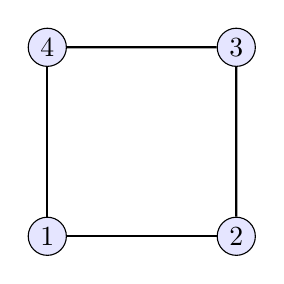
\begin{tikzpicture}[scale=1.2, node distance=2cm, every node/.style={circle, draw, fill=blue!10, inner sep=2pt}]
            \node (v1) at (0,0) {1};
            \node (v2) at (2,0) {2};
            \node (v3) at (2,2) {3};
            \node (v4) at (0,2) {4};
            \draw[thick] (v1) -- (v2);
            \draw[thick] (v2) -- (v3);
            \draw[thick] (v3) -- (v4);
            \draw[thick] (v4) -- (v1);
        \end{tikzpicture}
    \end{center}
    Matriks ketetanggaan $\*A$ untuk graf di atas adalah
    \[
        \*A =
        \begin{pmatrix}
            0 & 1 & 0 & 1 \\
            1 & 0 & 1 & 0 \\
            0 & 1 & 0 & 1 \\
            1 & 0 & 1 & 0
        \end{pmatrix}.
    \]
    Dengan kata lain, matriks derajatnya $\*D = \mathrm{diag}(2,2,2,2)$.
\end{contoh}

\begin{definisi}[\textbf{Graf Laplacian, \citep{chung1997}}]
    Graf Laplacian adalah $\*L=\*D-\*A$. Normalisasi simetris diberikan oleh
    \begin{equation}
        \*L_{\text{sym}} = \*I - \*D^{-1/2}\*A\*D^{-1/2}.
    \end{equation}
\end{definisi}

\noindent Graf Laplacian merepresentasikan struktur graf dan digunakan dalam berbagai algoritma GNN.

\begin{contoh}
    Misalkan graf $\mathcal{G}$ dengan $4$ simpul dan sisi $\mathcal{E} = \{(1,2), (2,3), (3,4), \allowbreak (4,1)\}$ (graf siklus). Matriks ketetanggaannya adalah
    \[
        \*A =
        \begin{pmatrix}
            0 & 1 & 0 & 1 \\
            1 & 0 & 1 & 0 \\
            0 & 1 & 0 & 1 \\
            1 & 0 & 1 & 0
        \end{pmatrix}
    \]
    dan matriks derajatnya adalah
    \[
        \*D = \mathrm{diag}(2,2,2,2).
    \]
    Graf Laplacian-nya dapat dihitung sebagai
    \[
        \*L = \*D - \*A =
        \begin{pmatrix}
            2 & -1 & 0 & -1 \\
            -1 & 2 & -1 & 0 \\
            0 & -1 & 2 & -1 \\
            -1 & 0 & -1 & 2
        \end{pmatrix}.
    \]
    Sehingga, dengan normalisasi simetris didapatkan
    \[
        \*L_{\text{sym}} = \*I - \frac{1}{2}\*A,
    \]
    karena $\*D^{-1/2} = \mathrm{diag}(1/\sqrt{2}, 1/\sqrt{2}, 1/\sqrt{2}, 1/\sqrt{2})$.
\end{contoh}


\begin{teorema}[\textbf{Teorema Spektral Laplacian, \citep{chung1997}}]
    Matriks Laplacian $\*L$ adalah simetris dan positif semidefinit, sehingga dapat didekomposisi dengan dekomposisi nilai eigen sebagai berikut.
    \begin{equation}
        \*L = \*U \bs\Lambda \*U^\top,
    \end{equation}
    dengan $\*U$ ortogonal dan $\bs\Lambda$ diagonal berisi nilai eigen
    $\lambda_1,\dots,\lambda_n \ge 0$. Selalu berlaku $\lambda_1=0$ dengan vektor
    eigen $\*1$.
\end{teorema}

\subsection{Kerangka Penyampaian Pesan pada Jaringan Saraf}

\begin{definisi}[\textbf{\emph{Message Passing Neural Networks} (MPNN), \citep{bronstein2021}}]
    Misalkan graf $\mathcal{G}=(\mathcal{V},\mathcal{E})$ dengan $\mathcal{V}$ adalah himpunan simpul dan $\mathcal{E}$ adalah himpunan sisi. Misalkan pula $\mathcal{N}_u$ adalah ketetanggaan simpul $u \in \mathcal{V}$. Lebih lanjut, misalkan $\bm x_u$ adalah fitur simpul $u$ dan $\bm e_{uv}$ adalah fitur sisi $(u,v) \in \mathcal{E}$. Suatu lapisan MPNN didefinisikan sebagai berikut.
    \begin{equation}
        \bm h_u = \varphi\left(\bm x_u, \bigoplus_{v \in \mathcal{N}_u}\psi(\bm x_u, \bm x_v, \bm e_{uv}),\right)
    \end{equation}
    dengan $\varphi$ dan $\psi$ adalah fungsi yang terdiferensiasi (seperti jaringan saraf) dan $\bigoplus$ adalah operator agregasi yang bersifat komutatif dan asosiatif (seperti penjumlahan atau rata-rata) atau \emph{permutation invariant}.
\end{definisi}

Kerangka MPNN ini sangat fleksibel dan dapat disesuaikan dengan berbagai jenis data graf. Fungsi $\psi$ dapat dirancang untuk menangkap interaksi spesifik antara simpul dan sisi, sedangkan fungsi $\varphi$ dapat berupa jaringan saraf yang kompleks untuk pembaruan fitur. Operator agregasi $\bigoplus$ memastikan bahwa model tetap invariant terhadap permutasi tetangga, yang penting dalam konteks graf. Beberapa arsitektur umum GNN, seperti \emph{Graph Convolutional Networks} (GCN) dan \emph{Graph Attention Networks} (GAT), dapat dianggap sebagai kasus khusus dari kerangka MPNN ini.

\subsection{Arsitektur Umum dalam GNN}

\begin{definisi}[\textbf{Graph Convolutional Networks (GCN), \citep{kipf2017}}]
    GCN mendefinisikan operasi propagasi lapisan ke-$l$ sebagai
    \begin{equation}
        \bm{H}^{(l+1)} = \sigma\!\left(\tilde{\*D}^{-1/2}\tilde{\*A}\tilde{\*D}^{-1/2}\bm{H}^{(l)} \*W^{(l)}\right),
    \end{equation}
    dengan:
    \begin{itemize}
        \item $\tilde{\*A} = \*A + \*I_n$ matriks ketetanggaan dengan \emph{self-loop},
        \item $\tilde{\*D} = \mathrm{diag}(\sum_j \tilde{A}_{ij})$ matriks derajat dari $\tilde{\*A}$,
        \item $\bm{H}^{(l)} \in \mathbb{R}^{n\times d_l}$ representasi simpul pada lapisan $l$,
        \item $\*W^{(l)} \in \mathbb{R}^{d_l \times d_{l+1}}$ bobot terlatih, dan
        \item $\sigma(\cdot)$ fungsi aktivasi non-linear.
    \end{itemize}
    GCN merupakan kasus khusus dari kerangka MPNN dengan:
    \begin{itemize}
        \item Fitur sisi diabaikan ($\bm e_{uv}$ tidak digunakan).
        \item Fungsi pesan $\psi(\bm x_u, \bm x_v, \bm e_{uv}) = \bm x_v$ (hanya mengambil fitur tetangga).
        \item Operator agregasi $\bigoplus$ berupa penjumlahan atau rata-rata tertimbang (melalui normalisasi Laplacian).
        \item Fungsi update $\varphi$ adalah komposisi linear dan aktivasi non-linear: $\varphi(\bm x_u, \mathrm{AGG}) = \sigma(\mathrm{AGG} \cdot \*W)$.
    \end{itemize}
    Secara eksplisit, propagasi GCN dapat ditulis sebagai
    \[
        \bm h_u^{(l+1)} = \sigma\left( \sum_{v \in \mathcal{N}_u \cup \{u\}} \frac{1}{\sqrt{d_u d_v}}\, \bm h_v^{(l)} \*W^{(l)} \right),
    \]
    dengan $d_u$ derajat simpul $u$ dan $\sigma$ fungsi aktivasi. Matriks normalisasi simetris $\tilde{\*D}^{-1/2}\tilde{\*A}\tilde{\*D}^{-1/2}$ merepresentasikan agregasi pesan dari tetangga dengan bobot yang sesuai, sehingga GCN adalah MPNN dengan agregasi rata-rata dan update linear.
\end{definisi}

\begin{definisi}[\textbf{Graph Attention Networks (GAT), \citep{velickovic2018}}]
    GAT mengganti normalisasi derajat dengan mekanisme perhatian.
    Koefisien perhatian untuk sisi $(i,j)$ adalah
    \begin{equation}
        \alpha_{ij} = \frac{\exp\!\left(\mathrm{LeakyReLU}\!\big(\bm{a}^\top [\*W\bm{h}_i \,\|\, \*W\bm{h}_j]\big)\right)}{\sum_{k \in \mathcal{N}(i)} \exp\!\left(\mathrm{LeakyReLU}\!\big(\*a^\top [\*W\bm{h}_i \,\|\, \*W\bm{h}_k]\big)\right)},
    \end{equation}
    dengan:
    \begin{itemize}
        \item $\bm{h}_i \in \mathbb{R}^{d}$ vektor fitur simpul $i$,
        \item $\*W$ bobot transformasi linear,
        \item $\bm{a} \in \mathbb{R}^{2d'}$ vektor bobot perhatian, dan
        \item $\|$ operator konkatenasi.
    \end{itemize}
    Pembaruan fitur simpul adalah
    \begin{equation}
        \*h_i' = \sigma\!\left(\sum_{j\in\mathcal{N}(i)} \alpha_{ij}\*W\bm{h}_j\right).
    \end{equation}
    GAT merupakan kasus khusus dari kerangka MPNN dengan spesifikasi berikut.
    \begin{itemize}
        \item Fitur sisi $\bm{e}_{uv}$ tidak digunakan (atau dapat diabaikan).
        \item Fungsi pesan $\psi(\bm{x}_u, \bm{x}_v, \bm{e}_{uv}) = \*W\bm{x}_v$ (transformasi linear fitur tetangga).
        \item Operator agregasi $\bigoplus$ berupa penjumlahan tertimbang, dengan bobot agregasi $\alpha_{uv}$ diperoleh dari mekanisme perhatian (\emph{attention}) yang bersifat permutation invariant.
        \item Fungsi update $\varphi$ adalah komposisi linear dan aktivasi non-linear: $\varphi(\bm{x}_u, \mathrm{AGG}) = \sigma(\mathrm{AGG})$.
    \end{itemize}
    Secara formal, pembaruan fitur simpul $u$ pada GAT dapat ditulis dalam notasi MPNN sebagai
    \begin{equation}
        \bm{h}_u' = \sigma\left(\sum_{v \in \mathcal{N}_u} \alpha_{uv} \psi(\bm{x}_u, \bm{x}_v, \bm{e}_{uv})\right)
        = \sigma\left(\sum_{v \in \mathcal{N}_u} \alpha_{uv} \*W\bm{x}_v\right),
    \end{equation}
    dengan $\alpha_{uv}$ adalah skor perhatian yang bergantung pada fitur $\bm{x}_u$ dan $\bm{x}_v$ melalui fungsi $\mathrm{LeakyReLU}(\*a^\top [\*W\bm{x}_u \,\|\, \*W\bm{x}_v])$ dan normalisasi softmax. Dengan demikian, GAT adalah MPNN dengan agregasi penjumlahan tertimbang dan fungsi pesan linear dengan bobot agregasi ditentukan secara adaptif oleh mekanisme perhatian.
\end{definisi}

\begin{definisi}[\textbf{GraphSAGE, \citep{hamilton2017}}]
    GraphSAGE atau \emph{Graph Sample and Aggregation} mendefinisikan pembaruan simpul $i$ sebagai
    \begin{equation}
        \bm h_i^{(l+1)} = \sigma\!\left(\bm W^{(l)} \cdot \mathrm{AGGREGATE}\left(\{\bm h_i^{(l)}\}\cup \{\bm h_j^{(l)}: j\in\mathcal{N}(i)\}\right)\right),
    \end{equation}
    dengan $\mathrm{AGGREGATE}$ fungsi agregasi non-linear yang bisa berupa
    \emph{mean}, \emph{max-pooling}, atau LSTM.
\end{definisi}

\subsection{Kekuatan Representasi GNN}

\begin{definisi}[\textbf{Isomorfisme Graf}]
    Dua graf $\mathcal{G}_1=(\mathcal{V}_1,\mathcal{E}_1)$ dan $\mathcal{G}_2=(\mathcal{V}_2,\mathcal{E}_2)$ disebut isomorfik jika terdapat bijeksi $\pi:\mathcal{V}_1 \to \mathcal{V}_2$ sehingga
    \begin{equation}
        (i,j)\in\mathcal{E}_1 \iff (\pi(i),\pi(j))\in\mathcal{E}_2.
    \end{equation}
    Sebuah fungsi $f$ dikatakan \emph{invarian terhadap isomorfisme graf} jika
    $f(\mathcal{G}_1)=f(\mathcal{G}_2)$ untuk setiap graf isomorfik
    $\mathcal{G}_1\cong \mathcal{G}_2$.
\end{definisi}

\begin{contoh}
    Misalkan $\mathcal{G}_1$ adalah graf dengan simpul $\{1,2,3\}$ dan sisi $\{(1,2), \allowbreak (2,3),(3,1)\}$ (graf segitiga). Ambil $\mathcal{G}_2$ dengan simpul $\{a,b,c\}$ dan sisi $\{(a,b),\allowbreak(b,c),(c,a)\}$. Bijeksi $\pi$ dapat dipilih misal $\pi(1)=a$, $\pi(2)=b$, $\pi(3)=c$. Maka $\mathcal{G}_1$ dan $\mathcal{G}_2$ isomorfik.

    Sebagai contoh fungsi invarian, jumlah simpul $|\mathcal{V}|$ dan jumlah sisi $|\mathcal{E}|$ adalah invarian terhadap isomorfisme graf. Demikian juga, spektrum Laplacian graf $\*L$ adalah invarian terhadap isomorfisme.

    \begin{figure}[H]
        \centering
        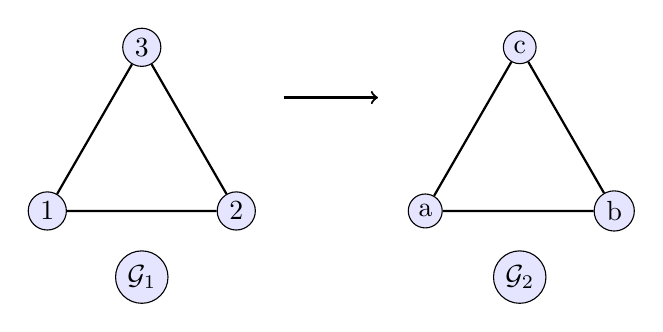
\begin{tikzpicture}[scale=1.2, node distance=2cm, every node/.style={circle, draw, fill=blue!10, inner sep=2pt}]
            % Graph G1
            \node (v1) at (0,0) {1};
            \node (v2) at (2,0) {2};
            \node (v3) at (1,1.732) {3};
            \draw[thick] (v1) -- (v2) -- (v3) -- (v1);
            \node at (1,-0.7) {$\mathcal{G}_1$};

            % Arrow for isomorphism
            \draw[->, thick] (2.5,1.2) -- (3.5,1.2);
            \node (a) at (4,0) {a};
            \node (b) at (6,0) {b};
            \node (c) at (5,1.732) {c};
            \draw[thick] (a) -- (b) -- (c) -- (a);
            \node at (5,-0.7) {$\mathcal{G}_2$};
        \end{tikzpicture}
        \caption{Ilustrasi dua graf isomorfik, yaitu $\mathcal{G}_1$ dan $\mathcal{G}_2$ memiliki struktur yang sama walaupun label simpul berbeda. (Sumber: Dokumen penulis)}
    \end{figure}
\end{contoh}

\begin{definisi}[\textbf{Tes Weisfeiler--Lehman (WL) Satu Dimensi}]
    Algoritma WL satu dimensi, juga dikenal sebagai \emph{color refinement}, merupakan prosedur iteratif untuk membedakan graf berdasarkan struktur lokal simpul. Pada setiap iterasi, label simpul $h_i^{(t)}$ diperbarui dengan cara:
    \begin{equation}
        h_i^{(t+1)} = \mathrm{HASH}\!\left(h_i^{(t)}, \{h_j^{(t)} : j \in \mathcal{N}(i)\}\right),
    \end{equation}
    dimulai dari label awal $h_i^{(0)}$. Dua graf dikatakan dapat dibedakan oleh tes WL jika multiset label akhirnya berbeda. Dalam konteks pembelajaran mesin, tes WL memberikan kerangka formal untuk mengukur kemampuan model, seperti GNN, dalam membedakan struktur graf yang berbeda melalui proses agregasi informasi dari tetangga.
\end{definisi}

Fungsi $\mathrm{HASH}$ pada algoritma WL berperan sebagai pemetaan yang menggabungkan label simpul saat ini dengan label-label tetangganya menjadi label baru yang unik. Intuisi utamanya adalah memastikan bahwa jika dua simpul memiliki lingkungan yang berbeda, hasil $\mathrm{HASH}$ juga berbeda. Dalam implementasi praktis, $\mathrm{HASH}$ dapat berupa fungsi injektif seperti pengkodean \emph{string}, \emph{concatenation}, atau fungsi neural yang mampu membedakan multiset masukan secara efektif.

\begin{teorema}[\textbf{Keterbatasan GNN Berbasis Agregasi, \citep{xu2019}}]
    GNN berbasis agregasi dengan pembaruan umum
    \begin{equation}
        h_i^{(l+1)} = \varphi\!\left( W^{(l)} \cdot \mathrm{AGGREGATE}\big(\{h_i^{(l)}\}\cup\{h_j^{(l)}: j\in \mathcal{N}(i)\}\big)\right)
    \end{equation}
    tidak lebih kuat daripada tes WL satu dimensi dalam membedakan graf yang tidak isomorfik. Artinya, kemampuan GNN untuk membedakan struktur graf dibatasi oleh kekuatan agregasi lokal yang serupa dengan tes WL.
\end{teorema}

\begin{teorema}[\textbf{Hubungan dengan Tes WL, \citep{xu2019}}]
    Jika fungsi agregasi $\mathrm{AGGREGATE}$ bersifat injektif terhadap multiset, maka GNN memiliki kekuatan representasi setara dengan tes WL satu dimensi. Dengan kata lain, GNN dapat membedakan graf sejauh tes WL mampu membedakannya, asalkan agregasi dan pembaruan fitur dilakukan secara unik untuk setiap lingkungan simpul.
\end{teorema}